
%================================================================
%  RAPPORT DE FIN D'ÉTUDES — Fichier principal
%================================================================
\documentclass[12pt,a4paper,twoside]{report}

\setcounter{secnumdepth}{4}

%----------------------------------------------------------------
%  1. Encodage et langue
%----------------------------------------------------------------
\usepackage[T1]{fontenc}
\usepackage[utf8]{inputenc}
\usepackage[french]{babel}

%----------------------------------------------------------------
%  2. Mise en page
%----------------------------------------------------------------
\usepackage[
top=2.5cm,
bottom=2.5cm,
inner=3cm,
outer=2.5cm
]{geometry}

\usepackage{graphicx}
\usepackage[export]{adjustbox}
\usepackage[hidelinks]{hyperref}
\usepackage[final]{pdfpages}
\usepackage{float}
\usepackage{pslatex}
\usepackage[table]{xcolor}
\usepackage{array}
\usepackage{setspace}
\usepackage{enumerate}
\usepackage{enumitem}
\usepackage{longtable}
\usepackage{multirow}
\usepackage[font=small,labelfont=bf]{caption}
\usepackage{minitoc}
\usepackage[Glenn]{fncychap}
\usepackage{tabularx}
\usepackage{microtype}
\usepackage{titlesec}

%----------------------------------------------------------------
%  3. En-têtes et pieds de page
%----------------------------------------------------------------
\usepackage{fancyhdr}

\setlength{\headheight}{15.5pt}
\addtolength{\topmargin}{-3.5pt}

\pagestyle{fancy}
\fancyhf{}

% Header
\fancyhead[LE,RO]{\nouppercase{\leftmark}}

% Footer
\fancyfoot[LE,RO]{\thepage}
\fancyfoot[L]{HR FaceTime --- Rapport PFE}

\renewcommand{\headrulewidth}{0.4pt}
\renewcommand{\footrulewidth}{0.4pt}

% Style des pages "plain"
\fancypagestyle{plain}{
    \fancyhf{}
    \fancyhead[LE,RO]{\nouppercase{\leftmark}}
    \fancyfoot[LE,RO]{\thepage}
    \fancyfoot[L]{HR FaceTime --- Rapport PFE}
    \renewcommand{\headrulewidth}{0.4pt}
    \renewcommand{\footrulewidth}{0.4pt}
}

%----------------------------------------------------------------
%  4. Espacement et typographie
%----------------------------------------------------------------

\onehalfspacing

% Paragraphes
\setlength{\parindent}{1.25cm}
\setlength{\parskip}{0.3em}

% Figures et tableaux
\setlength{\floatsep}{12pt}
\setlength{\textfloatsep}{15pt}
\setlength{\intextsep}{12pt}

% Longtable
\setlength{\LTpre}{8pt}
\setlength{\LTpost}{8pt}

% Tableaux plus lisibles
\renewcommand{\arraystretch}{1.25}

% Listes
\setlist{
    itemsep=4pt,
    topsep=6pt,
    parsep=0pt
}

% Captions professionnelles
\captionsetup{
    font=small,
    labelfont=bf,
    justification=centering,
    skip=8pt
}

% Espacement des titres
\titlespacing*{\chapter}
{0pt}{-15pt}{30pt}

\titlespacing*{\section}
{0pt}{18pt}{8pt}

\titlespacing*{\subsection}
{0pt}{14pt}{6pt}

% Évite les grandes zones blanches
\raggedbottom

%----------------------------------------------------------------
%  5. DOCUMENT
%----------------------------------------------------------------
\begin{document}

\dominitoc

%==============================================================
% FRONT MATTER
%==============================================================

\cleardoublepage
\pagenumbering{roman}
\pagestyle{fancy}

\chapter*{Dédicaces}
\addcontentsline{toc}{chapter}{Dédicaces}

\begin{center}
\begin{minipage}{0.9\textwidth}
\itshape

Ce travail est pour ----------------, le père de mes rêves.\\
Grâce à vous, je suis comblé de votre soutien et de votre amour.\\
Tous les sacrifices que vous avez consentis pour mon éducation sont le prix que je coûte à ce travail.

\vspace{0.4cm}

À ma mère ---------------,\\
Je peine à trouver les mots qui traduisent ma grande estime pour tant d'amour, d'encouragement.\\
La figure de l'admiration et de la motivation que vous représentez à mes yeux.

\vspace{0.4cm}

--------------------, mes frères bien-aimés,\\
Qui êtes toujours là pour moi et qui m'ont soutenu dans mes moments les plus probants.\\
Je vous souhaite la réussite et le bonheur.

\vspace{0.4cm}

-----------------, mon grand-père,\\
Qui m'a aidé et m'a toujours encouragé à donner le meilleur de moi-même.

\vspace{0.4cm}

À l'âme de ma grand-mère -----------------,\\
Qu'Allah lui accorde Sa miséricorde et l'accueille dans Son paradis éternel.

\vspace{0.4cm}

À mes amis et à toute ma famille,\\
Pour leur soutien et leur amitié sincère.

\end{minipage}
\end{center}

\cleardoublepage
\begin{titlepage}
\thispagestyle{empty}
\vspace*{0.5cm}
\begin{center}
{\Huge \textbf{Remerciements}}
\end{center}
\vspace{0.5cm}

Nous remercions avant tout \textbf{Allah}, le Tout-Puissant et le
Miséricordieux, de nous avoir accordé la patience et la volonté d'accomplir ce travail. C'est grâce à Sa grâce et Sa
miséricorde que nous sommes parvenues à l'aboutissement de ce projet.
Que toute louange Lui revienne.
Nous tenons ensuite à exprimer notre profonde gratitude à toutes les
personnes qui ont contribué au bon déroulement de notre projet de fin
d'études et qui nous ont accompagnées tout au long de cette expérience
enrichissante.

\vspace{0.3cm}

Nous adressons nos sincères remerciements à notre encadrant académique,
\textbf{Dr. Amara Hiba}, pour son encadrement rigoureux, sa disponibilité,
ses conseils précieux ainsi que l'attention particulière qu'il a portée à
notre travail. Son accompagnement et ses orientations pertinentes nous ont
été d'une aide précieuse durant la réalisation de ce projet.

\vspace{0.3cm}

Nous exprimons également notre reconnaissance à notre encadrant professionnel,
\textbf{Mr. BelHadj Mohamed}, pour son accueil chaleureux au sein de
l'équipe \textbf{UNIBRO Distribution Plus}, sa confiance, son professionnalisme ainsi
que pour les connaissances et l'expérience qu'il nous a transmis tout au long
de cette période de stage. Sa disponibilité, sa pédagogie et sa passion pour
son domaine ont été une source d'inspiration constante. Ses conseils avisés,
son suivi rigoureux et sa capacité à nous guider avec bienveillance nous ont
permis de développer nos compétences techniques et professionnelles dans un
environnement à la fois motivant, stimulant et enrichissant.

\vspace{0.3cm}

Enfin, nous exprimons notre gratitude envers nos familles et nos amis pour
leur soutien moral, leurs encouragements permanents et leur confiance tout
au long de notre parcours universitaire.

\vspace{0.4cm}
\begin{flushright}
\textbf{Araar Mohamed}\\
\textbf{Mejri Louay}
\end{flushright}
\end{titlepage}

\cleardoublepage
\tableofcontents

\cleardoublepage
\listoffigures

\cleardoublepage
\listoftables

\mtcaddchapter

%==============================================================
% MAIN MATTER
%==============================================================

\cleardoublepage
\pagenumbering{arabic}
\pagestyle{fancy}

\chapter*{Introduction Générale}
%ajouter le titre introduction générale dans la table des matières
\addcontentsline{toc}{chapter}{Introduction Générale}
%définir l'entête de ce chapitre 
\markboth{Introduction Générale}{}
\setlength{\intextsep}{6pt}
\setlength{\textfloatsep}{8pt}
\setlength{\floatsep}{6pt}
\setlength{\abovecaptionskip}{3pt}
\setlength{\belowcaptionskip}{1pt}
\setlength{\LTpre}{3pt}
\setlength{\LTpost}{3pt}

À l’ère de la transformation numérique, la gestion des ressources humaines s’impose comme l’un des domaines les plus stratégiques au sein des organisations modernes. Couvrant des processus essentiels tels que le suivi des présences, la gestion des congés, l’administration des salaires et le traitement des documents administratifs, elle influence directement la performance opérationnelle ainsi que le bien-être des collaborateurs. Toutefois, lorsque ces processus reposent encore sur des méthodes manuelles ou des outils traditionnels, ils engendrent souvent des erreurs, des pertes de temps et un manque de transparence pouvant nuire au bon fonctionnement de l’entreprise. Dans ce contexte, l’intégration des technologies intelligentes, notamment la reconnaissance faciale, représente une solution innovante permettant d’automatiser les tâches, d’améliorer la fiabilité des traitements et d’optimiser la gestion du personnel. La digitalisation des processus RH devient ainsi une nécessité incontournable pour les entreprises souhaitant améliorer leur efficacité et renforcer leur compétitivité.

Dans ce cadre, nous avons eu l’opportunité de réaliser notre Projet de Fin d’Études au sein de la société UNIBRO Distribution, entreprise spécialisée dans la distribution de produits alimentaires et de grande consommation. Notre mission a consisté à concevoir et développer un Logiciel RH Intelligent de Pointage Automatique, visant à moderniser et centraliser la gestion des ressources humaines au sein de l’entreprise. Le fonctionnement de cette application repose sur une plateforme web sécurisée accessible selon trois profils utilisateurs : Administrateur, Responsable RH et Employé. Après authentification, chaque utilisateur accède à un espace dédié contenant les fonctionnalités correspondant à son rôle. Le système intègre un module de reconnaissance faciale permettant d’identifier automatiquement les employés via des caméras connectées à la plateforme. Lorsqu’un employé se présente devant la caméra, son visage est analysé puis comparé aux données biométriques enregistrées afin de valider automatiquement son pointage d’entrée ou de sortie en temps réel. En complément du pointage intelligent, l’application offre un ensemble de services RH tels que la gestion des congés, des absences, des primes, des déductions, des salaires et des documents administratifs. Les responsables RH disposent de tableaux de bord interactifs leur permettant de superviser les données du personnel, de générer des rapports et de suivre les indicateurs de présence, tandis que les employés peuvent consulter leurs informations personnelles et effectuer leurs demandes de manière autonome. Afin d’assurer performance, sécurité et évolutivité, la solution a été développée à l’aide des technologies Next.js, Flask et MySQL, tout en suivant la méthodologie agile Scrum pour garantir une organisation efficace du projet.

Ce rapport est organisé en quatre chapitres principaux. Le premier chapitre donne un aperçu général du projet, de l’organisation d’accueil, de l’étude de l’existant et de la méthodologie du projet. Le deuxième chapitre est consacré à l’analyse des besoins du système, à sa description fonctionnelle et non fonctionnelle, à la définition de son architecture et de sa stratégie de réalisation suivant le processus Scrum. Le troisième chapitre aborde la première release du projet, qui comprend la gestion des accès, la gestion des comptes et la réalisation de la fonctionnalité de pointage par reconnaissance faciale. Enfin, le quatrième chapitre concerne la deuxième release du projet, consacrée aux fonctionnalités avancées de gestion de personnel, aux tableaux de bord et aux reportings du projet.
\clearpage
\mtcaddchapter
\mtcaddchapter

\chapter{Présentation du cadre du projet}
\setlength{\intextsep}{6pt}
\setlength{\textfloatsep}{8pt}
\setlength{\floatsep}{6pt}
\setlength{\abovecaptionskip}{3pt}
\setlength{\belowcaptionskip}{1pt}
\setlength{\LTpre}{3pt}
\setlength{\LTpost}{3pt}

\newpage

\section{Introduction}
Ce premier chapitre comportera plusieurs parties dont on peut citer l’organisme d’accueil, la 
problématique du projet, la solution proposée ainsi que notre méthodologie adoptée pour le développement de ce projet.

\section{Présentation de l'organisme d'accueil}
Notre projet se déroule au sein de l’entreprise UNIBRO Distribution Plus, une société spécialisée dans la distribution de produits alimentaires et de grande consommation. Elle se distingue par son organisation logistique, son professionnalisme et sa capacité à répondre efficacement aux besoins du marché. UNIBRO Distribution Plus s’engage à assurer un service fiable, basé sur la qualité, la rapidité et la satisfaction de ses partenaires commerciaux.\cite{ref1}
\begin{figure}[H]
  \centering
    
\includegraphics[scale=0.3]{projet/images/logo_unibro-removebg-preview}
  \caption{Logo de la société UNIBRO Distribution Plus}
\end{figure}
\subsection{Domaines d’activités}
UNIBRO Distribution Plus se spécialise dans les domaines suivants :
\begin{itemize}[label=$\rightarrow$]
\item 
 Distribution de produits : Approvisionnement et distribution de produits alimentaires et de grande consommation.
\item 
 Logistique : Gestion du transport, du stockage et de la livraison des marchandises.
\item 
 Gestion commerciale : Relations avec les fournisseurs et les clients, suivi des commandes et des ventes.
\item Service client : Satisfaction des partenaires commerciaux et respect des délais de livraison.
\end{itemize}

\section{Contexte du projet}
Dans cette partie, nous décrivons l'étude de l'existant, les limites ainsi que la solution proposée.
\subsection{Etude de l'existant}
Cette section présente une analyse du système existant de gestion du pointage et des procédures RH, en mettant en évidence ses principales caractéristiques ainsi que ses limites. 
\subsubsection{Description de l'existant}
Le système actuel de gestion du pointage et des procédures RH repose sur des méthodes traditionnelles :
\begin{itemize}
\item Les registres manuels (feuilles de présence) : Les employés signent un document papier à l’arrivée et au départ.

\item  Les systèmes à badges (RFID/Magnétiques) : L’identification repose sur la possession d’une carte que l’employé passe devant un lecteur.

\item L’authentification par codes (PIN) : L’employé saisit un code personnel sur un clavier numérique.
\item Justification d’absence physique : Les justificatifs sont remis manuellement sans dépôt ni archivage numérique.
\item Gestion traditionnelle des primes : L’attribution et le suivi des primes sont effectués manuellement sans consultation numérique pour les employés.
\item Absence de consultation du salaire mensuel : Les employés ne peuvent pas vérifier le statut de leur salaire du mois en cours.

\end{itemize}

\subsubsection{Critique de l'existant et problématique}
Nous citons ci-dessous quelques problèmes liés au système existant :
%===========utiliser une liste à puces simple 
\begin{itemize}
 \item  Erreur humaine : saisie manuelle sujette à des oublis ou des erreurs.

\item Fraude : possibilité de pointage pour un autre employé.

\item Pas de suivi en temps réel : impossibilité de visualiser immédiatement la présence ou l’absence.

\item Gestion lourde : centralisation et analyse des données complexes et fastidieuses..
\item Procédures administratives lentes dues à l’utilisation de documents papier. 
\item Manque de transparence pour les employés concernant les congés, absences, primes et salaires. 
\item Risque de perte ou de détérioration des documents physiques.
\end{itemize}

\subsection{Solution proposée}
Afin de résoudre le problème mentionné plus haut lors de ce projet de fin d'études,
nous allons nous concentrer sur la réalisation d'un logiciel intelligent de gestion des ressources humaines de pointage automatique avec reconnaissance faciale.
Cela aidera à créer un emplacement centralisé pour organiser toute information relative à la gestion des données de présence de nos employés.
Les employés du département de gestion des ressources humaines auront l'opportunité de recevoir des rapports détaillés en peu de temps, parmi lesquels ils seront capables de suivre l'indicateur de présence, de retard ou d'absence des employés.
Le processus comprend les éléments suivants :
\begin{enumerate}
    \item  Collecte de données : prise en charge de la photo du visage des employés avec caméra.
\item   Intégration et traitement des données : enregistrement automatique de la présence des employés avec indication de leur heures d'entrée et de sortie.
\item  Traitement et analyse des données : visualisation et suivi des statistiques avec l'aide d'une interface intuitive de tableau de bord.
\end{enumerate}
À l'aide de ce système d'information, l'entreprise aura une occasion d'optimiser la gestion de son personnel et de supprimer les erreurs dans le processus de pointage des employés.


%=========================================
% Méthodologie de travail
%=========================================

\section{Méthodologie de travail}

Une méthodologie de gestion de projet est un cadre qui guide les équipes dans la planification, l’exécution et la finalisation d’un projet. Elle définit les processus et les outils à utiliser, et son choix dépend de la nature et des besoins spécifiques du projet.

Parmi les méthodologies les plus connues, on distingue :

\begin{itemize}
    \item \textbf{Les méthodes agiles :} La méthode Agile est une approche itérative de la gestion de projet qui privilégie la flexibilité, la collaboration et la livraison régulière de valeur. Née en 2001 avec le Manifeste Agile, elle s’oppose aux projets figés en cherchant à apprendre vite, ajuster en continu et intégrer le client dans la boucle.

    \item \textbf{Les méthodes traditionnelles :} La méthode traditionnelle de gestion de projet est une approche de développement basée sur une planification séquentielle des différentes phases du projet. Chaque étape, telle que l’analyse des besoins, la conception, le développement, les tests et le déploiement, doit être complétée avant de passer à la suivante. Cette méthode repose sur une organisation rigide et une planification détaillée dès le début du projet.
\end{itemize}

Le choix entre une méthode agile et une méthode traditionnelle ne se fait pas de façon arbitraire, mais doit être fondé sur les besoins spécifiques du projet.

\subsection{Étude comparative}

Nous présentons dans le tableau suivant une étude comparative entre les méthodes traditionnelles et les méthodes agiles.

\renewcommand{\arraystretch}{1.3}

\begin{longtable}{|p{2.5cm}|p{6cm}|p{6cm}|}

\hline
\textbf{Critère} & \textbf{Méthode traditionnelle} & \textbf{Méthode agile} \\
\hline
\endhead

Planification &
Basée sur une planification détaillée réalisée au début du projet. Toutes les étapes sont définies à l’avance. &
Planification flexible qui évolue au fur et à mesure du projet en fonction des besoins et des retours des utilisateurs. \\
\hline

Organisation du projet &
Approche séquentielle où chaque phase doit être terminée avant de passer à la suivante. &
Approche itérative et incrémentale basée sur des cycles de développement courts appelés itérations ou sprints. \\
\hline

Gestion des changements &
Les changements sont difficiles à intégrer une fois le projet lancé. &
Les changements peuvent être facilement intégrés à chaque itération du projet. \\
\hline

Implication du client &
Le client intervient principalement au début pour définir les besoins et à la fin pour valider le produit. &
Le client est impliqué tout au long du projet et participe régulièrement aux validations. \\
\hline

Livraison du produit &
Le produit final est livré à la fin du projet après la réalisation de toutes les phases. &
Le produit est livré progressivement sous forme de versions fonctionnelles après chaque itération. \\
\hline

Flexibilité &
Faible flexibilité face aux changements ou aux nouvelles exigences. &
Grande flexibilité permettant d’adapter le projet aux évolutions des besoins. \\
\hline

Gestion des risques &
Les risques sont souvent détectés tardivement dans le projet. &
Les risques sont identifiés et traités plus rapidement grâce aux cycles courts de développement. \\
\hline

Communication &
Communication souvent formelle et basée sur la documentation. &
Communication continue entre les membres de l’équipe et les parties prenantes. \\
\hline
\caption{Comparaison entre les méthodes traditionnelles et les méthodes agiles}
\end{longtable}
Après une étude préliminaire, la méthodologie la plus adaptée à notre projet est la méthodologie Agile. Toutefois, il reste nécessaire de déterminer quel framework Agile est le plus approprié pour notre projet. À cet effet, le tableau suivant présente une comparaison entre les principaux frameworks Agile les plus utilisés.

\renewcommand{\arraystretch}{1.3}

\begin{longtable}{|p{2cm}|p{4cm}|p{4cm}|p{4cm}|}

\hline
\textbf{Critère} & \textbf{Scrum} & \textbf{Kanban} & \textbf{Extreme Programming (XP)} \\
\hline
\endhead

Objectif &
Gestion du développement par itérations courtes (sprints). &
Optimisation et visualisation du flux de travail. &
Amélioration continue de la qualité du code. \\
\hline

Organisation du travail &
Travail structuré en sprints (1 à 4 semaines). &
Flux de travail continu sans sprints. &
Itérations très courtes avec livraisons fréquentes. \\
\hline

Gestion des tâches &
Product Backlog et Sprint Backlog. &
Tableau Kanban (À faire, En cours, Terminé). &
Développement progressif avec tests continus. \\
\hline

Rôles &
Product Owner, Scrum Master, équipe de développement. &
Pas de rôles imposés. &
Collaboration étroite entre développeurs et client. \\
\hline

Réunions &
Sprint Planning, Daily Scrum, Sprint Review et Sprint Retrospective. &
Peu de réunions formelles. &
Réunions fréquentes pour le retour d'expérience (feedback). \\
\hline

Gestion des changements &
Changements intégrés entre les sprints. &
Changements possibles à tout moment. &
Adaptation rapide grâce aux cycles courts. \\
\hline

Visualisation &
Tableau Scrum ou outils de backlog. &
Tableau Kanban visuel. &
Suivi intégré au processus de développement. \\
\hline

Limitation du travail &
Possible selon l’organisation de l’équipe. &
Limitation stricte du travail en cours (WIP). &
Limitation naturelle grâce aux itérations courtes. \\
\hline

Qualité du code &
Pas de pratiques techniques imposées. &
Pas de règles techniques spécifiques. &
Forte priorité accordée à la qualité du code. \\
\hline

Pratiques techniques &
Dépend de l’équipe. &
Non définies. &
TDD, Pair Programming, intégration continue et tests automatisés. \\
\hline

Projets adaptés &
Projets complexes nécessitant une organisation structurée. &
Activités continues telles que la maintenance et le support. &
Projets logiciels exigeant une haute qualité du code. \\
\hline
\caption{Comparaison entre les frameworks Agile : Scrum, Kanban et Extreme Programming (XP)}
\end{longtable}

\subsubsection{Choix de l’approche}

Après comparaison des différentes méthodologies, notre choix s’est porté sur le framework SCRUM. Ce dernier favorise une organisation structurée grâce à des réunions régulières, notamment le \textit{Daily Scrum}, permettant de suivre l’avancement, d’identifier rapidement les obstacles et de maintenir la productivité de l’équipe. Il facilite également une meilleure planification et un suivi continu des tâches, contribuant ainsi au respect des délais du projet.

\subsubsection{L’approche SCRUM pour le développement du projet}

La méthode SCRUM organise le travail en cycles courts appelés \textit{Sprints}, d’une durée de deux à quatre semaines. À l’issue de chaque Sprint, une version partielle mais fonctionnelle du produit est livrée, permettant d’évaluer l’avancement et d’apporter les améliorations nécessaires. La figure ci-dessous \cite{scrum_guide} illustre le cycle de vie de la méthode SCRUM.

\begin{figure}[h!]
    \centering
    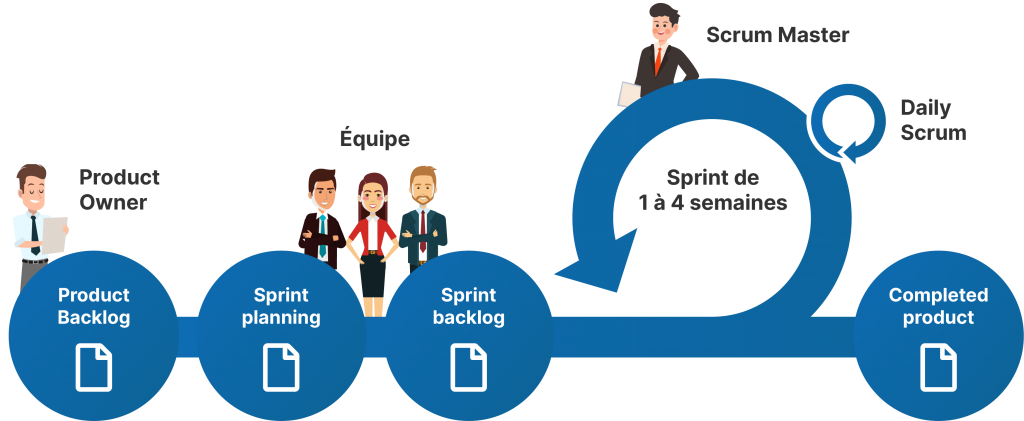
\includegraphics[width=0.8\textwidth]{projet/images/scrum.png}
    \caption{Cycle de vie SCRUM \cite{scrum_guide}}
    \label{fig:scrum_cycle}
\end{figure}

\textbf{Rôles clés :}

\begin{itemize}
    \item \textbf{Product Owner :} Il représente la voix du client au sein de l’équipe. Son rôle consiste à recueillir et analyser les besoins des utilisateurs, puis à les traduire sous forme de User Stories. Il est également responsable de la priorisation des tâches dans le Product Backlog et veille à ce que les fonctionnalités développées répondent aux attentes des utilisateurs.

    \item \textbf{Équipe de développement :} Elle est composée de plusieurs membres chargés de concevoir et réaliser les fonctionnalités définies par le Product Owner. L’équipe est auto-organisée et collaborative, chaque membre contribuant activement à l’atteinte des objectifs du Sprint.

    \item \textbf{Scrum Master :} Il agit comme facilitateur du processus Scrum. Son rôle est de s’assurer de la bonne application des principes Agile, d’aider l’équipe à surmonter les obstacles rencontrés et de garantir le bon déroulement des Sprints afin de maintenir une progression efficace du projet.
\end{itemize}

La méthode Scrum s’appuie également sur des éléments clés appelés artefacts Scrum, qui permettent d’organiser le travail, de suivre l’avancement du projet et d’assurer la transparence au sein de l’équipe.

 
\section{Conclusion}

Ce chapitre constitue une étape primordiale pour fixer les repères de notre projet durant lequel nous avons présenté l’organisme d’accueil et dégagé des attentes du projet après avoir étudié et critiqué l’existant. À la fin, nous avons présenté la méthodologie de travail à utiliser.
 



\chapter{Analyse et spécification des besoins}
\setlength{\intextsep}{6pt}
\setlength{\textfloatsep}{8pt}
\setlength{\floatsep}{6pt}
\setlength{\abovecaptionskip}{3pt}
\setlength{\belowcaptionskip}{1pt}
\setlength{\LTpre}{3pt}
\setlength{\LTpost}{3pt}

\newpage

%============================================================
\section{Introduction}
%============================================================

Le présent chapitre est dédié à la description des exigences fonctionnelles et non
fonctionnelles du logiciel de gestion des ressources humaines et de pointage automatique
par reconnaissance faciale. Ce chapitre contient l'information relative à l'environnement
logiciel, matériel et technologique requis pour le développement et l'utilisation du
logiciel proposé. Aussi, le chapitre contient la description de la méthodologie du travail
utilisée et basée sur la méthode Agile Scrum.

%============================================================
\section{Analyse des besoins}
%============================================================

Dans cette partie, nous détaillons les besoins du système, en identifiant les
fonctionnalités attendues ainsi que les contraintes techniques, sécuritaires et
ergonomiques associées.

\subsection{Besoins fonctionnels}

Les besoins fonctionnels du système de gestion RH et de pointage basé sur la reconnaissance
faciale correspondent aux différentes actions que chaque utilisateur doit pouvoir réaliser
pour que le système remplisse ses objectifs. Pour les formaliser, nous avons identifié les
acteurs et les cas d'utilisation du système conformément aux standards UML.

\subsubsection{Identification des acteurs}

L'analyse du système a permis de définir trois acteurs principaux :

\begin{itemize}
  \item \textbf{Employé :} Personne travaillant dans l'entreprise.
  \item \textbf{Responsable RH :} Membre du personnel ayant des droits spécifiques pour
        gérer les employés, les dossiers RH et générer des rapports.
  \item \textbf{Administrateur du logiciel :} Personne chargée de superviser la plateforme,
        de gérer les utilisateurs et leurs accès.
\end{itemize}

\subsubsection{Identification des cas d'utilisation}

Pour chaque acteur, les objectifs et fonctionnalités du système sont les suivants :

\paragraph{Fonctionnalités pour l'employé}

\begin{itemize}
  \item Enregistrer son visage : permettre à l'employé d'ajouter ses données faciales dans le système.
  \item Modifier ses informations personnelles : mettre à jour ses informations telles que l'adresse, le numéro de téléphone ou l'état civil.
  \item Consulter ses absences : visualiser son historique d'absences et de présences.
  \item Pointage faciale : effectuer l'enregistrement de présence à l'aide de la reconnaissance faciale.
  \item Consulter son salaire : accéder aux informations relatives à sa rémunération.
  \item Soumettre un  congé : soumettre une demande de congé au service concerné.
  \item Consulter historique : afficher les opérations et actions précédemment effectuées.
  \item Déposer un document : envoyer des fichiers ou justificatifs au système.
  
\end{itemize}

\paragraph{Fonctionnalités pour le responsable RH}

\begin{itemize}
  \item S'inscrire : permettre au responsable RH de créer un compte et d'accéder aux fonctionnalités dédiées.
  \item Visualiser le Dashboard RH : consulter les indicateurs clés, statistiques des employés et synthèses RH.
  \item Connexion de la plateforme aux caméras : configurer et gérer les flux vidéo pour la reconnaissance faciale.
  \item Gérer les comptes employés : ajouter, modifier, désactiver ou supprimer les profils des employés.
  \item Gérer les congés (validation / refus) : traiter les demandes de congé, les approuver ou les refuser et suivre leur historique.
  \item Gérer les salaires : consulter et mettre à jour les informations de paie et générer des fiches de salaire.
  \item Gérer les documents : superviser le dépôt, le classement et l'accès aux justificatifs et pièces administratives.
  \item Gérer historique et rapports : générer, consulter et exporter les rapports d'activité, d'absence et autres historiques.
\end{itemize}

\paragraph{Fonctionnalités pour l'administrateur}

\begin{itemize}
  \item Gérer les comptes des utilisateurs (responsable RH) du système : créer, modifier, désactiver ou supprimer les comptes des responsables RH afin de contrôler leur accès à la plateforme.
  \item Visualiser le Dashboard Administrateur : consulter les indicateurs globaux, les statistiques d'utilisation et les informations de supervision du système.
  
\end{itemize}

\subsubsection{Diagramme de cas d'utilisation global}

Toutes les fonctionnalités mentionnées précédemment pour les différents acteurs (Employé,
Responsable RH et Administrateur du logiciel) ont été regroupées dans un diagramme de cas
d'utilisation. Ce diagramme structuré permet de visualiser les interactions entre les
acteurs et le système. La figure~\ref{fig:usecase} présente ce diagramme de cas d'utilisation.

\begin{figure}[H]
  \centering
  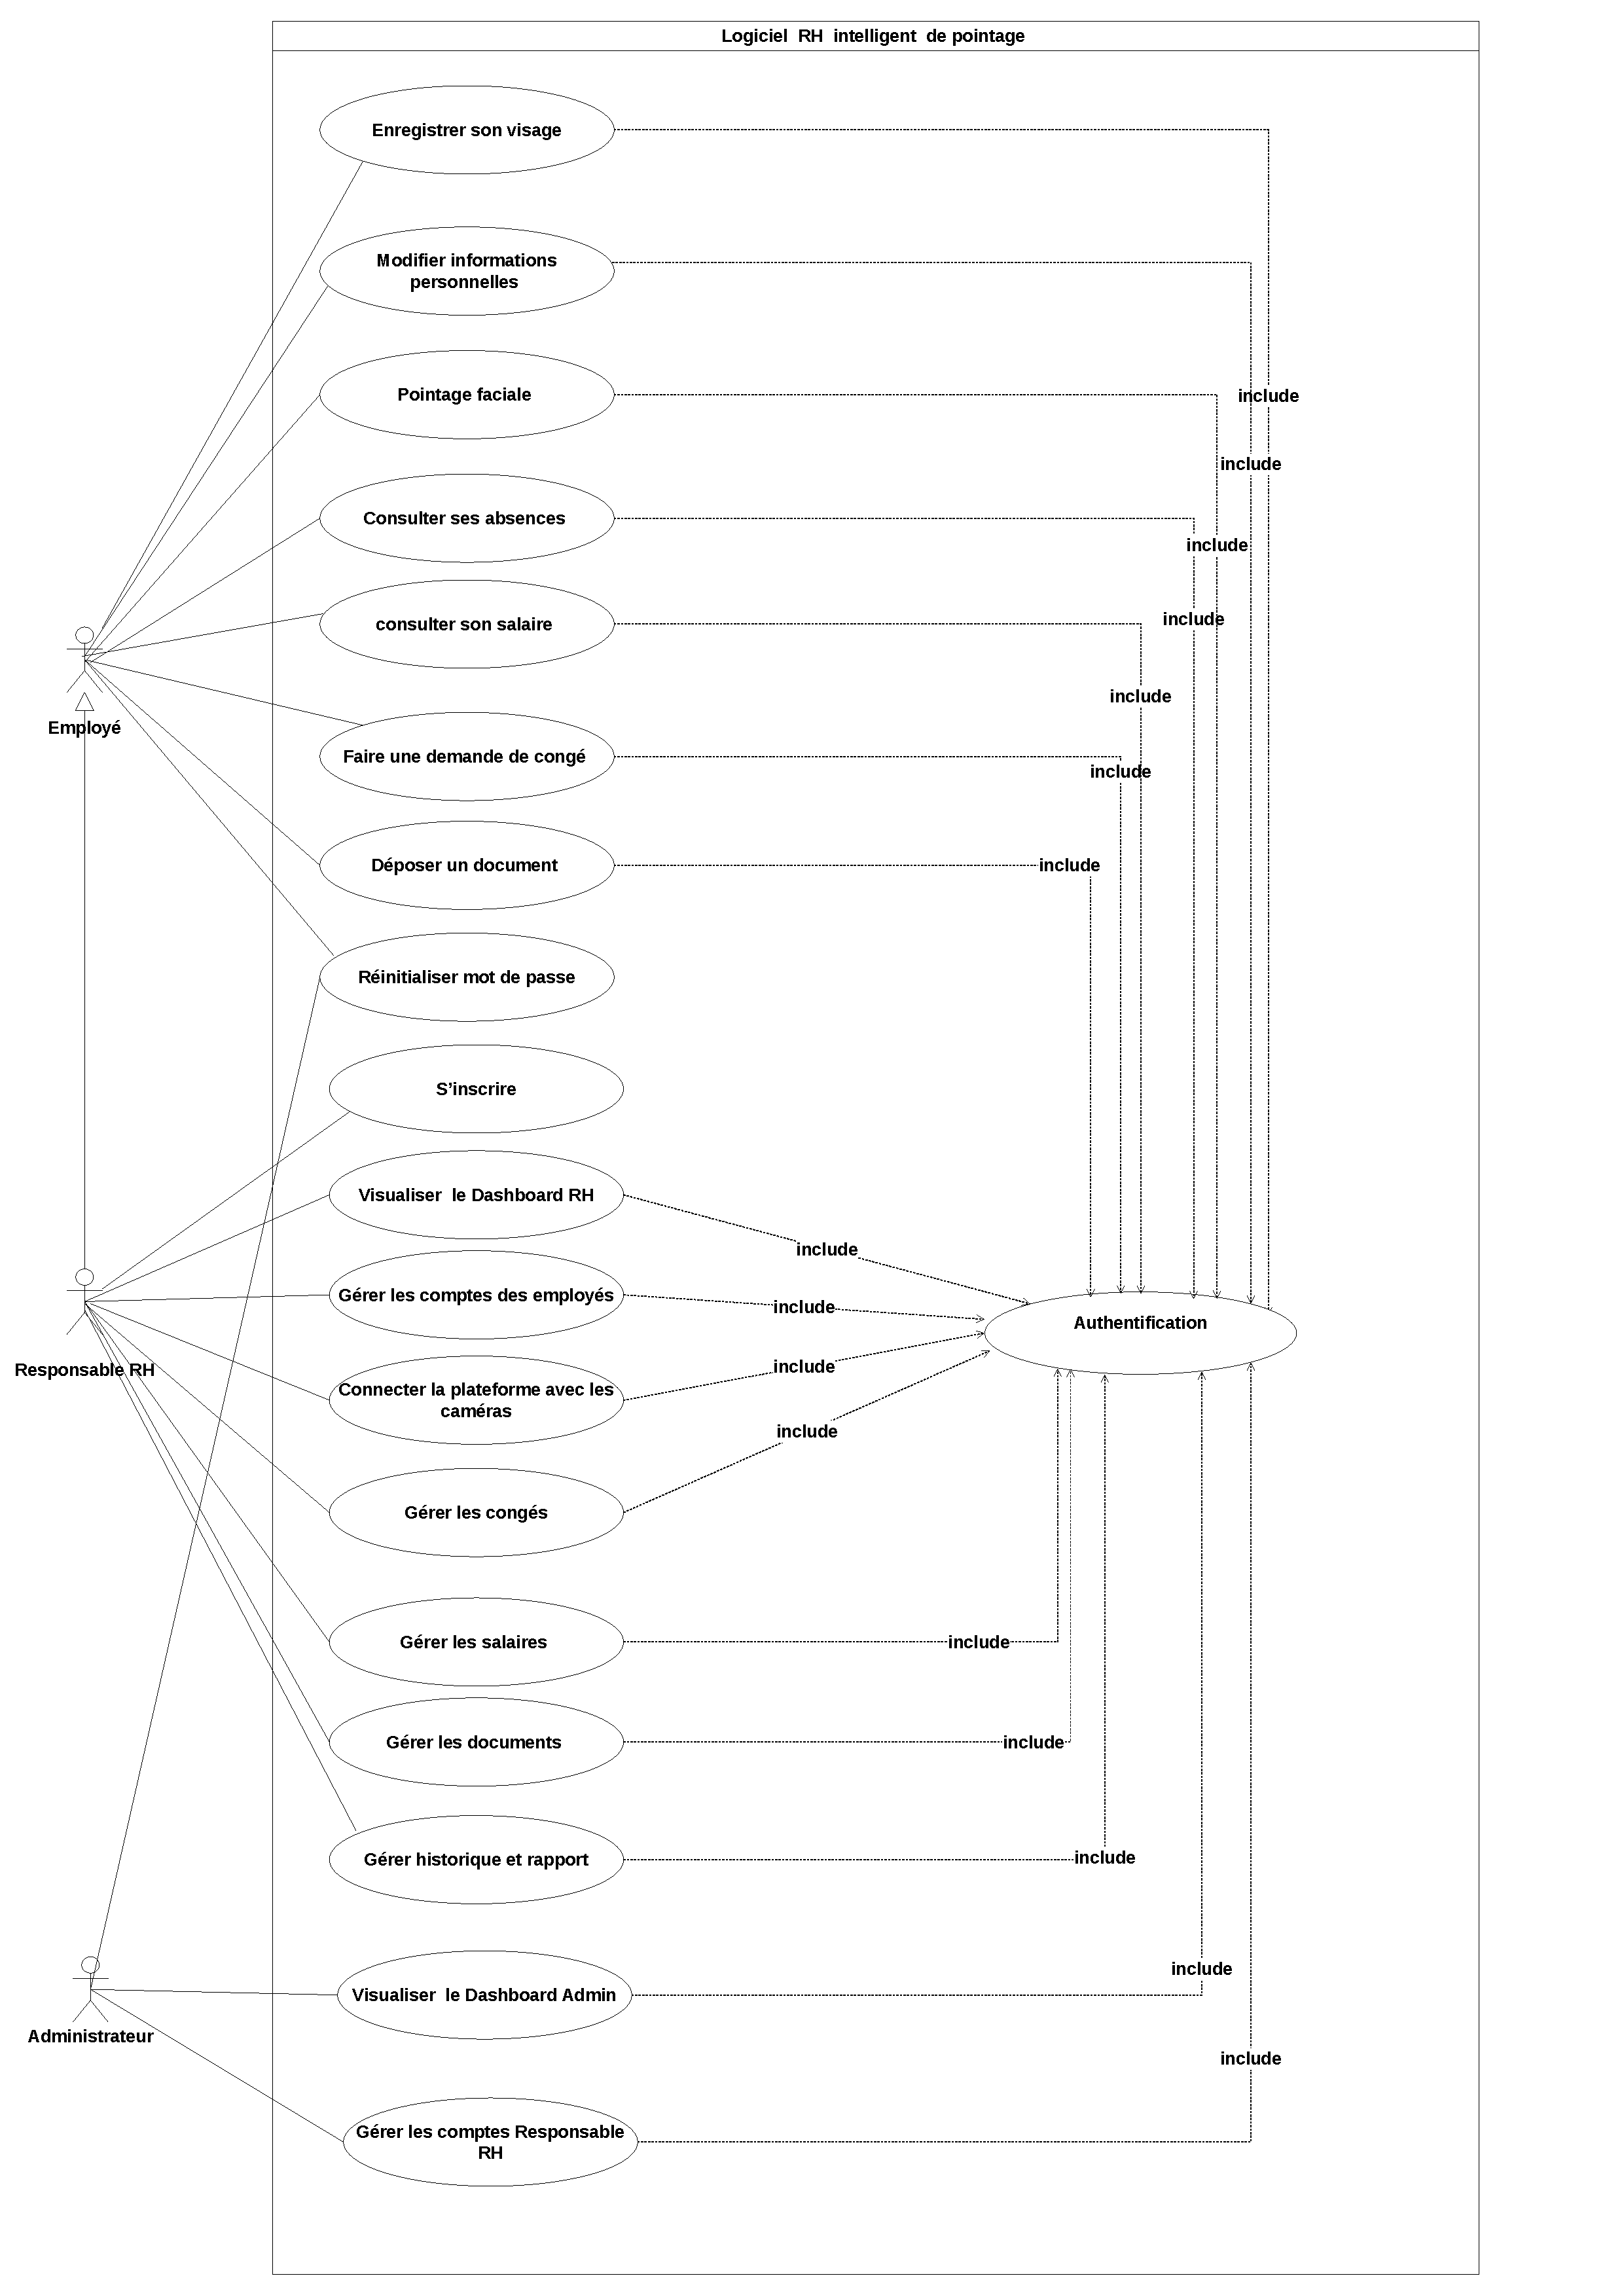
\includegraphics[
    width=0.8\paperwidth,
    height=1\textheight,
    keepaspectratio
  ]{projet/images/usecase/use.pdf}
  \caption{Diagramme de cas d'utilisation du système}
  \label{fig:usecase}
\end{figure}

\subsection{Besoins non fonctionnels}

Les besoins non fonctionnels définissent les contraintes et qualités attendues du système.

\begin{itemize}
  \item \textbf{Contraintes techniques :}
    \begin{itemize}
      \item Compatibilité avec les caméras standard.
      \item Temps de reconnaissance inférieur à 2 secondes.
      \item Base de données sécurisée et performante.
    \end{itemize}

  \item \textbf{Contraintes de sécurité :}
    \begin{itemize}
      \item Chiffrement des données sensibles.
      \item Authentification et autorisation des utilisateurs.
      
    \end{itemize}

  \item \textbf{Contraintes ergonomiques et esthétiques :}
    \begin{itemize}
      \item Interface intuitive et facile à utiliser.
      \item Navigation simple entre les fonctionnalités.
      \item Tableau de bord clair et lisible avec indicateurs visuels.
      \item Respect de l'identité visuelle de l'application et cohérence graphique.
    \end{itemize}
\end{itemize}

%============================================================
\section{Pilotage de projet avec Scrum}
%============================================================

Cette section présente l'application de la méthode Scrum dans le cadre du projet, en
détaillant l'organisation de l'équipe, la gestion du backlog ainsi que la planification
des différentes releases.

\subsection{Affectation des rôles Scrum}

L'équipe Scrum se compose de trois rôles différents, qui sont le Product Owner, le Scrum
Master et les développeurs. À chaque sprint, l'équipe Scrum est responsable de la création
d'un incrément de valeur à destination des utilisateurs et des clients.

Les rôles Scrum sont affectés comme suit :

\begin{itemize}
  \item \textbf{Product Owner :} BelHadj Mohamed
  \item \textbf{Scrum Master :} Amara Hiba
  \item \textbf{Développeurs :} Araar Mohamed et Mejri Louay
\end{itemize}

\subsection{Le Backlog de produit}

Le backlog du produit liste toutes les fonctionnalités, les exigences, les améliorations et
les correctifs à apporter à l'application à réaliser. Les différentes User Stories qui
composent le Backlog du produit représentent les objectifs à atteindre par l'équipe Scrum.
Le tableau~\ref{tab:backlog} illustre le backlog du produit du système à réaliser. Les
différentes user stories du backlog du produit sont ordonnées du plus prioritaires au moins
prioritaires. Les fonctionnalités prioritaires sont considérées comme indispensables pour le
système à mettre en œuvre, ces dernières permettant d'obtenir un produit qui contient le
minimum de fonctionnalités nécessaires pour être utilisé.

Une user story est souvent présentée de la manière suivante :
\og{}\textit{utilisateur + besoin + finalité}\fg{} avec

Le sprint backlog du projet et présenté par le tableau suivant :

\renewcommand{\arraystretch}{1.5}

\begin{longtable}{|>{\centering\arraybackslash}m{0.5cm}|
    >{\centering\arraybackslash}m{3cm}|
    >{\centering\arraybackslash}m{2.5cm}|
    >{\centering\arraybackslash}m{3cm}|
    >{\centering\arraybackslash}m{3cm}|
    >{\centering\arraybackslash}m{0.7cm}|
    >{\centering\arraybackslash}m{0.9cm}|}
\hline
\textbf{ID} & \textbf{User Story} & \textbf{En tant que} & \textbf{Je veux} &
\textbf{Afin de} & \textbf{P} & \textbf{C} \\
\hline
\endfirsthead
\hline
\textbf{ID} & \textbf{User Story} & \textbf{En tant que} & \textbf{Je veux} &
\textbf{Afin de} & \textbf{P} & \textbf{C} \\
\hline
\endhead

1  & Créer compte responsable RH    & Administrateur & créer un compte responsable RH    & administrer la plateforme        & 5 & 2 \\ \hline
2  & Modifier compte responsable RH & Administrateur & modifier un compte responsable RH & administrer la plateforme        & 4 & 2 \\ \hline
3  & Supprimer compte responsable RH& Administrateur & supprimer un compte responsable RH& administrer la plateforme        & 4 & 2 \\ \hline
4  & Visualiser le Dashboard Admin  & Administrateur & surveiller le fonctionnement global & assurer la stabilité du système & 5 & 4 \\ \hline
5  & S'inscrire                     & Responsable RH & créer mon compte sur la plateforme & accéder au système de gestion RH & 5 & 2 \\ \hline
6  & Visualiser le Dashboard RH     & Responsable RH & visualiser les indicateurs RH globaux & piloter l'activité RH         & 5 & 3 \\ \hline
7  & Créer compte employé           & Responsable RH & créer un compte employé           & permettre l'accès au système     & 5 & 2 \\ \hline
8  & Modifier compte employé        & Responsable RH & modifier un compte employé        & mettre à jour les informations et les accès de l'employé & 4 & 2 \\ \hline
9  & Supprimer compte employé       & Responsable RH & supprimer un compte employé       & désactiver définitivement l'accès de l'employé au système & 4 & 2 \\ \hline
10 & Connecter la plateforme aux caméras & Responsable RH & configurer et connecter les caméras & activer le pointage automatique & 5 & 5 \\ \hline
11 & Valider congé                  & Responsable RH & valider une demande de congé      & autoriser l'absence              & 5 & 2 \\ \hline
12 & Refuser congé                  & Responsable RH & refuser une demande de congé      & gérer les absences               & 5 & 2 \\ \hline
13 & Attribuer prime                & Responsable RH & attribuer une prime à un employé  & récompenser les employés         & 3 & 2 \\ \hline
14 & Attribuer déduction            & Responsable RH & appliquer une déduction à un employé & gérer la paie avec précision  & 4 & 3 \\ \hline
15 & Mettre à jour statut salaire   & Responsable RH & mettre à jour le statut du salaire & assurer la paie                 & 5 & 3 \\ \hline
16 & Consulter documents            & Responsable RH & consulter les documents envoyés   & vérifier les pièces              & 3 & 2 \\ \hline
17 & Valider document               & Responsable RH & approuver un document             & contrôler les absences           & 4 & 2 \\ \hline
18 & Rejeter document               & Responsable RH & refuser un document               & contrôler les absences           & 4 & 2 \\ \hline
19 & Modifier salaire               & Responsable RH & ajouter un salaire à un employé   & assurer une gestion correcte de la paie & 3 & 3 \\ \hline
20 & Générer rapport               & Responsable RH & générer un rapport                & exploiter les données RH         & 3 & 3 \\ \hline
21 & Consulter historique        & Responsable RH & consulter l'historique des actions effectuées & assurer le suivi et la traçabilité des opérations RH & 4 & 3 \\ \hline

22 & Enregistrer le visage          & Employé        & enregistrer mon visage            & permettre le pointage automatique & 5 & 5 \\ \hline
23 & Modifier infos personnelles    & Employé        & modifier mes informations personnelles & maintenir mes données à jour & 3 & 2 \\ \hline
24 & Consulter ses absences         & Employé        & consulter mes absences            & suivre ma présence               & 3 & 2 \\ \hline
25 & Consulter ses primes           & Employé        & consulter mes primes              & connaître mes avantages          & 2 & 1 \\ \hline
26 & Consulter déduction            & Employé        & voir mes déductions               & comprendre ma fiche de paie      & 2 & 1 \\ \hline
27 & Consulter son salaire          & Employé        & voir le statut de mon salaire     & savoir s'il est versé            & 3 & 1 \\ \hline
28 & Soumettre un congé             & Employé        & envoyer une demande de congé      & obtenir une autorisation d'absence & 5 & 2 \\ \hline
29 & Déposer un document            & Employé        & déposer un document               & justifier une absence            & 4 & 3 \\ \hline
30 & Pointage faciale               & Employé        & pointer ma présence par reconnaissance faciale & automatiser le pointage et éviter les oublis de pointage & 5 & 5 \\ \hline
31 & S'authentifier                 & Employé + Responsable RH + Administrateur & me connecter et me déconnecter    & accéder à mon espace sécurisé    & 5 & 2 \\ \hline

\caption{Backlog de produit}
\label{tab:backlog}
\end{longtable}

\subsection{Planification de releases}

À partir du product backlog défini en amont, le travail a été organisé selon une approche agile basée sur des cycles courts et itératifs. Chaque user story a été priorisée en fonction de sa valeur métier et de ses dépendances techniques, afin de déterminer un ordre d’exécution cohérent et optimal. En prenant en compte la taille de l’équipe ainsi qu’un calendrier global de quatre mois, la planification a été structurée en quatre sprints , couvrant la période du 14 février 2026 au 29 mai 2026. Les fonctionnalités essentielles, notamment la gestion des accès, l’administration des comptes et le pointage intelligent par reconnaissance faciale, ont été planifiées en priorité afin de garantir des fondations techniques robustes dès les premières itérations. L’ensemble des sprints est organisé en deux releases complémentaires, permettant une livraison progressive et maîtrisée du système.

\subsubsection*{Release 1 : Fondations \& Présence Intelligente}

La première release, du 14/02/2026 au 06/04/2026, regroupe les deux premiers sprints et constitue la base fonctionnelle du système. Elle couvre la gestion des accès, l’authentification sécurisée, l’administration des comptes ainsi que la mise en place du pointage intelligent par reconnaissance faciale. Cette phase permet de stabiliser l’architecture et de valider les fonctionnalités essentielles.
La répartition des user stories est détaillée dans le tableau suivant :
\begin{longtable}{|c|>{\raggedright\arraybackslash}p{4.2cm}|
    >{\centering\arraybackslash}p{2.5cm}|
    >{\centering\arraybackslash}p{3.5cm}|
    >{\raggedright\arraybackslash}p{5.5cm}|}
\hline
\textbf{ID} & \textbf{Nom Sprint} & \textbf{Story ID} & \textbf{Durée} & \textbf{Objectif} \\
\hline
\endfirsthead
\hline
\textbf{ID} & \textbf{Nom Sprint} & \textbf{Story ID} & \textbf{Durée} & \textbf{Objectif} \\
\hline
\endhead
1 & Gestion des Accès et Administration des Comptes
  & 1-2-3-5-7-8-9-31
  & 14/02/2026 -- 11/03/2026
  & Mettre en place l'authentification du système, la gestion des comptes
    (Administrateur, Responsable RH et Employé), la réinitialisation du mot de
    passe ainsi que le contrôle d'accès sécurisé à la plateforme. \\ \hline
2 & Pointage Intelligent et Suivi de Présence
  & 10-22-23-24-30
  & 12/03/2026 -- 06/04/2026
  & Implémenter le pointage automatique par reconnaissance faciale, connecter
    les caméras et permettre le suivi des présences, absences et informations
    personnelles des employés. \\ \hline
\caption{Release 1}
\end{longtable}

\subsubsection*{Release 2 : Gestion RH Complète et Pilotage}
La deuxième release, du 07/04/2026 au 29/05/2026, regroupe les sprints suivants et introduit les fonctionnalités avancées. Elle inclut la gestion des congés, des documents administratifs et de la paie, ainsi que les modules de reporting, de traçabilité et de pilotage RH via tableaux de bord. Cette phase finalise le système en enrichissant ses capacités fonctionnelles et décisionnelles.
La répartition des user stories est détaillée dans le tableau suivant :
\begin{longtable}{|c|>{\raggedright\arraybackslash}p{4.2cm}|
    >{\centering\arraybackslash}p{2.5cm}|
    >{\centering\arraybackslash}p{3.5cm}|
    >{\raggedright\arraybackslash}p{5.5cm}|}
\hline
\textbf{ID} & \textbf{Nom Sprint} & \textbf{Story ID} & \textbf{Durée} & \textbf{Objectif} \\
\hline
\endfirsthead

3 & Gestion  des Congés et des Documents Administratifs
  & 11-12-13-14-15-16-17-18-19-25-26-27-28-29
  & 07/04/2026 -- 02/05/2026
  & Développer les fonctionnalités liées à la gestion des congés, documents,
    primes, déductions et salaires, ainsi que la validation, le rejet et le
    dépôt des documents administratifs. \\ \hline
4 & Pilotage RH, Reporting et Traçabilité
  & 4-6-20-21
  & 03/05/2026 -- 29/05/2026
  & Implémenter les tableaux de bord (Administrateur et Responsable RH),
    la génération des rapports, la consultation de l'historique des actions
    RH. \\ \hline
\caption{Release 2}
\end{longtable}

\subsection{Diagramme de Gantt}

Ce diagramme montre la planification temporelle du projet en illustrant l'organisation des
sprints, des tâches et des différentes phases de développement du système RH intelligent.

\begin{figure}[H]
  \centering
  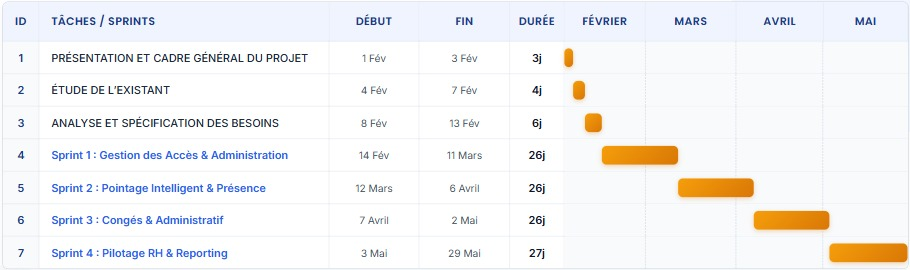
\includegraphics[width=\textwidth]{projet/images/daigramme_de_gant.jpeg}
  \caption{Diagramme de Gantt du projet}
  \label{fig:gantt}
\end{figure}

%============================================================
\section{Étude technique}
%============================================================

Cette étude technique a pour but d'analyser en détail les différentes composantes et
mécanismes impliqués dans notre logiciel.

\subsection{Environnement matériel}

La réalisation de notre projet utilise deux machines de caractéristiques différentes :

\begin{table}[H]
\centering
\renewcommand{\arraystretch}{1.5}
\begin{tabular}{|p{5cm}|p{8cm}|}
\hline
\textbf{Marque}              & Dell Latitude 5530 \\ \hline
\textbf{Mémoire}             & 24,0 Go \\ \hline
\textbf{Processeur}          & 12th Gen Intel(R) Core(TM) i5-1245U (1.60 GHz) \\ \hline
\textbf{Disque dur}          & 725 Go \\ \hline
\textbf{Système d'exploitation} & Windows 11 Professionnel \\ \hline
\end{tabular}
\caption{Environnement matériel 1}
\end{table}

\begin{table}[H]
\centering
\renewcommand{\arraystretch}{1.5}
\begin{tabular}{|p{5cm}|p{8cm}|}
\hline
\textbf{Marque}              & Dell vostro 3530  \\ \hline
\textbf{Mémoire}             & 16,0 Go \\ \hline
\textbf{Processeur}          & AMD Ryzen 7 5700U with Radeon Graphics \\ \hline
\textbf{Disque dur}          & 1 To \\ \hline
\textbf{Système d'exploitation} & Windows 11 Professionnel \\ \hline
\end{tabular}
\caption{Environnement matériel 2}
\end{table}

\subsection{Environnement logiciel}

Dans cette partie, nous détaillons l'ensemble des environnements logiciels utilisés dans
le cadre du projet, incluant les outils de conception, de développement, ainsi que les
langages, frameworks et bibliothèques employés.

\subsubsection{Logiciels de conception}

Lors de la conception de notre site, nous avons utilisé les logiciels suivants :

\begin{table}[H]
\centering
\renewcommand{\arraystretch}{1.5}
\begin{tabular}{|m{3cm}|m{10cm}|}
\hline
\centering
\vspace{0.2cm}

\includegraphics[height=2cm]{projet/images/Figma-logo.png}
&
\textbf{Figma :} Figma est un outil de conception d'interfaces graphiques permettant de
créer, partager et tester des designs pour les sites web, les applications mobiles et
d'autres produits numériques. Il facilite également la collaboration en temps réel entre
les membres d'une équipe.\cite{figma}
\\ \hline
\centering
\vspace{0.2cm}

\includegraphics[height=2cm]{projet/images/ps adobe.png}
&
\textbf{Adobe Photoshop :} Adobe Photoshop est un logiciel de retouche et de traitement
d'images numériques. Il permet la modification, la création et l'amélioration des images
et des supports graphiques professionnels.\cite{photoshop}
\\ \hline
\centering
\vspace{0.2cm}

\includegraphics[height=2cm]{projet/images/draw io.png}
&
\textbf{draw.io :} draw.io est un outil de création de diagrammes en ligne permettant de
réaliser des organigrammes, des diagrammes UML, des schémas réseau et d'autres
représentations graphiques de manière simple et efficace.\cite{drawio}
\\ \hline

\centering
\vspace{0.2cm}

\includegraphics[height=2cm]{projet/images/overlef.png}
&
\textbf{Overleaf :}  outil de rédaction de documents scientifiques en LaTeX
en ligne, utilisé pour la rédaction et la mise en forme du rapport de
stage.\cite{overleaf}
\\ \hline

\end{tabular}
\caption{Environnement logiciel de conception}
\end{table}

\subsubsection{Logiciels de développement}

Lors du développement de notre site, nous avons utilisé les logiciels suivants :

\begin{table}[H]
\centering
\renewcommand{\arraystretch}{1.4}
\begin{tabular}{|m{3cm}|m{10cm}|}
\hline
\centering
\vspace{0.2cm}
\includegraphics[height=2cm]{projet/images/vs.jpeg}
&
\textbf{Visual Studio Code :} VSCode est un éditeur de code source et un IDE open-source
compatible avec Windows, Linux et Mac.\cite{Visual Studio Code}
\\ \hline
\centering
\vspace{0.2cm}
\includegraphics[height=2cm]{projet/images/tt.jpeg}
&
\textbf{GitHub :} GitHub est un service cloud qui nous aide à stocker et gérer le code,
à suivre et contrôler les modifications.\cite{GitHub}
\\ \hline
\centering
\vspace{0.2cm}
\includegraphics[height=2cm]{projet/images/postamn.jpeg}
&
\textbf{Postman :} Postman est un outil de développement et de test d'API qui permet
d'envoyer des requêtes HTTP (GET, POST, PUT, DELETE…), d'analyser les réponses du
serveur et de vérifier le bon fonctionnement des services web.\cite{Postman}
\\ \hline
\end{tabular}
\caption{Environnement logiciel de développement}
\end{table}

\subsubsection{Langages de développement}

Lors du développement de notre site, nous avons utilisé les langages suivants :

\renewcommand{\arraystretch}{1.4}
\setlength{\LTleft}{\fill}
\setlength{\LTright}{\fill}
\begin{longtable}{|m{14cm}|}
\hline
\textbf{HTML :} HTML (HyperText Markup Language) est le langage de base du Web qui
structure le contenu des pages.\cite{HTML} \\ \hline
\textbf{CSS :} CSS (Cascading Style Sheets) permet de définir la présentation visuelle
des pages web.\cite{CSS} \\ \hline
\textbf{JavaScript :} JavaScript (JS) est un langage de programmation léger interprété
(ou compilé juste-à-temps) avec des fonctions de première classe. Bien qu'il soit le
langage de script le plus connu pour les pages Web, il est utilisé pour les interactions
dynamiques et les animations.\cite{JavaScript} \\ \hline
\textbf{TypeScript :} Extension de JavaScript utilisée pour améliorer la fiabilité et
la maintenance du code.\cite{TypeScript} \\ \hline
\textbf{Python :} Langage utilisé pour développer le modèle de reconnaissance faciale
et le serveur backend.\cite{Python} \\ \hline
\textbf{SQL :} Langage utilisé pour gérer la base de données.\cite{SQL} \\ \hline
\caption{Langages de développement}
\end{longtable}

\subsubsection{Frameworks et bibliothèques}

Lors du développement de notre site, nous avons utilisé les frameworks et bibliothèques
suivants :

\begin{longtable}{|m{14cm}|}
\hline
\textbf{Next.js :} Framework React full-stack permettant de développer le frontend et
le backend dans une seule application.\cite{Next.js} \\ \hline
\textbf{React :} Bibliothèque JavaScript utilisée pour construire l'interface
utilisateur.\cite{React} \\ \hline
\textbf{Flask :} Micro-framework pour développer des applications web et des
API.\cite{Flask} \\ \hline
\textbf{OpenCV :} Bibliothèque de vision par ordinateur pour le traitement
d'images.\cite{OpenCV} \\ \hline
\textbf{MediaPipe :} Bibliothèque utilisée pour la détection des visages et des points
caractéristiques.\cite{MediaPipe} \\ \hline
\textbf{TensorFlow :} Bibliothèque d'apprentissage automatique utilisée pour
l'entraînement du modèle.\cite{TensorFlow} \\ \hline
\caption{Frameworks et bibliothèques}
\end{longtable}

%============================================================
\section{Architecture de la solution}
%============================================================

Dans cette section, nous présentons l'architecture logique et logicielle de notre système.

\subsection{Architecture logique}

L'architecture logique identifie les composants logiciels nécessaires à l'implémentation
d'une solution et décrit les relations existant entre ces composants. Notre logiciel RH
intelligent repose sur une architecture en trois tiers (\textit{3-tier architecture}),
permettant une séparation claire des responsabilités. Elle se compose d'une couche
présentation responsable de l'interface utilisateur, d'une couche métier contenant les
règles de gestion, et d'une couche d'accès aux données assurant la persistance des
informations. Cette structuration améliore la maintenabilité, la modularité et
l'évolutivité du système.

\begin{figure}[H]
  \centering
  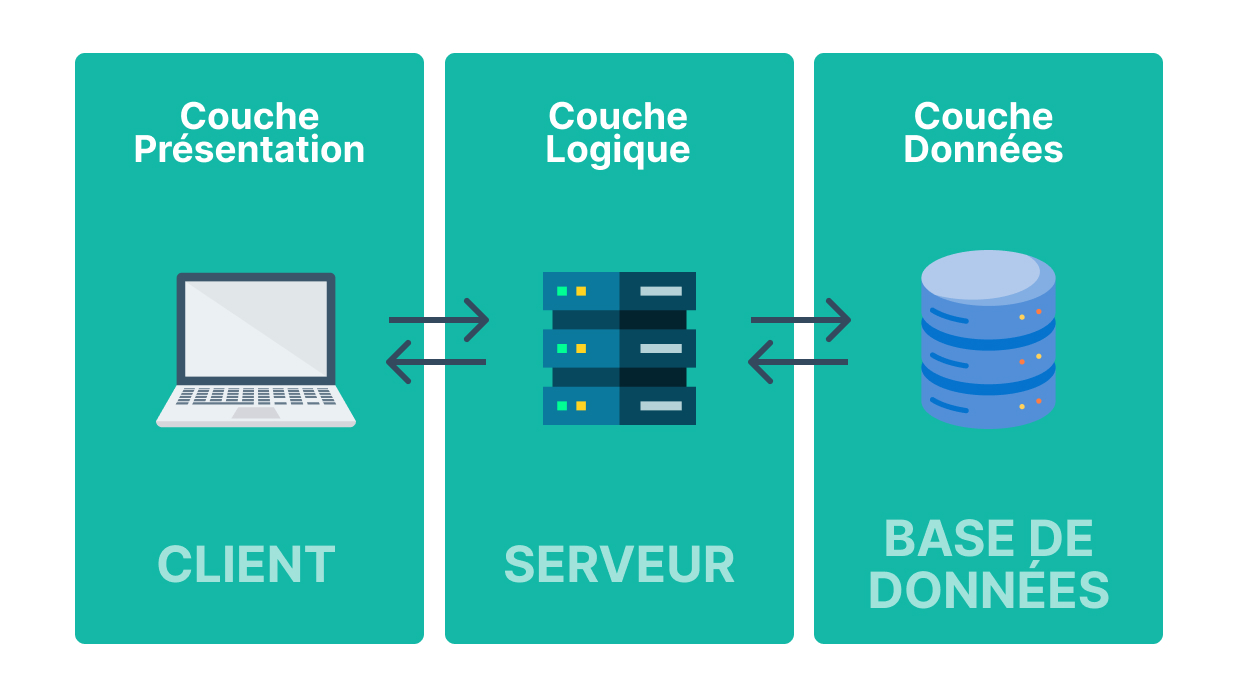
\includegraphics[scale=0.2]{projet/images/architecture logique.jpg}
  \caption{Architecture logique}
\end{figure}

\subsection{Architecture logicielle}

Le système adopte une \textbf{architecture logicielle découplée orientée API}, dans
laquelle chaque couche est développée de manière indépendante et communique avec les
autres exclusivement via des \textbf{interfaces REST}. Cette approche s'inscrit dans une
\textbf{architecture 3 tiers} en précisant l'organisation interne de chaque couche.

La \textbf{couche présentation} est assurée par \textbf{Next.js}, un framework React
qui offre un rendu hybride combinant le \textbf{rendu côté serveur (SSR)} et le
\textbf{rendu côté client (CSR)}, garantissant ainsi de bonnes performances et une
expérience utilisateur fluide. Elle communique avec le backend à travers des
\textbf{requêtes HTTP sécurisées} et adapte dynamiquement l'interface en fonction du
rôle de l'utilisateur.

La \textbf{couche métier} repose sur \textbf{Flask}, un framework Python léger et
flexible, permettant de développer des \textbf{API REST} de manière simple et efficace.
L'organisation du code est structurée de manière à assurer une \textbf{séparation claire
des responsabilités} et à faciliter la maintenance du système.

Le système intègre également un \textbf{module d'intelligence artificielle} dédié à la
\textbf{reconnaissance faciale}. Ce module est développé en \textbf{Python} et intégré
au backend Flask sous forme de \textbf{services spécialisés}. Il permet d'automatiser
certaines tâches comme le \textbf{pointage} ou la \textbf{vérification d'identité},
tout en restant \textbf{indépendant et évolutif}.

Enfin, la \textbf{couche de données} est assurée par \textbf{MySQL}, un système de
gestion de base de données relationnelle permettant de stocker et de gérer efficacement
les informations liées aux employés, aux congés et aux différentes opérations du système.

\begin{figure}[H]
  \makebox[\textwidth][l]{%
    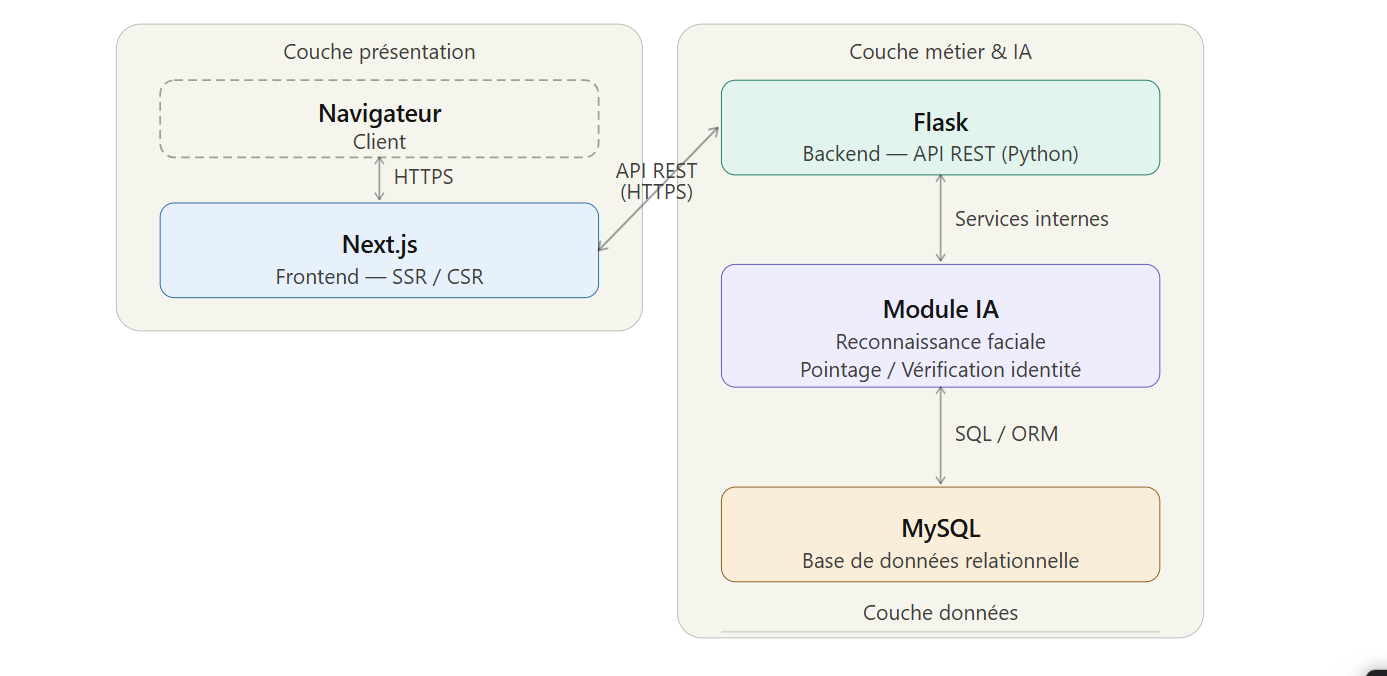
\includegraphics[width=0.9\textwidth]{projet/images/xc.png}
  }
  \caption{Architecture logicielle du système}
\end{figure}

%============================================================
\section{Conclusion}
%============================================================

Dans ce chapitre, nous avons abordé de manière détaillée les besoins fonctionnels et non
fonctionnels du projet, présenté l'environnement logiciel nécessaire à sa réalisation,
ainsi que les différents rôles Scrum impliqués. De plus, nous avons élaboré le product
backlog avec une répartition en releases. En conclusion, ce chapitre a posé les bases
essentielles pour la gestion efficace du projet. Le prochain chapitre se concentrera sur
le contenu spécifique de la première release, mettant en lumière les fonctionnalités clés
à développer pour répondre aux besoins identifiés.

\chapter{Release 1}

\newpage

%============================================================
\section{Introduction}
%============================================================

Ce chapitre est essentiel pour le déroulement du projet, puisqu'il présente en détail la première version du produit final, appelée Release~1. La sortie de cette version est très importante car elle rassemble les fonctionnalités essentielles de notre projet et est indispensable pour finaliser la deuxième partie des fonctionnalités.

%============================================================
\section{Sprint 1 : Gestion des Accès et Administration des Comptes}
%============================================================

Ce sprint a pour objectif de développer le module d'authentification et de gestion des comptes utilisateurs, ainsi que la réinitialisation de mot de passe, permettant un accès sécurisé à la plateforme selon les rôles définis (Administrateur, Responsable RH et Employé).

\subsection{Objectif du sprint 1}

L'objectif de ce sprint est d'implémenter l'authentification du système, la gestion des comptes (Administrateur, Responsable RH, Employé) et le contrôle d'accès sécurisé à la plateforme.

\subsection{Durée du sprint 1}

\begin{itemize}
    \item \textbf{Date de début du sprint} : 14/02/2026
    \item \textbf{Date de fin du sprint} : 11/03/2026
\end{itemize}

\subsection{Backlog du sprint 1}
Ce tableau présente les neuf user stories retenues pour le sprint 1, couvrant la gestion des comptes Administrateur, Responsable RH et Employé, ainsi que l'authentification et la réinitialisation du mot de passe. Chaque user story est accompagnée de sa priorité (P) et de sa complexité estimée (C).

sprint. Le sprint backlog du sprint 1 est présenté dans le tableau suivant :

\begin{longtable}{|>{\centering\arraybackslash}m{0.5cm}|
    >{\centering\arraybackslash}m{3cm}|
    >{\centering\arraybackslash}m{2.5cm}|
    >{\centering\arraybackslash}m{3cm}|
    >{\centering\arraybackslash}m{3cm}|
    >{\centering\arraybackslash}m{0.7cm}|
    >{\centering\arraybackslash}m{0.9cm}|}
\hline
\textbf{ID} & \textbf{User Story} & \textbf{En tant que} & \textbf{Je veux} & \textbf{Afin de} & \textbf{P} & \textbf{C} \\
\hline
\endfirsthead
\hline
\textbf{ID} & \textbf{User Story} & \textbf{En tant que} & \textbf{Je veux} & \textbf{Afin de} & \textbf{P} & \textbf{C} \\
\hline
\endhead
1  & Créer compte responsable RH    & Administrateur  & créer un compte responsable RH    & administrer la plateforme        & 5 & 2 \\ \hline
2  & Modifier compte responsable RH & Administrateur  & modifier un compte responsable RH & administrer la plateforme        & 4 & 2 \\ \hline
3  & Supprimer compte responsable RH& Administrateur  & supprimer un compte responsable RH& administrer la plateforme        & 4 & 2 \\ \hline
5  & S'inscrire                     & Responsable RH  & créer mon compte sur la plateforme& accéder au système de gestion RH & 5 & 2 \\ \hline
7  & Créer compte employé           & Responsable RH  & créer un compte employé           & permettre l'accès au système     & 5 & 2 \\ \hline
8  & Modifier compte employé        & Responsable RH  & modifier un compte employé        & mettre à jour les données        & 4 & 2 \\ \hline
9  & Supprimer compte employé       & Responsable RH  & supprimer un compte employé       & désactiver l'accès               & 4 & 2 \\ \hline
31 & S'authentifier                 & Employé + Responsable RH + Administrateur & me connecter et me déconnecter    & accéder à mon espace sécurisé    & 5 & 2 \\ \hline

\caption{Backlog Sprint 1 — Accès \& Identités}
\end{longtable}


\subsection{Spécification fonctionnelle détaillée}

\subsubsection*{Diagramme de cas d'utilisation du sprint 1}

Ce diagramme illustre les interactions entre les trois acteurs principaux — Administrateur, Responsable RH et Employé — et les fonctionnalités du sprint 1, notamment la gestion des comptes et l'authentification.
\begin{figure}[H]
    \centering
    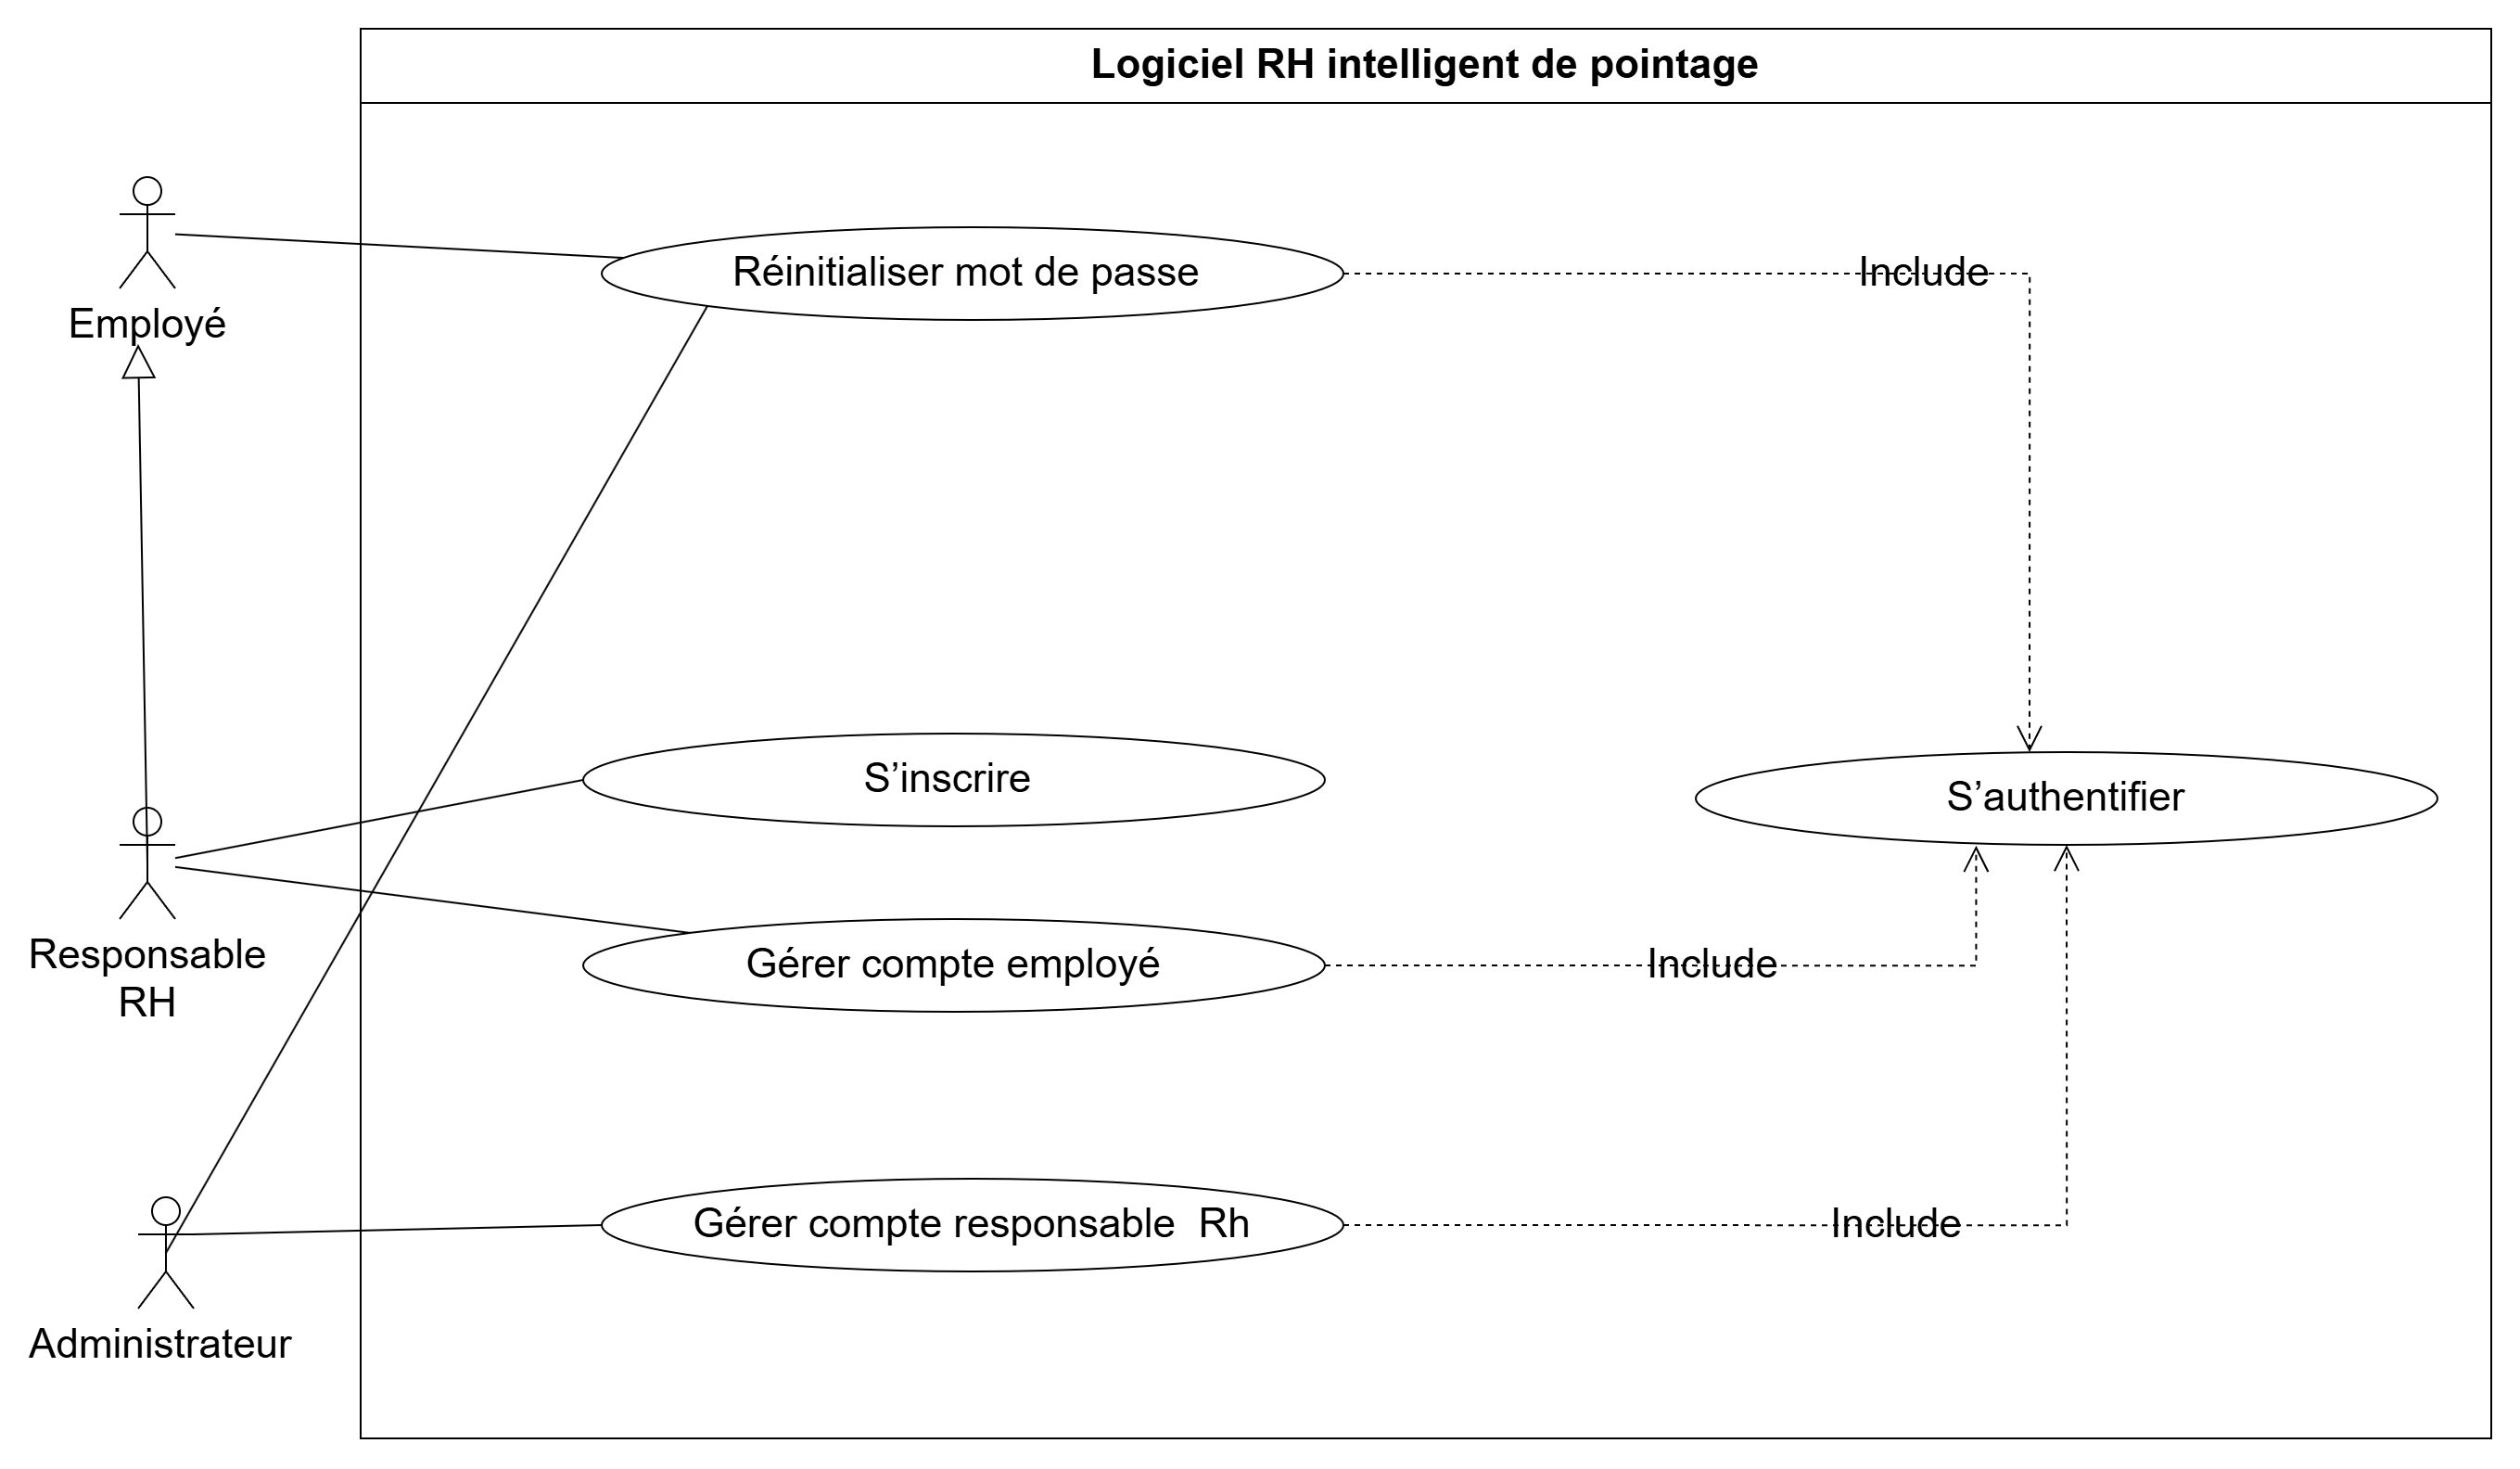
\includegraphics[width=0.9\textwidth]{projet/images/usecase/sprint1/use_case_sprint1.png}
    \caption{Diagramme de Cas d'utilisation du Sprint 1}
    \label{fig:usecase1}
\end{figure}







\subsubsection*{Description textuelle : cas d'utilisation « S'authentifier »}
Ce tableau présente le scénario d'authentification d'un utilisateur, depuis l'accès à la page de connexion jusqu'à la redirection vers le tableau de bord, ainsi que le cas d'exception lié à des identifiants invalides.
\begin{longtable}{|p{5cm}|p{11cm}|}
\hline
\textbf{Nom du cas d'utilisation} & \textbf{S'authentifier} \\ \hline
\textbf{Acteurs}                  & Utilisateur \\ \hline
\textbf{Objectif}                 & Permettre à l'utilisateur d'accéder au système \\ \hline
\textbf{Préconditions}            & L'utilisateur possède un compte valide \\ \hline
\textbf{Scénario nominal} &
1. L'utilisateur accède à la page de connexion. \newline
2. Le système affiche le formulaire de connexion . \newline
3. L'utilisateur saisit son login et son mot de passe  \newline
4. L'utilisateur clique sur « Se connecter ». \newline
5. Le système envoie les identifiants pour vérification. \newline
6. Le système valide les identifiants. \newline
7. Le système affiche le tableau de bord. \newline
8. L'utilisateur est redirigé avec succès. \\ \hline
\textbf{Scénario d'exception} &
1.1 Si les identifiants sont invalides : \newline
Le système affiche un message d'erreur. \\ \hline
\textbf{Post-condition} & L'utilisateur est connecté et accède à son tableau de bord \\ \hline
\caption{Description textuelle du cas d'utilisation « S'authentifier »}
\end{longtable}



\subsubsection*{Description textuelle : cas d'utilisation « S'inscrire »}
Ce tableau détaille le processus d'inscription d'un nouveau Responsable RH, en présentant les étapes de saisie des informations, de vérification par le système et de création du compte, ainsi que le scénario d'exception en cas d'échec.

\begin{longtable}{|p{5cm}|p{11cm}|}
\hline
\textbf{Nom du cas d'utilisation} & \textbf{S'inscrire} \\ \hline
\textbf{Acteurs}                  & Responsable RH \\ \hline
\textbf{Objectif}                 & Permettre à un nouvel utilisateur de créer un compte sur la plateforme \\ \hline
\textbf{Préconditions}            & L'utilisateur ne possède pas encore de compte \\ \hline
\textbf{Scénario nominal} &
1. L'utilisateur accède à la page d'inscription. \newline
2. L'utilisateur saisit les informations demandées . \newline
3. Le système vérifie les informations reçues. \newline
4. Le système enregistre les informations dans la base de données. \newline
5. L'utilisateur est redirigé vers son tableau de bord. \\ \hline
\textbf{Scénario d'exception} &
5.1 Si les informations sont invalides ou l'inscription échoue, le système affiche un message d'erreur et demande de réessayer. \\ \hline
\textbf{Post-condition} & Un nouveau compte utilisateur est créé et l'utilisateur peut accéder à la plateforme. \\ \hline
\caption{Description textuelle du cas d'utilisation « S'inscrire »}
\end{longtable}


\subsubsection*{Raffinement du cas d'utilisation « Gérer compte employé »}
Ce diagramme raffine le cas d'utilisation « Gérer compte employé » en décomposant les trois opérations possibles : la création, la modification et la suppression d'un compte employé par le Responsable RH.

\begin{figure}[H]
    \centering
    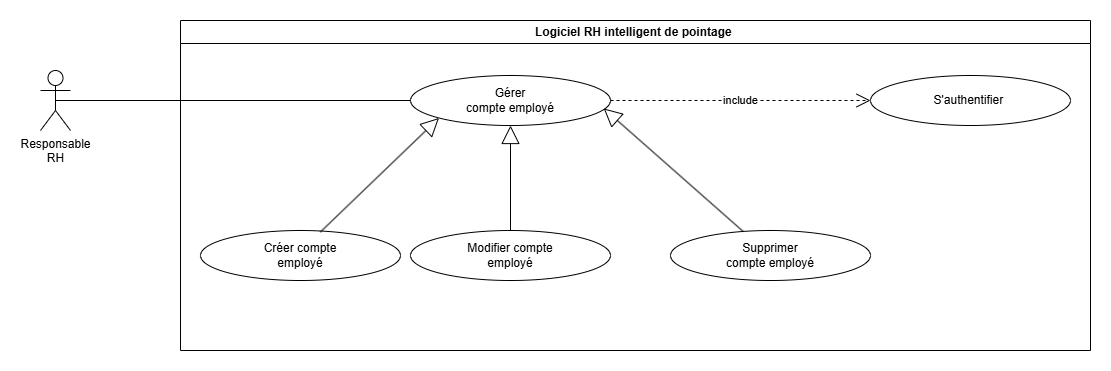
\includegraphics[width=0.9\textwidth]{projet/images/usecase/sprint1/gerer_compte_employe.png}
    \caption{Raffinement du cas d'utilisation « Gérer compte employé »}
    \label{fig:usecase2}
\end{figure}


\subsubsection*{Description textuelle : cas d'utilisation « Gérer compte employé »}
Ce tableau décrit les scénarios de création, modification et suppression d'un compte employé, incluant le processus d'envoi d'un lien d'activation par e-mail et les exceptions liées à des données invalides.

\begin{longtable}{|p{5cm}|p{11cm}|}
\hline
\textbf{Nom du cas d'utilisation} & \textbf{Gérer compte employé} \\ \hline
\textbf{Acteurs}                  & Responsable RH \\ \hline
\textbf{Objectif}                 & Créer, modifier et supprimer un compte employé \\ \hline
\textbf{Préconditions}            & Responsable RH authentifié et compte employé existant ou en cours de création \\ \hline
\textbf{Scénario nominal} &
\textbf{Création :} \newline
1. Le Responsable RH accède à la gestion des employés. \newline
2. Il clique sur « Ajouter employé ». \newline
3. Il saisit les informations de l'employé. \newline
4. Il valide la création. \newline
5. Le système crée le compte. \newline
6. Le système envoie un email contenant un lien de définition du mot de passe. \newline
7. L'employé clique sur le lien reçu par email. \newline
8. Il définit son mot de passe pour activer son compte. \newline
\textbf{Modification :} \newline
9. Le Responsable RH accède à la liste des employés. \newline
10. Il sélectionne un employé. \newline
11. Il clique sur « Modifier compte ». \newline
12. Le Responsable RH fait des modifications. \newline
13. Le système met à jour le compte. \newline
\textbf{Suppression :} \newline
14. Le Responsable RH accède à la liste des employés. \newline
15. Il sélectionne un employé. \newline
16. Il clique sur « Supprimer compte ». \newline
17. Le système supprime le compte de l'employé. \\ \hline
\textbf{Scénario d'exception} &
3.1 Si les données sont invalides, le système affiche une erreur. \newline
12.1 Si les données modifiées sont invalides, le système affiche une erreur. \\ \hline
\textbf{Post-condition} & Le compte employé est créé, modifié ou supprimé selon l'action effectuée. \\ \hline
\caption{Description textuelle du cas d'utilisation « Gérer compte employé »}
\end{longtable}


\subsubsection*{Raffinement du cas d'utilisation « Gérer compte Responsable RH »}
Ce diagramme raffine le cas d'utilisation « Gérer compte Responsable RH » en illustrant les actions de création, modification et suppression d'un compte Responsable RH effectuées par l'Administrateur.

\begin{figure}[H]
    \centering
    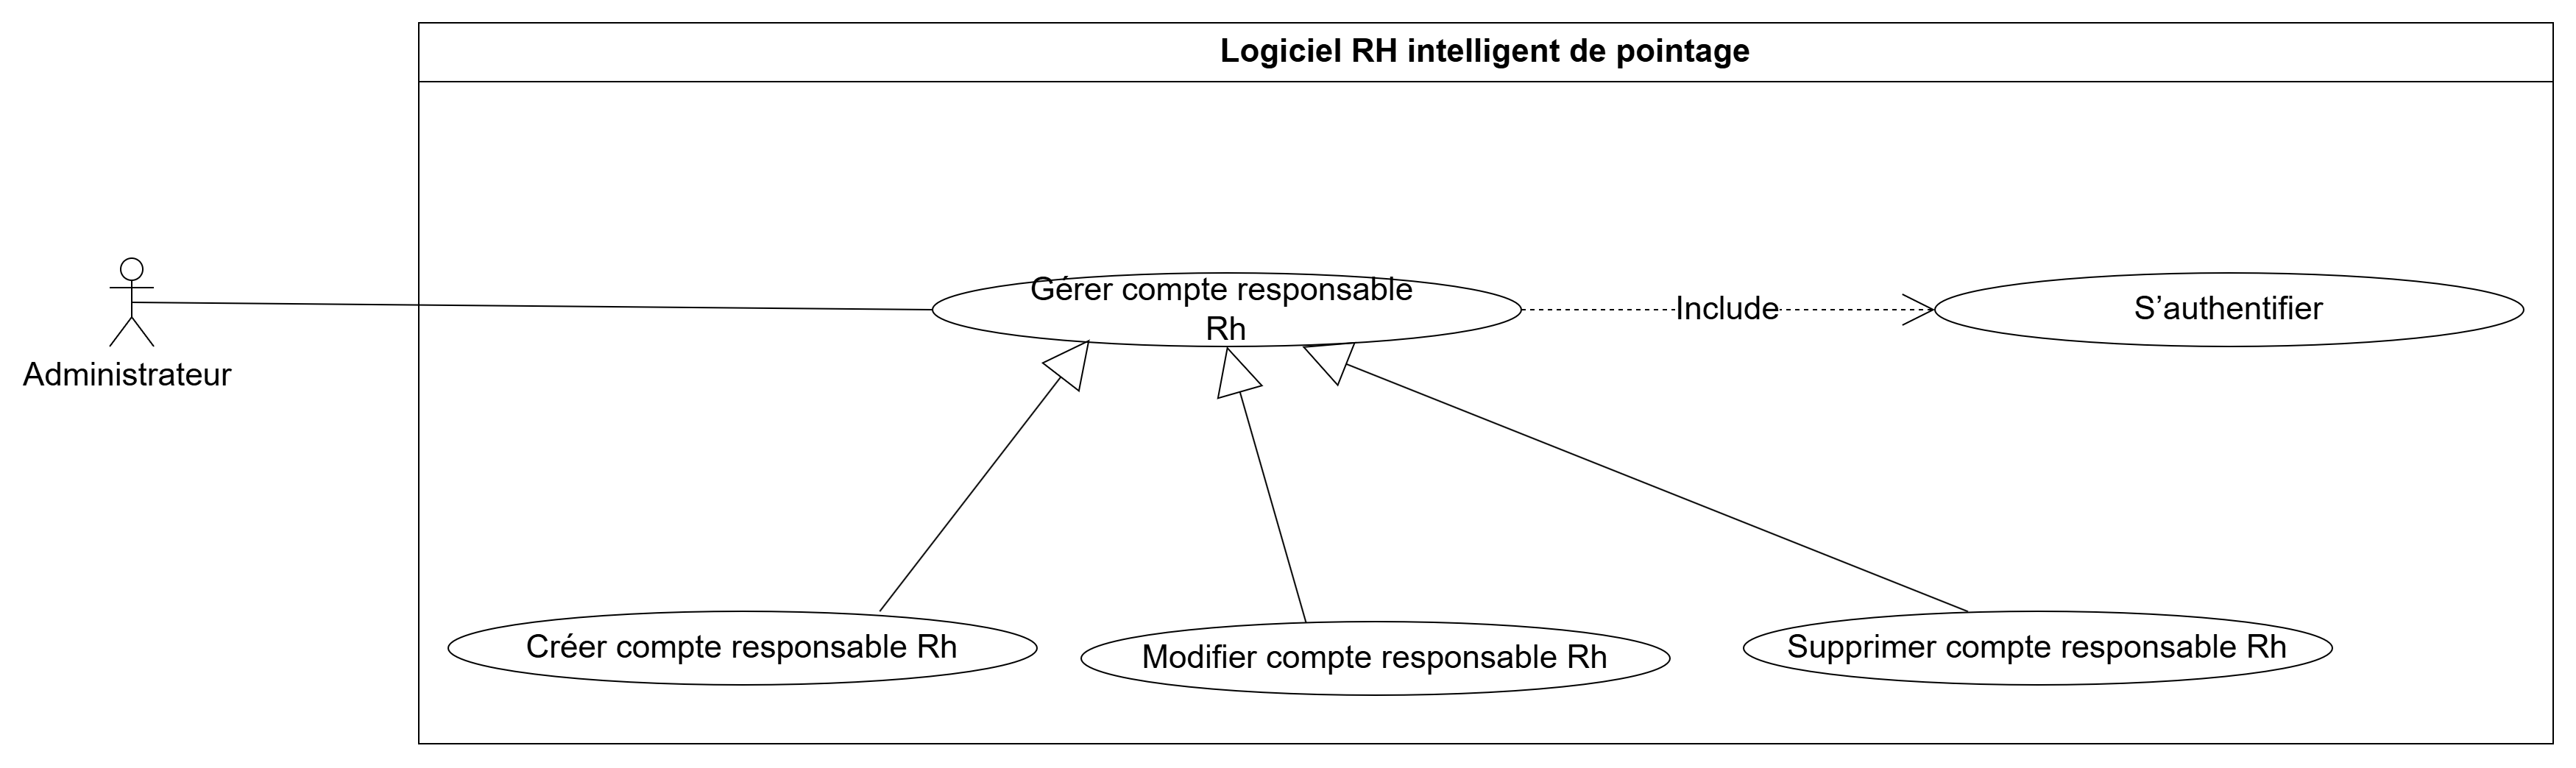
\includegraphics[width=0.9\textwidth]{projet/images/usecase/sprint1/gere_compte_rh.png}
    \caption{Raffinement du cas d'utilisation « Gérer compte Responsable RH »}
    \label{fig:usecase3}
\end{figure}


\subsubsection*{Description textuelle : cas d'utilisation « Gérer compte Responsable RH »}
Ce tableau présente les étapes détaillées de gestion d'un compte Responsable RH par l'Administrateur, avec les scénarios d'exception associés, notamment la vérification des doublons lors de la création et la demande de confirmation avant suppression.

\begin{longtable}{|p{5cm}|p{11cm}|}
\hline
\textbf{Nom du cas d'utilisation} & \textbf{Gérer compte Responsable RH} \\ \hline
\textbf{Acteurs}                  & Administrateur \\ \hline
\textbf{Objectif}                 & Créer, modifier et supprimer un compte Responsable RH \\ \hline
\textbf{Préconditions}            & L'administrateur doit être authentifié \\ \hline
\textbf{Scénario nominal} &
\textbf{Création :} \newline
1. L'administrateur accède à l'interface de gestion utilisateur. \newline
2. L'administrateur clique sur « Ajouter un compte RH ». \newline
3. L'administrateur saisit les informations nécessaires (nom, nom entreprise, email, mot de passe). \newline
4. L'administrateur valide la création. \newline
5. Le système enregistre et crée le compte. \newline
\textbf{Modification :} \newline
6. L'administrateur accède à la liste des comptes. \newline
7. L'administrateur sélectionne un compte Responsable RH. \newline
8. L'administrateur modifie les informations. \newline
9. L'administrateur valide les modifications. \newline
10. Le système met à jour le compte. \newline
\textbf{Suppression :} \newline
11. L'administrateur sélectionne un compte. \newline
12. L'administrateur clique sur « Supprimer ». \newline
13. Le système demande confirmation. \newline
14. L'administrateur confirme. \newline
15. Le système supprime le compte. \\ \hline
\textbf{Scénario d'exception} &
3.1 Si des champs sont vides ou invalides, le système affiche un message d'erreur. \newline
5.1 Si le compte existe déjà, le système refuse la création. \newline
8.1 Si les informations modifiées sont invalides, le système affiche un message. \newline
14.1 Si l'administrateur annule, aucune suppression n'est effectuée. \\ \hline
\textbf{Post-condition} & Le compte est créé, modifié ou supprimé selon l'action effectuée. \\ \hline
\caption{Description textuelle du cas d'utilisation « Gérer compte Responsable RH »}
\end{longtable}


%============================================================
\subsection{Conception}
%============================================================

Cette section présente les différents diagrammes UML réalisés afin de modéliser le fonctionnement du système, notamment les diagrammes de séquence et les diagrammes de classes, permettant de décrire les interactions entre les acteurs ainsi que la structure globale de l'application.

\subsubsection{Diagrammes de séquence du sprint 1}

\subsubsection*{Diagramme de séquence du cas d'utilisation « S'authentifier »}

Ce diagramme représente le processus d'authentification d'un utilisateur sur la plateforme. L'utilisateur entre ses coordonnées, le système vérifie si ceux-ci sont valides et lui accorde ou refuse l'accès à son espace personnel.

\begin{figure}[H]
    \centering
    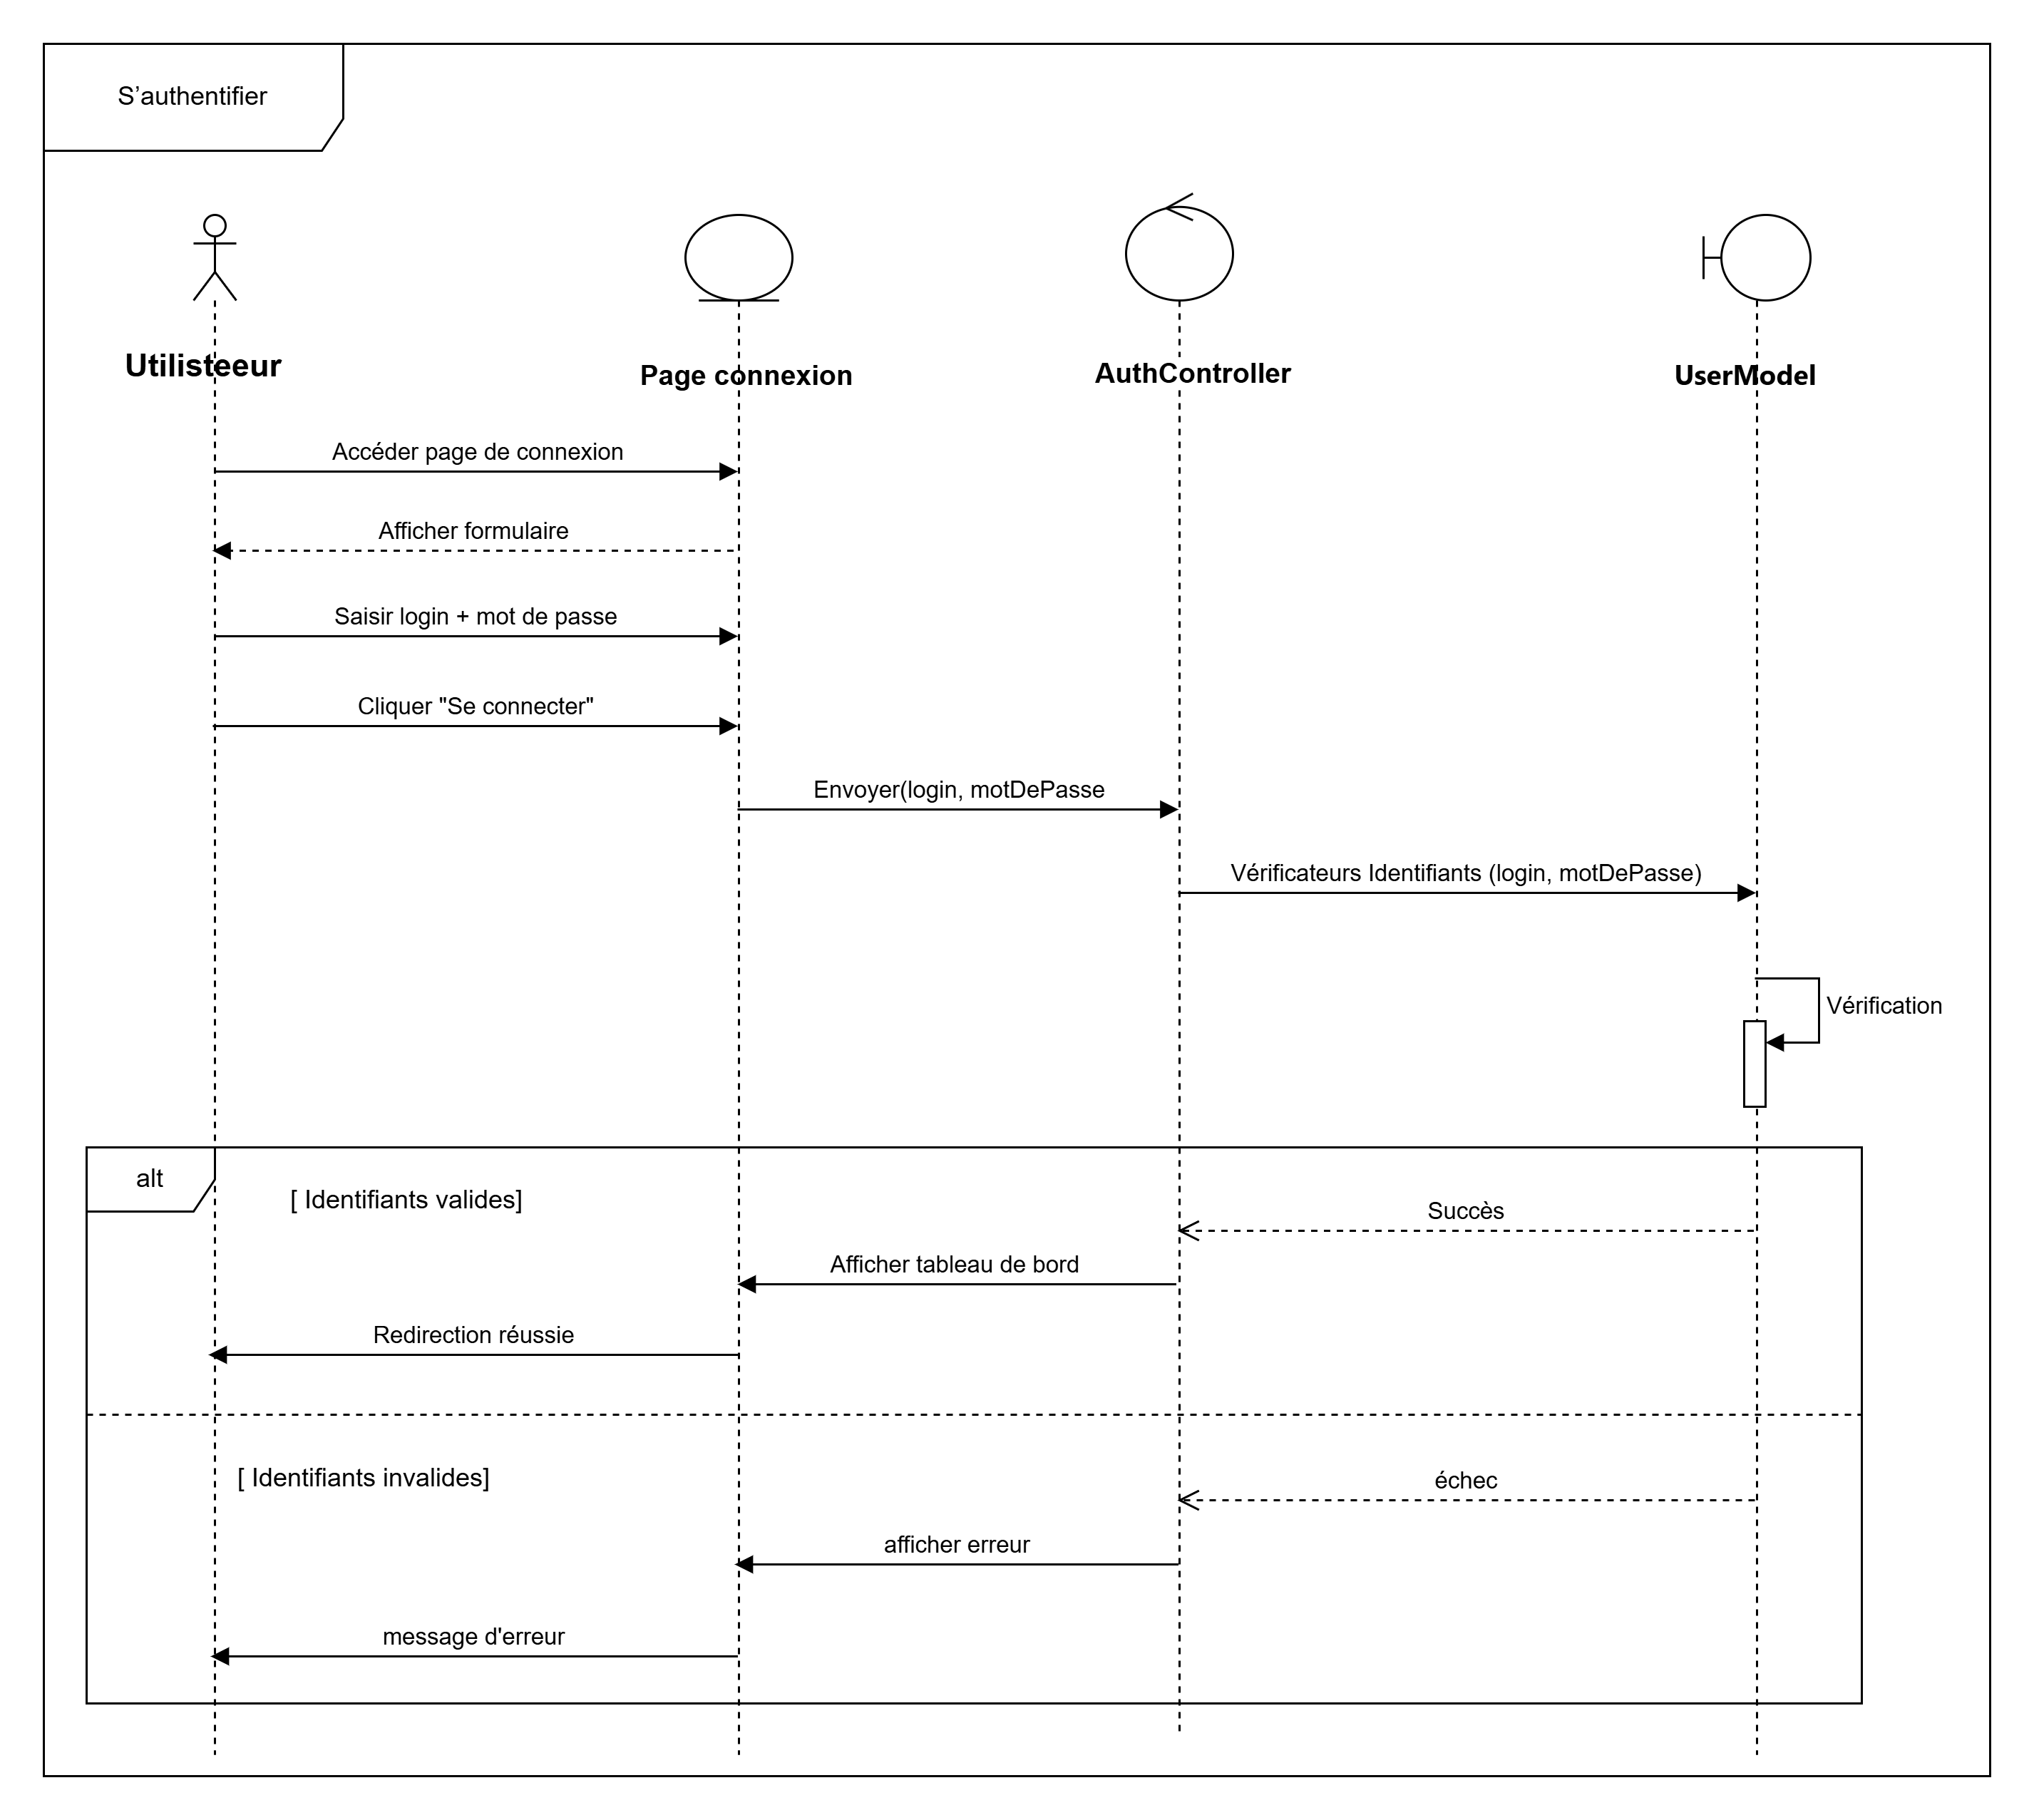
\includegraphics[width=0.9\textwidth]{projet/images/img sequence s1/auth.drawio.png}
    \caption{Diagramme de séquence du cas d'utilisation « S'authentifier »}
    \label{fig:interface6}
\end{figure}




Ce diagramme illustre les interactions entre l'utilisateur et le système lors de la réinitialisation du mot de passe, depuis la soumission de la demande jusqu'à la génération et l'envoi du nouveau mot de passe par e-mail.

\subsubsection*{Diagramme de séquence du cas d'utilisation « S'inscrire »}

Ce diagramme présente le processus d'inscription d'un nouveau Responsable RH sur la plateforme. Il saisit ses informations, le système vérifie leur validité, crée le compte et le redirige vers son tableau de bord.

\begin{figure}[H]
    \centering
    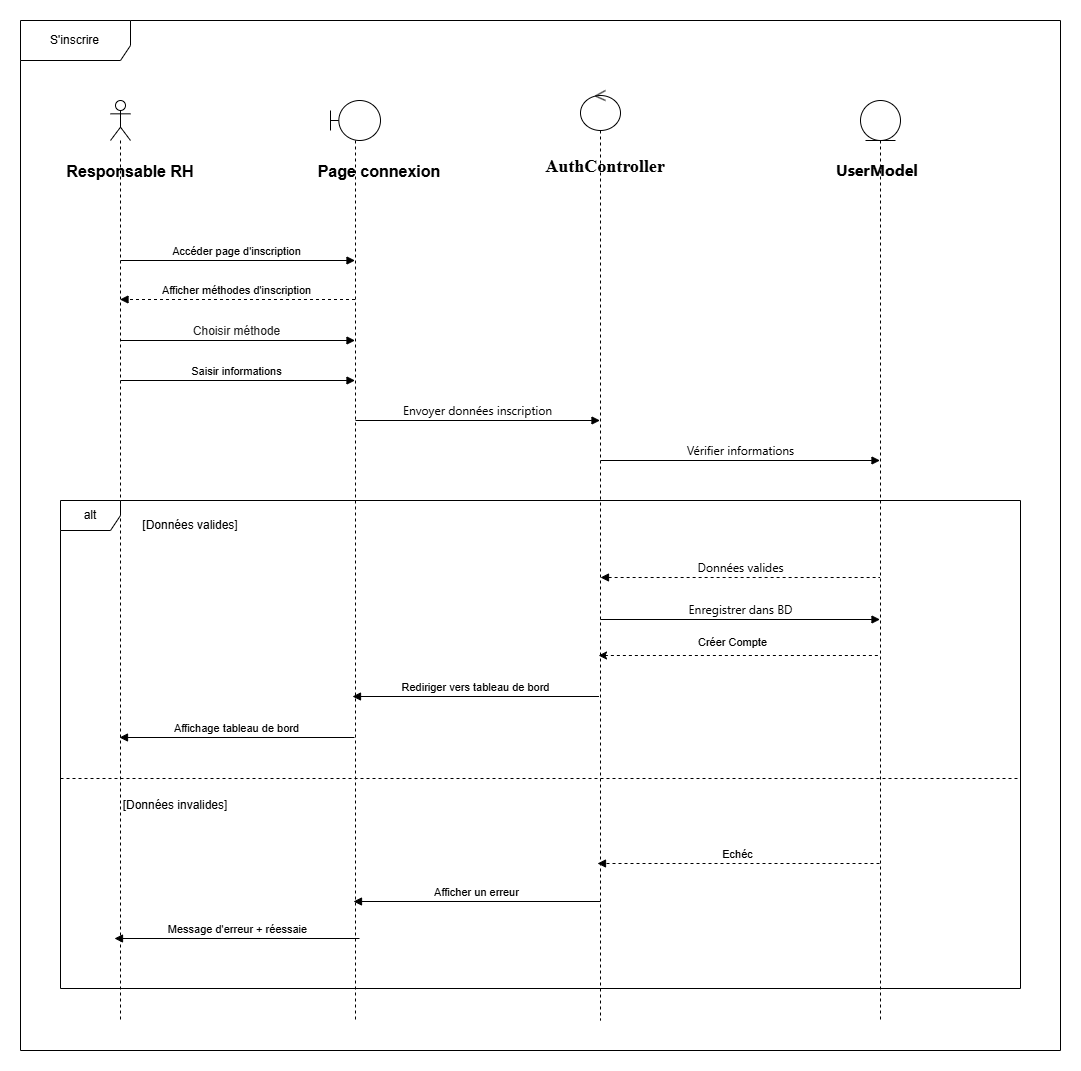
\includegraphics[width=0.9\textwidth]{projet/images/img sequence s1/sinscrire.drawio.png}
    \caption{Diagramme de séquence du cas d'utilisation « S'inscrire »}
\end{figure}


\subsubsection*{Diagramme de séquence du cas d'utilisation « Créer compte employé »}

Ce diagramme démontre la création d'un compte par le Responsable RH. Il entre les données de l'employé, puis le système valide ces informations et enregistre le nouvel employé.

\begin{figure}[H]
    \centering
    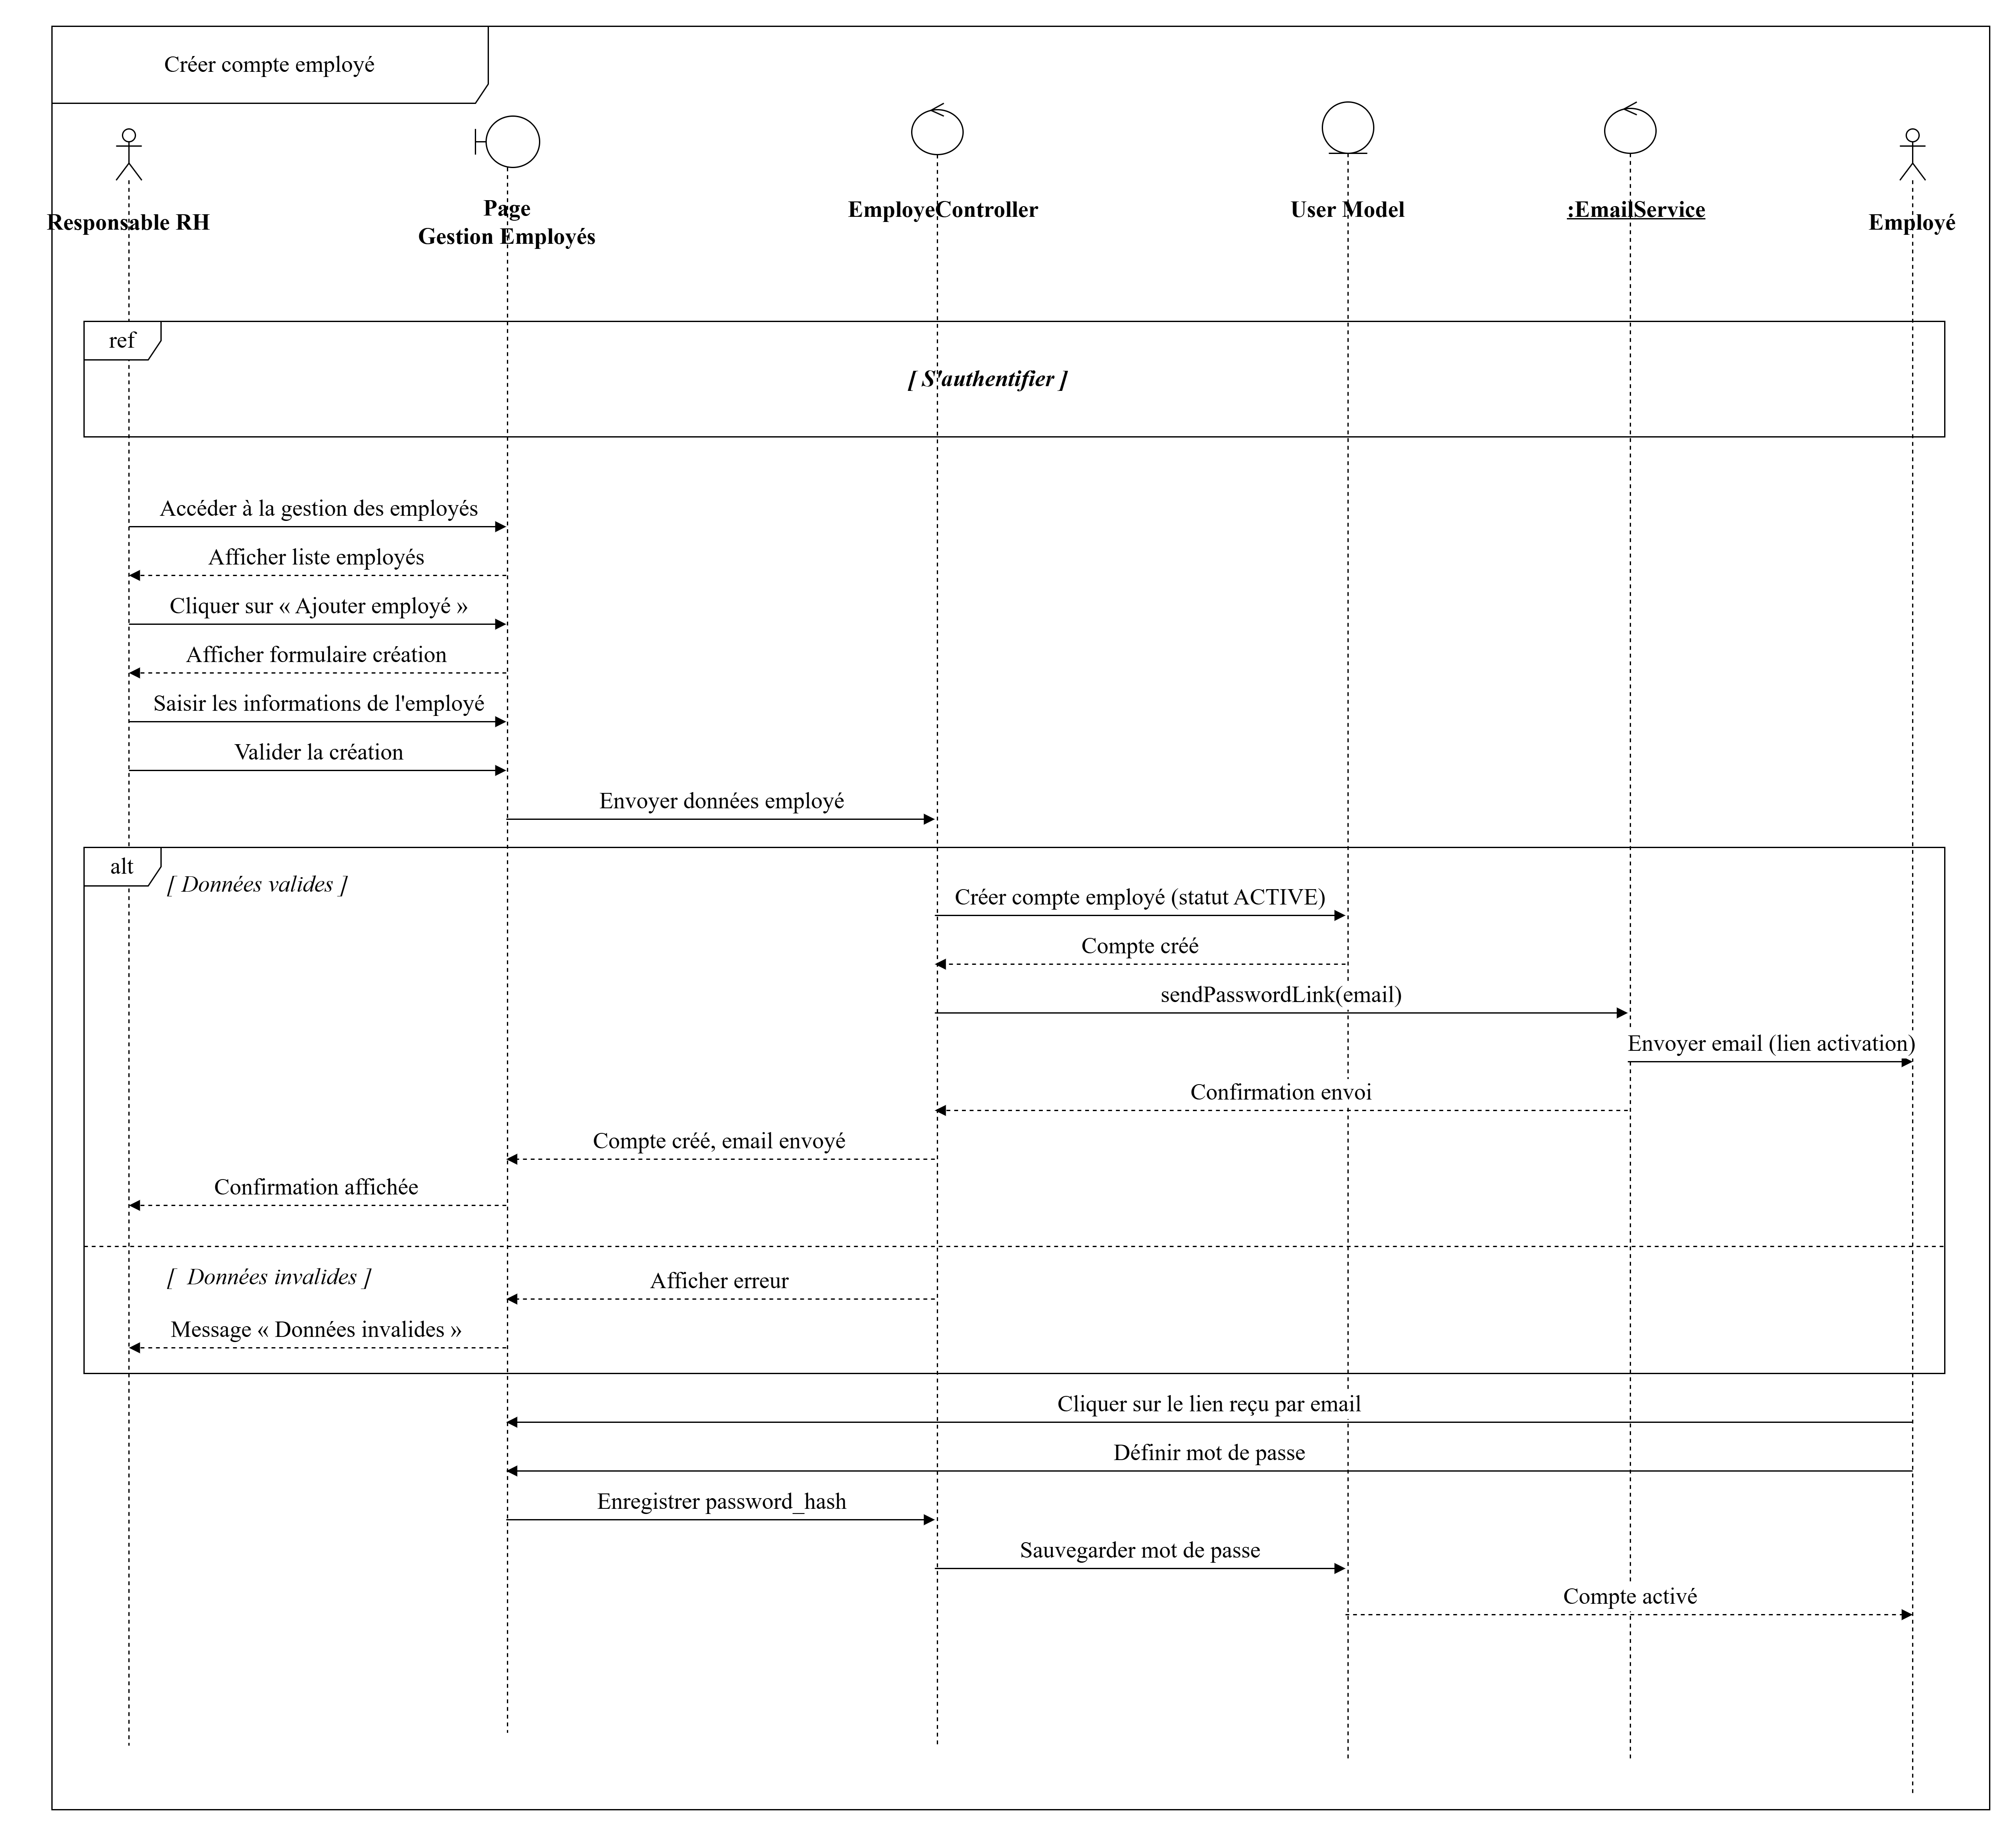
\includegraphics[width=0.9\textwidth]{projet/images/img sequence s1/creer_compte_employe.png}
    \caption{Diagramme de séquence du cas d'utilisation « Créer compte employé »}
\end{figure}


\subsubsection*{Diagramme de séquence du cas d'utilisation « Supprimer compte employé »}

Ce diagramme présente la suppression d'un compte employé par le Responsable RH. Après sélection du compte, le système demande une confirmation avant de procéder à la suppression définitive des données associées.

\begin{figure}[H]
    \centering
    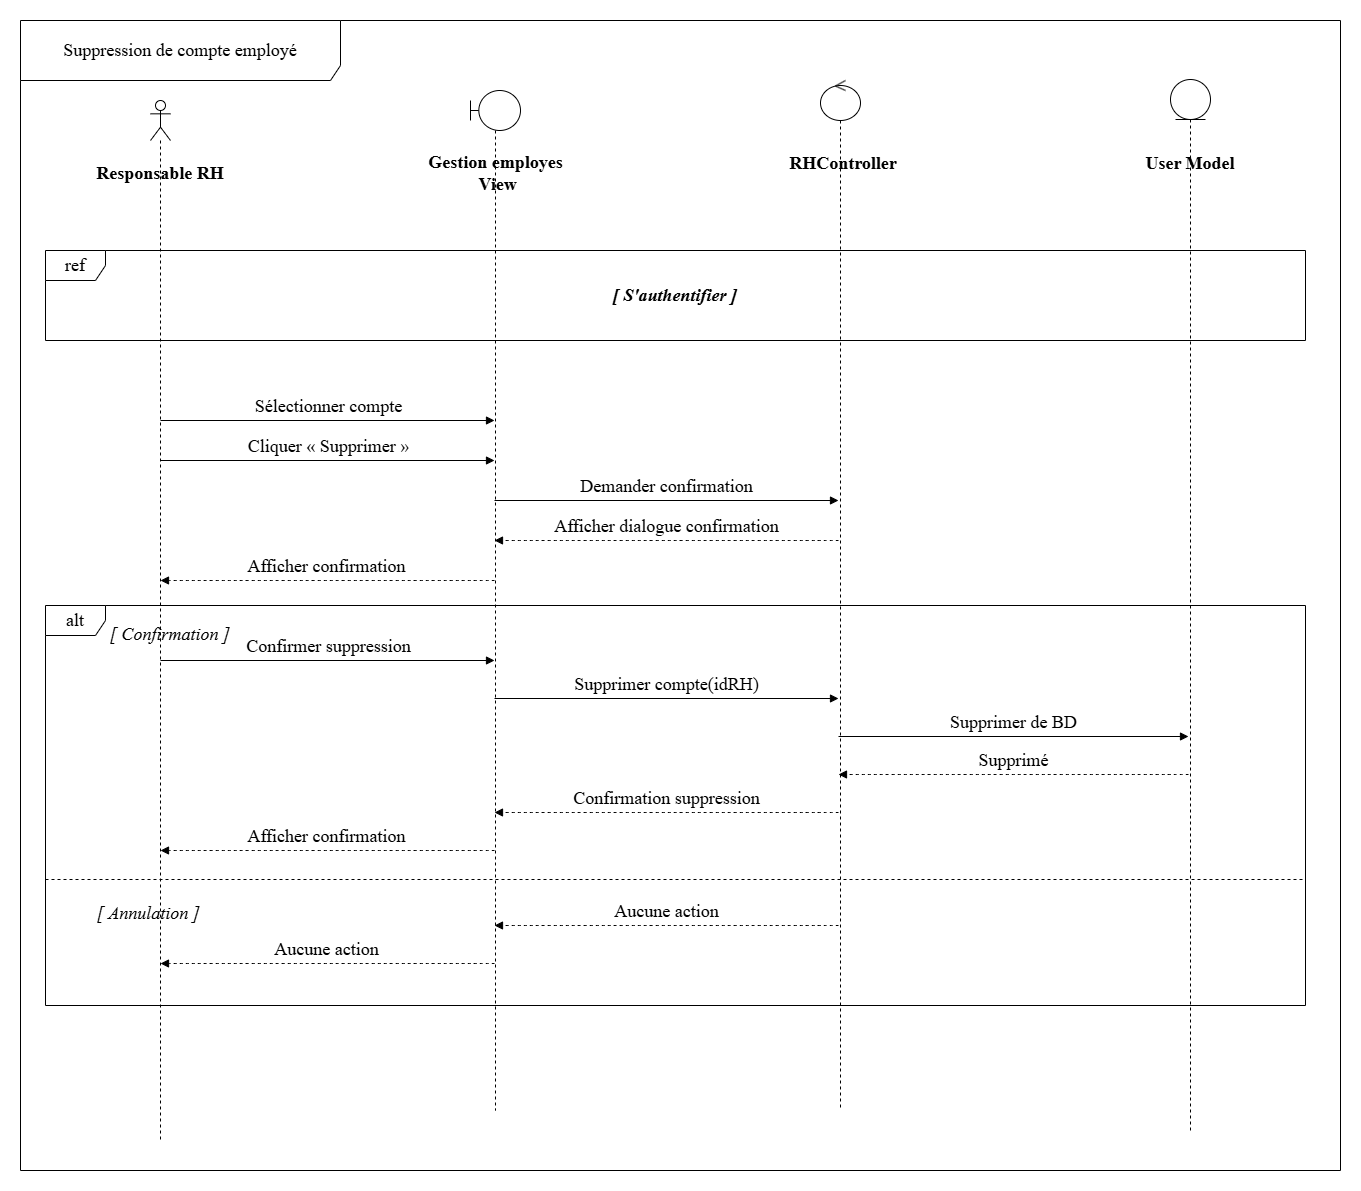
\includegraphics[width=0.9\textwidth]{projet/images/img sequence s1/sup.drawio.png}
    \caption{Diagramme de séquence du cas d'utilisation « Supprimer compte employé »}
\end{figure}


\subsubsection*{Diagramme de séquence du cas d'utilisation « Modifier compte Responsable RH »}

Ce diagramme décrit la modification des informations d'un compte Responsable RH par l'Administrateur. Il sélectionne le compte, met à jour les champs souhaités et le système enregistre les modifications après validation.

\begin{figure}[H]
    \centering
    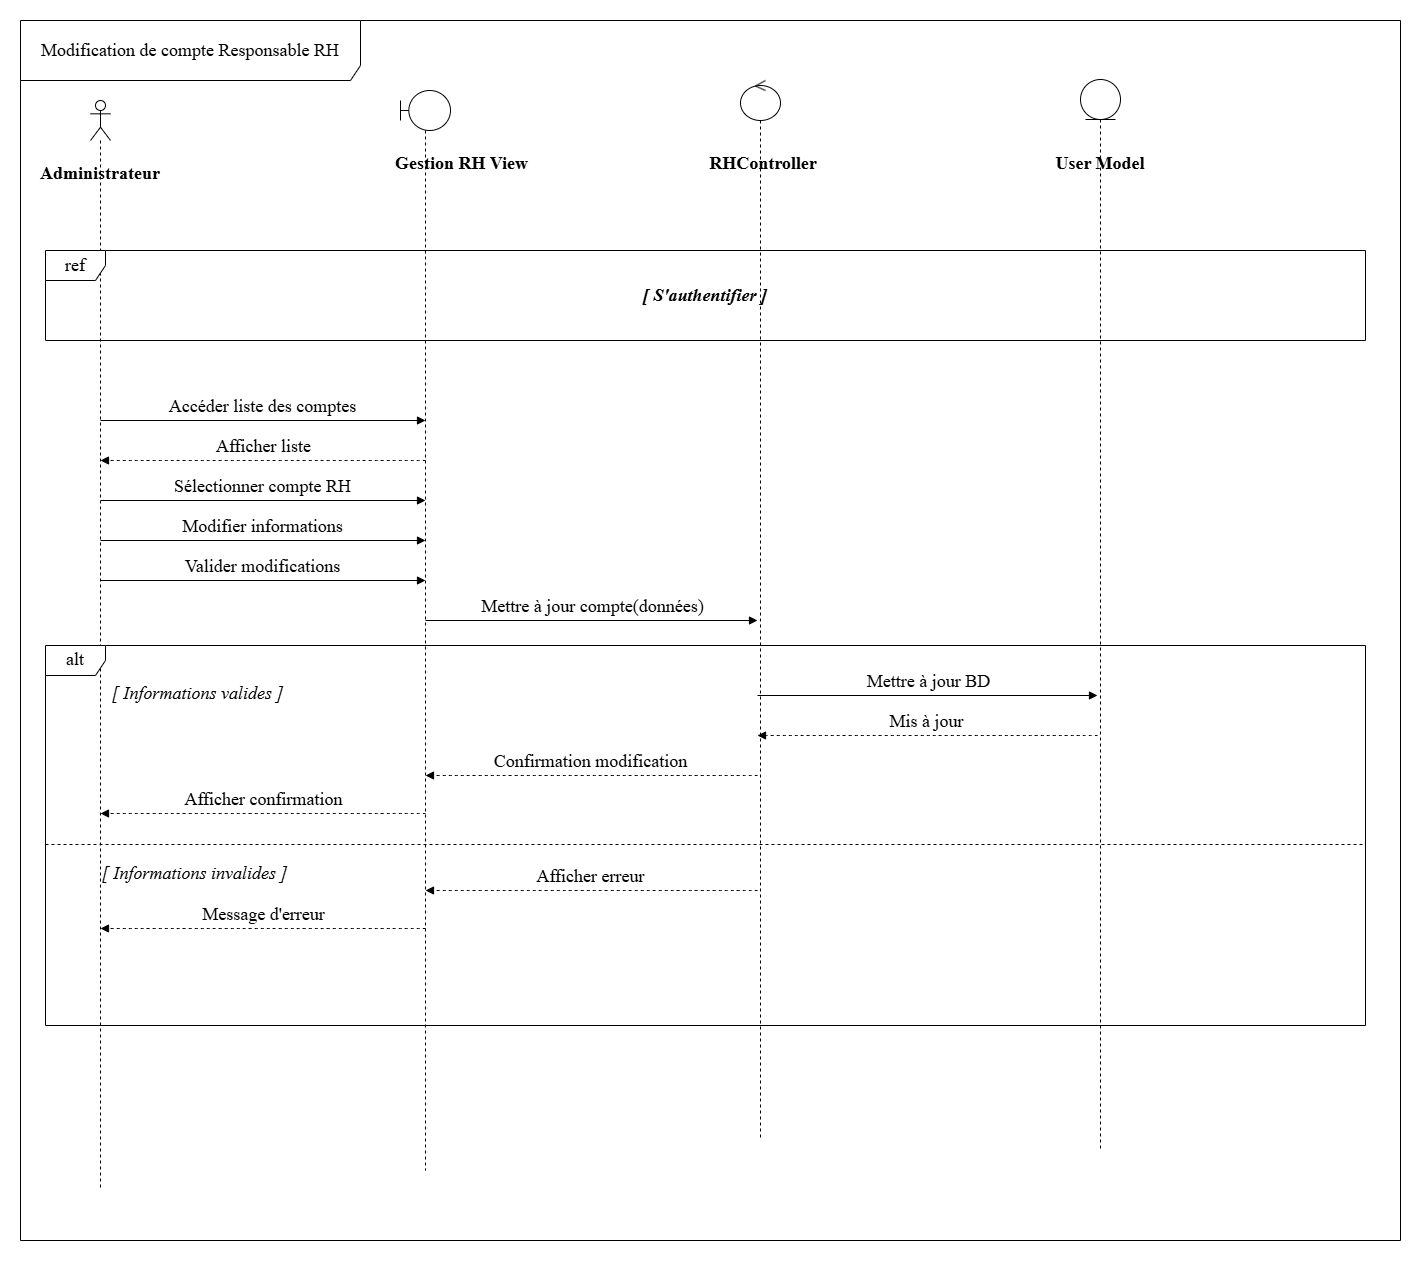
\includegraphics[width=0.9\textwidth]{projet/images/img sequence s1/modifier_compte_rhg.drawio.png}
    \caption{Diagramme de séquence du cas d'utilisation « Modifier compte Responsable RH »}
\end{figure}


\subsubsection{Diagramme de classe du sprint 1}

Ce diagramme de classe illustre la structure du module de gestion des accès et des comptes utilisateurs du système, en affichant les différentes classes, leurs attributs et les relations entre Administrateur, Responsable RH et Employé.

\begin{figure}[H]
    \centering
    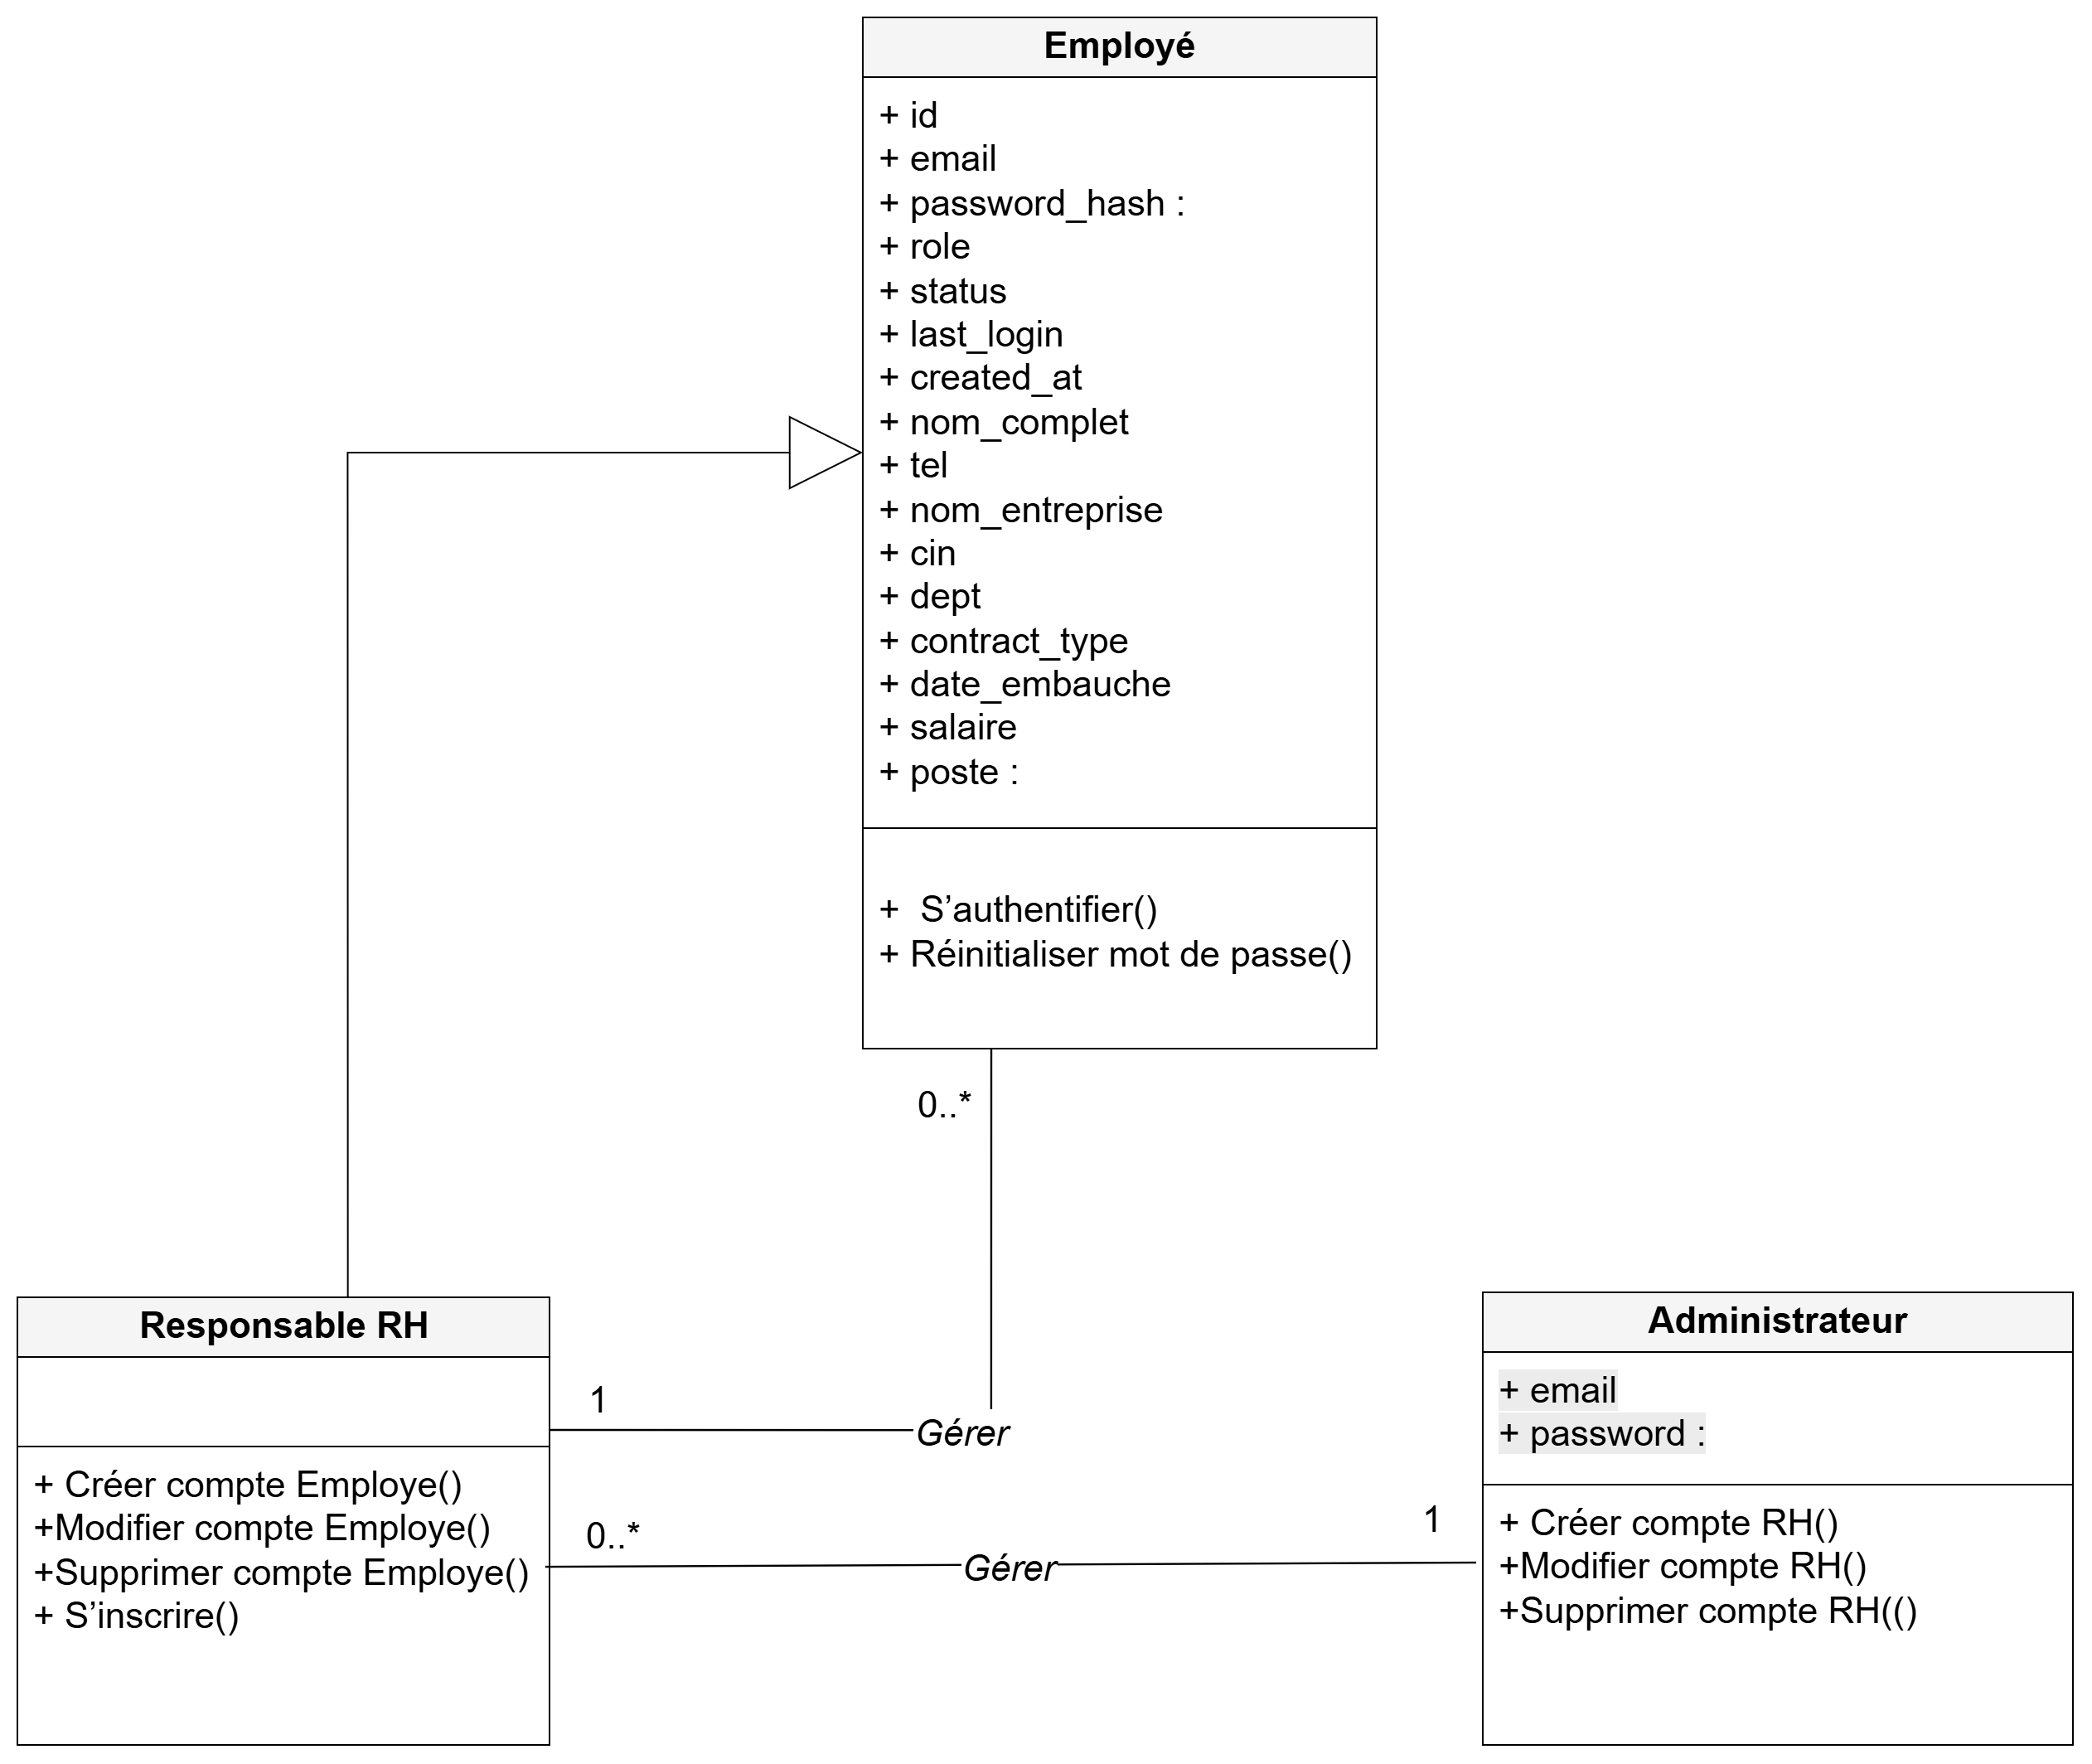
\includegraphics[width=0.9\textwidth]{projet/images/classe finale/diagramme_de_classe_s1.png}
    \caption{Diagramme de classe du sprint 1}
    \label{fig:classe1}
\end{figure}


%============================================================
\subsection{Interfaces réalisées pour le sprint 1}
%============================================================

\subsubsection*{Interface d'authentification}

Cette interface présente la page d'authentification. En effet, chaque utilisateur doit saisir son login et son mot de passe.

\begin{figure}[H]
    \centering
    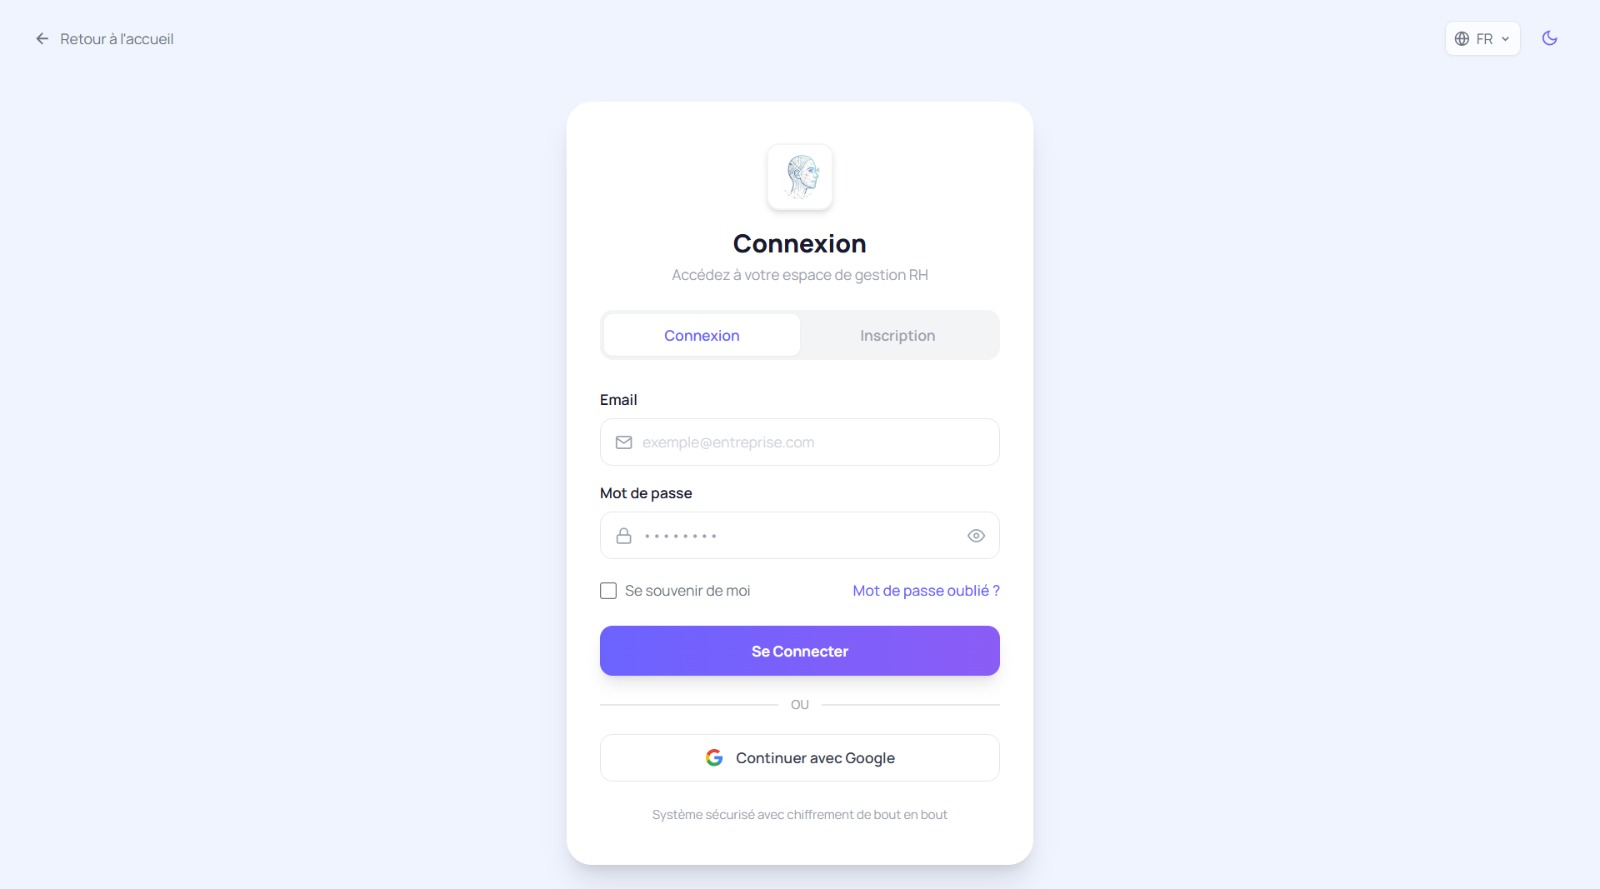
\includegraphics[width=0.9\textwidth]{projet/images/interface/s1/connexion.jpeg}
    \caption{Interface d'authentification}
    \label{fig:interface1}
\end{figure}


\subsubsection*{Interface d'inscription}

Cette interface présente la page d'inscription. En effet, le Responsable RH doit saisir les informations pour créer un nouveau compte.

\begin{figure}[H]
    \centering
    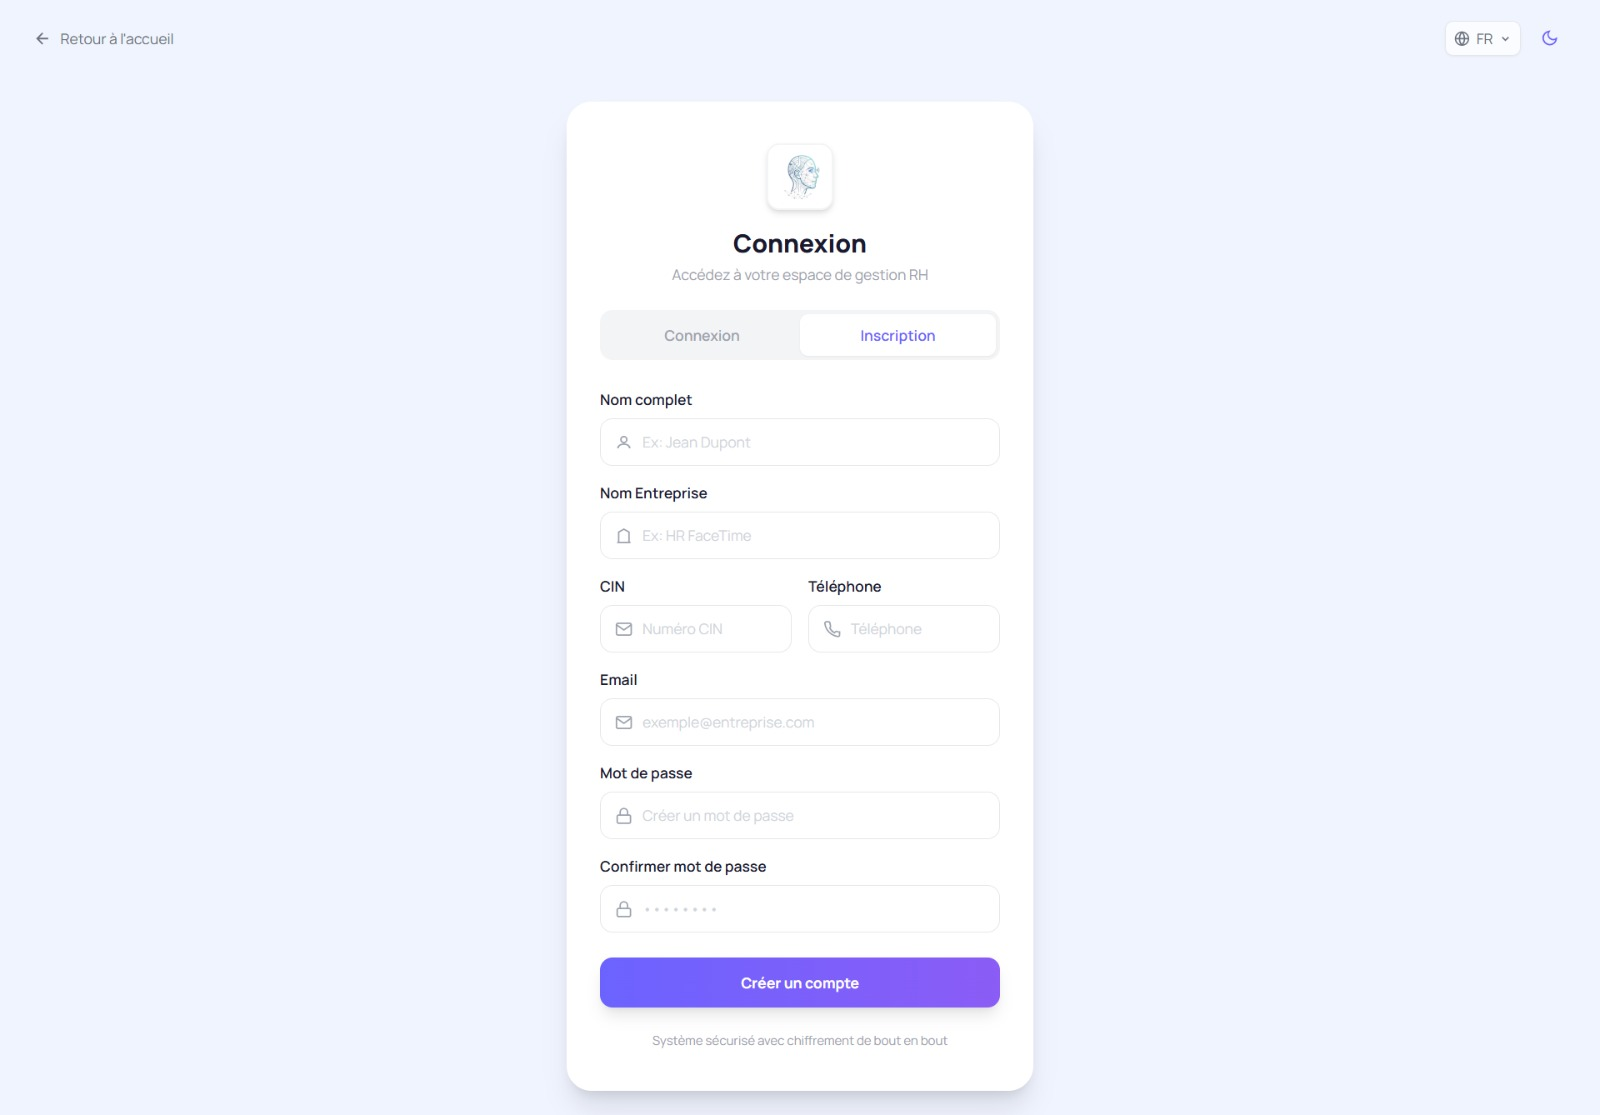
\includegraphics[width=0.9\textwidth]{projet/images/interface/s1/ins.jpeg}
    \caption{Interface d'inscription}
    \label{fig:interface2}
\end{figure}





\subsubsection*{Interface Gérer les comptes employés}

Cette interface permet au Responsable RH de gérer les comptes des employés (création, modification, suppression).

\begin{figure}[H]
    \centering
    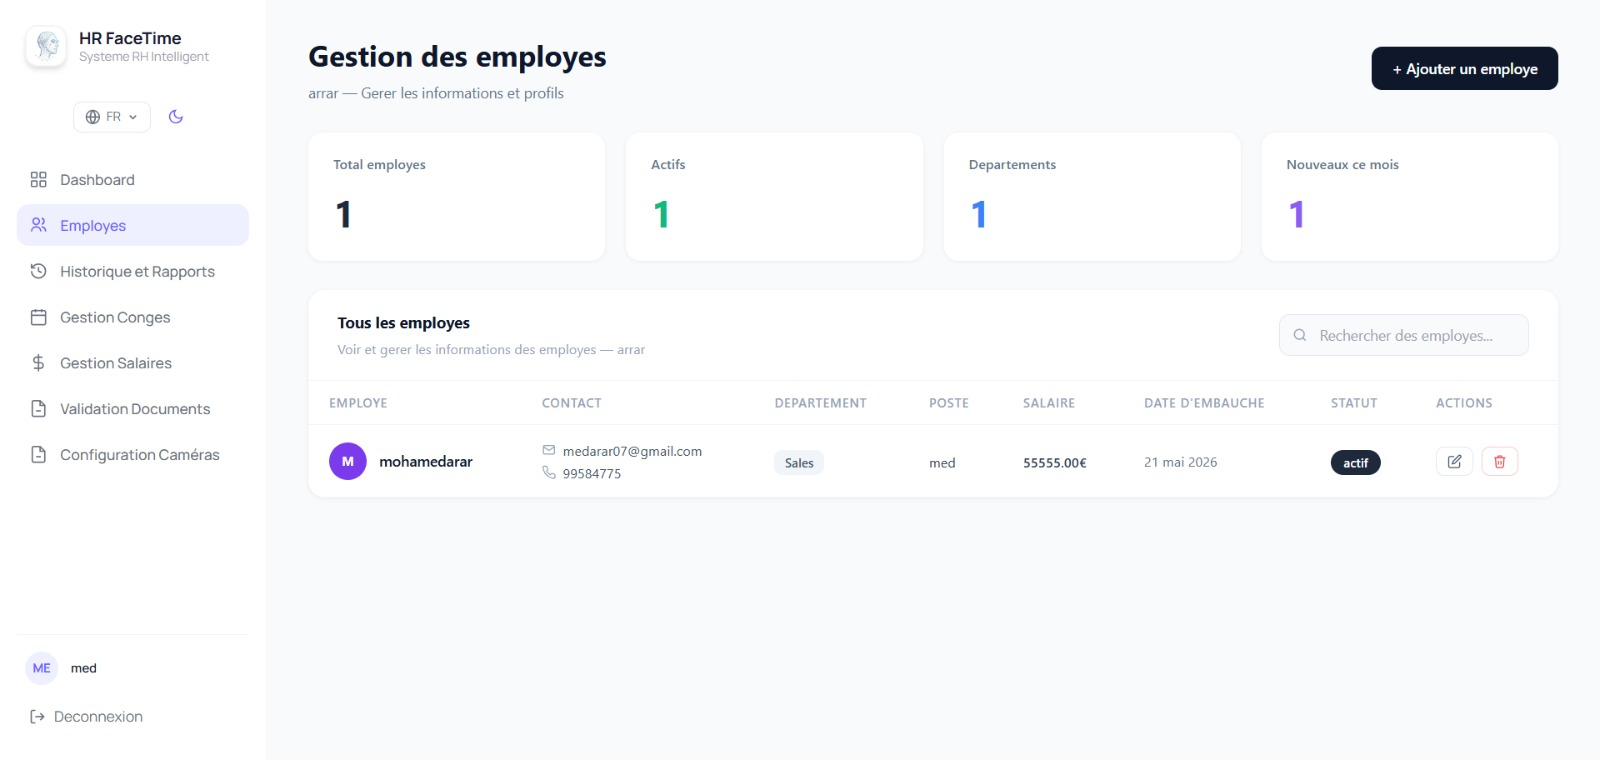
\includegraphics[width=0.9\textwidth]{projet/images/interface/s1/gestion employe.jpeg}
    \caption{Interface Gérer les comptes employés}
    \label{fig:interface4}
\end{figure}


\subsubsection*{Interface Gérer les comptes Responsables RH}

Cette interface permet à l'Administrateur de gérer les comptes des responsables RH (création, modification, suppression).

\begin{figure}[H]
    \centering
    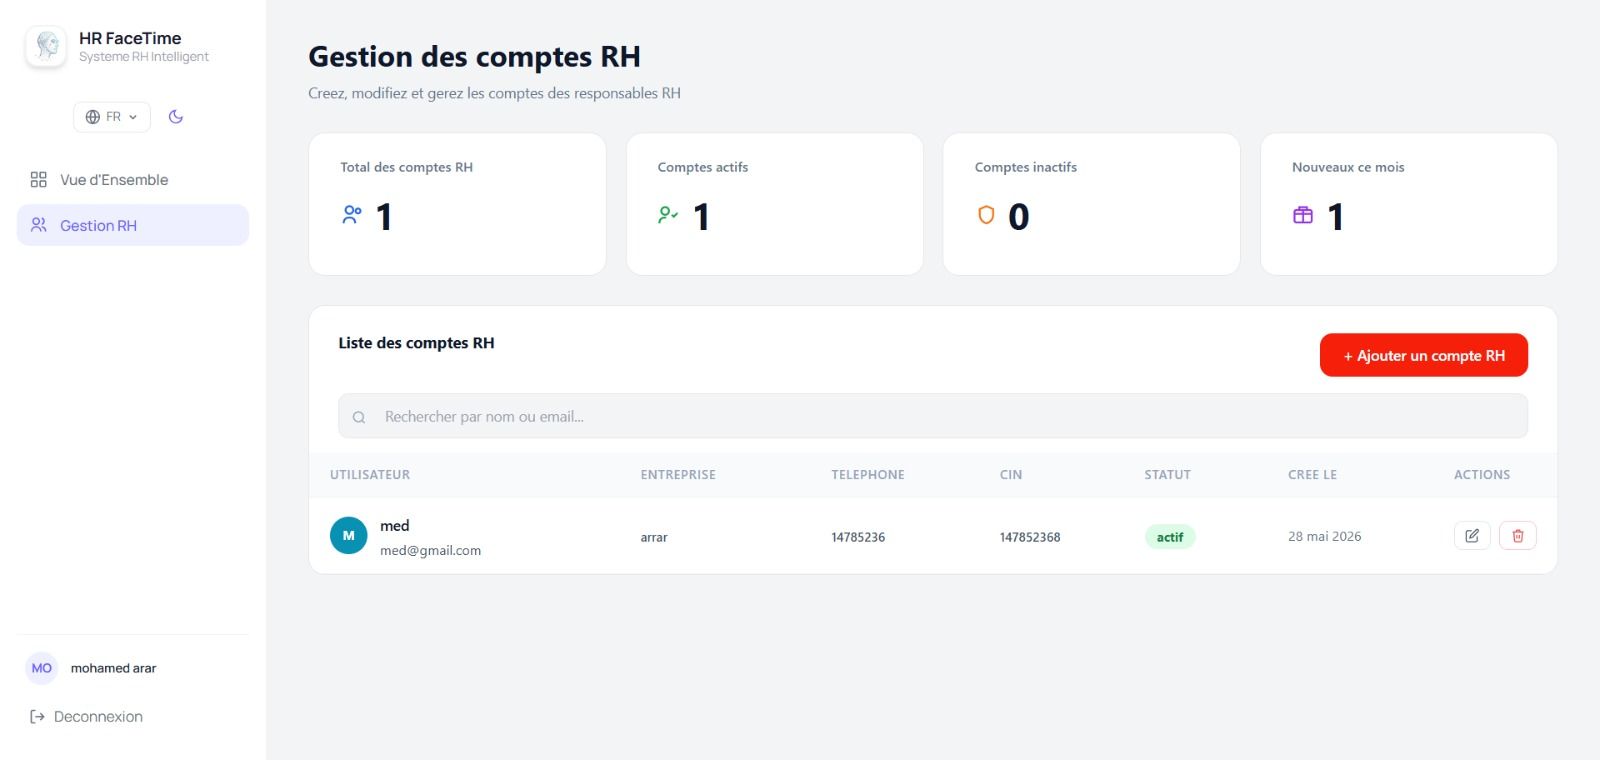
\includegraphics[width=0.9\textwidth]{projet/images/interface/s1/gestion rh.jpeg}
    \caption{Interface Gérer les comptes Responsables RH}
    \label{fig:interface5}
\end{figure}


%============================================================
\section{Sprint 2 : Pointage Intelligent et Suivi de Présence}
%============================================================

Ce sprint consiste à concevoir le module de pointage intelligent utilisant la reconnaissance faciale, afin d'identifier automatiquement les employés et de suivre leur présence dans l'entreprise.

\subsection{Objectif du sprint 2}

L'objectif de ce sprint est d'implémenter le pointage automatique par reconnaissance faciale, de connecter les caméras et de permettre le suivi des présences, absences et informations des employés.

\subsection{Durée du sprint 2}

\begin{itemize}
    \item \textbf{Date de début du sprint} : 12/03/2026
    \item \textbf{Date de fin du sprint} : 06/04/2026
\end{itemize}

\subsection{Backlog du sprint 2}
Ce tableau liste les cinq user stories du sprint 2, portant sur la connexion des caméras, l'enregistrement du visage, la modification des informations personnelles, la consultation des absences et le pointage facial. Les priorités élevées reflètent la complexité technique liée à l'intelligence artificielle et à la reconnaissance faciale.

\begin{longtable}{|>{\centering\arraybackslash}m{0.5cm}|
    >{\centering\arraybackslash}m{3cm}|
    >{\centering\arraybackslash}m{2.5cm}|
    >{\centering\arraybackslash}m{3cm}|
    >{\centering\arraybackslash}m{3cm}|
    >{\centering\arraybackslash}m{0.7cm}|
    >{\centering\arraybackslash}m{0.9cm}|}
\hline
\textbf{ID} & \textbf{User Story} & \textbf{En tant que} & \textbf{Je veux} & \textbf{Afin de} & \textbf{P} & \textbf{C} \\
\hline
\endfirsthead
\hline
\textbf{ID} & \textbf{User Story} & \textbf{En tant que} & \textbf{Je veux} & \textbf{Afin de} & \textbf{P} & \textbf{C} \\
\hline
\endhead
10 & Connecter la plateforme aux caméras & Responsable RH & configurer et connecter les caméras    & activer le pointage automatique     & 5 & 5 \\ \hline
22 & Enregistrer le visage               & Employé        & enregistrer mon visage                 & permettre le pointage automatique   & 5 & 5 \\ \hline
23 & Modifier infos personnelles         & Employé        & modifier mes informations personnelles & maintenir mes données à jour        & 3 & 2 \\ \hline
24 & Consulter ses absences              & Employé        & consulter mes absences                 & suivre ma présence                  & 3 & 2 \\ \hline
30 & Pointage faciale               & Employé        & pointer ma présence par reconnaissance faciale & automatiser le pointage et éviter les oublis de pointage & 5 & 5 \\ \hline
\caption{Backlog Sprint 2 — Pointage Intelligent \& Présence}
\end{longtable}


%============================================================
\subsection{Spécification fonctionnelle détaillée}
%============================================================

\subsubsection*{Diagramme de cas d'utilisation du sprint 2}
Ce diagramme présente les interactions entre le Responsable RH et l'Employé avec les fonctionnalités du sprint 2, notamment la configuration des caméras et les différentes actions liées au pointage intelligent par reconnaissance faciale.

\begin{figure}[H]
    \centering
    
\includegraphics[width=0.9\textwidth]{projet/images/usecase/sprint2/sprint2.drawio.png}
    \caption{Diagramme de Cas d'utilisation du Sprint 2}
    \label{fig:usecase4}
\end{figure}


\subsubsection*{Description textuelle : cas d'utilisation « Connecter la plateforme aux caméras »}
Ce tableau décrit les étapes de configuration et de connexion des caméras par le Responsable RH, depuis l'accès au module jusqu'à l'activation du pointage automatique, ainsi que le scénario d'exception en cas d'échec de connexion.

\begin{longtable}{|p{5cm}|p{11cm}|}
\hline
\textbf{Nom du cas d'utilisation} & \textbf{Connecter la plateforme aux caméras} \\ \hline
\textbf{Acteurs}                  & Responsable RH \\ \hline
\textbf{Objectif}                 & Configurer et connecter les caméras \\ \hline
\textbf{Préconditions}            & Le Responsable RH doit être authentifié \\ \hline
\textbf{Scénario nominal} &
1. Le Responsable RH accède aux « Configuration Caméras ». \newline
2. Il choisit l'option « Détecter les caméras ». \newline
3. Il définit la caméra d'entrée et la caméra de sortie. \newline
4. Il valide la configuration. \newline
5. Le système connecte les caméras et active le pointage automatique. \\ \hline
\textbf{Scénario d'exception} &
5.1 Si la connexion échoue, le système demande de réessayer. \\ \hline
\textbf{Post-condition} & Les caméras sont connectées et le pointage automatique est activé. \\ \hline
\caption{Description textuelle du cas d'utilisation « Connecter la plateforme aux caméras »}
\end{longtable}


\subsubsection*{Description textuelle : cas d'utilisation « Enregistrer le visage »}
Ce tableau présente le processus d'enregistrement biométrique du visage d'un employé lors de sa première connexion, incluant la capture par caméra et le stockage des données faciales dans le système pour permettre le pointage automatique.

\begin{longtable}{|p{5cm}|p{11cm}|}
\hline
\textbf{Nom du cas d'utilisation} & \textbf{Enregistrer le visage} \\ \hline
\textbf{Acteurs}                  & Employé \\ \hline
\textbf{Objectif}                 & Enregistrer le visage pour le pointage automatique \\ \hline
\textbf{Préconditions}            & L'employé doit être authentifié \\ \hline
\textbf{Scénario nominal} &
1. L'employé saisit ses informations de connexion. \newline
2. Le système vérifie les informations. \newline
3. Lors de la première connexion, le système demande l'enregistrement du visage. \newline
4. L'employé autorise l'accès à la caméra. \newline
5. La caméra capture le visage. \newline
6. Le système enregistre les données. \newline
7. L'employé accède à son espace personnel. \\ \hline
\textbf{Scénario d'exception} &
3.1 Si la capture échoue, le système demande de recommencer. \\ \hline
\textbf{Post-condition} & Le visage est enregistré pour le pointage automatique. \\ \hline
\caption{Description textuelle du cas d'utilisation « Enregistrer le visage »}
\end{longtable}


\subsubsection*{Description textuelle : cas d'utilisation « Modifier infos personnelles »}
Ce tableau décrit les étapes permettant à l'employé de consulter et de mettre à jour ses informations personnelles depuis son profil, ainsi que le scénario d'exception déclenché en cas de saisie de données invalides.

\begin{longtable}{|p{5cm}|p{11cm}|}
\hline
\textbf{Nom du cas d'utilisation} & \textbf{Modifier infos personnelles} \\ \hline
\textbf{Acteurs}                  & Employé \\ \hline
\textbf{Objectif}                 & Modifier ses informations personnelles \\ \hline
\textbf{Préconditions}            & Employé authentifié \\ \hline
\textbf{Scénario nominal} &
1. L'employé accède à « Mon Profil ». \newline
2. Il visualise ses données personnelles (nom, email, poste, etc.). \newline
3. Il met à jour les champs souhaités. \newline
4. Il valide les modifications. \newline
5. Le système enregistre les changements. \\ \hline
\textbf{Scénario d'exception} &
3.1 Si les champs sont invalides, le système affiche « Modification impossible ». \\ \hline
\textbf{Post-condition} & Les informations personnelles sont consultées et/ou mises à jour. \\ \hline
\caption{Description textuelle du cas d'utilisation « Modifier infos personnelles »}
\end{longtable}


\subsubsection*{Description textuelle : cas d'utilisation « Consulter mes absences »}
Ce tableau présente le scénario de consultation par l'employé de son historique d'absences et de retards depuis son tableau de bord, avec le cas d'exception affiché en l'absence de données disponibles dans le système.

\begin{longtable}{|p{5cm}|p{11cm}|}
\hline
\textbf{Nom du cas d'utilisation} & \textbf{Consulter mes absences} \\ \hline
\textbf{Acteurs}                  & Employé \\ \hline
\textbf{Objectif}                 & Consulter ses absences et retards \\ \hline
\textbf{Préconditions}            & L'employé doit être authentifié \\ \hline
\textbf{Scénario nominal} &
1. L'employé accède à son tableau de bord. \newline
2. Il consulte la section « Mes Absences ». \newline
3. Le système affiche ses absences . \\ \hline
\textbf{Scénario d'exception} &
2.1 Si aucune donnée n'est disponible, le système affiche un message. \\ \hline
\textbf{Post-condition} & L'employé visualise ses informations de présence. \\ \hline
\caption{Description textuelle du cas d'utilisation « Consulter mes absences et retards »}
\end{longtable}


\subsubsection*{Description textuelle : cas d'utilisation « Pointage Facial »}
Ce tableau détaille le scénario nominal du pointage facial en mode télétravail, couvrant les opérations de check-in et check-out via reconnaissance faciale, ainsi que l'exception déclenchée en cas d'échec d'identification du visage par le système.

\begin{center}
\begin{longtable}{|p{5cm}|p{11cm}|}
\hline
\textbf{Nom du cas d'utilisation} & \textbf{Pointage Facial} \\ \hline

\textbf{Acteurs} & Employé \\ \hline

\textbf{Objectif} & Enregistrer sa présence à distance via la reconnaissance faciale. \\ \hline

\textbf{Préconditions} & L'employé doit être authentifié et son mode de travail doit être défini sur « Télétravail ». \\ \hline

\textbf{Scénario nominal} &

1. L'employé accède à l'interface de pointage. \newline
2. Il clique sur le bouton « Check In ». \newline
3. La caméra s'active et capture son visage. \newline
4. Le système effectue la reconnaissance faciale. \newline
5. Le système enregistre l'heure d'entrée et confirme le pointage. \newline
6. À la fin de sa journée de travail, l'employé clique sur le bouton « Check Out ». \newline
7. La caméra capture à nouveau son visage. \newline
8. Le système vérifie son identité et enregistre l'heure de sortie.
   \\ \hline

\textbf{Scénario d'exception} &
4.1 Si le visage n'est pas reconnu, le système affiche un message d'erreur et refuse le pointage.
\\ \hline

\textbf{Post-condition} & Les heures d'entrée et de sortie de l'employé sont enregistrées.
\\ \hline

\caption{Description textuelle du cas d'utilisation « Pointage Facial en Télétravail »}
\end{longtable}
\end{center}


%============================================================
\subsection{Conception}
%============================================================

Cette section présente les différents diagrammes UML réalisés afin de modéliser le fonctionnement du système, notamment les diagrammes de séquence et les diagrammes de classes, permettant de décrire les interactions entre les acteurs ainsi que la structure globale de l'application.

\subsubsection{Diagrammes de séquence du sprint 2}

\subsubsection*{Diagramme de séquence du cas d'utilisation « Connecter la plateforme aux caméras »}

Ce diagramme illustre la configuration et la connexion des caméras à la plateforme par le Responsable RH. Il saisit les paramètres de connexion, le système établit la liaison avec les caméras et active le module de pointage automatique par reconnaissance faciale.

\begin{figure}[H]
    \centering
    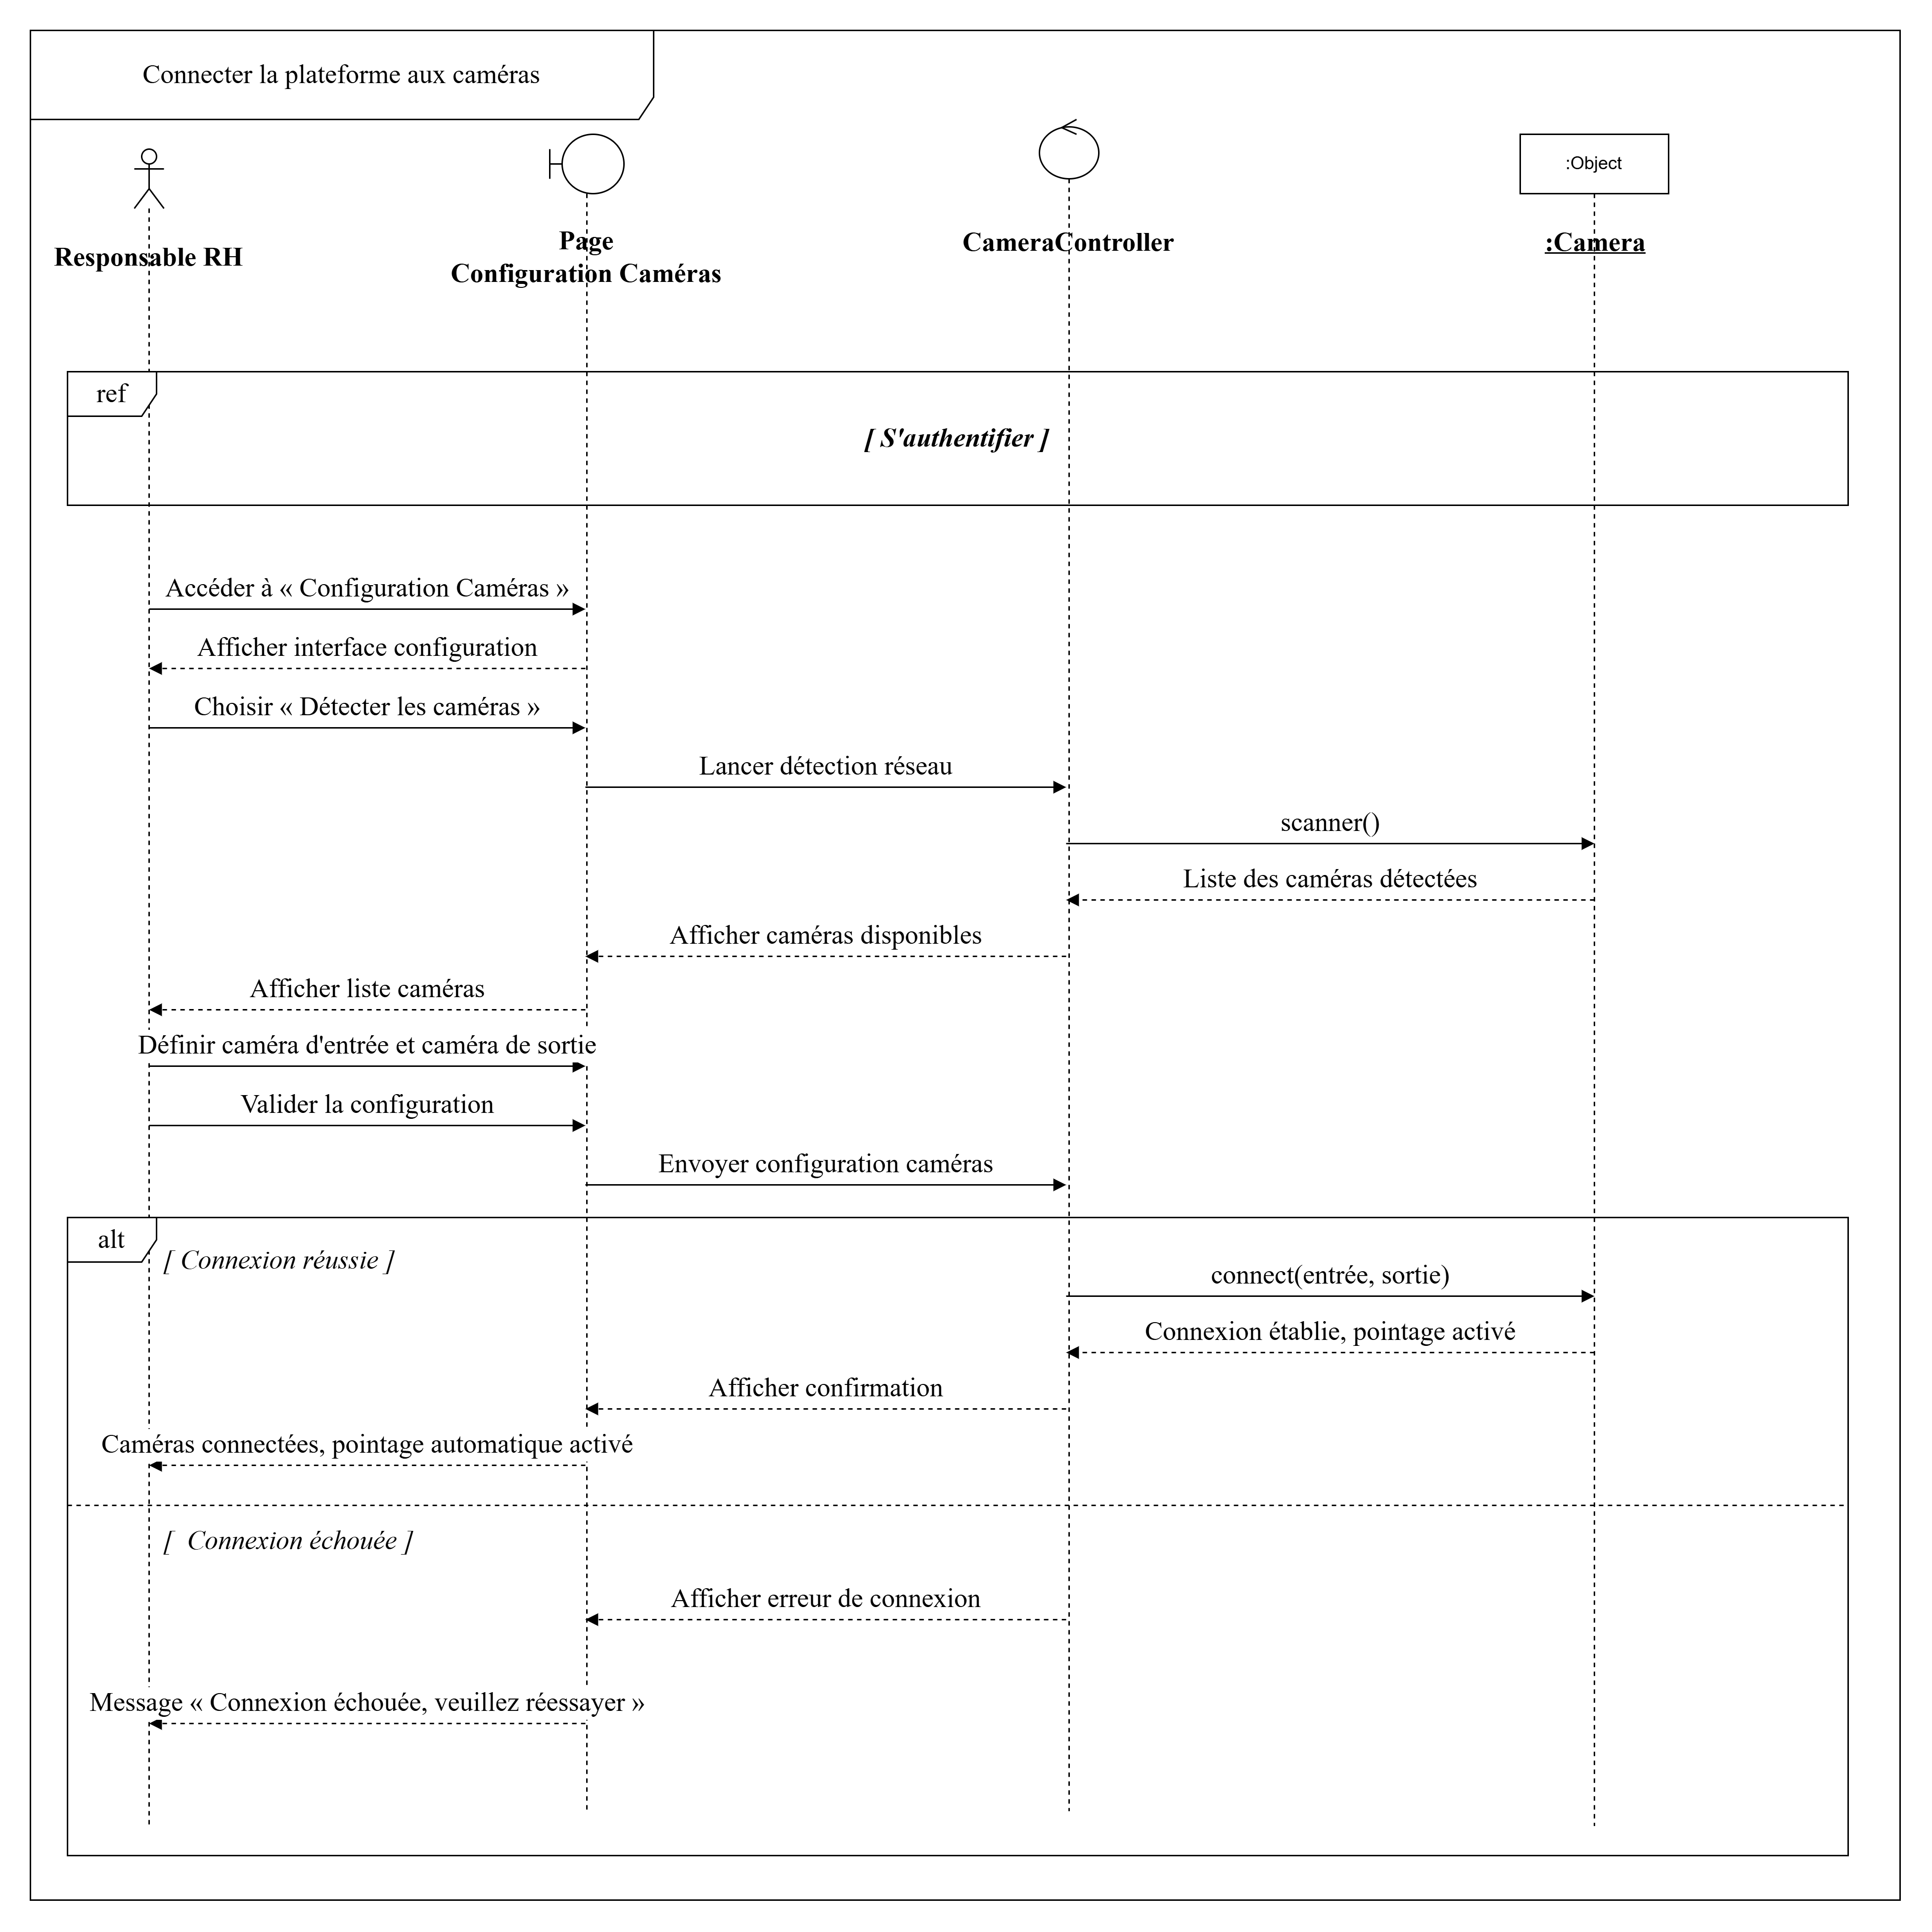
\includegraphics[width=0.85\textwidth]{projet/images/img diag sprint 2/connecter_cameras.png}
    \caption{Diagramme de séquence du cas d'utilisation « Connecter la plateforme aux caméras »}
\end{figure}


\subsubsection*{Diagramme de séquence du cas d'utilisation « Enregistrer le visage »}

Ce diagramme décrit le processus d'enregistrement du visage d'un employé pour le pointage automatique. La caméra capture le visage, le module d'intelligence artificielle traite et enregistre les données biométriques dans la base de données.

\begin{figure}[H]
    \centering
    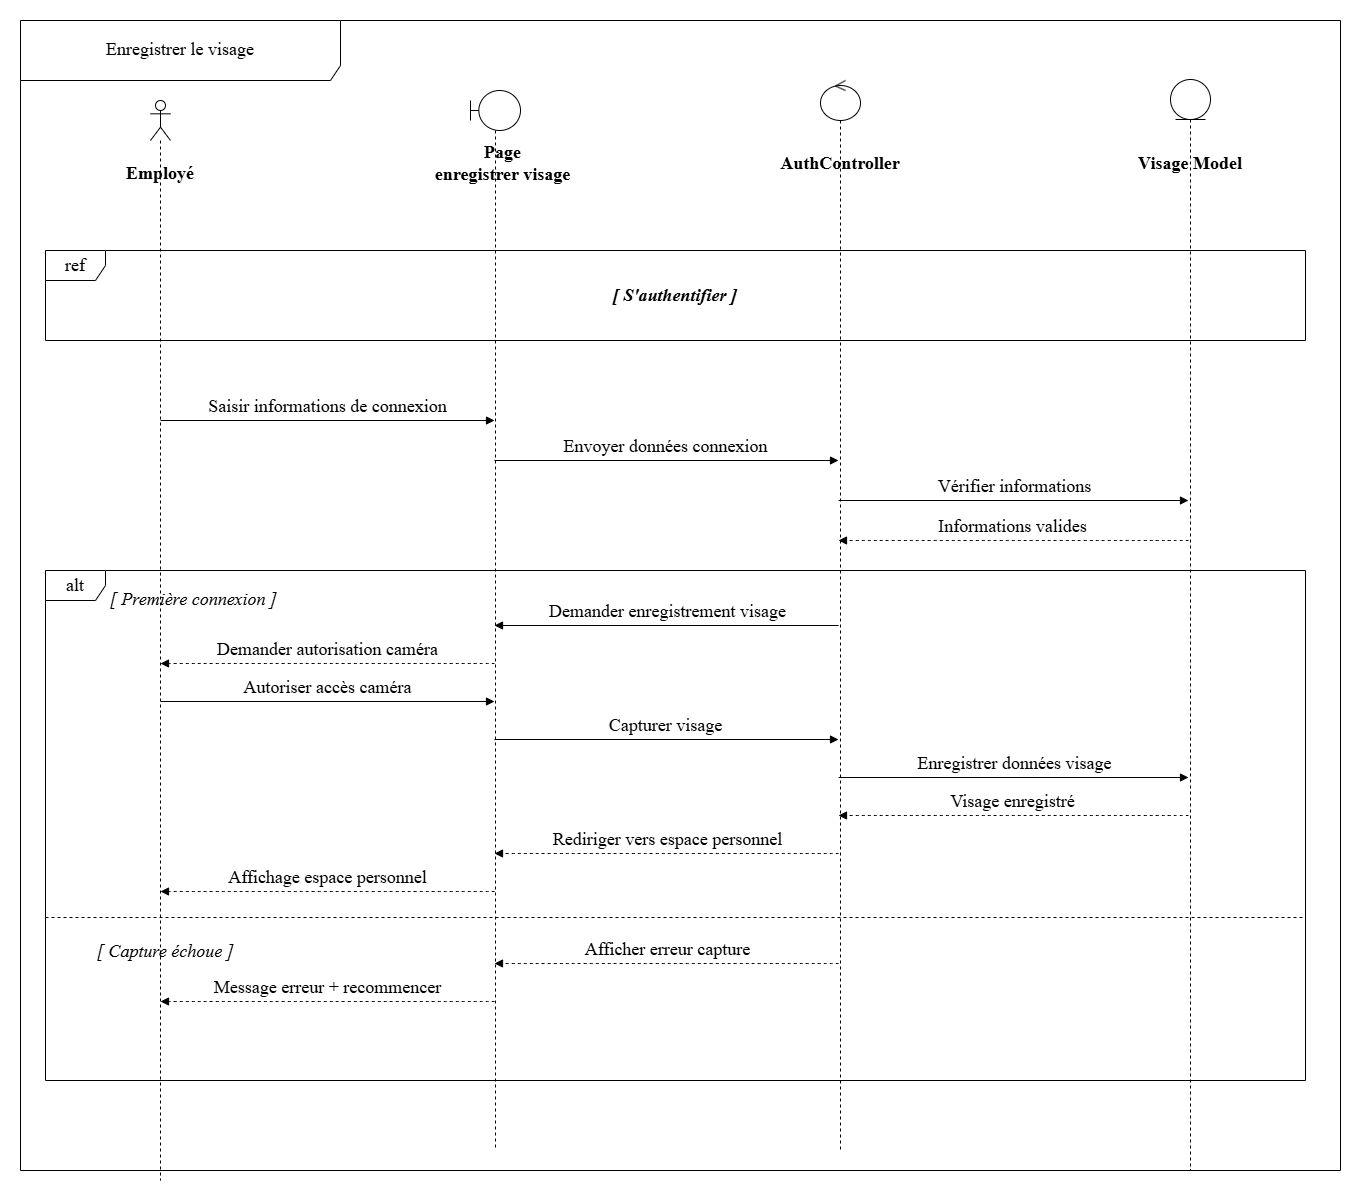
\includegraphics[width=0.85\textwidth]{projet/images/img diag sprint 2/enregister_visage.png}
    \caption{Diagramme de séquence du cas d'utilisation « Enregistrer le visage »}
\end{figure}


\subsubsection*{Diagramme de séquence du cas d'utilisation « Modifier infos personnelles »}

Ce diagramme illustre la mise à jour des informations personnelles par l'employé. Il modifie les champs souhaités, le système vérifie la validité des données saisies et enregistre les modifications avec une confirmation à l'utilisateur.

\begin{figure}[H]
    \centering
    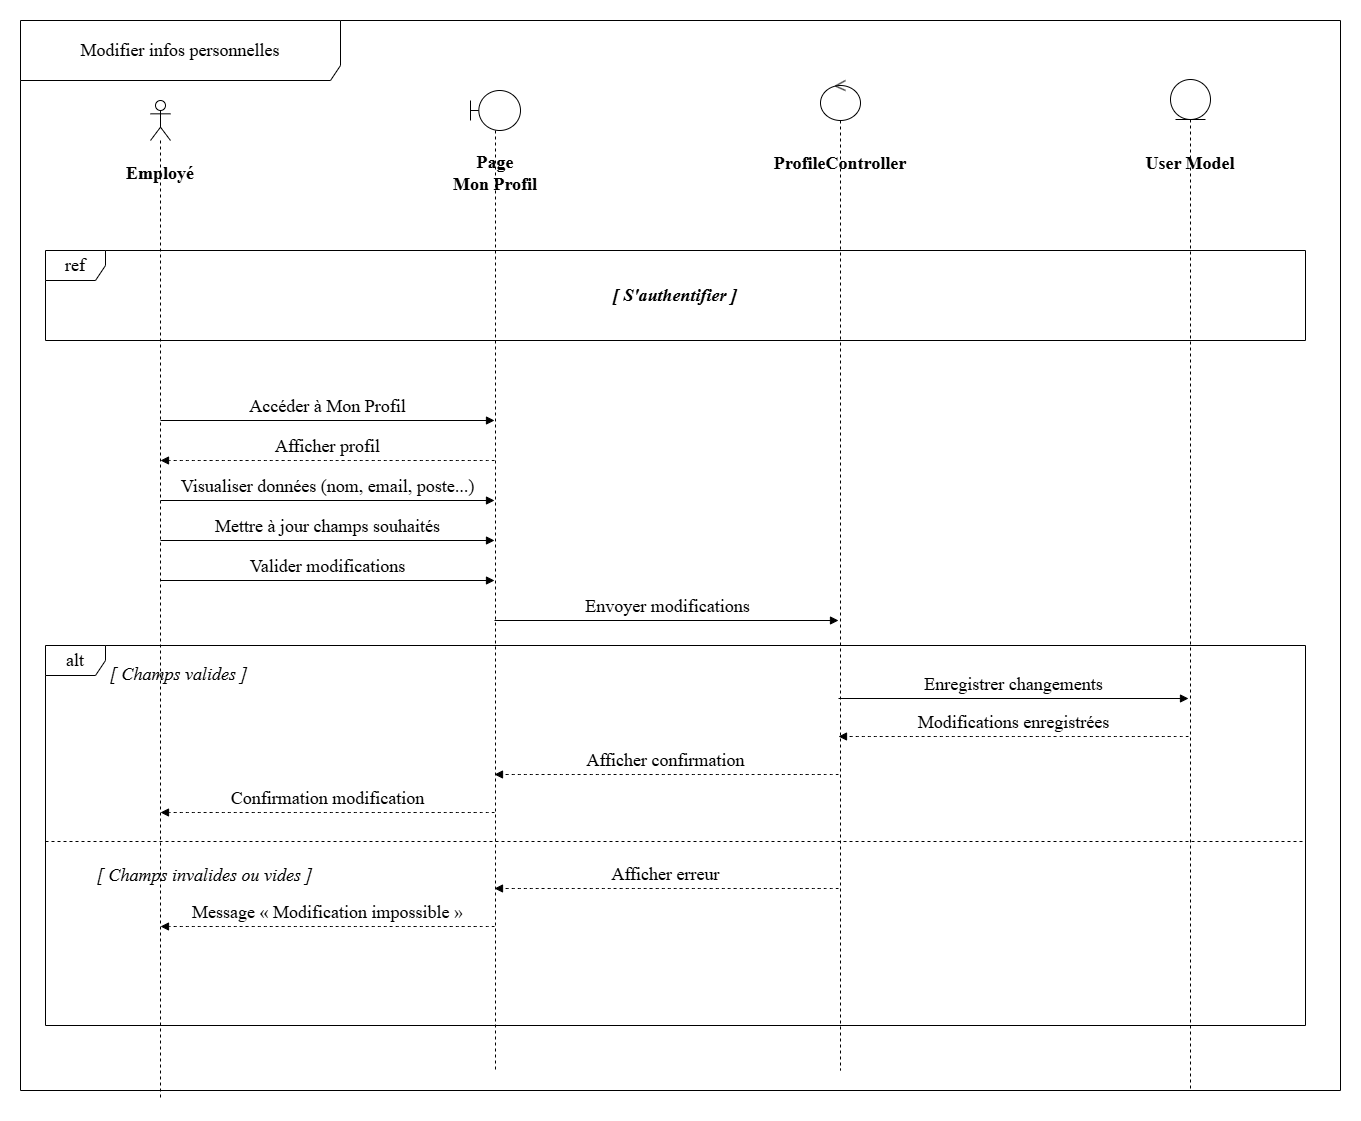
\includegraphics[width=0.85\textwidth]{projet/images/img diag sprint 2/modifier_infos.png}
    \caption{Diagramme de séquence du cas d'utilisation « Modifier infos personnelles »}
\end{figure}

\subsubsection*{Diagramme de séquence du cas d'utilisation « Consulter ses absences »}

Ce diagramme décrit la consultation par l'employé de son historique d'absences et de retards. Il accède à la section dédiée de son tableau de bord, le système interroge la base de données et affiche la liste détaillée des occurrences enregistrées.

\begin{figure}[H]
    \centering
    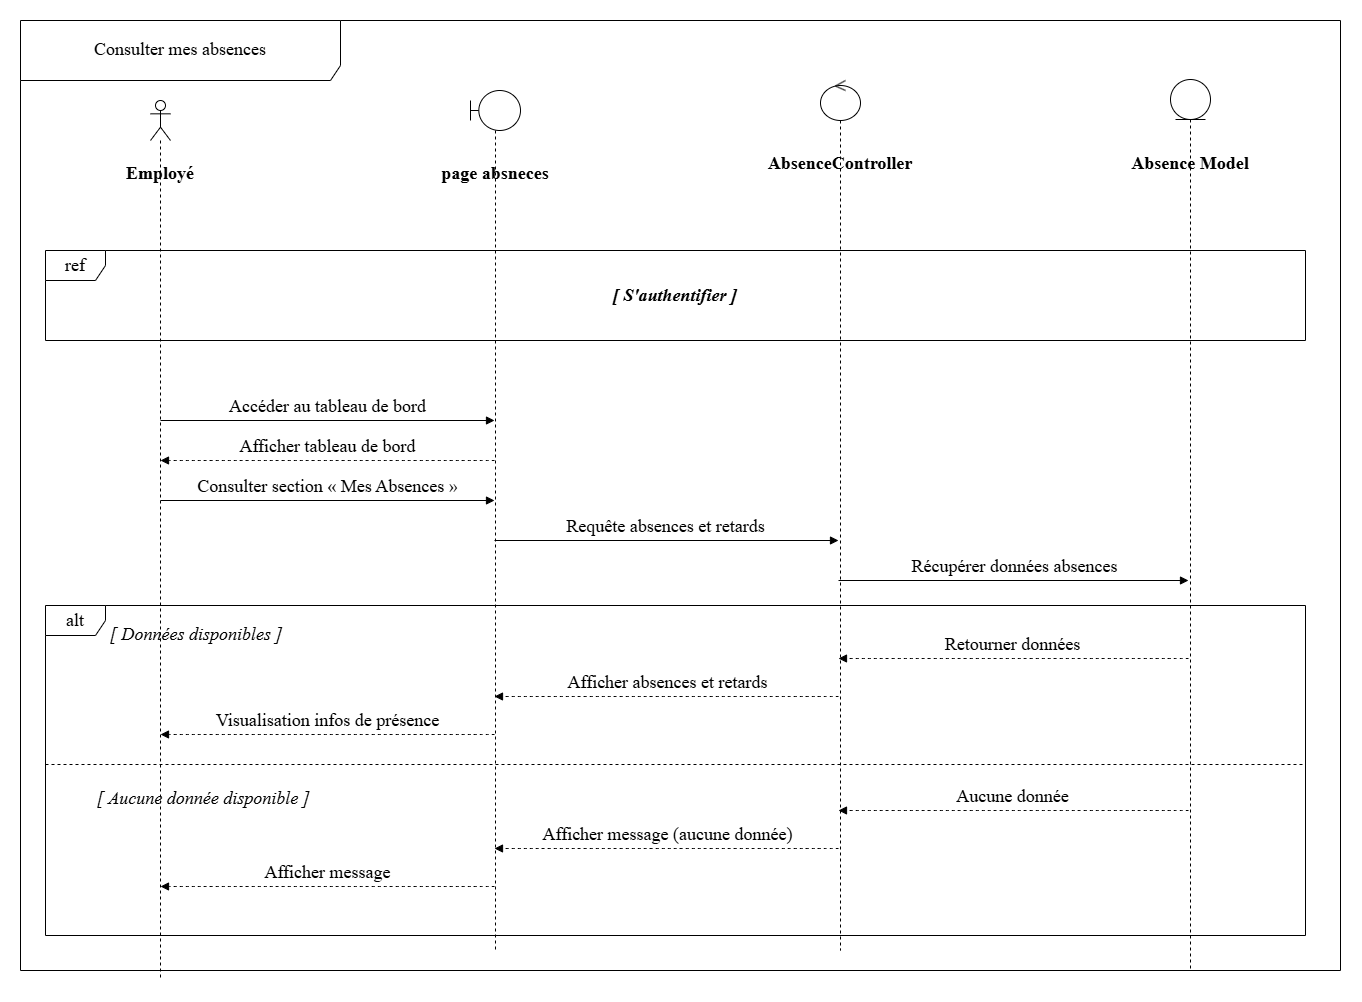
\includegraphics[width=0.85\textwidth]{projet/images/img diag sprint 2/consulter_retard.png}
    \caption{Diagramme de séquence du cas d'utilisation « Consulter ses absences et retards »}
\end{figure}


\subsubsection*{Diagramme de séquence du cas d'utilisation « Pointage facial »}

Le diagramme de pointage facial illustre le processus d'enregistrement de la présence des employés via la reconnaissance faciale, depuis la capture du visage par la caméra jusqu'à la vérification de l'identité et l'enregistrement des heures d'entrée et de sortie dans le système.

\begin{figure}[H]
    \centering
    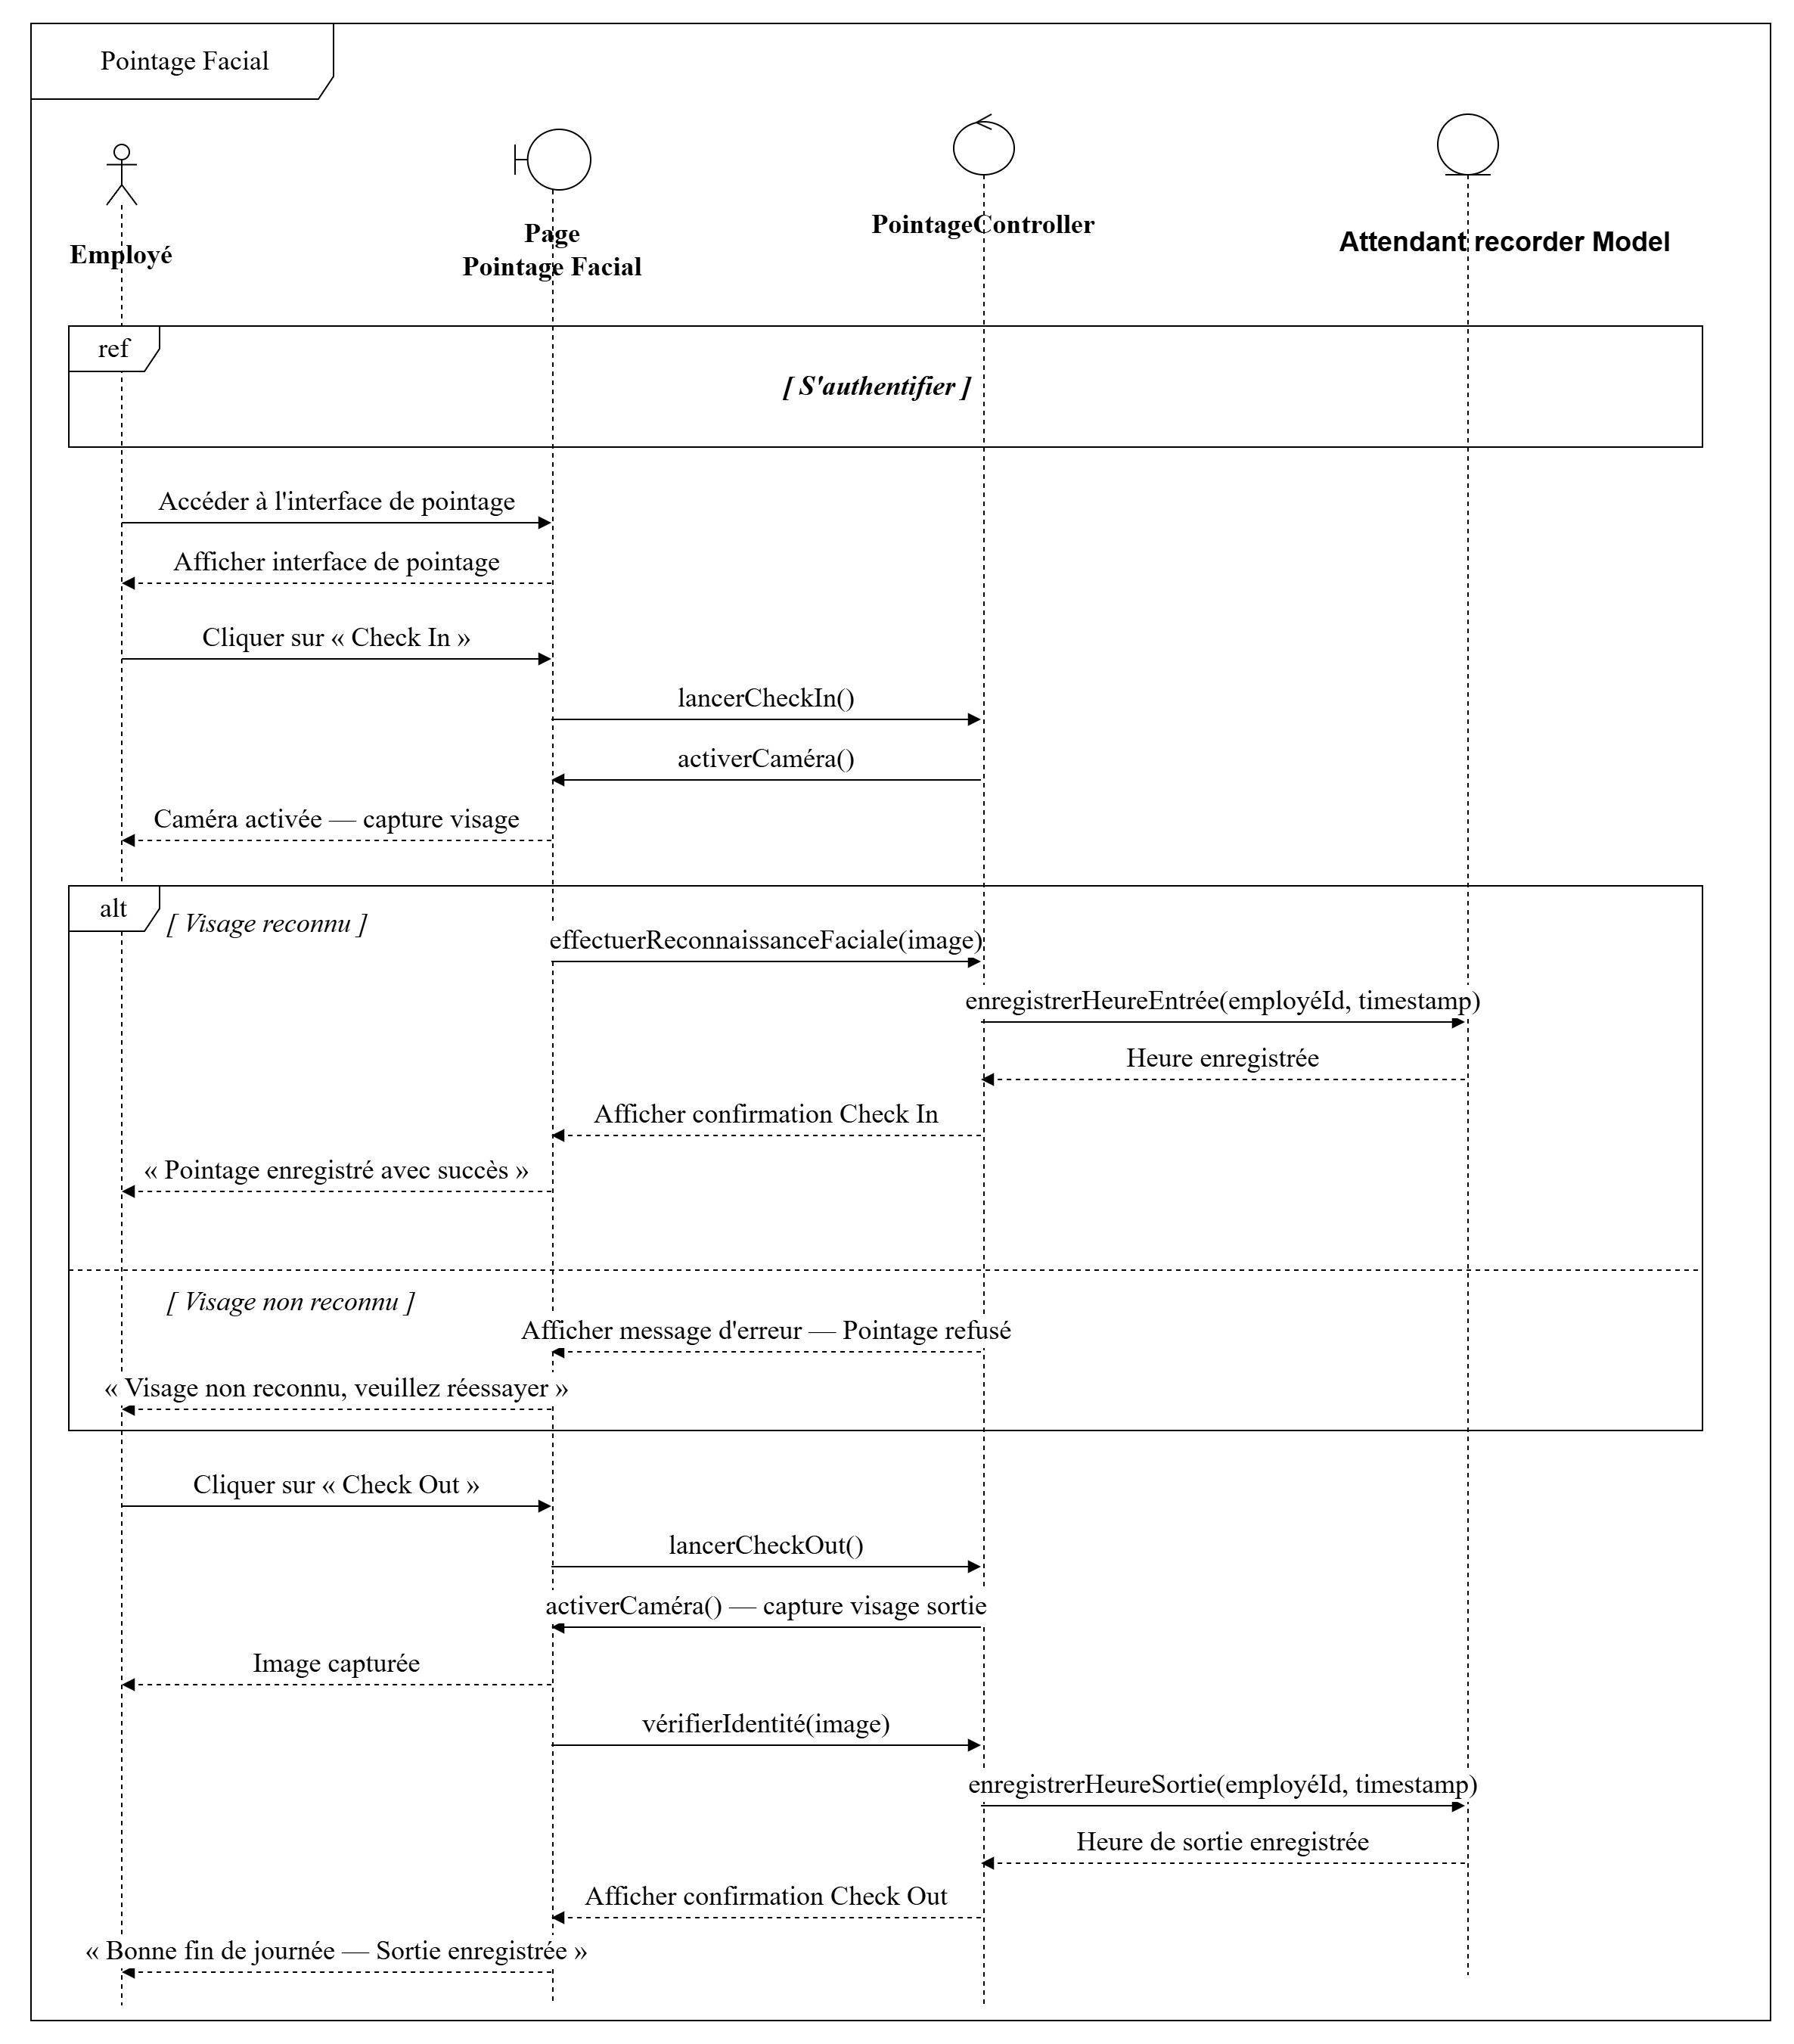
\includegraphics[width=0.85\textwidth]{projet/images/img diag sprint 2/pointage_facial.png}
    \caption{Diagramme de séquence du cas d'utilisation « Pointage facial »}
\end{figure}


\subsubsection{Diagramme de classe du sprint 2}

Ce diagramme de classe illustre la structure des composants liés au pointage intelligent, en montrant les classes Camera, Présence, Absence et leurs attributs respectifs, ainsi que leurs relations avec la classe Employé au sein du système.

\begin{figure}[H]
    \centering
    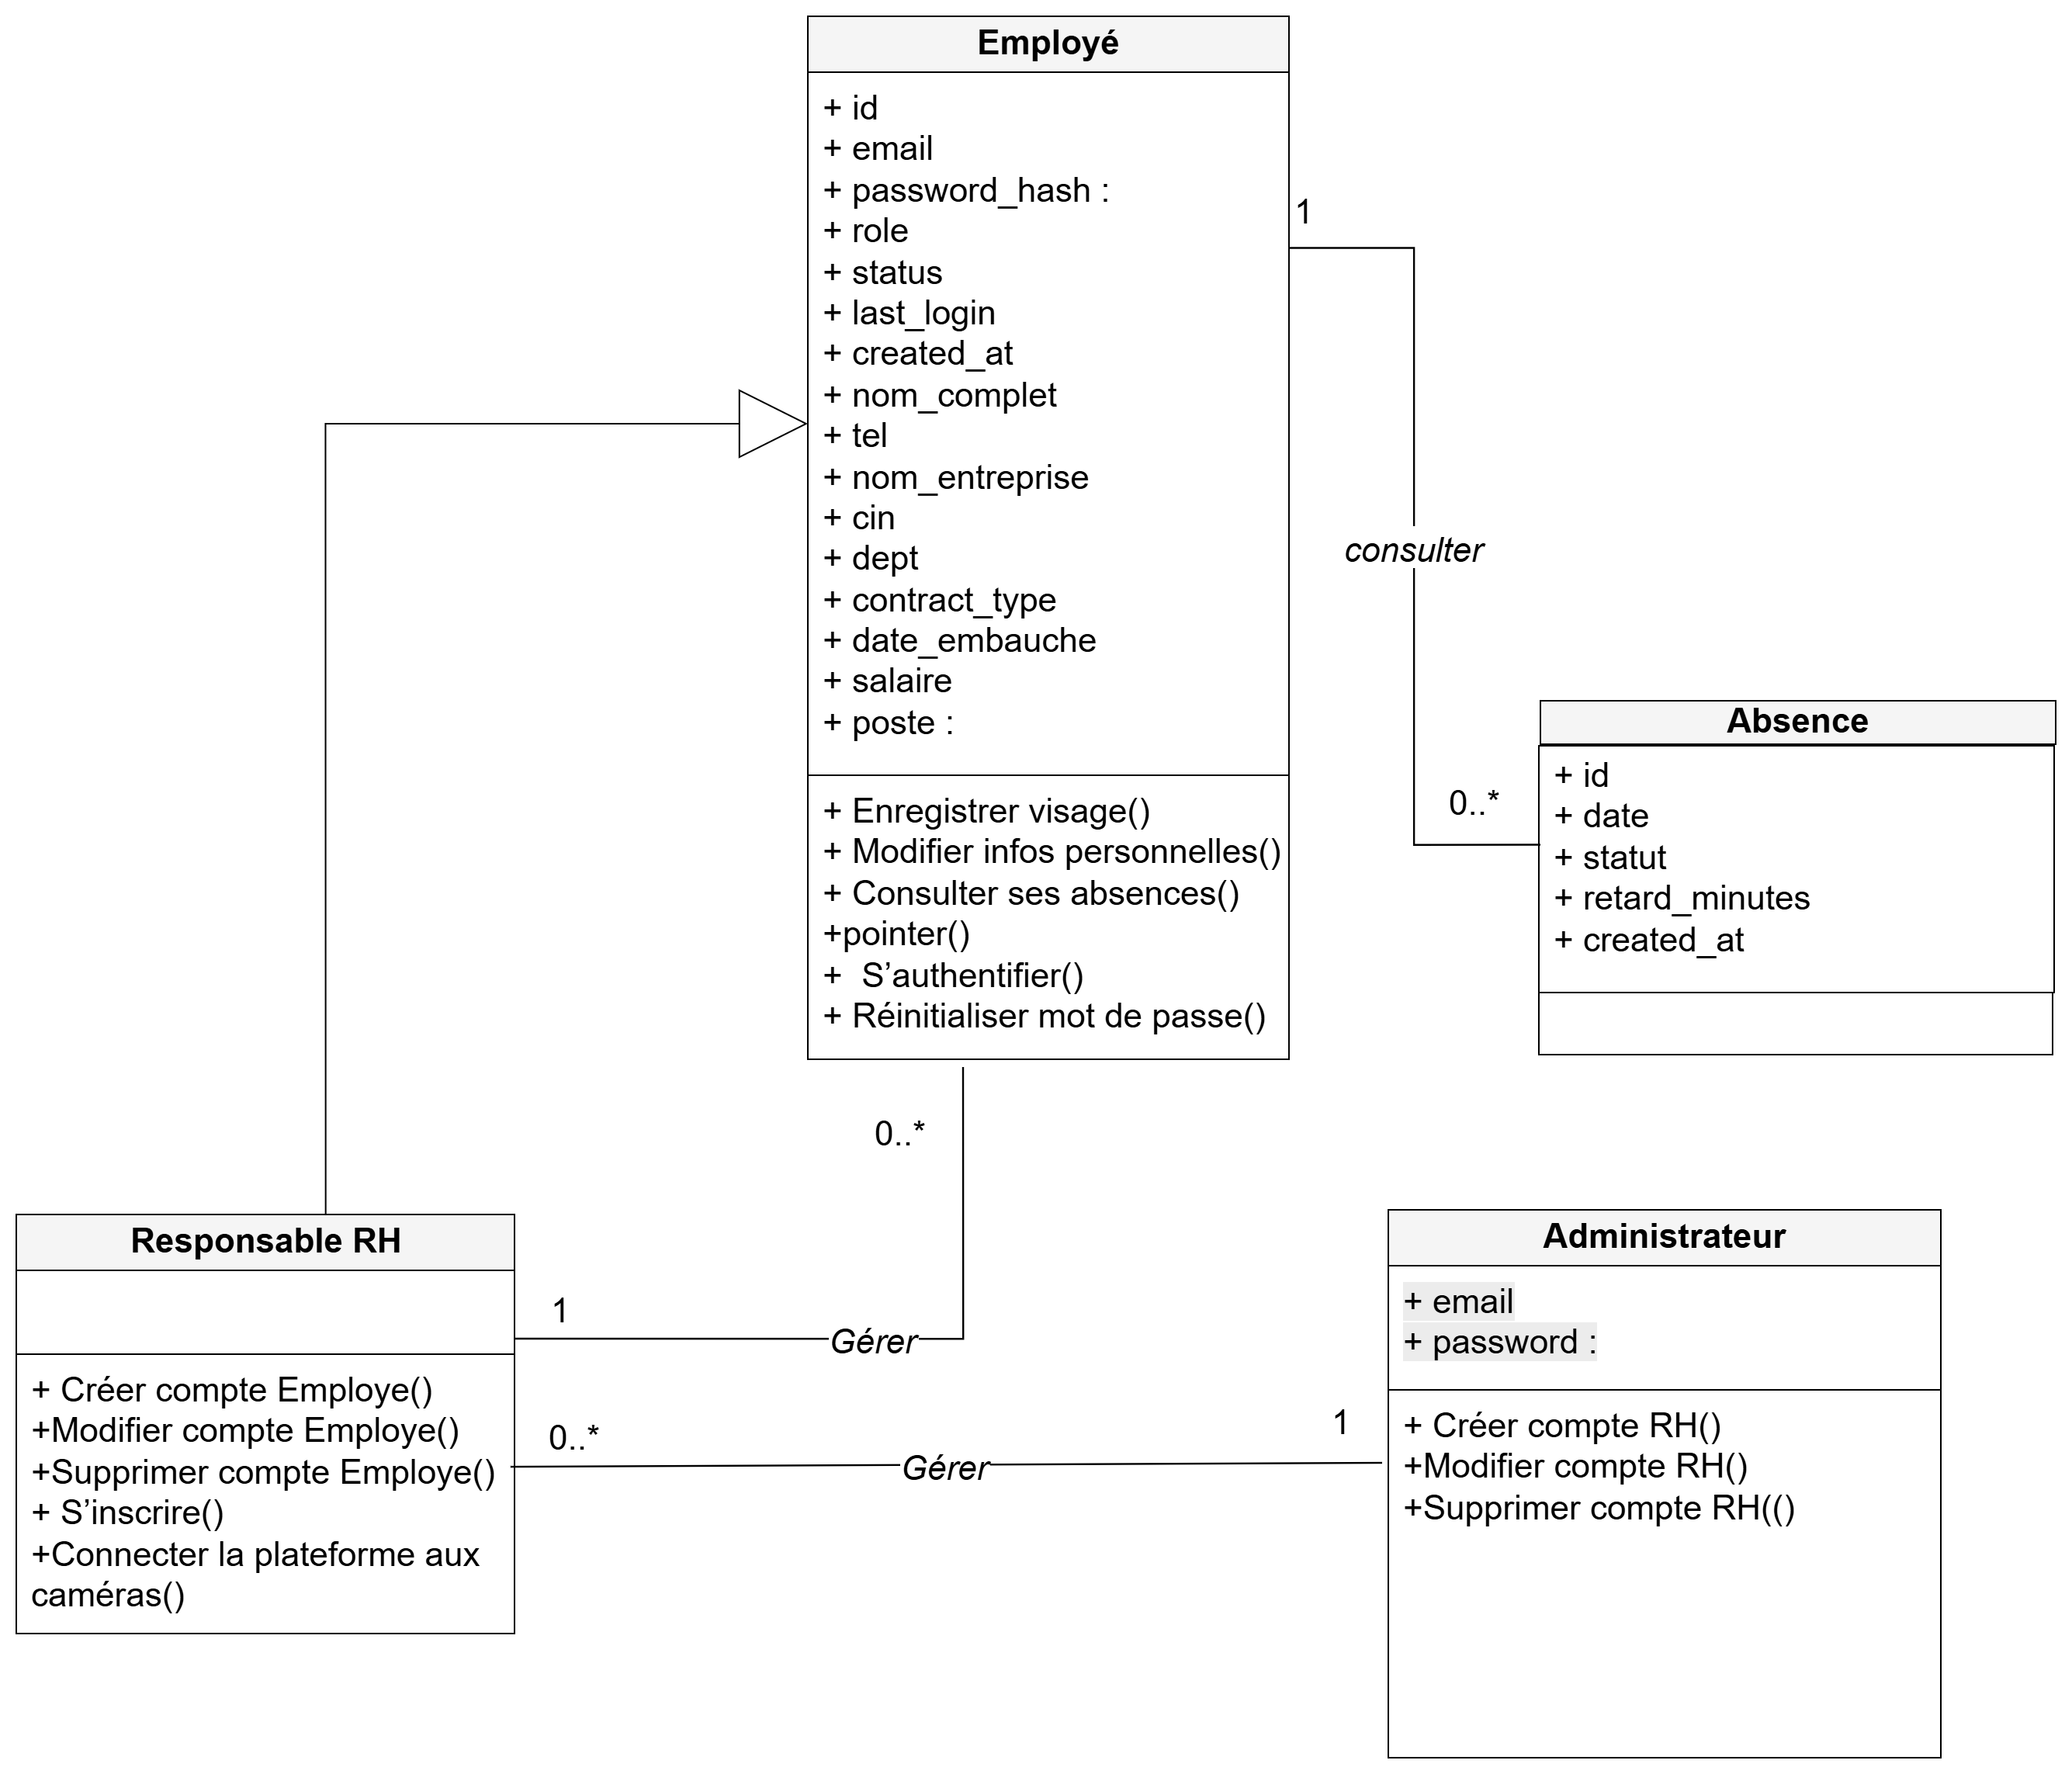
\includegraphics[width=0.85\textwidth]{projet/images/classe finale/daigramme_de_classe_s2.png}
    \caption{Diagramme de classe du sprint 2}
    \label{fig:classe2}
\end{figure}


%============================================================
\subsection{Interfaces réalisées pour le sprint 2}
%============================================================

\subsubsection*{Connecter la plateforme aux caméras}

Cette interface permet de connecter le système aux caméras afin d'activer la capture et la reconnaissance des flux vidéo.

\begin{figure}[H]
    \centering
    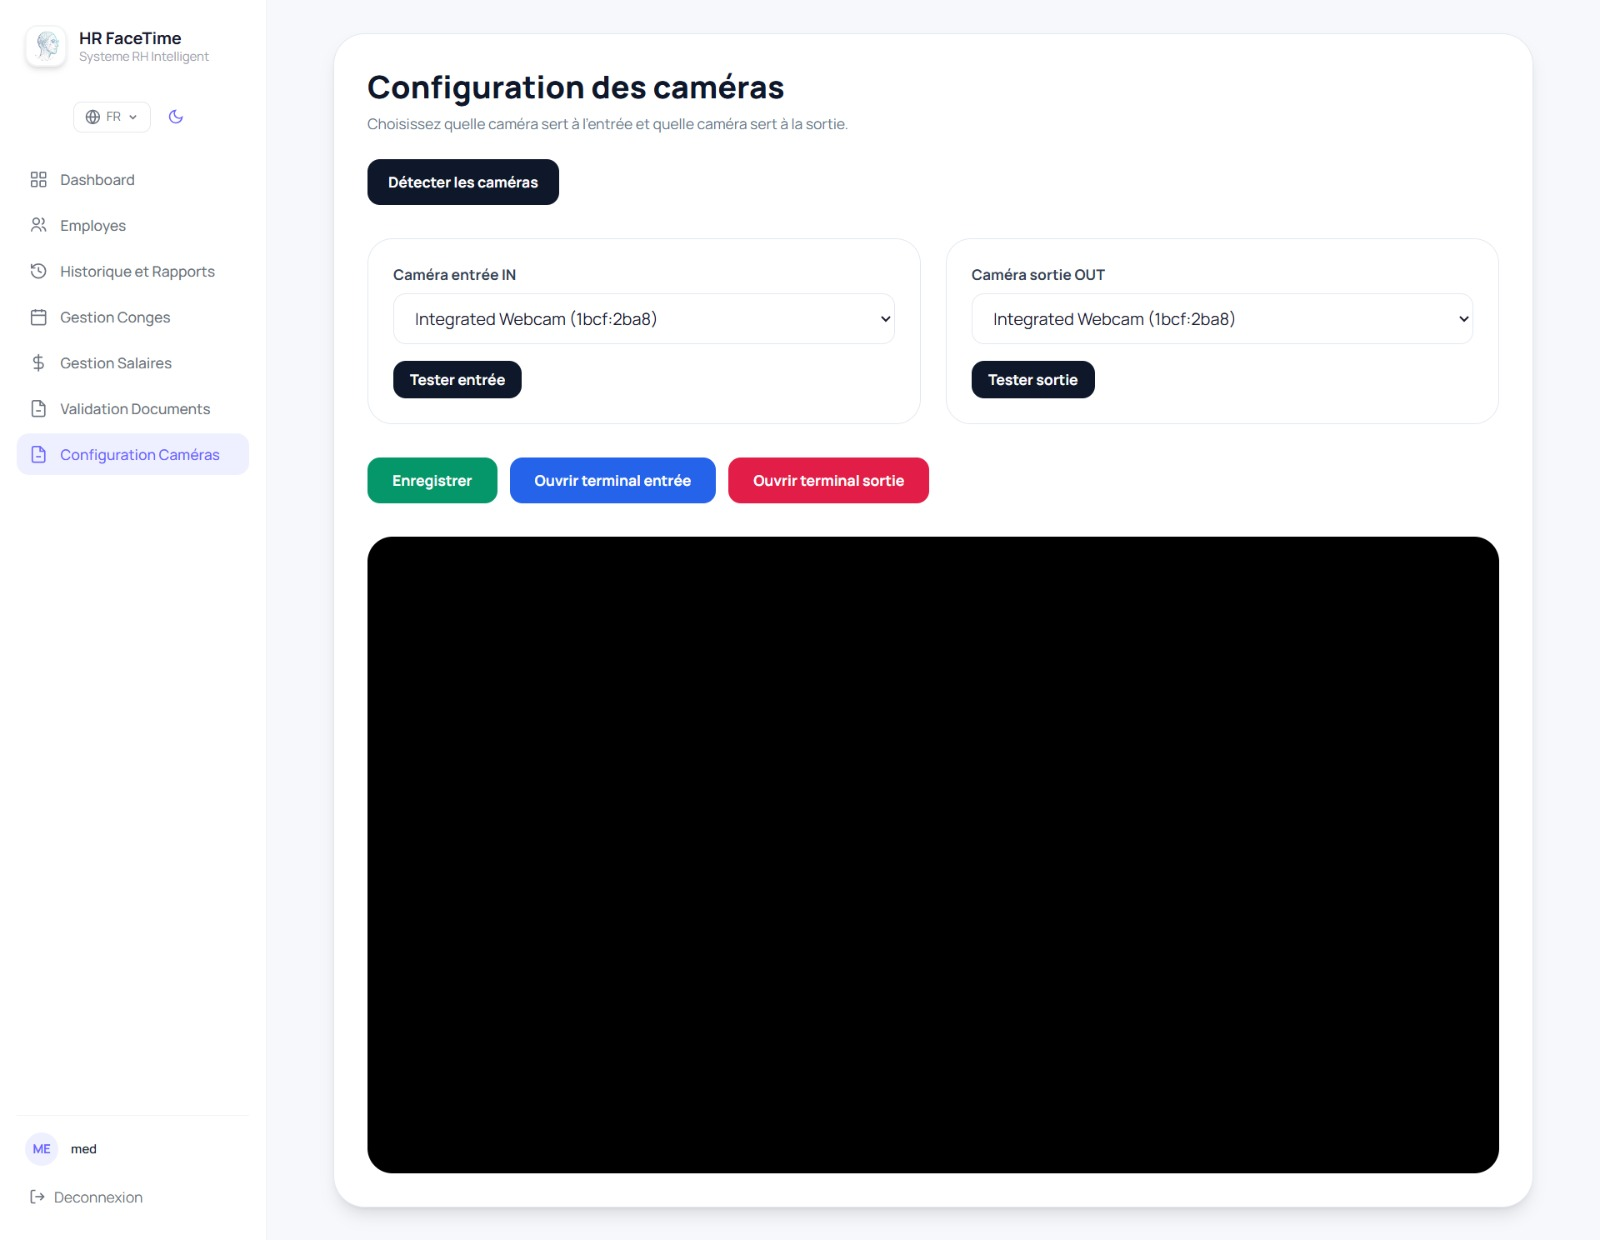
\includegraphics[width=0.9\textwidth]{projet/images/interface/s2/connecter camera.jpeg}
    \caption{Connecter la plateforme aux caméras}
    \label{fig:interface6}
\end{figure}


\subsubsection*{Enregistrer le visage}

Cette interface permet d'enregistrer les données faciales d'un utilisateur pour la reconnaissance et l'identification automatique.

\begin{figure}[H]
    \centering
    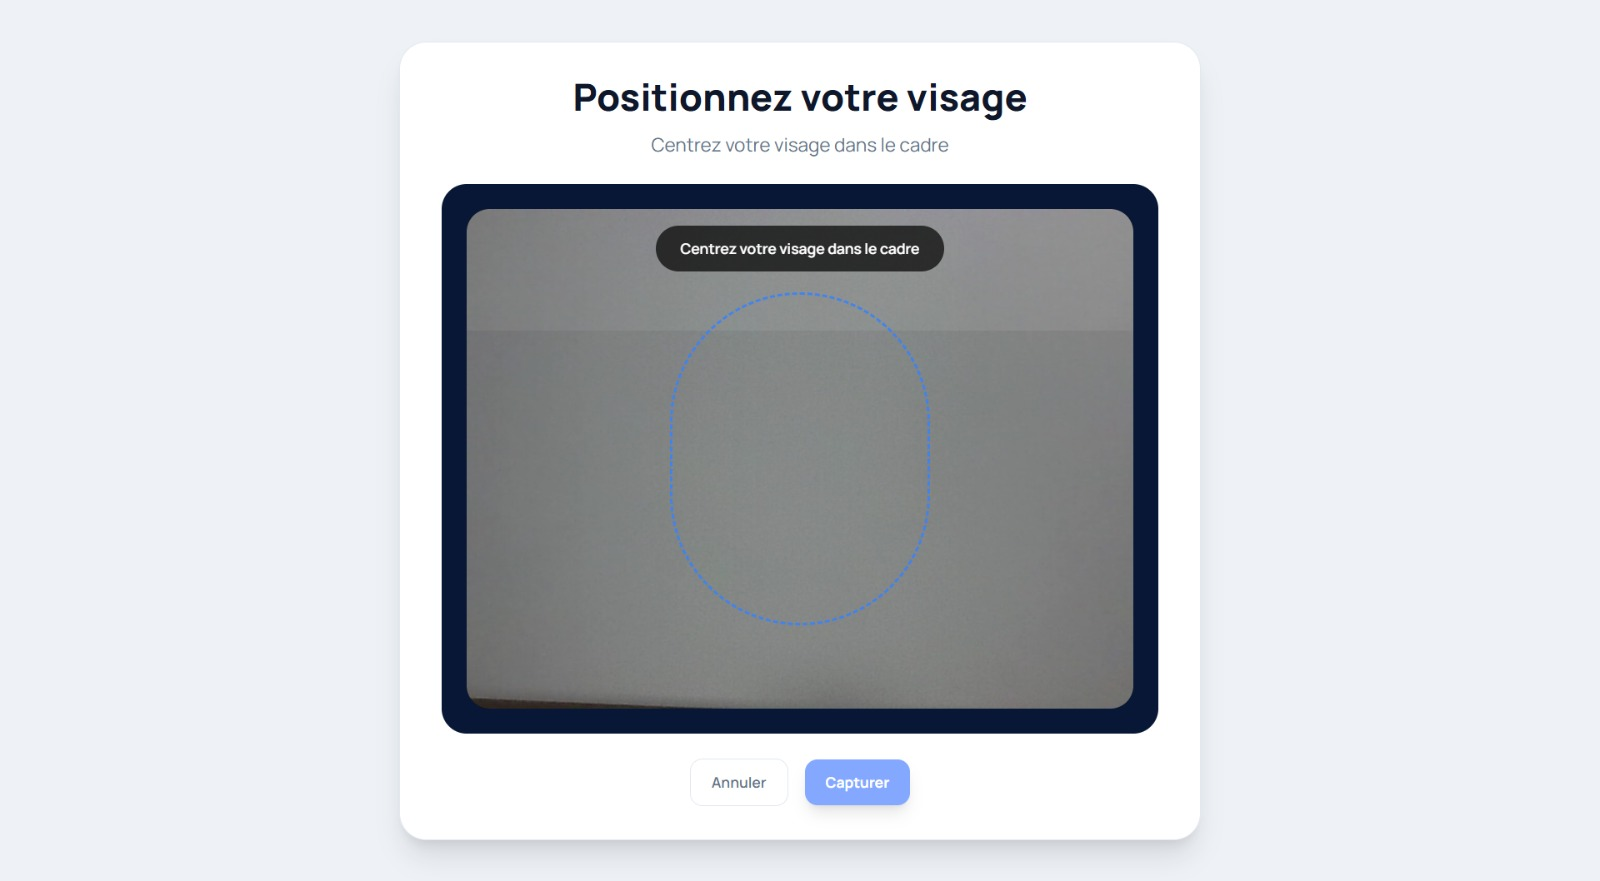
\includegraphics[width=0.9\textwidth]{projet/images/interface/s2/enregister visage.jpeg}
    \caption{Enregistrer le visage}
    \label{fig:interface7}
\end{figure}


\subsubsection*{Modifier infos personnelles}

Cette interface permet à l'utilisateur de modifier ses informations personnelles telles que le nom, l'e-mail ou le mot de passe.

\begin{figure}[H]
    \centering
    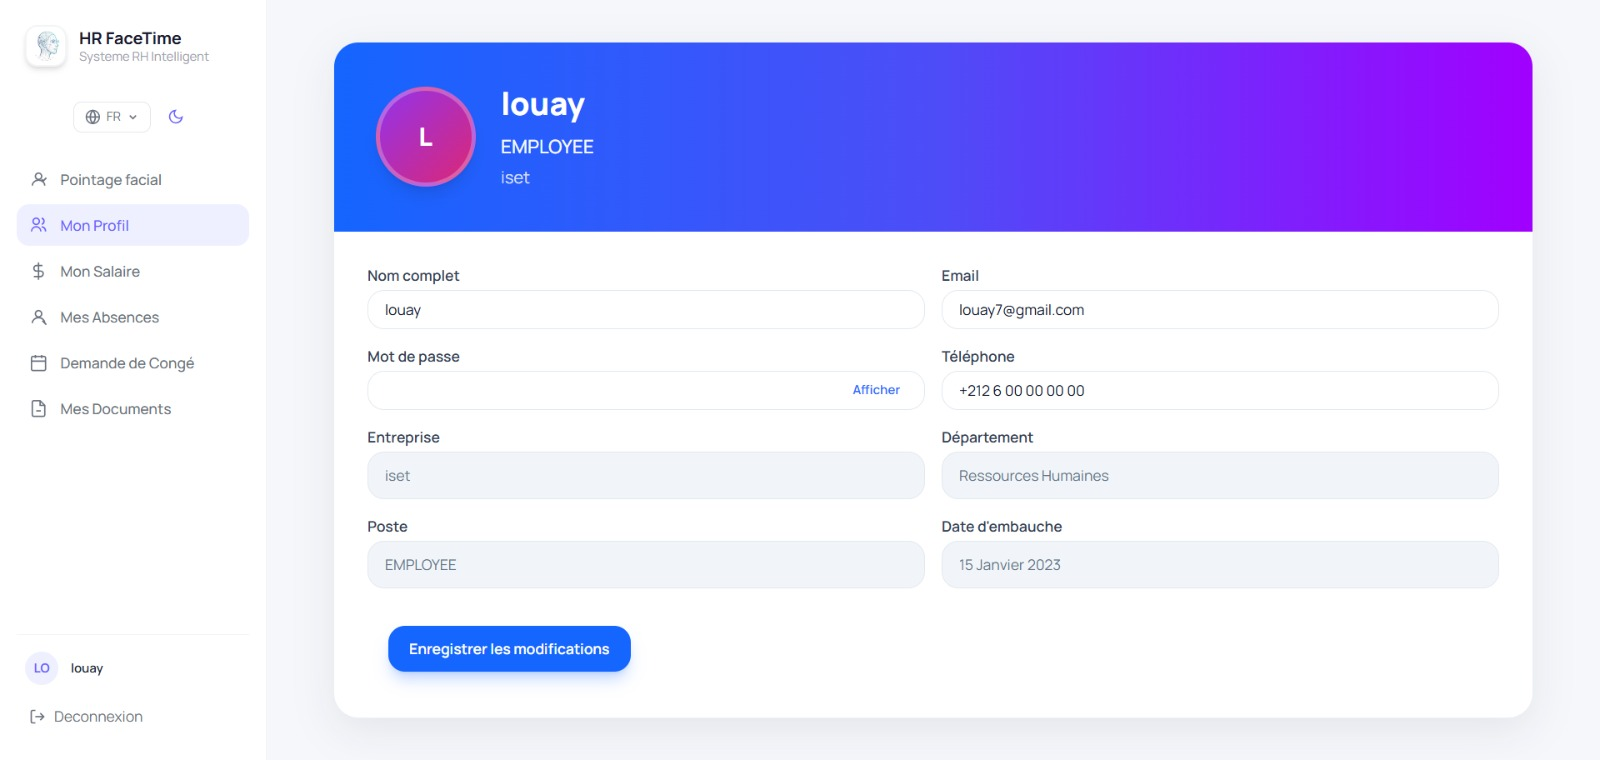
\includegraphics[width=0.9\textwidth]{projet/images/interface/s2/modifier profile.jpeg}
    \caption{Modifier infos personnelles}
    \label{fig:interface8}
\end{figure}


\subsubsection*{Consulter mes absences}

Cette interface permet à l'utilisateur de consulter l'historique et les détails de ses absences enregistrées.

\begin{figure}[H]
    \centering
    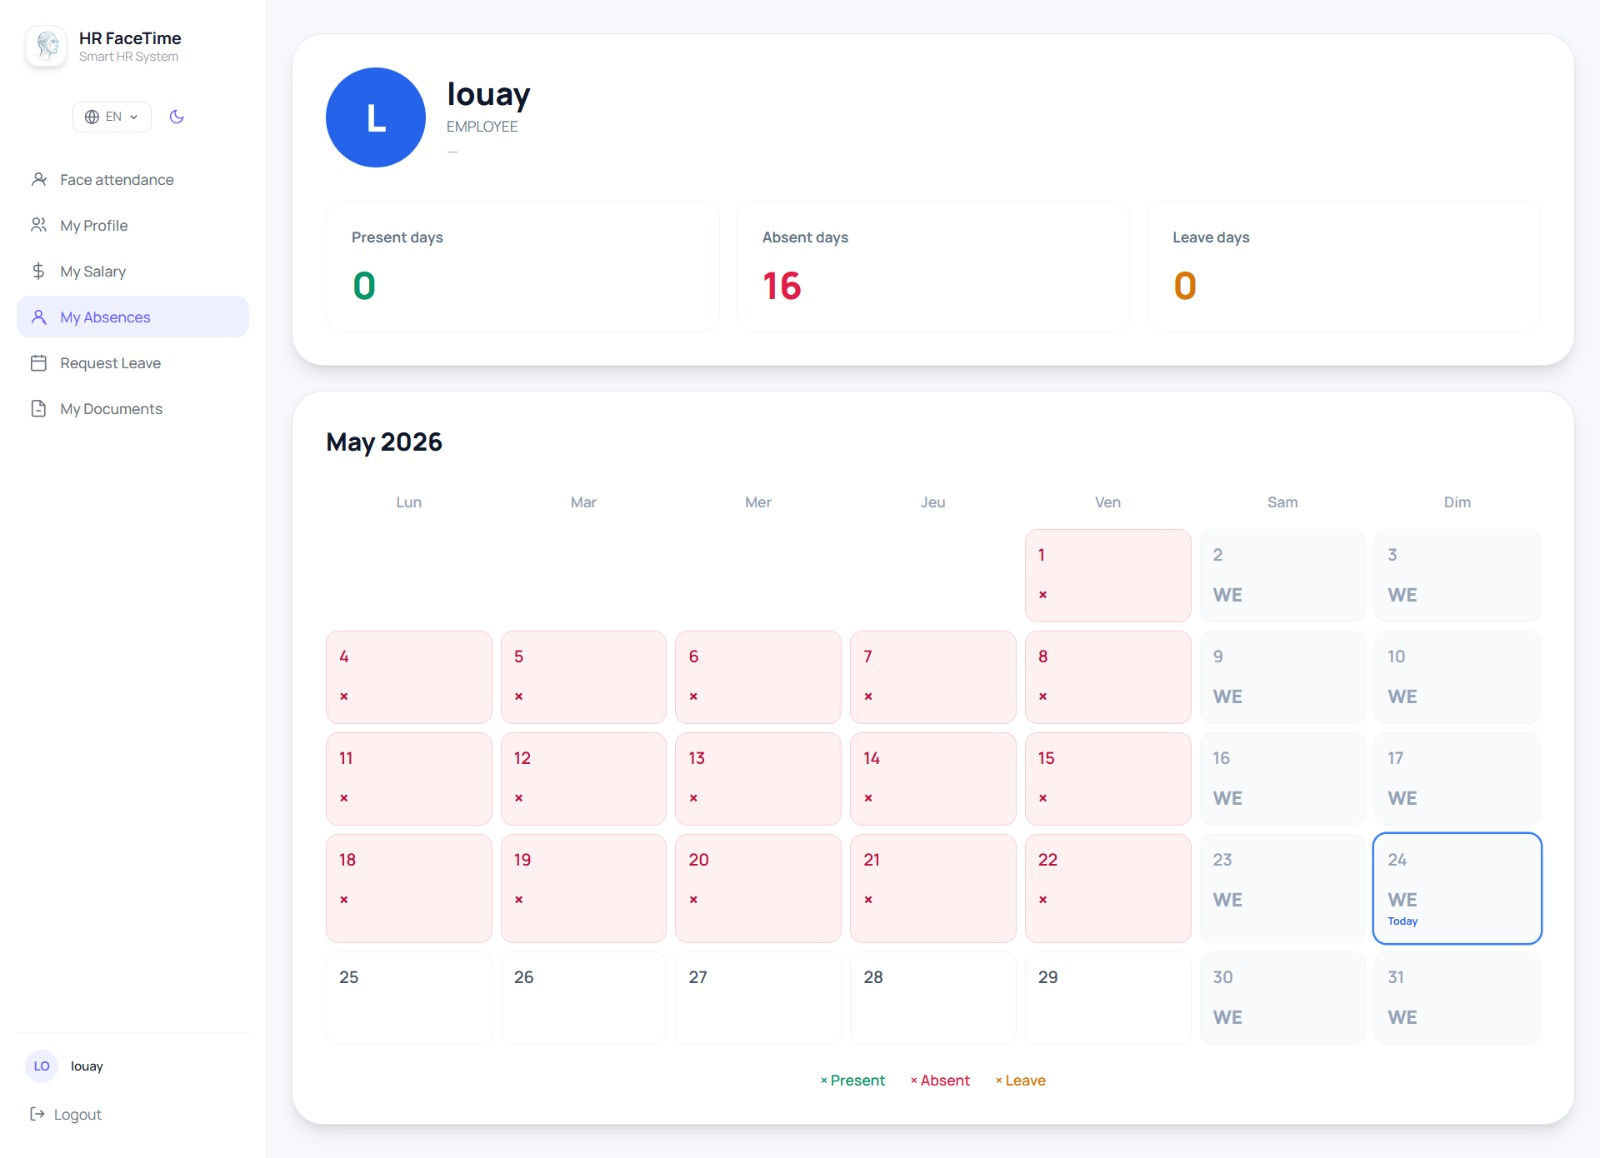
\includegraphics[width=0.9\textwidth]{projet/images/interface/s2/absence.jpeg}
    \caption{Consulter mes absences}
    \label{fig:interface9}
\end{figure}


\subsubsection*{Interface de pointage facial}

L'interface de pointage facial permet aux employés d'enregistrer automatiquement leur présence et leur départ via la reconnaissance faciale.

\begin{figure}[H]
    \centering
    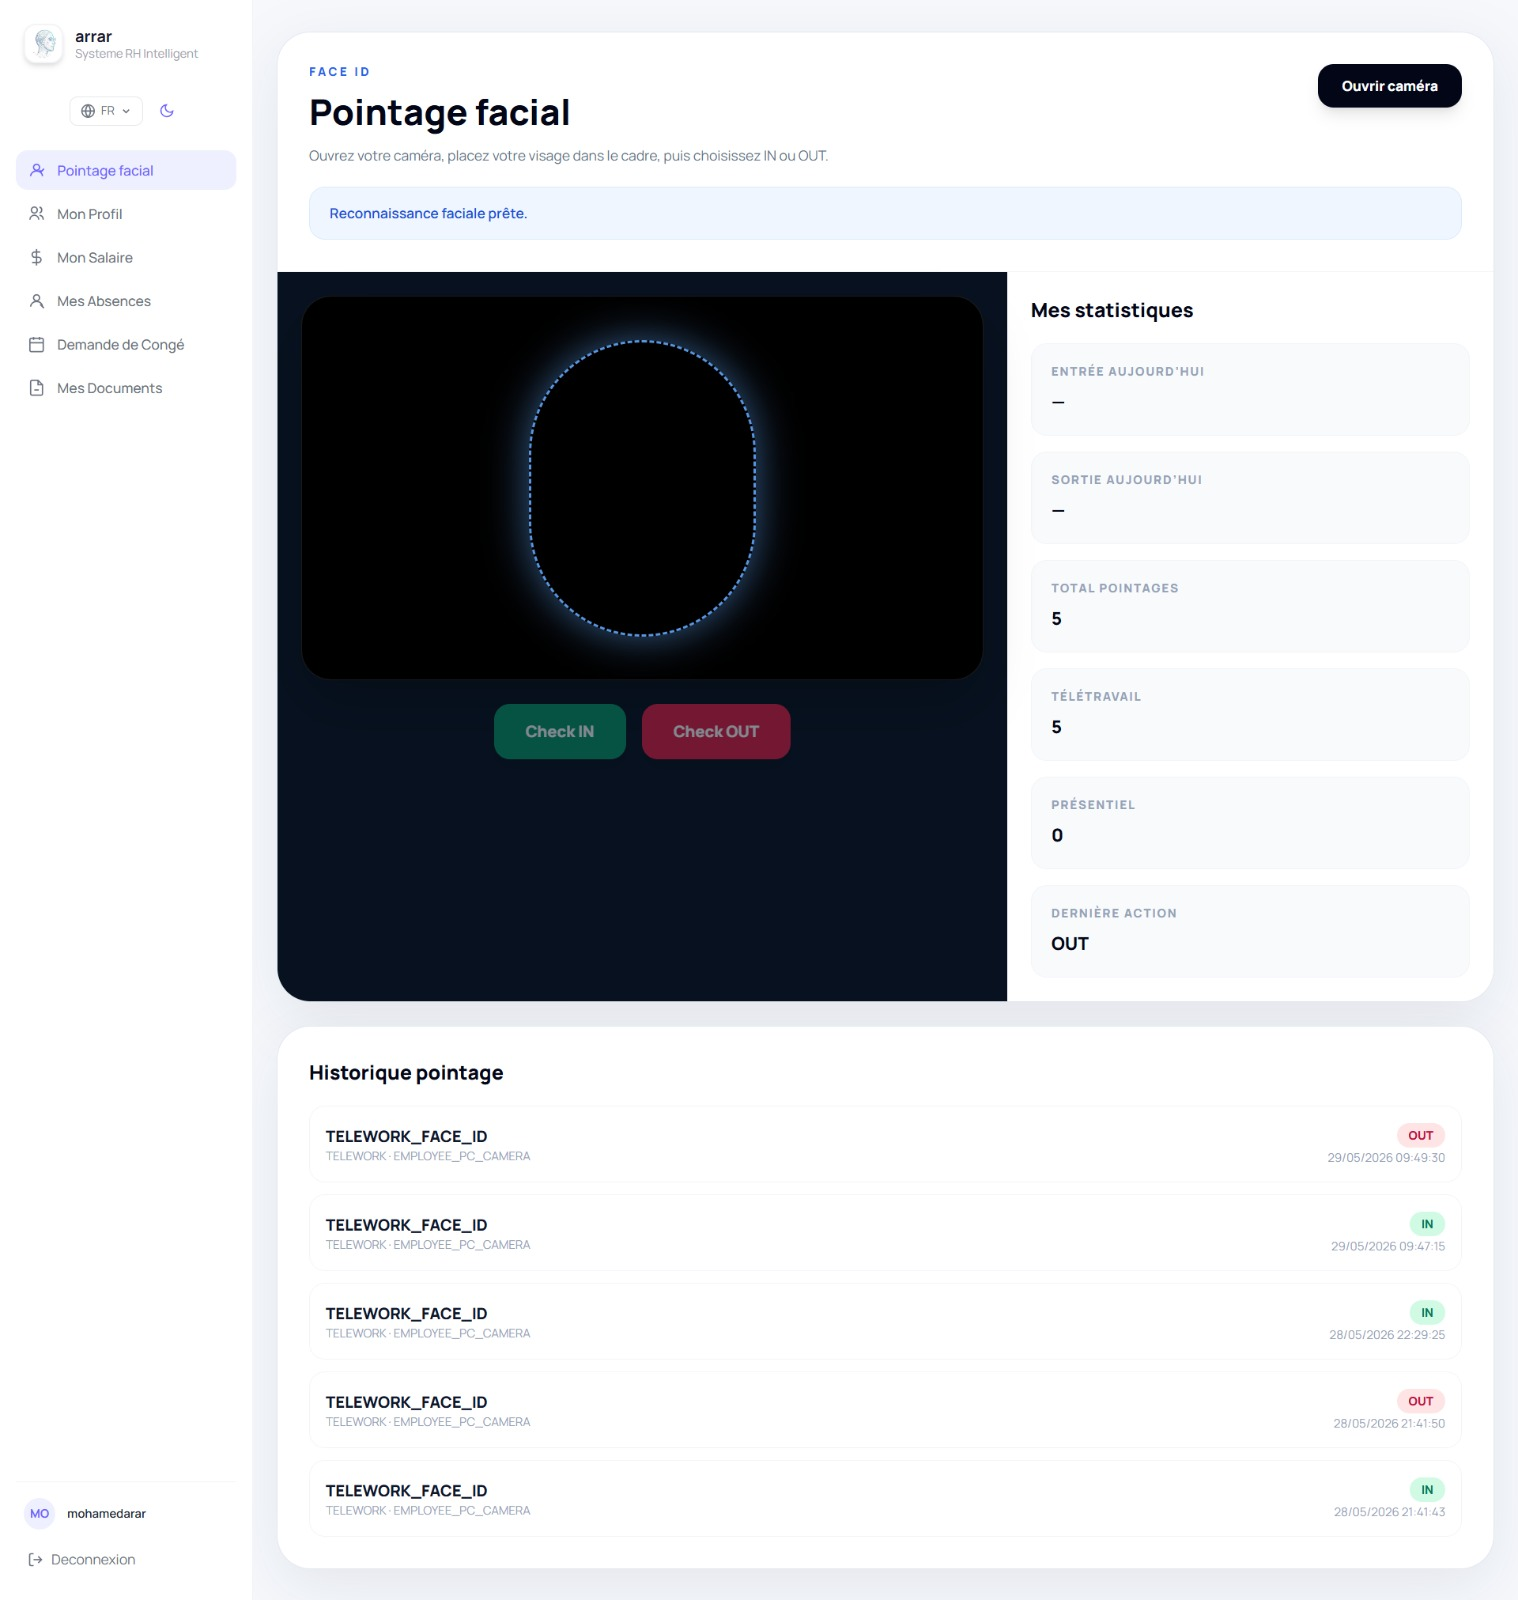
\includegraphics[width=0.9\textwidth]{projet/images/interface/s2/pointage_facial.jpeg}
    \caption{Interface de pointage facial}
    \label{fig:pointage_facial}
\end{figure}


%============================================================
\section{Conclusion}
%============================================================

Cette première release établit les bases essentielles du système en assurant une authentification sécurisée et une gestion efficace des comptes des différents acteurs. Elle intègre également la gestion des employés ainsi qu'un système de pointage intelligent basé sur la reconnaissance faciale, permettant un suivi précis des présences, absences et retards, et offrant au Responsable RH un meilleur contrôle de l'assiduité du personnel.

\chapter{Release 2} 

\newpage

\section{Introduction}
Ce chapitre est un élément clé dans la réalisation du projet, connu sous le nom de Release 2.
La sortie de cette version donne le produit final.

\section{Sprint 3: Gestion  des Congés et des Documents Administratifs}

Ce sprint vise à développer les fonctionnalités de gestion des ressources humaines, notamment la gestion des congés, des documents administratifs, des primes et des salaires afin d'optimiser le suivi des employés et les processus RH.

\subsection{Objectif de sprint 3}
L'objectif de ce sprint est de développer les fonctionnalités liées
à la gestion des congés, documents,
primes et salaires, ainsi que la validation, le rejet et le dépôt des documents.

\subsection{Durée de sprint 3}
\begin{itemize}
    \item \textbf{Date de début du sprint} : 07/04/2026
    \item \textbf{Date de fin du sprint} : 02/05/2026
\end{itemize}

\subsection{Backlog de sprint 3}
Le  backlog du sprint relatif à ce sprint est représenté dans le tableau ci-joint.
\begin{longtable}{|>{\centering\arraybackslash}m{0.5cm}|
    >{\centering\arraybackslash}m{3cm}|
    >{\centering\arraybackslash}m{2.5cm}|
    >{\centering\arraybackslash}m{3cm}|
    >{\centering\arraybackslash}m{3cm}|
    >{\centering\arraybackslash}m{0.7cm}|
    >{\centering\arraybackslash}m{0.9cm}|}
\hline
\textbf{ID} & \textbf{User Story} & \textbf{En tant que} & \textbf{Je veux} & \textbf{Afin de} & \textbf{P} & \textbf{C} \\
\hline
11 & Valider congé & Responsable RH & valider une demande de congé & autoriser l'absence & 5 & 2 \\ \hline
12 & Refuser congé & Responsable RH & refuser une demande de congé & gérer les absences & 5 & 2 \\ \hline
13 & Attribuer prime & Responsable RH & attribuer une prime à un employé & récompenser les employés & 3 & 2 \\ \hline
14 & Attribuer déduction & Responsable RH & appliquer une déduction à un employé & gérer la paie avec précision & 4 & 3 \\ \hline
15 & Mettre à jour status salaire & Responsable RH & mettre à jour le statut du salaire & assurer la paie & 5 & 3 \\ \hline
16 & Consulter documents & Responsable RH & consulter les documents envoyés & vérifier les pièces & 3 & 2 \\ \hline
17 & Valider document & Responsable RH & valider un document & contrôler les absences & 4 & 2 \\ \hline
18 & Rejeter document & Responsable RH & rejeter un document & contrôler les absences & 4 & 2 \\ \hline
19 & Modifer salaire & Responsable RH & modifier un salaire à un employé & assurer une gestion correcte de la paie & 3 & 3 \\ \hline
25 & Consulter primes & Employé & consulter mes primes & connaître mes avantages & 2 & 1 \\ \hline
26 & Consulter déductions & Employé & voir mes déductions & comprendre ma paie & 2 & 1 \\ \hline
27 & Consulter salaire & Employé & voir mon salaire & vérifier paiement & 3 & 1 \\ \hline
28 & Demande congé & Employé & envoyer une demande & obtenir une absence & 5 & 2 \\ \hline
29 & Déposer document & Employé & déposer un document & justifier une absence & 4 & 3 \\ \hline
\caption{Backlog Sprint 3}
\end{longtable}

\subsection{Spécification fonctionnelle détaillée}

\begin{itemize}

\item \textbf{Diagramme de cas d'utilisation du sprint 3}

\begin{figure}[H]
    \centering
    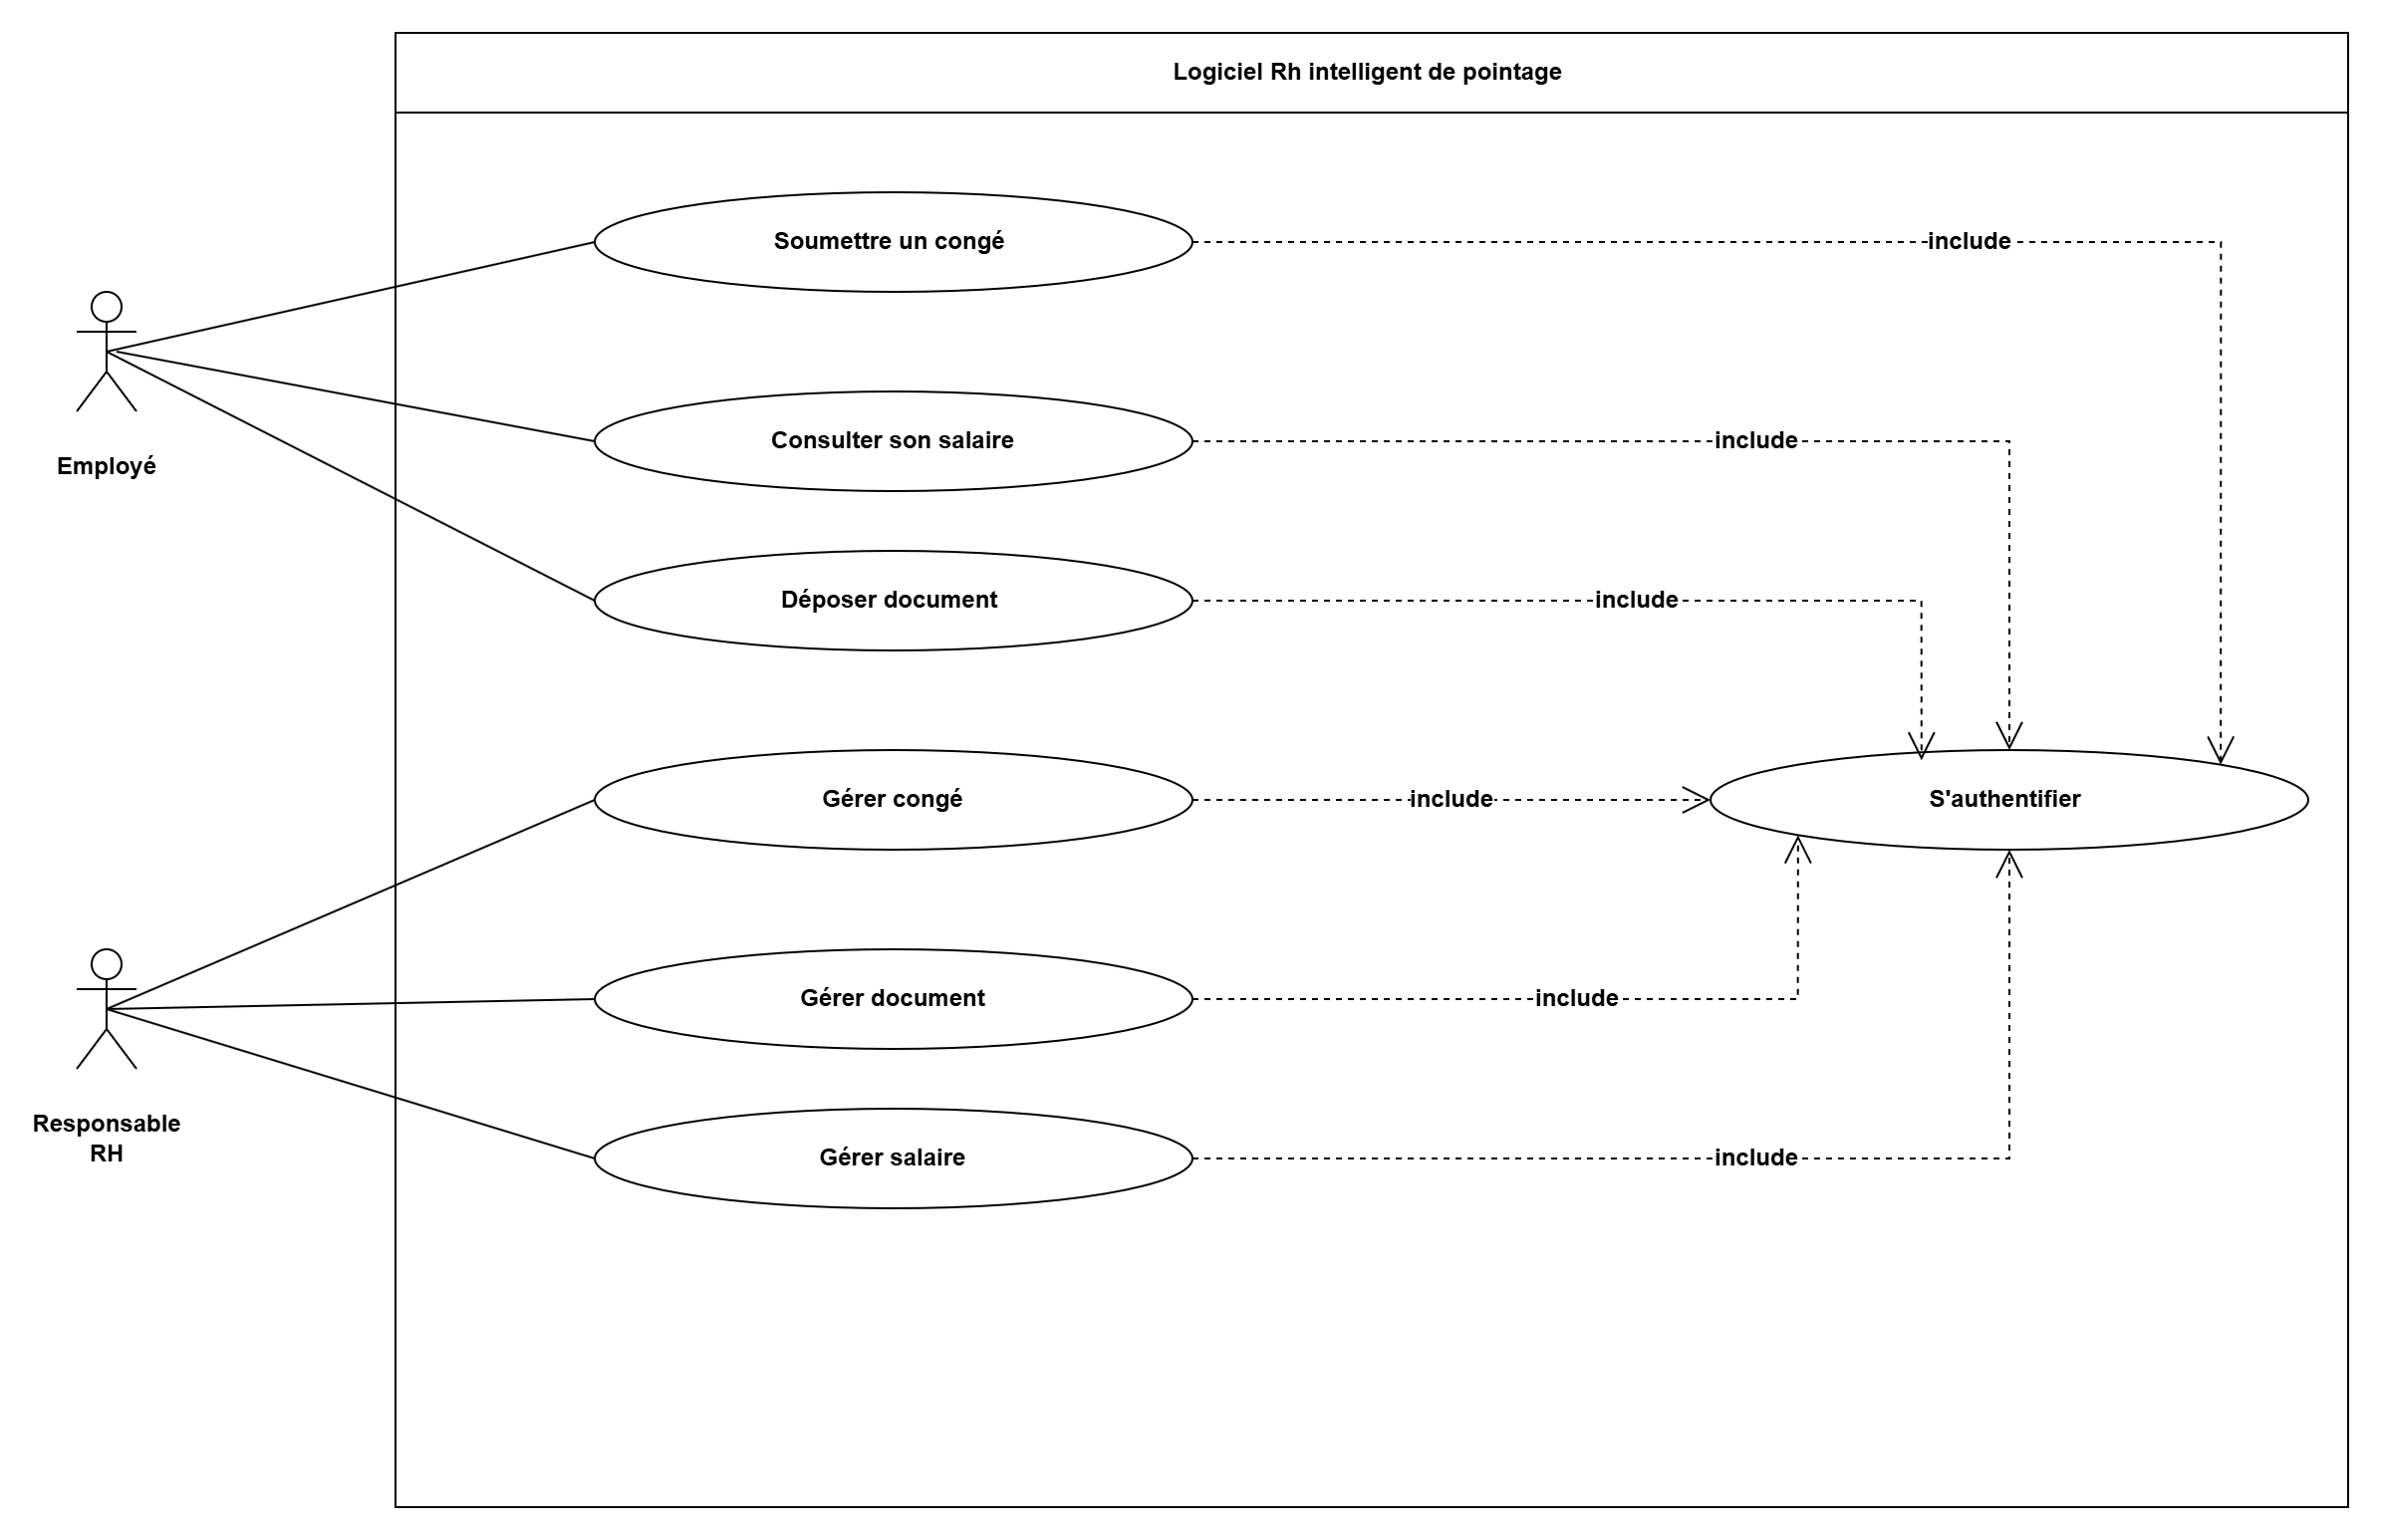
\includegraphics[width=0.9\textwidth]{projet/images/usecase/sprint 3/use_case_s3.png}
    \caption{Diagramme de Cas d'utilisation du Sprint 3}
    \label{fig:usecase_sprint3}
\end{figure}

\item \textbf{Raffinement du cas d'utilisation "Gérer congé"}

\begin{figure}[H]
    \centering
    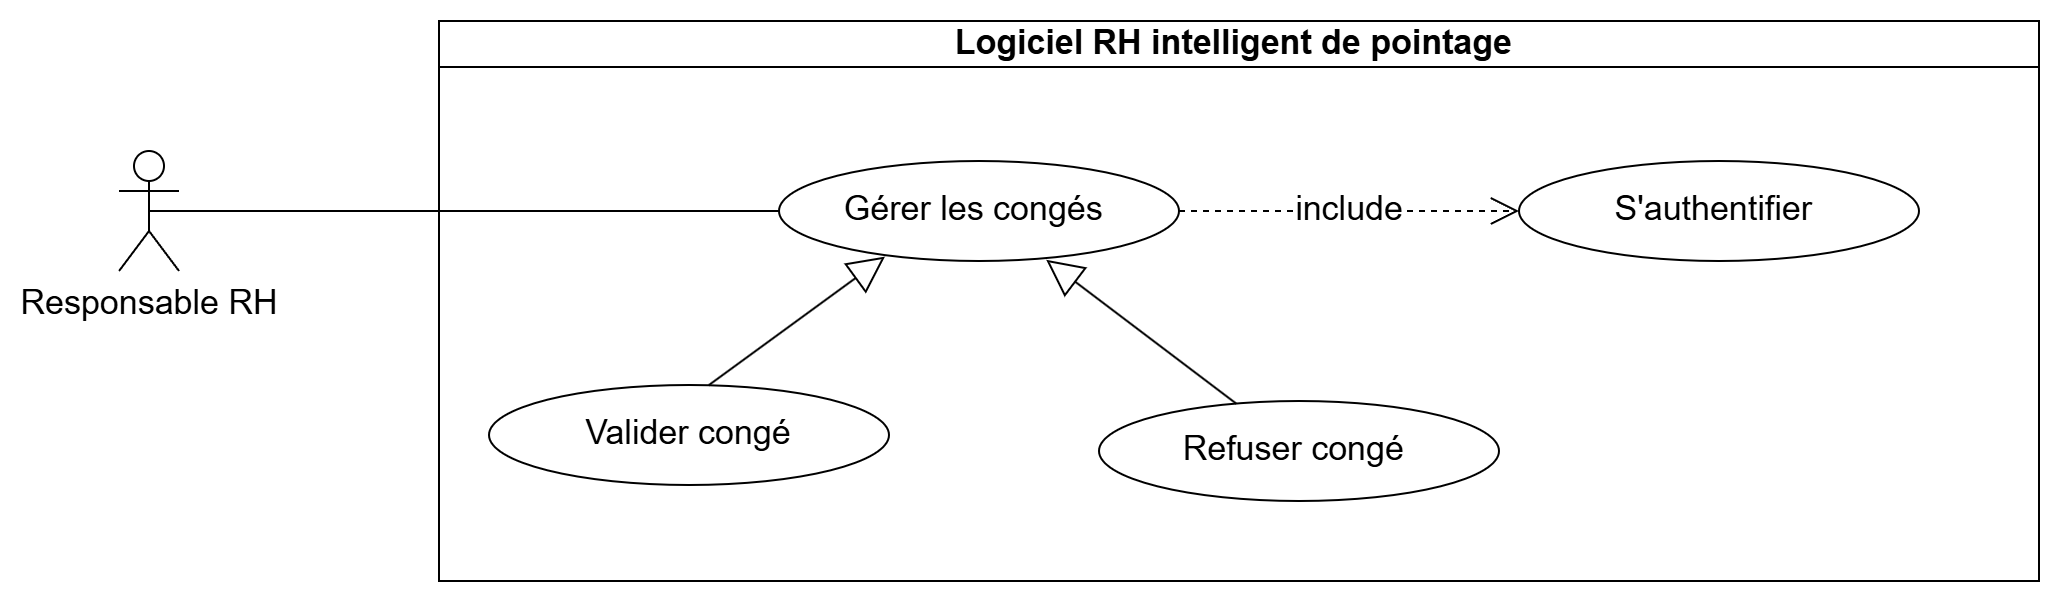
\includegraphics[width=0.9\textwidth]{projet/images/usecase/sprint 3/raffinement_gerer_conges.png}
    \caption{Raffinement du cas d'utilisation "Gérer les congés"}
    \label{fig:raffinement_gerer_conge}
\end{figure}

\item \textbf{Description textuelle : cas d'utilisation «~Valider congé~»}

\begin{center}
\begin{longtable}{|p{5cm}|p{11cm}|}
\hline
\textbf{Nom du cas d'utilisation} & Valider congé \\ \hline
\textbf{Acteurs} & Responsable RH \\ \hline
\textbf{Objectif} & Valider une demande de congé \\ \hline
\textbf{Préconditions} & Le responsable RH doit être authentifié \\ \hline
\textbf{Scénario nominal} &
1. Le responsable RH accède à la liste des demandes. \newline
2. Il sélectionne une demande. \newline
3. Il clique sur "Valider". \newline
4. Le système met à jour le statut de la demande. \\ \hline
\textbf{Scénario d'exception} & Si la demande n'existe pas, le système affiche une erreur. \\ \hline
\textbf{Post-condition} & La demande est validée. \\ \hline
\caption{Description textuelle du cas d'utilisation «~Valider congé~»}
\end{longtable}
\end{center}

\item \textbf{Description textuelle : cas d'utilisation «~Refuser congé~»}

\begin{center}
\begin{longtable}{|p{5cm}|p{11cm}|}
\hline
\textbf{Nom du cas d'utilisation} & Refuser congé \\ \hline
\textbf{Acteurs} & Responsable RH \\ \hline
\textbf{Objectif} & Refuser une demande de congé \\ \hline
\textbf{Préconditions} & Le responsable RH doit être authentifié \\ \hline
\textbf{Scénario nominal} &
1. Le responsable RH accède à la liste des demandes. \newline
2. Il sélectionne une demande. \newline
3. Il clique sur "Refuser". \newline
4. Il saisit un motif. \newline
5. Le système met à jour le statut. \\ \hline
\textbf{Scénario d'exception} & Si aucun motif n'est saisi, le système affiche une erreur. \\ \hline
\textbf{Post-condition} & La demande est refusée. \\ \hline
\caption{Description textuelle du cas d'utilisation «~Refuser congé~»}
\end{longtable}
\end{center}

\item \textbf{Raffinement du cas d'utilisation "Gérer les salaires"}

\begin{figure}[H]
    \centering
    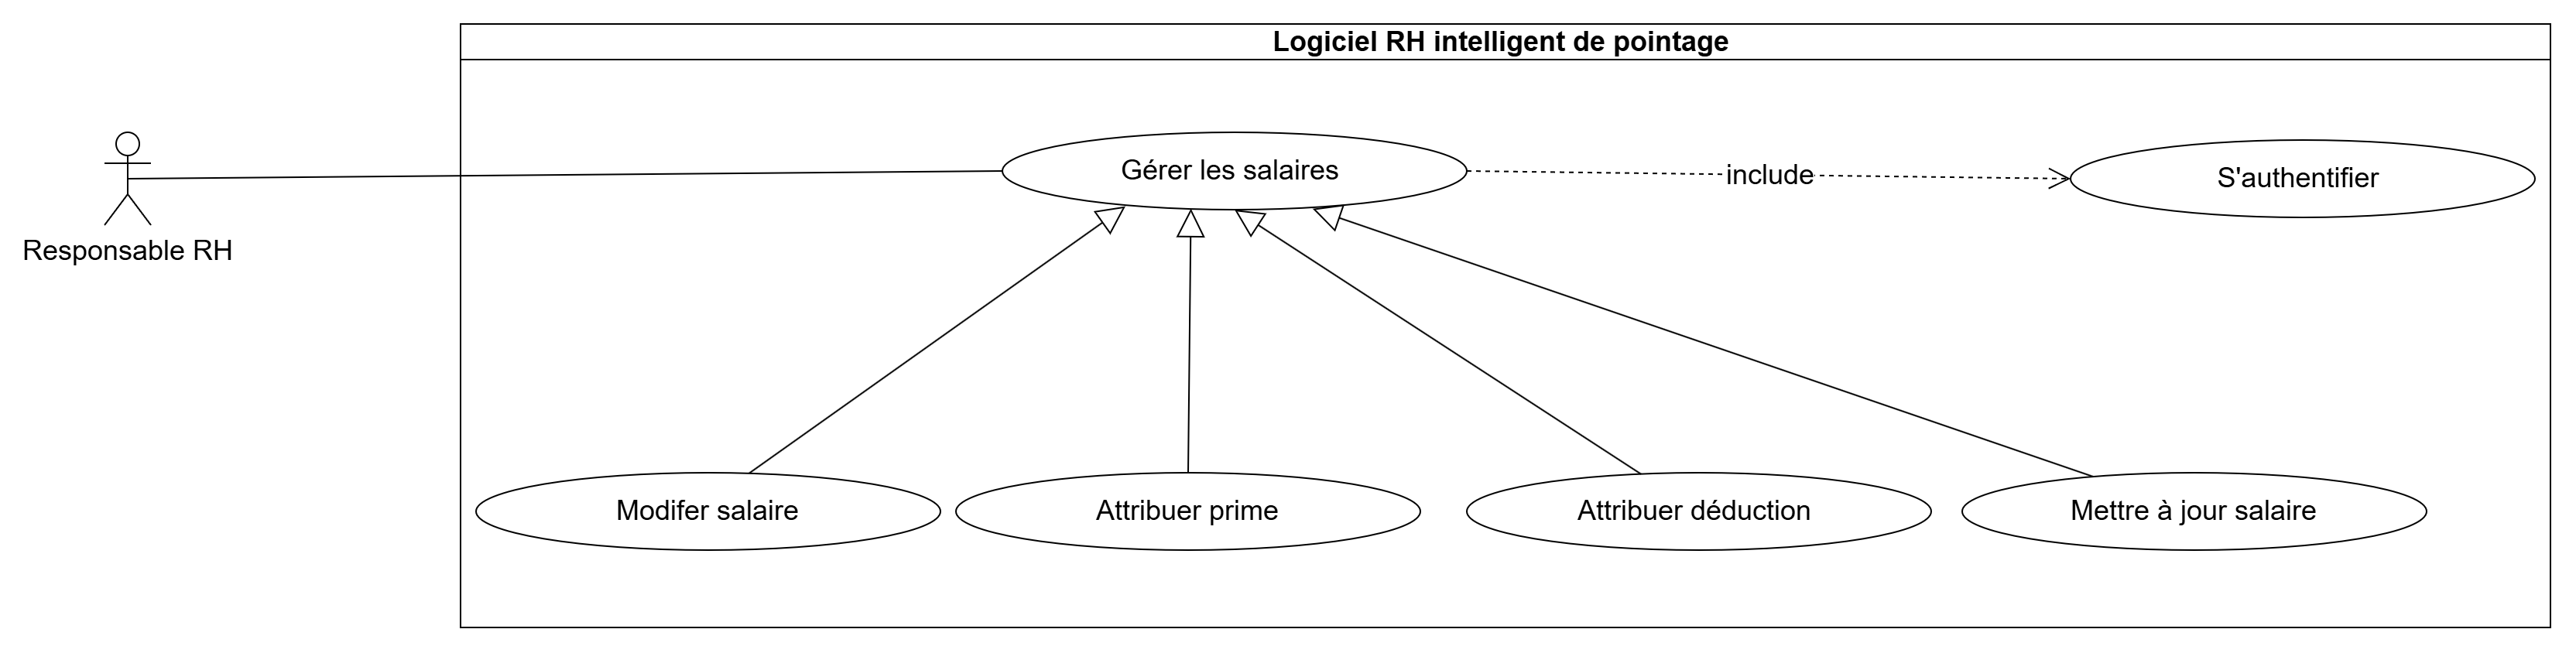
\includegraphics[width=0.9\textwidth]{projet/images/usecase/sprint 3/refinnement_gere_salaire.png}
    \caption{Raffinement du cas d'utilisation "Gérer les salaires"}
    \label{fig:raffinement_gerer_salaires}
\end{figure}

\item \textbf{Description textuelle : cas d'utilisation «~Attribuer déduction~»}

\begin{center}
\begin{longtable}{|p{5cm}|p{11cm}|}
\hline
\textbf{Nom du cas d'utilisation} & Attribuer déduction \\ \hline
\textbf{Acteurs} & Responsable RH \\ \hline
\textbf{Objectif} & Attribuer une déduction à un employé \\ \hline
\textbf{Préconditions} & Responsable RH authentifié \\ \hline
\textbf{Scénario nominal} &
1. Accéder à l'interface de gestion des salaires. \newline
2. Cliquer sur le bouton «~Ajouter une déduction~». \newline
3. Saisir les coordonnées de l'employé (ID ou nom complet). \newline
4. Saisir le montant, le motif et la description de la déduction. \newline
5. Valider l'attribution. \newline
6. Le système enregistre la déduction. \\ \hline
\textbf{Scénario d'exception} & Montant ou raison invalide $\rightarrow$ message d'erreur. \\ \hline
\textbf{Post-condition} & La déduction est attribuée et visible pour l'employé. \\ \hline
\caption{Description textuelle du cas d'utilisation «~Attribuer déduction~»}
\end{longtable}
\end{center}

\item \textbf{Description textuelle : cas d'utilisation «~Attribuer prime~»}

\begin{center}
\begin{longtable}{|p{5cm}|p{11cm}|}
\hline
\textbf{Nom du cas d'utilisation} & Attribuer prime \\ \hline
\textbf{Acteurs} & Responsable RH \\ \hline
\textbf{Objectif} & Attribuer une prime à un employé \\ \hline
\textbf{Préconditions} & Responsable RH authentifié \\ \hline
\textbf{Scénario nominal} &
1. Accéder à l'interface de gestion des salaires. \newline
2. Cliquer sur le bouton «~Ajouter une prime~». \newline
3. Saisir les coordonnées de l'employé (ID ou nom complet). \newline
4. Saisir le montant, le motif et la description de la prime. \newline
5. Valider l'attribution. \newline
6. Le système enregistre la prime. \\ \hline
\textbf{Scénario d'exception} & Montant ou raison invalide $\rightarrow$ message d'erreur. \\ \hline
\textbf{Post-condition} & La prime est attribuée et visible pour l'employé. \\ \hline
\caption{Description textuelle du cas d'utilisation «~Attribuer prime~»}
\end{longtable}
\end{center}



\item \textbf{Description textuelle : cas d'utilisation «~Mettre à jour statut salaire~»}

\begin{center}
\begin{longtable}{|p{5cm}|p{11cm}|}
\hline
\textbf{Nom du cas d'utilisation} & Mettre à jour statut salaire \\ \hline
\textbf{Acteurs} & Responsable RH \\ \hline
\textbf{Objectif} & Mettre à jour le statut du salaire \\ \hline
\textbf{Préconditions} & Responsable RH authentifié \\ \hline
\textbf{Scénario nominal} &
1. Accéder à l'interface de Gestion Salaires. \newline
2. Sélectionner l'employé. \newline
3. Mettre à jour le statut (En Attente / Payé / Traité). \newline
4. Valider la modification. \newline
5. Le système enregistre le nouveau statut. \\ \hline
\textbf{Scénario d'exception} & Informations manquantes $\rightarrow$ message d'erreur. \\ \hline
\textbf{Post-condition} & Le statut du salaire est mis à jour. \\ \hline
\caption{Description textuelle du cas d'utilisation «~Mettre à jour statut salaire~»}
\end{longtable}
\end{center}

\item \textbf{Description textuelle : cas d'utilisation «~Modifier salaire~»}

\begin{center}
\begin{longtable}{|p{5cm}|p{11cm}|}
\hline
\textbf{Nom du cas d'utilisation} & Modifier salaire \\ \hline
\textbf{Acteurs} & Responsable RH \\ \hline
\textbf{Objectif} & Modifier un salaire de base à un employé \\ \hline
\textbf{Préconditions} & Responsable RH authentifié \\ \hline
\textbf{Scénario nominal} &
1. Accéder à l'interface de Gestion Salaires. \newline
2. Sélectionner l'employé. \newline
3. Cliquer sur le bouton modifier. \newline
4. Mettre à jour le salaire. \newline
5. Valider la modification. \newline
6. Le système enregistre le nouveau salaire. \\ \hline
\textbf{Scénario d'exception} & Salaire invalide $\rightarrow$ message d'erreur. \\ \hline
\textbf{Post-condition} & Le salaire est mis à jour. \\ \hline
\caption{Description textuelle du cas d'utilisation «~Modifier salaire~»}
\end{longtable}
\end{center}

\item \textbf{Raffinement du cas d'utilisation "Gérer documents"}

\begin{figure}[H]
    \centering
    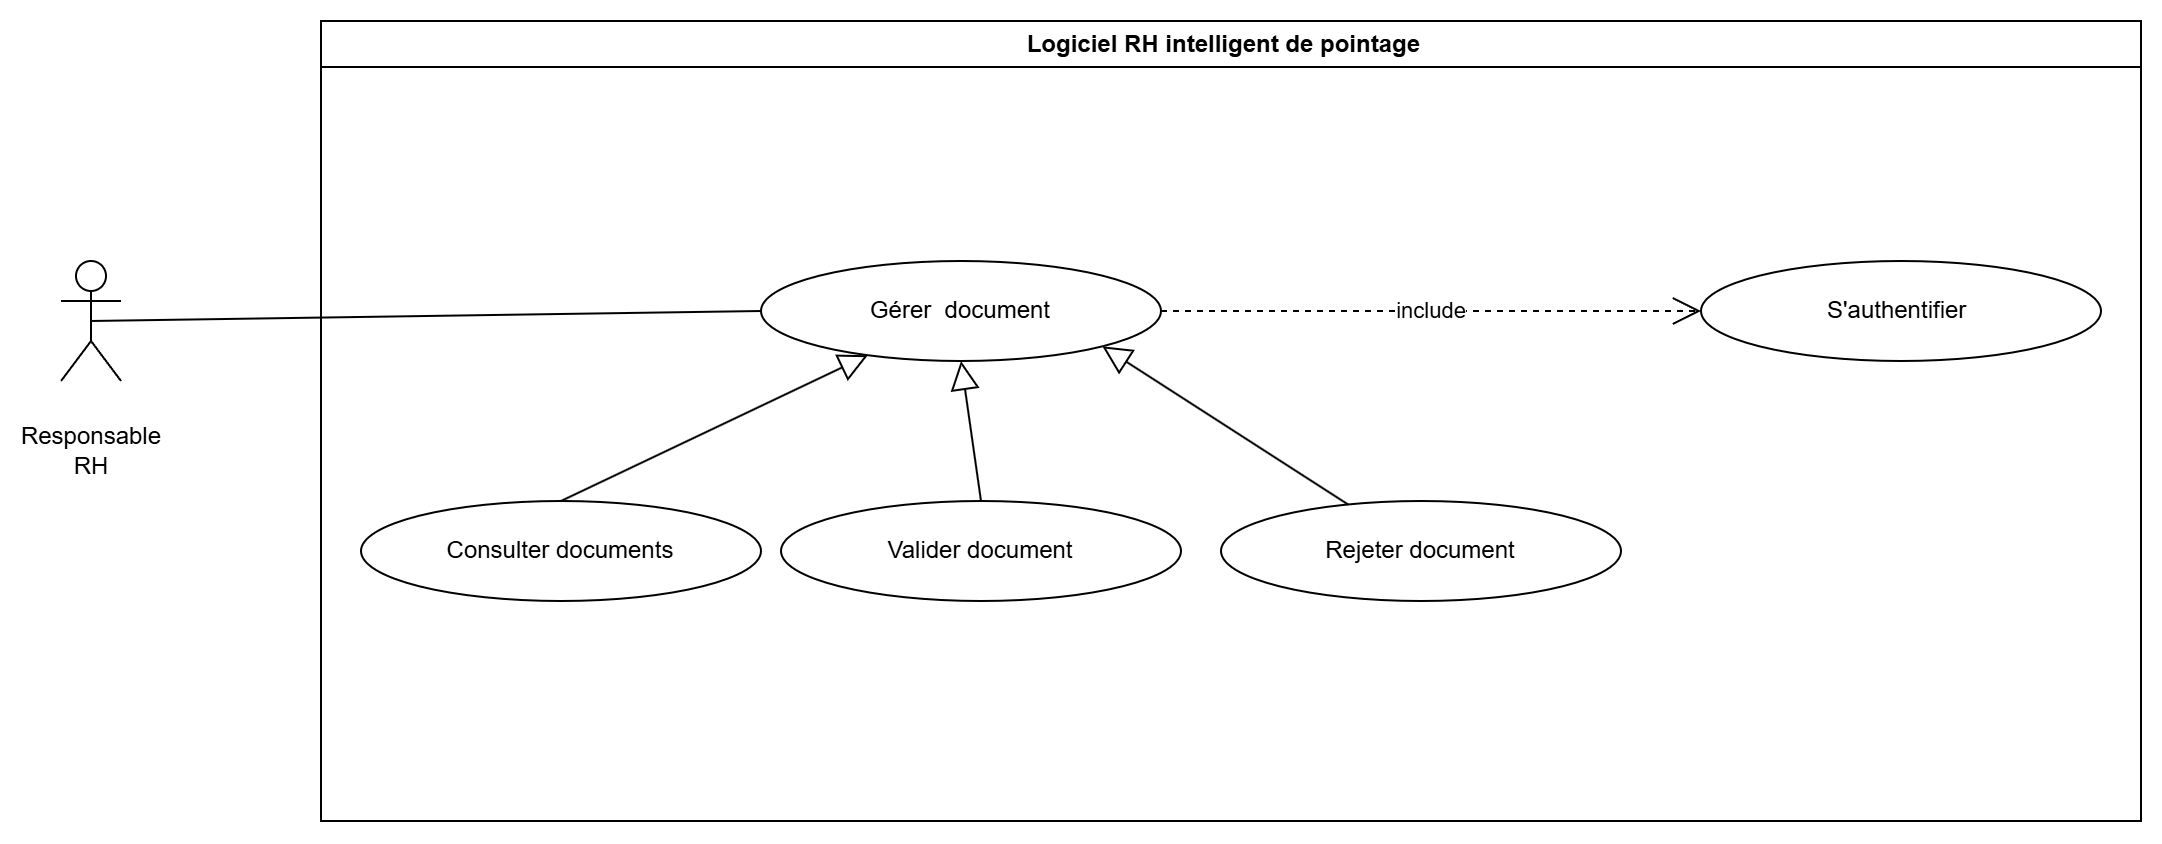
\includegraphics[width=0.9\textwidth]{projet/images/usecase/sprint 3/gerer_document.png}
    \caption{Raffinement du cas d'utilisation "Gérer documents"}
    \label{fig:raffinement_gerer_documents}
\end{figure}

\item \textbf{Description textuelle : cas d'utilisation «~Consulter documents~»}

\begin{center}
\begin{longtable}{|p{5cm}|p{11cm}|}
\hline
\textbf{Nom du cas d'utilisation} & Consulter documents \\ \hline
\textbf{Acteurs} & Responsable RH \\ \hline
\textbf{Objectif} & Consulter les documents envoyés \\ \hline
\textbf{Préconditions} & Responsable RH authentifié \\ \hline
\textbf{Scénario nominal} &
1. Accéder à l'interface des documents. \newline
2. Sélectionner un document. \newline
3. Afficher les détails du document. \\ \hline
\textbf{Scénario d'exception} & Document manquant $\rightarrow$ message "Document non disponible". \\ \hline
\textbf{Post-condition} & Les documents sont consultés. \\ \hline
\caption{Description textuelle du cas d'utilisation «~Consulter documents~»}
\end{longtable}
\end{center}

\item \textbf{Description textuelle : cas d'utilisation «~Valider document~»}

\begin{center}
\begin{longtable}{|p{5cm}|p{11cm}|}
\hline
\textbf{Nom du cas d'utilisation} & Valider document \\ \hline
\textbf{Acteurs} & Responsable RH \\ \hline
\textbf{Objectif} & Approuver un document \\ \hline
\textbf{Préconditions} & Responsable RH authentifié \\ \hline
\textbf{Scénario nominal} &
1. Accéder aux documents. \newline
2. Sélectionner un document. \newline
3. Cliquer sur "Valider". \newline
4. Le système met à jour le statut du document. \\ \hline
\textbf{Scénario d'exception} & Document inexistant $\rightarrow$ message d'erreur. \\ \hline
\textbf{Post-condition} & Document validé. \\ \hline
\caption{Description textuelle du cas d'utilisation «~Valider document~»}
\end{longtable}
\end{center}

\item \textbf{Description textuelle : cas d'utilisation «~Rejeter document~»}

\begin{center}
\begin{longtable}{|p{5cm}|p{11cm}|}
\hline
\textbf{Nom du cas d'utilisation} & Rejeter document \\ \hline
\textbf{Acteurs} & Responsable RH \\ \hline
\textbf{Objectif} & Refuser un document \\ \hline
\textbf{Préconditions} & Responsable RH authentifié \\ \hline
\textbf{Scénario nominal} &
1. Accéder aux documents. \newline
2. Sélectionner un document. \newline
3. Cliquer sur "Rejeter". \newline
4. Le système met à jour le statut. \\ \hline
\textbf{Scénario d'exception} & Document inexistant $\rightarrow$ message d'erreur. \\ \hline
\textbf{Post-condition} & Document rejeté. \\ \hline
\caption{Description textuelle du cas d'utilisation «~Rejeter document~»}
\end{longtable}
\end{center}

\item \textbf{Raffinement du cas d'utilisation "Consulter  son salaire"}

\begin{figure}[H]
    \centering
    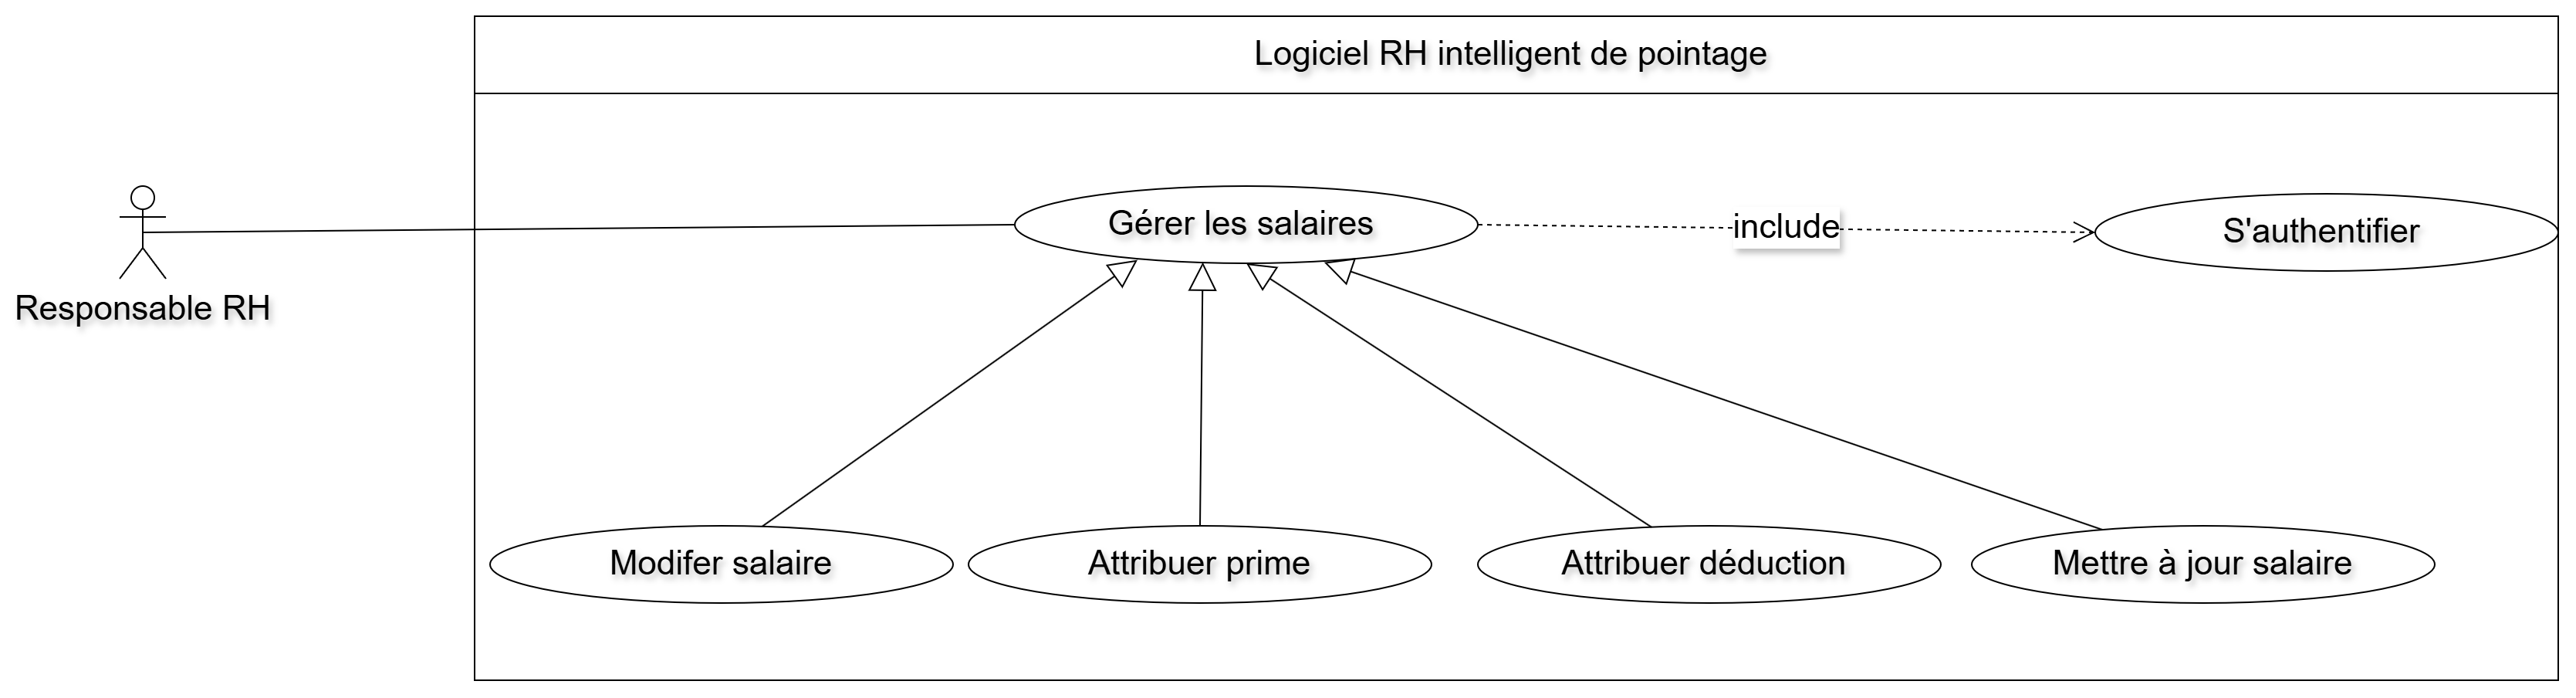
\includegraphics[width=0.9\textwidth]{projet/images/usecase/sprint 3/CS.png}
    \caption{Raffinement du cas d'utilisation "Gérer les salaires"}
    \label{fig:raffinement_gerer_salaires}
\end{figure}
\item \textbf{Description textuelle : cas d'utilisation «~Consulter primes~»}

\begin{center}
\begin{longtable}{|p{5cm}|p{11cm}|}
\hline
\textbf{Nom du cas d'utilisation} & Consulter primes \\ \hline
\textbf{Acteurs} & Employé \\ \hline
\textbf{Objectif} & Consulter mes primes \\ \hline
\textbf{Préconditions} & Employé authentifié \\ \hline
\textbf{Scénario nominal} &
1. Accéder à l'interface de Mon Salaire. \newline
2. Cliquer sur "Cliquer pour consulter primes". \newline
3. Affichage des primes et montants. \\ \hline
\textbf{Scénario d'exception} & Aucune prime $\rightarrow$ message "Aucune prime disponible". \\ \hline
\textbf{Post-condition} & L'employé visualise ses primes. \\ \hline
\caption{Description textuelle du cas d'utilisation «~Consulter primes~»}
\end{longtable}
\end{center}

\item \textbf{Description textuelle : cas d'utilisation «~Consulter déductions~»}

\begin{center}
\begin{longtable}{|p{5cm}|p{11cm}|}
\hline
\textbf{Nom du cas d'utilisation} & Consulter déductions \\ \hline
\textbf{Acteurs} & Employé \\ \hline
\textbf{Objectif} & Consulter mes déductions \\ \hline
\textbf{Préconditions} & Employé authentifié \\ \hline
\textbf{Scénario nominal} &
1. Accéder à l'interface de Mon Salaire. \newline
2. Cliquer sur "Cliquer pour consulter déductions". \newline
3. Affichage des déductions et montants. \\ \hline
\textbf{Scénario d'exception} & Aucune déduction $\rightarrow$ message "Aucune déduction disponible". \\ \hline
\textbf{Post-condition} & L'employé visualise ses déductions. \\ \hline
\caption{Description textuelle du cas d'utilisation «~Consulter déductions~»}
\end{longtable}
\end{center}

\item \textbf{Description textuelle : cas d'utilisation «~Consulter salaire~»}

\begin{center}
\begin{longtable}{|p{5cm}|p{11cm}|}
\hline
\textbf{Nom du cas d'utilisation} & Consulter statut du salaire \\ \hline
\textbf{Acteurs} & Employé \\ \hline
\textbf{Objectif} & Voir le statut du salaire \\ \hline
\textbf{Préconditions} & Employé authentifié \\ \hline
\textbf{Scénario nominal} &
1. Accéder à l'interface de Mon Salaire. \newline
2. Voir Historique des Paiements. \newline
3. Affichage du statut (versé ou non). \\ \hline
\textbf{Scénario d'exception} & Informations manquantes $\rightarrow$ message "Information non disponible". \\ \hline
\textbf{Post-condition} & L'employé connaît le statut de son salaire. \\ \hline
\caption{Description textuelle du cas d'utilisation «~Consulter statut du salaire~»}
\end{longtable}
\end{center}

\item \textbf{Description textuelle : cas d'utilisation «~Demander un congé~»}

\begin{center}
\begin{longtable}{|p{5cm}|p{11cm}|}
\hline
\textbf{Nom du cas d'utilisation} & Demander un congé \\ \hline
\textbf{Acteurs} & Employé \\ \hline
\textbf{Objectif} & Envoyer une demande de congé \\ \hline
\textbf{Préconditions} & Employé authentifié \\ \hline
\textbf{Scénario nominal} &
1. Accéder à l'interface de demande de congé. \newline
2. Cliquer sur "Demander un congé". \newline
3. Saisir date début, date fin et motif. \newline
4. Valider la demande. \newline
5. Le système enregistre et envoie au RH. \\ \hline
\textbf{Scénario d'exception} & Champs vides ou dates incorrectes $\rightarrow$ message d'erreur. \\ \hline
\textbf{Post-condition} & Demande enregistrée et en attente de validation. \\ \hline
\caption{Description textuelle du cas d'utilisation «~Demander un congé~»}
\end{longtable}
\end{center}

\item \textbf{Description textuelle : cas d'utilisation «~Déposer document~»}

\begin{center}
\begin{longtable}{|p{5cm}|p{11cm}|}
\hline
\textbf{Nom du cas d'utilisation} & Déposer document \\ \hline
\textbf{Acteurs} & Employé \\ \hline
\textbf{Objectif} & Déposer un document \\ \hline
\textbf{Préconditions} & Employé authentifié \\ \hline
\textbf{Scénario nominal} &
1. Accéder à l'espace personnel. \newline
2. Cliquer sur "Déposer document". \newline
3. Sélectionner le fichier et saisir les infos. \newline
4. Valider l'envoi. \newline
5. Le système enregistre et notifie le RH. \\ \hline
\textbf{Scénario d'exception} & Fichier invalide ou manquant $\rightarrow$ message d'erreur. \\ \hline
\textbf{Post-condition} & Document enregistré et accessible au RH. \\ \hline
\caption{Description textuelle du cas d'utilisation «~Déposer document~»}
\end{longtable}
\end{center}

\end{itemize}

\subsection{Conception}
Cette section présente les différents diagrammes UML réalisés afin de modéliser le fonctionnement du système, notamment les diagrammes de séquence et les diagrammes de classes, permettant de décrire les interactions entre les acteurs ainsi que la structure globale de l'application.

\subsubsection{Diagramme de séquence du sprint 3}

\begin{itemize}

\item[$\bullet$] \textbf{Diagramme de séquence du cas d'utilisation «~Valider congé~»}

Ce diagramme illustre la validation d'une demande de congé par le Responsable RH. Il consulte la liste des demandes en attente, sélectionne celle à traiter et le système met à jour son statut en approuvé et notifie l'employé concerné.

\begin{figure}[H]
    \centering
    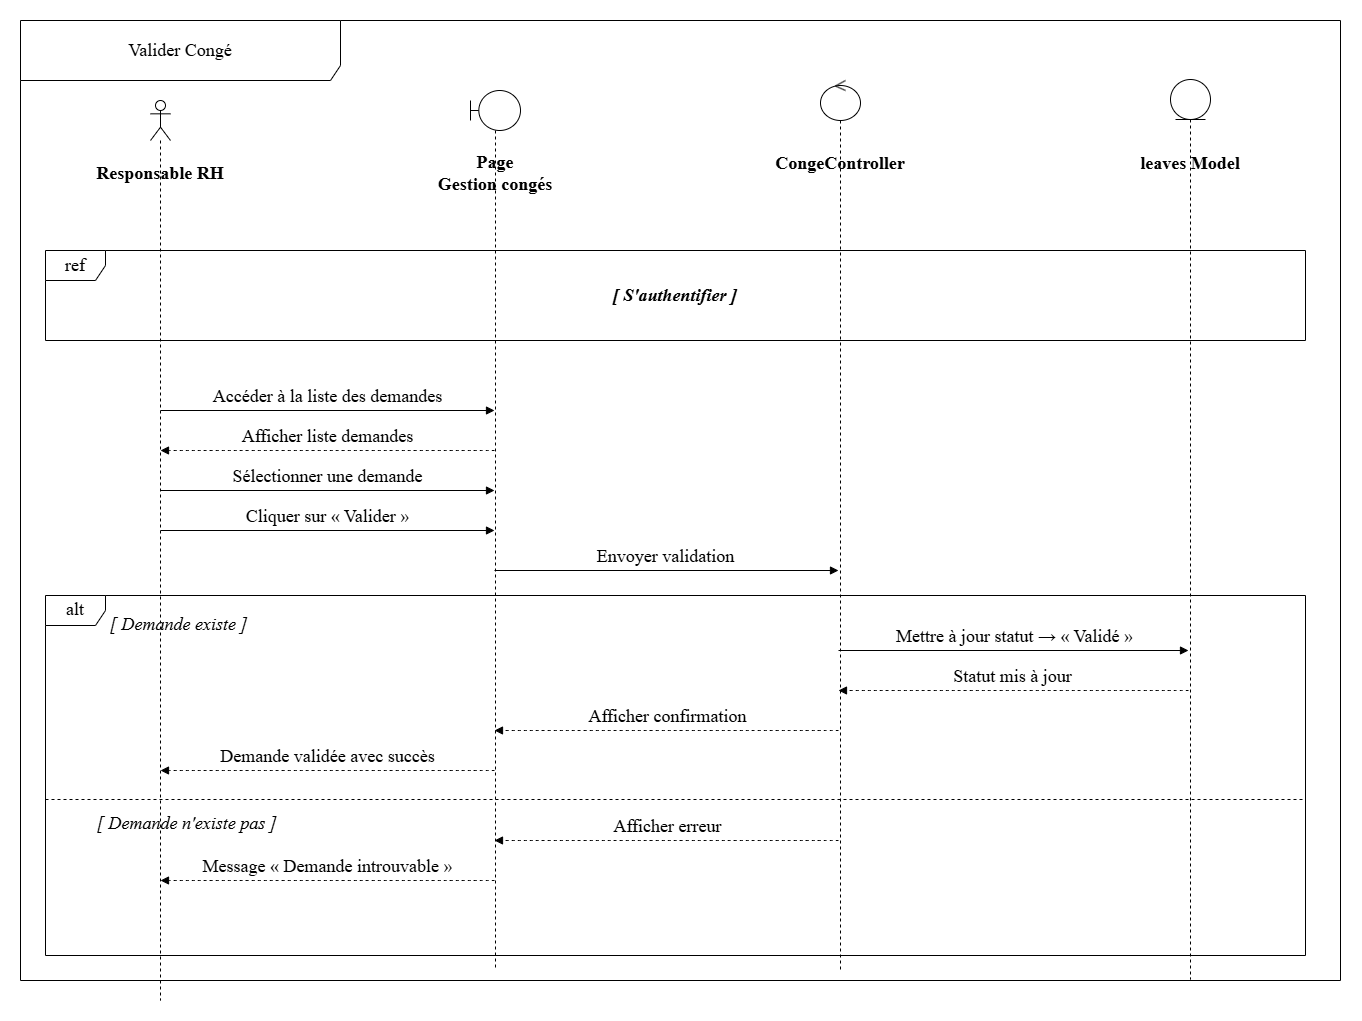
\includegraphics[width=0.9\textwidth]{projet/images/sequence s3/valider conger.drawio.png}
    \caption{Diagramme de séquence du cas d'utilisation «~Valider congé~»}
\end{figure}

\item[$\bullet$] \textbf{Diagramme de séquence du cas d'utilisation «~Refuser congé~»}

Ce diagramme décrit le refus d'une demande de congé par le Responsable RH. Après sélection de la demande, il saisit un motif de refus obligatoire et le système met à jour le statut en refusé avant de notifier l'employé.

\begin{figure}[H]
    \centering
    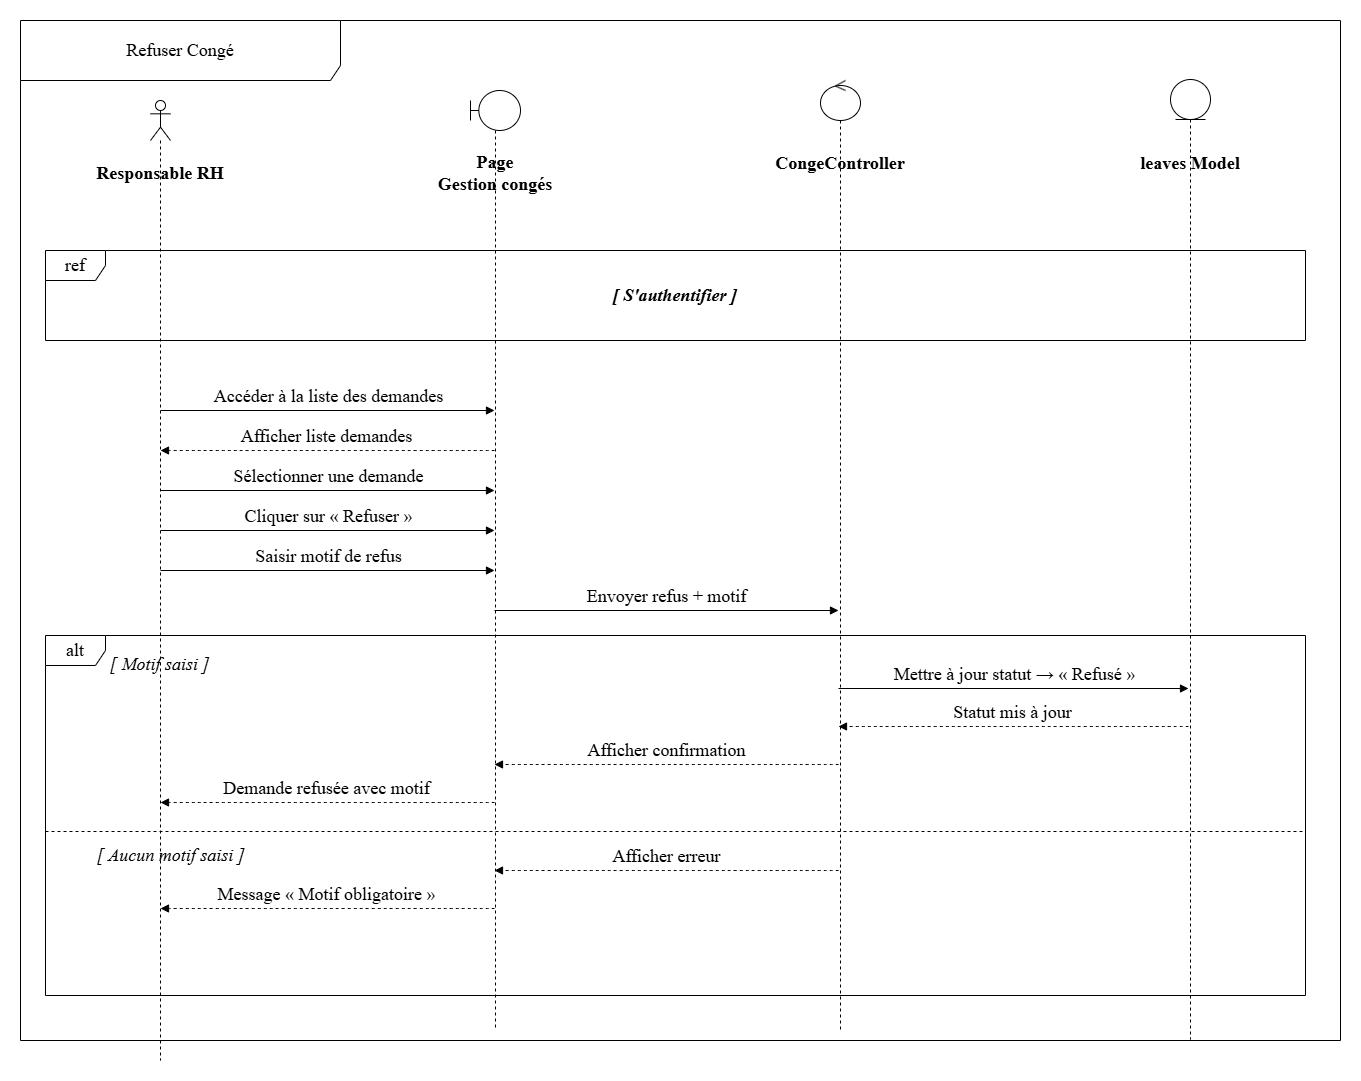
\includegraphics[width=0.9\textwidth]{projet/images/sequence s3/refuser conges.drawio.png}
    \caption{Diagramme de séquence du cas d'utilisation «~Refuser congé~»}
\end{figure}

\item[$\bullet$] \textbf{Diagramme de séquence du cas d'utilisation «~Attribuer prime~»}

Ce diagramme présente l'attribution d'une prime à un employé par le Responsable RH. Il sélectionne l'employé, saisit le montant et la raison de la prime, et le système enregistre l'opération qui devient alors consultable par l'employé concerné.

\begin{figure}[H]
    \centering
    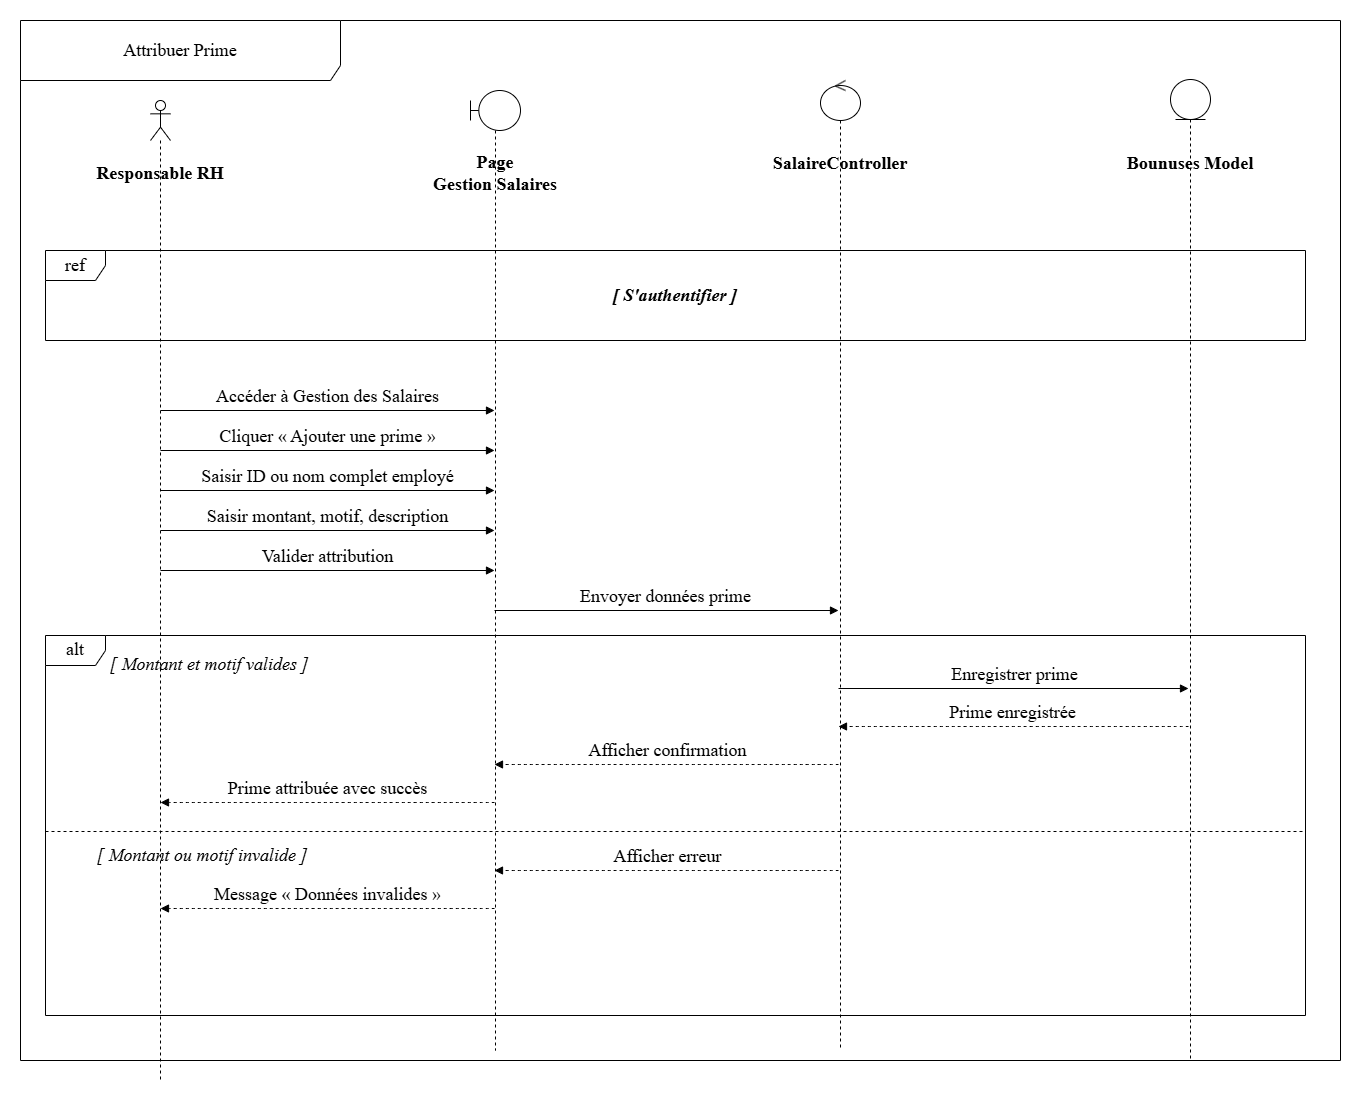
\includegraphics[width=0.9\textwidth]{projet/images/sequence s3/attribuer bounuses.drawio.png}
    \caption{Diagramme de séquence du cas d'utilisation «~Attribuer prime~»}
\end{figure}

\item[$\bullet$] \textbf{Diagramme de séquence du cas d'utilisation «~Attribuer déduction~»}

Ce diagramme illustre l'application d'une déduction sur le salaire d'un employé par le Responsable RH. Il sélectionne l'employé, saisit le montant et le motif de la déduction, et le système enregistre l'opération pour qu'elle soit reflétée dans la fiche de paie.

\begin{figure}[H]
    \centering
    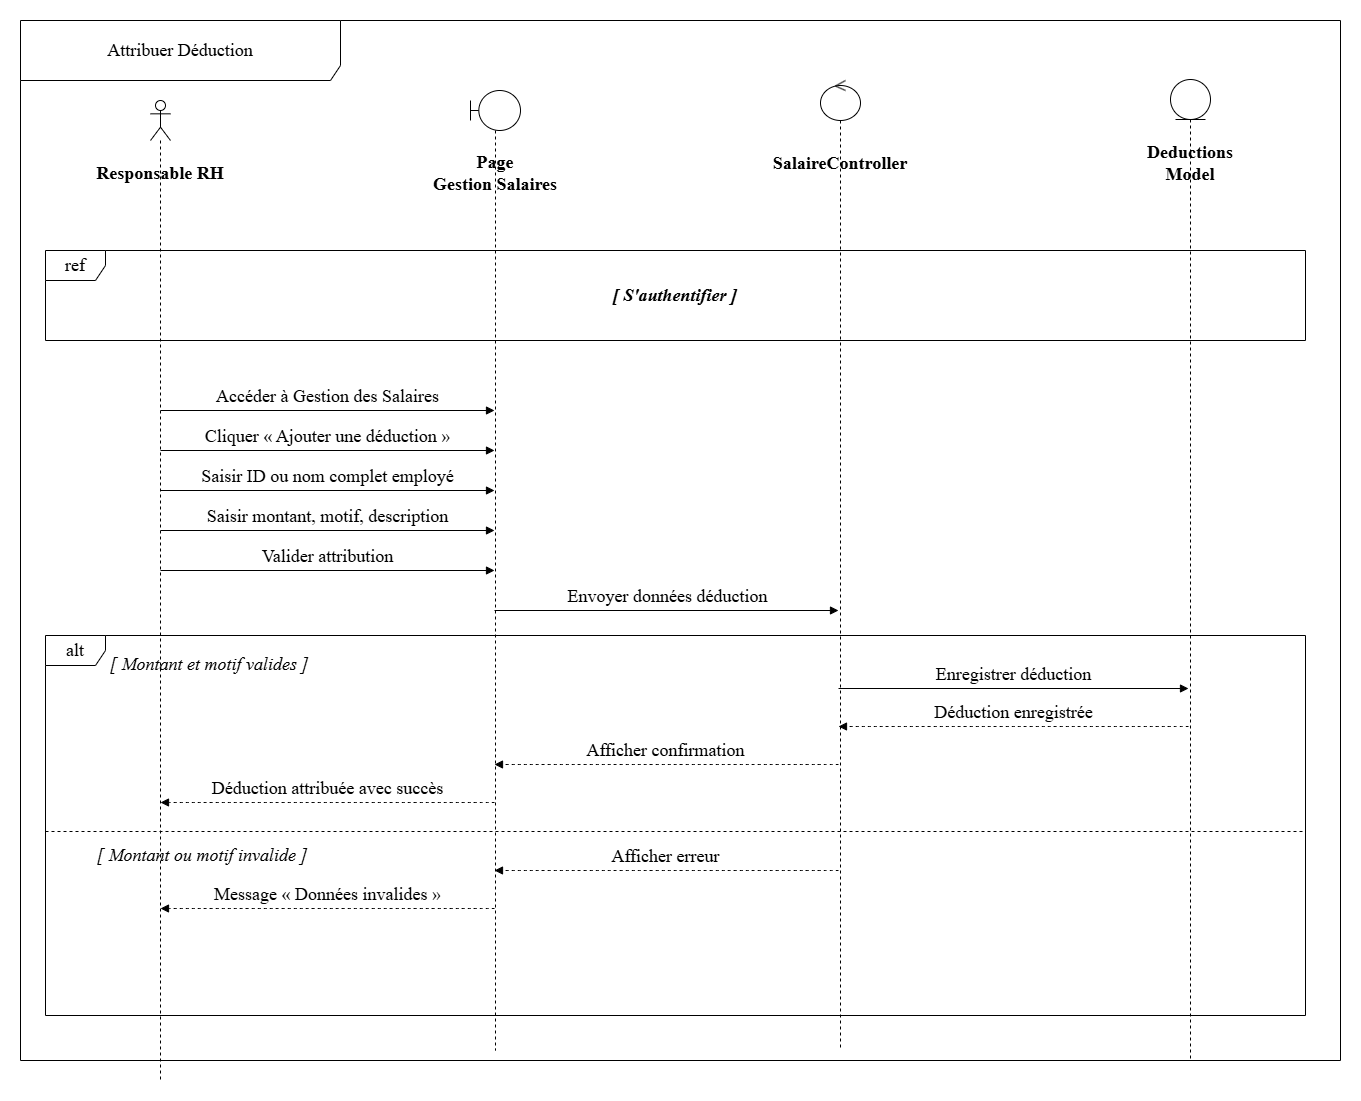
\includegraphics[width=0.9\textwidth]{projet/images/sequence s3/attribuer deduction.drawio.png}
    \caption{Diagramme de séquence du cas d'utilisation «~Attribuer déductions~»}
\end{figure}

\item[$\bullet$] \textbf{Diagramme de séquence du cas d'utilisation «~Mettre à jour statut salaire~»}

Ce diagramme décrit la mise à jour du statut de paiement du salaire d'un employé par le Responsable RH. Il sélectionne l'employé, choisit le nouveau statut (versé ou non versé) et le système enregistre la modification pour la rendre visible à l'employé.

\begin{figure}[H]
    \centering
    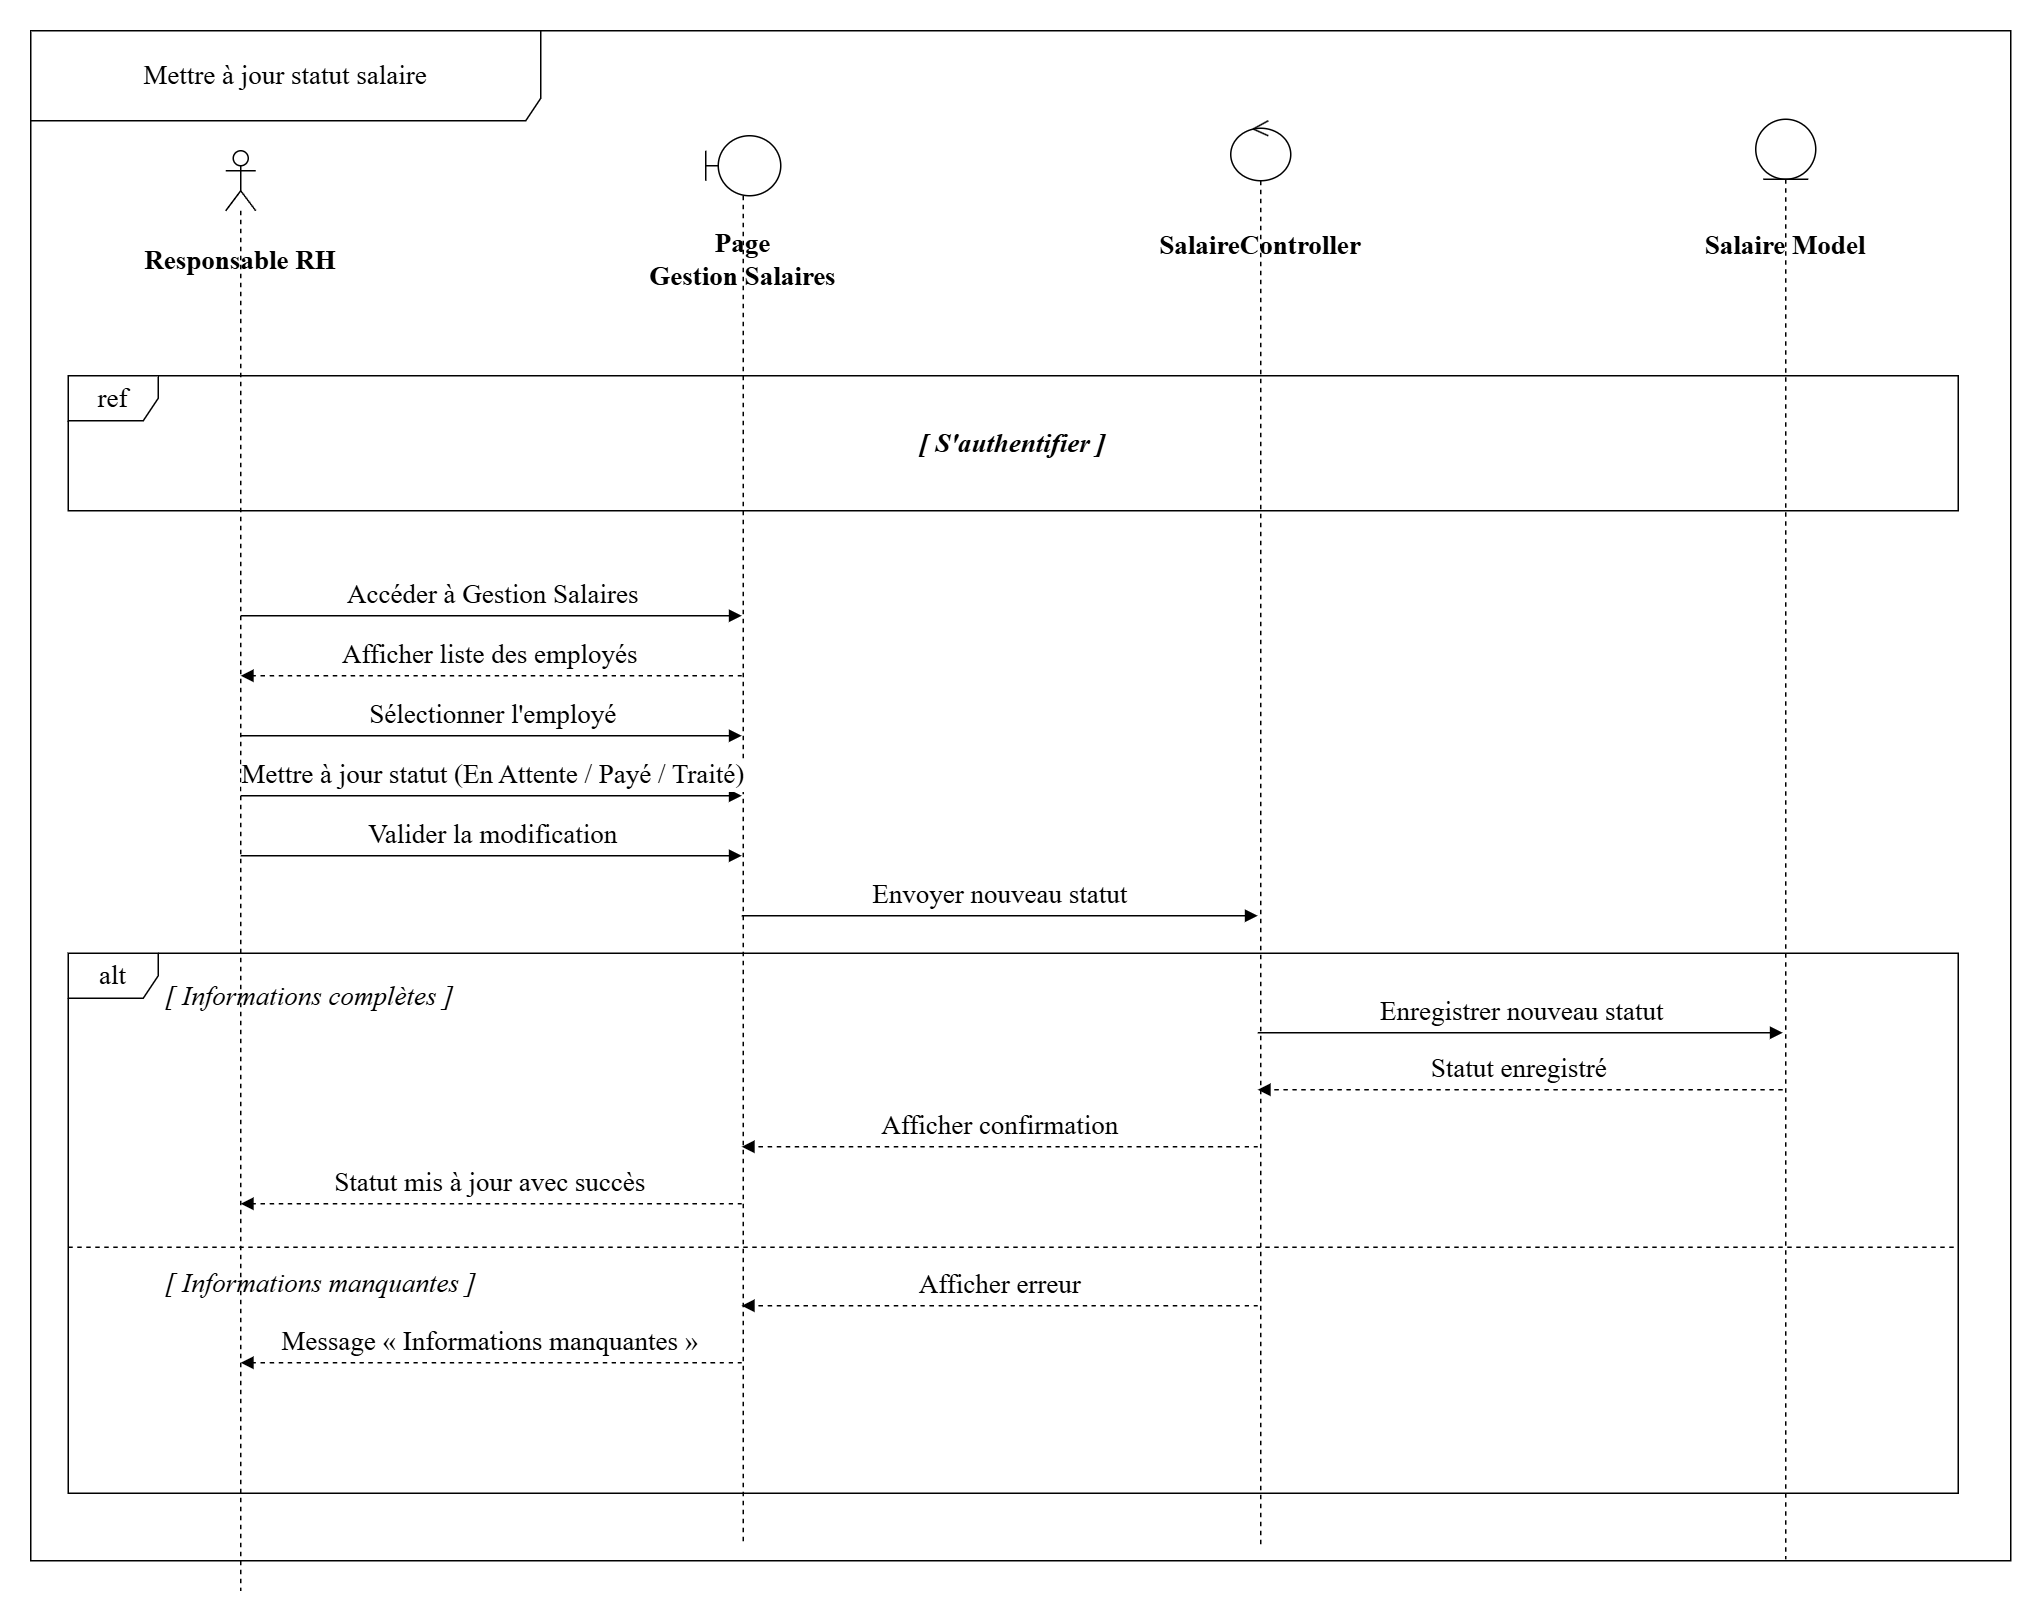
\includegraphics[width=0.9\textwidth]{projet/images/sequence s3/mis_ajour_salaire.png}
    \caption{Diagramme de séquence du cas d'utilisation «~Mettre à jour statut salaire~»}
\end{figure}

\item[$\bullet$] \textbf{Diagramme de séquence du cas d'utilisation «~Modifier salaire~»}

Ce diagramme décrit la mise à jour du statut de paiement du salaire d'un employé par le Responsable RH. Il sélectionne l'employé, choisit le nouveau statut (versé ou non versé) et le système enregistre la modification pour la rendre visible à l'employé.

\begin{figure}[H]
    \centering
    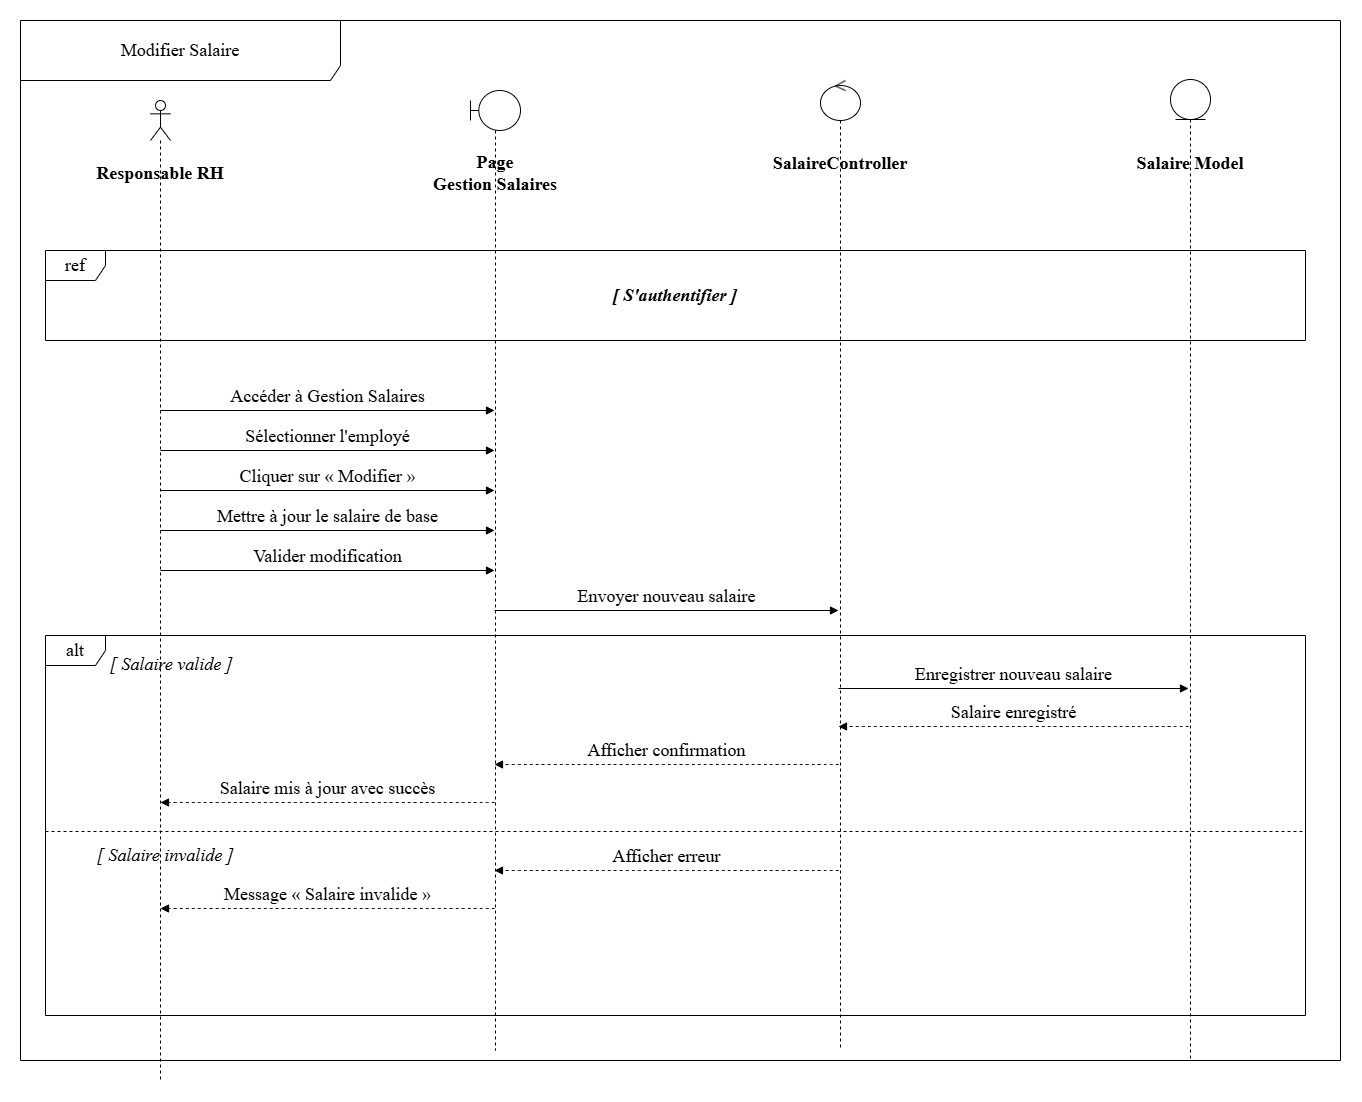
\includegraphics[width=0.9\textwidth]{projet/images/sequence s3/Modifier salaire.drawio.png}
    \caption{Diagramme de séquence du cas d'utilisation «~Modifier salaire~»}
\end{figure}

\item[$\bullet$] \textbf{Diagramme de séquence du cas d'utilisation «~Consulter documents~»}

Ce diagramme présente la consultation des documents soumis par les employés. Le Responsable RH accède à l'interface des documents, sélectionne un document et le système affiche ses détails ou indique son indisponibilité.

\begin{figure}[H]
    \centering
    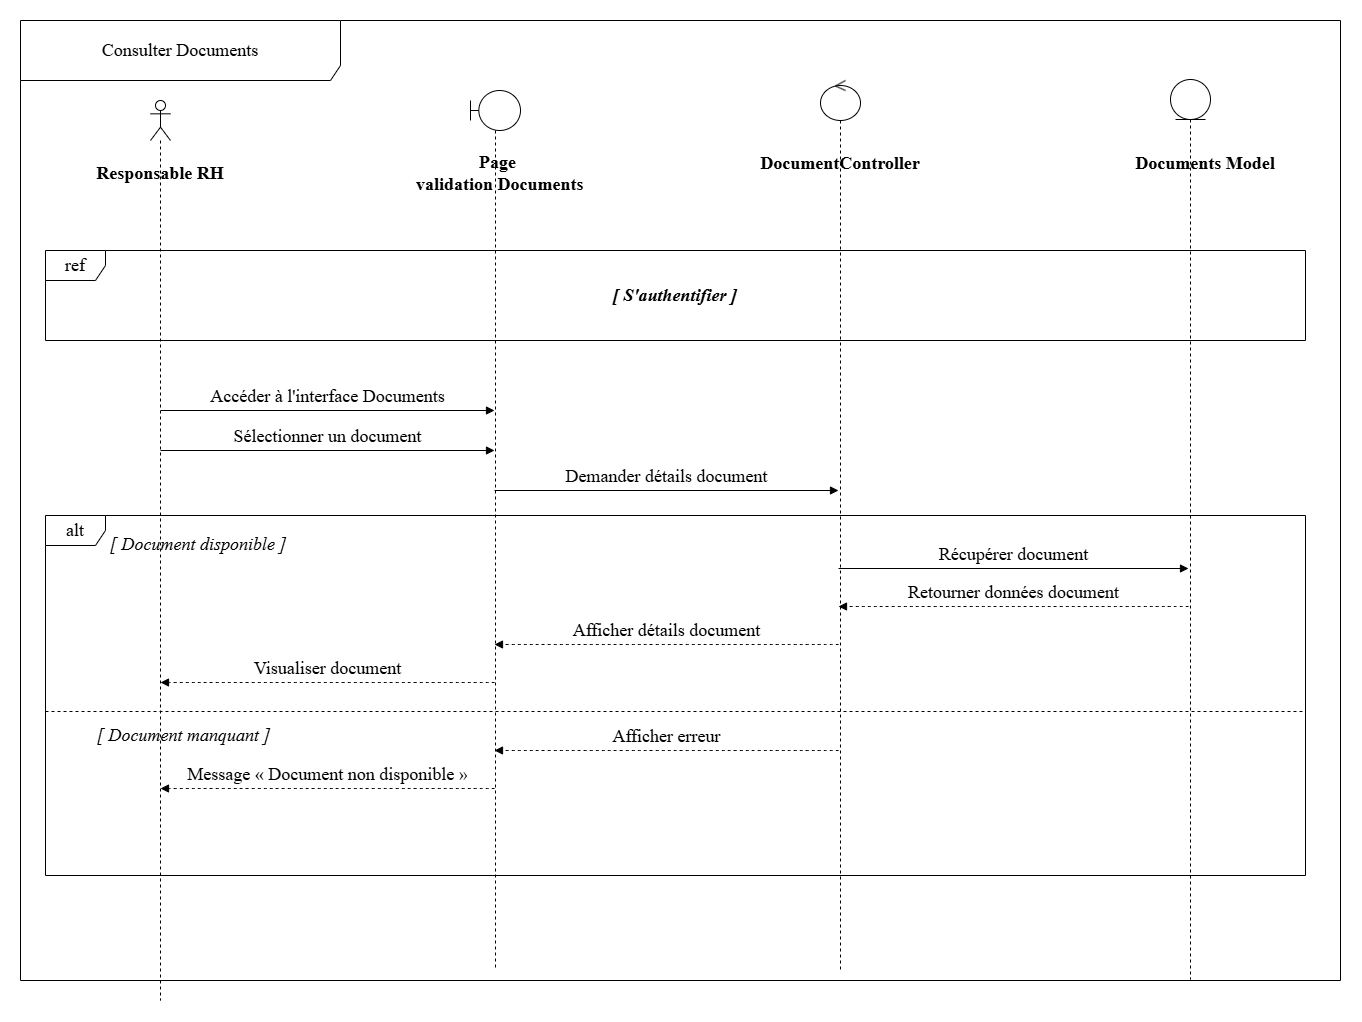
\includegraphics[width=0.9\textwidth]{projet/images/sequence s3/_consulter documents.drawio.png}
    \caption{Diagramme de séquence du cas d'utilisation «~Consulter documents~»}
\end{figure}

\item[$\bullet$] \textbf{Diagramme de séquence du cas d'utilisation «~Valider ou Rejeter document~»}

Ce diagramme illustre la validation ou le rejet d'un document soumis par un employé. Le Responsable RH sélectionne le document, clique sur valider ou rejeter et le système met à jour son statut en approuvé, le rendant officiellement accepté dans le dossier de l'employé.

\begin{figure}[H]
    \centering
    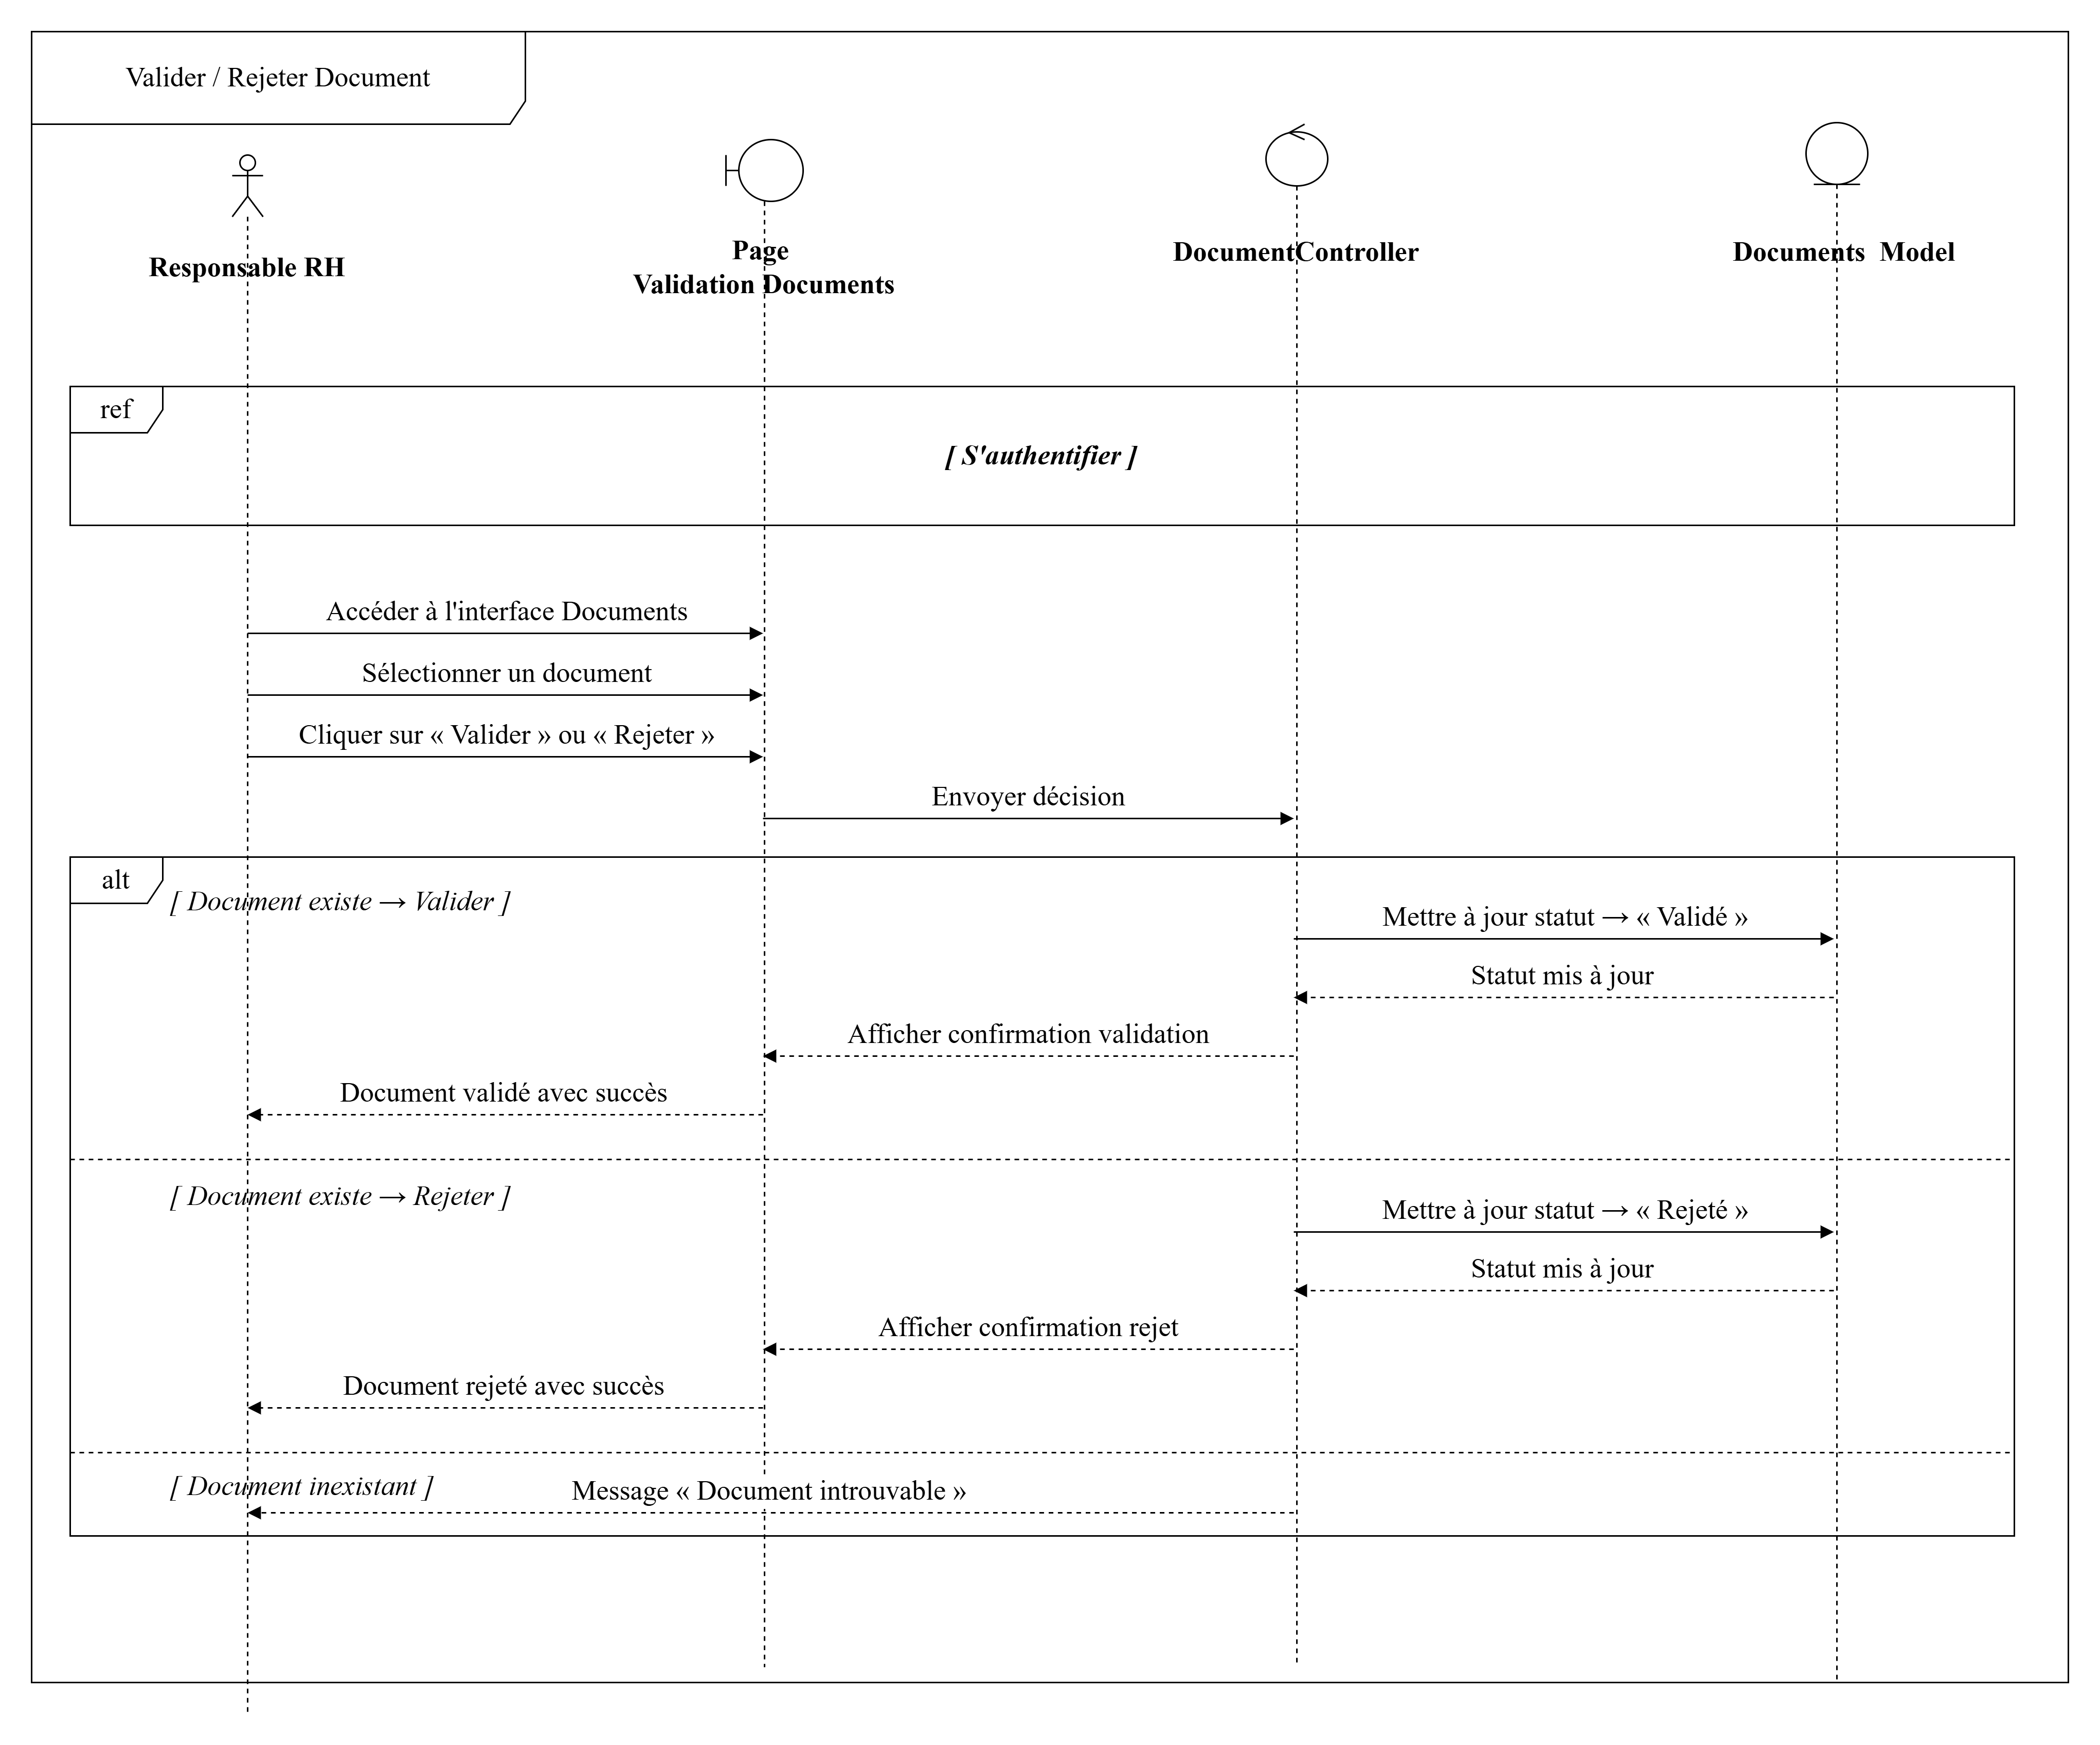
\includegraphics[width=0.9\textwidth]{projet/images/sequence s3/Valider document.drawio.png}
    \caption{Diagramme de séquence du cas d'utilisation «~Valider ou Rejeter document~»}
\end{figure}

\item[$\bullet$] \textbf{Diagramme de séquence du cas d'utilisation «~Consulter prime~»}

Ce diagramme présente la consultation par l'employé de la liste de ses primes attribuées. Il accède à son espace personnel, le système récupère l'historique des primes depuis la base de données et les affiche avec les montants et les dates correspondants.

\begin{figure}[H]
    \centering
    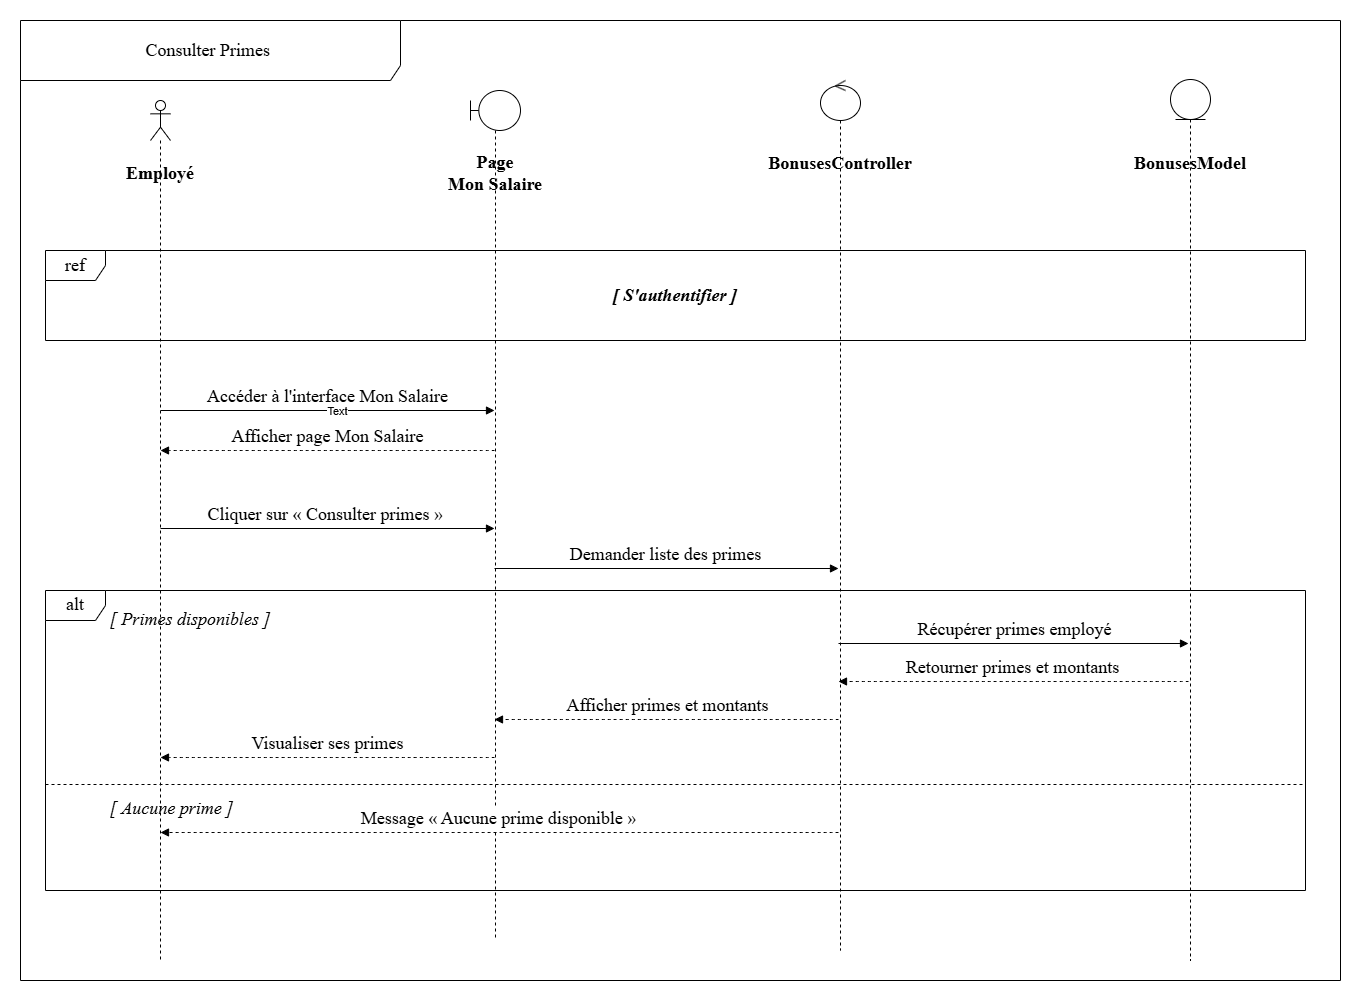
\includegraphics[width=0.9\textwidth]{projet/images/sequence s3/consulter_primes_et_deductions.png}
    \caption{Diagramme de séquence du cas d'utilisation «~Consulter prime~»}
\end{figure}

\item[$\bullet$] \textbf{Diagramme de séquence du cas d'utilisation «~Consulter déduction~»}

Ce diagramme illustre la consultation par l'employé de ses déductions appliquées. Il accède à la section dédiée de son espace personnel, le système récupère les données et les affiche avec les montants et les motifs associés à chaque déduction.

\begin{figure}[H]
    \centering
    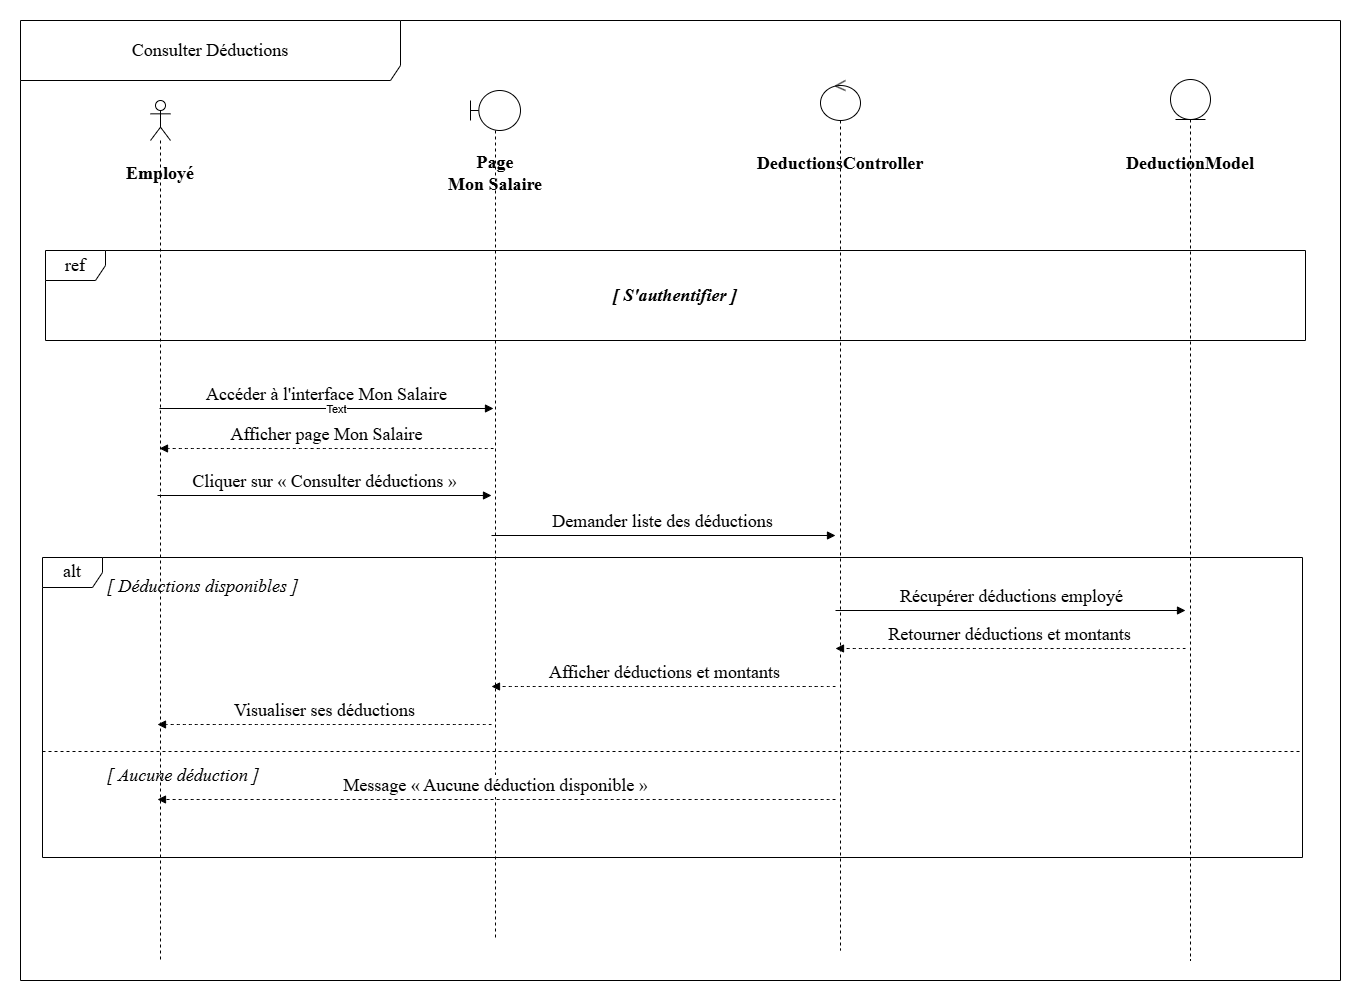
\includegraphics[width=0.9\textwidth]{projet/images/sequence s3/consulter_deductions.png}
    \caption{Diagramme de séquence du cas d'utilisation «~Consulter déduction~»}
\end{figure}

\item[$\bullet$] \textbf{Diagramme de séquence du cas d'utilisation «~Consulter salaire~»}

Ce diagramme décrit la consultation par l'employé du statut de son salaire mensuel. Il accède à son espace personnel, le système interroge la base de données et affiche le statut actuel du salaire, indiquant s'il a été versé ou non.

\begin{figure}[H]
    \centering
    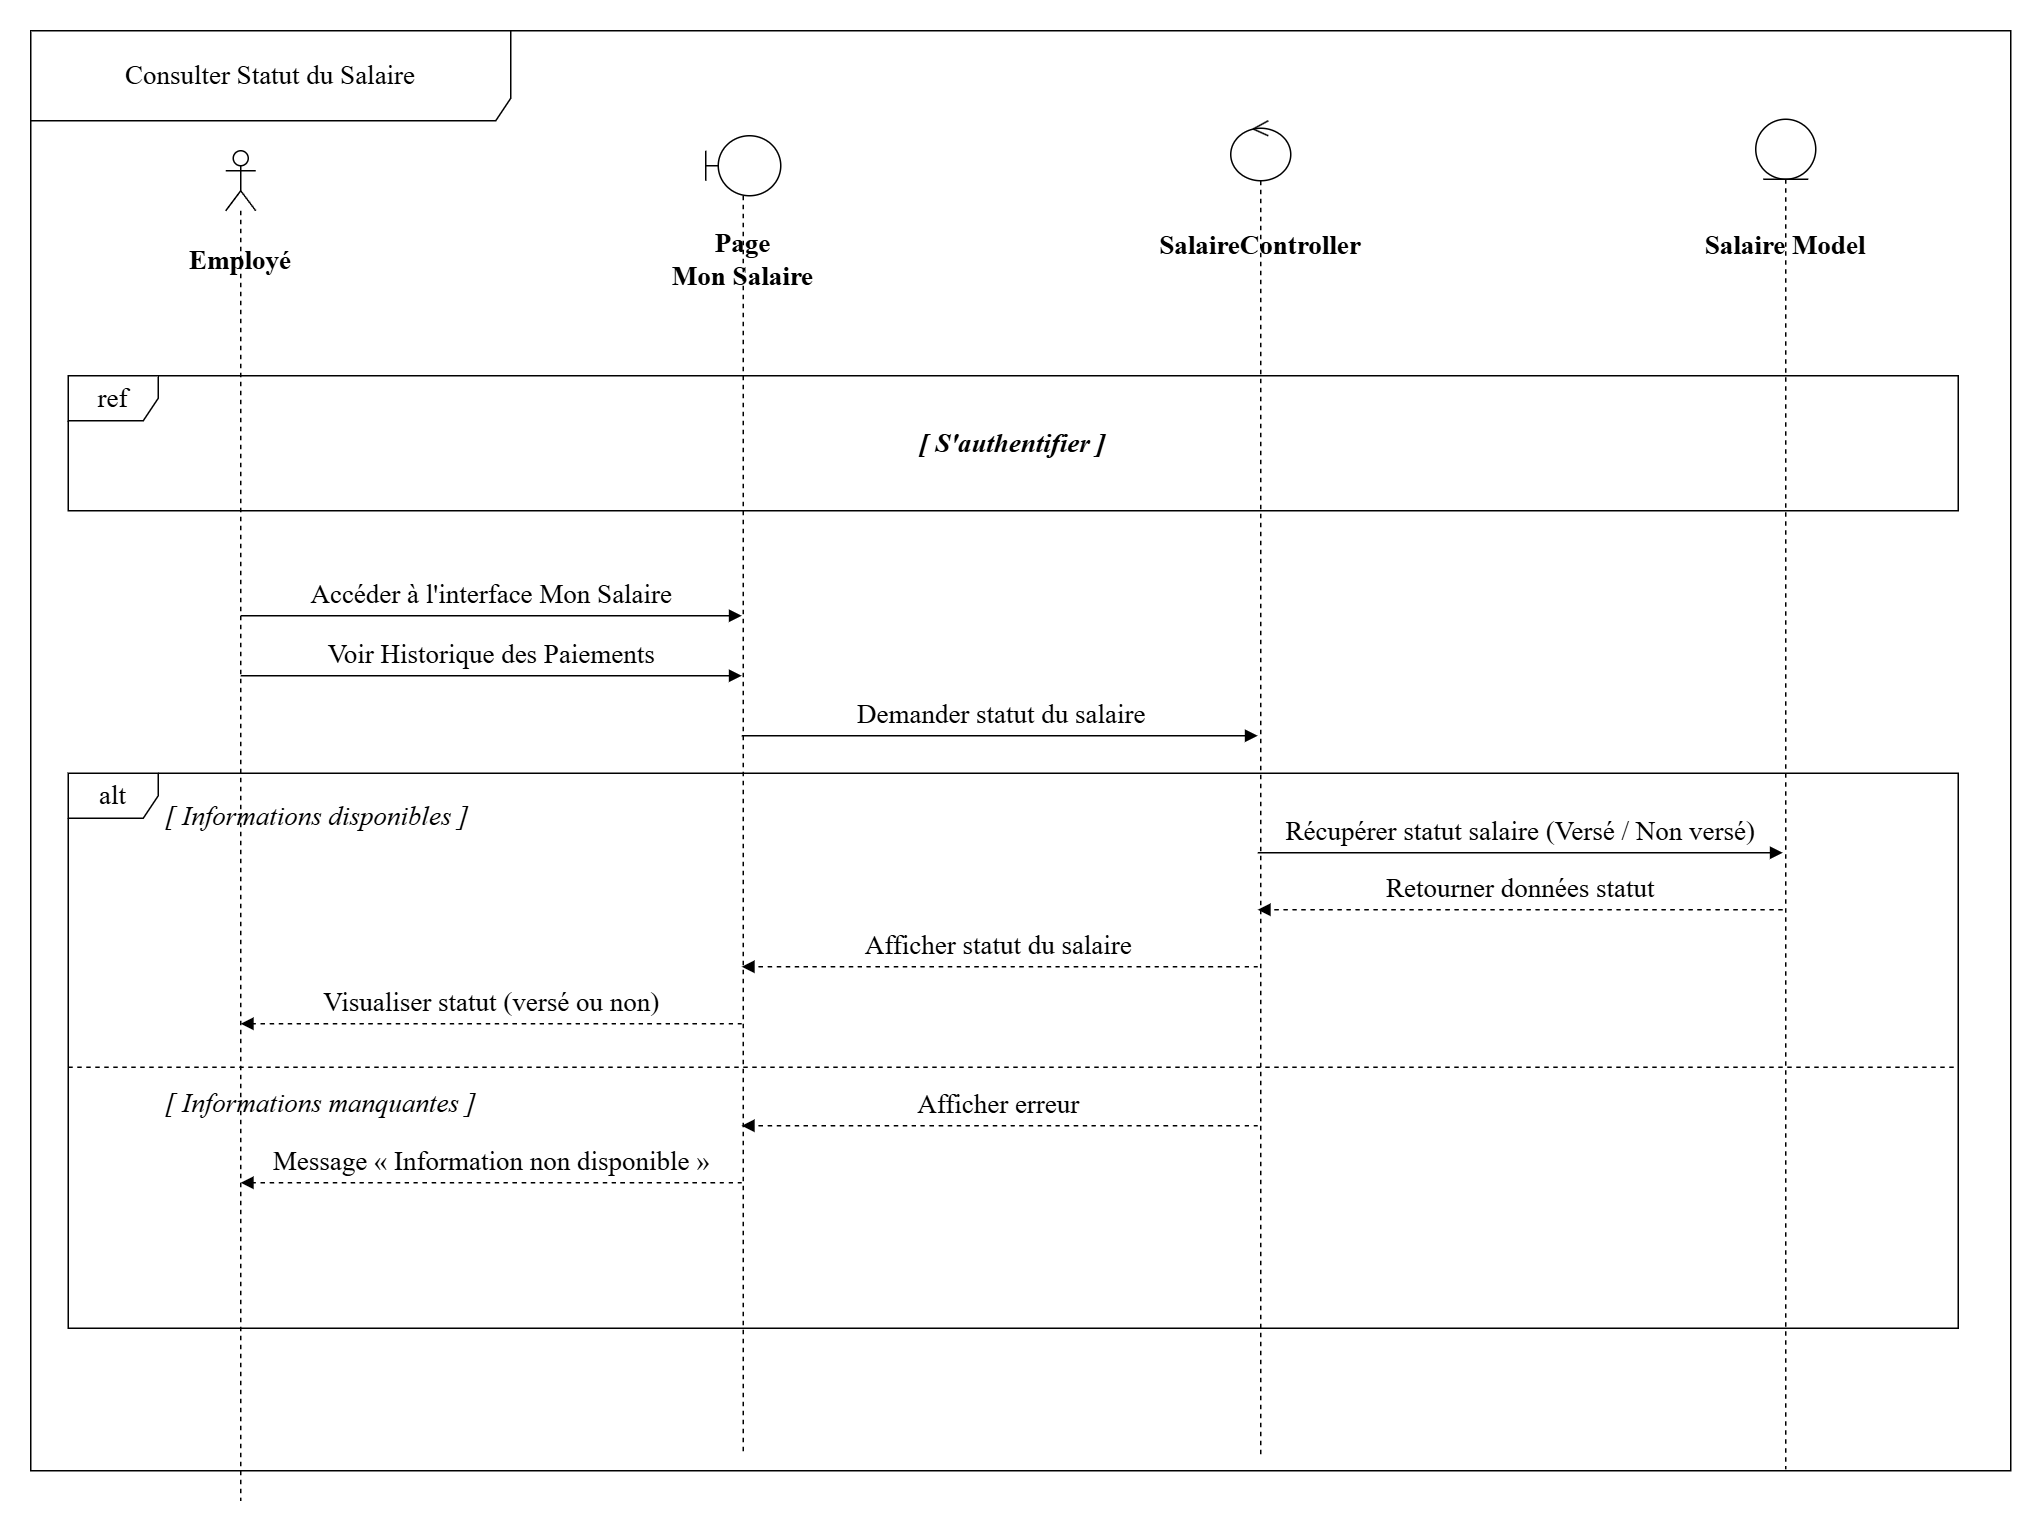
\includegraphics[width=0.9\textwidth]{projet/images/sequence s3/consulter_salaires.png}
    \caption{Diagramme de séquence du cas d'utilisation «~Consulter salaire~»}
\end{figure}

\item[$\bullet$] \textbf{Diagramme de séquence du cas d'utilisation «~Faire une demande de congé~»}

Ce diagramme présente le processus de soumission d'une demande de congé par l'employé. Il saisit les dates de début et de fin ainsi que le motif, le système enregistre la demande et la transmet au Responsable RH pour traitement.

\begin{figure}[H]
    \centering
    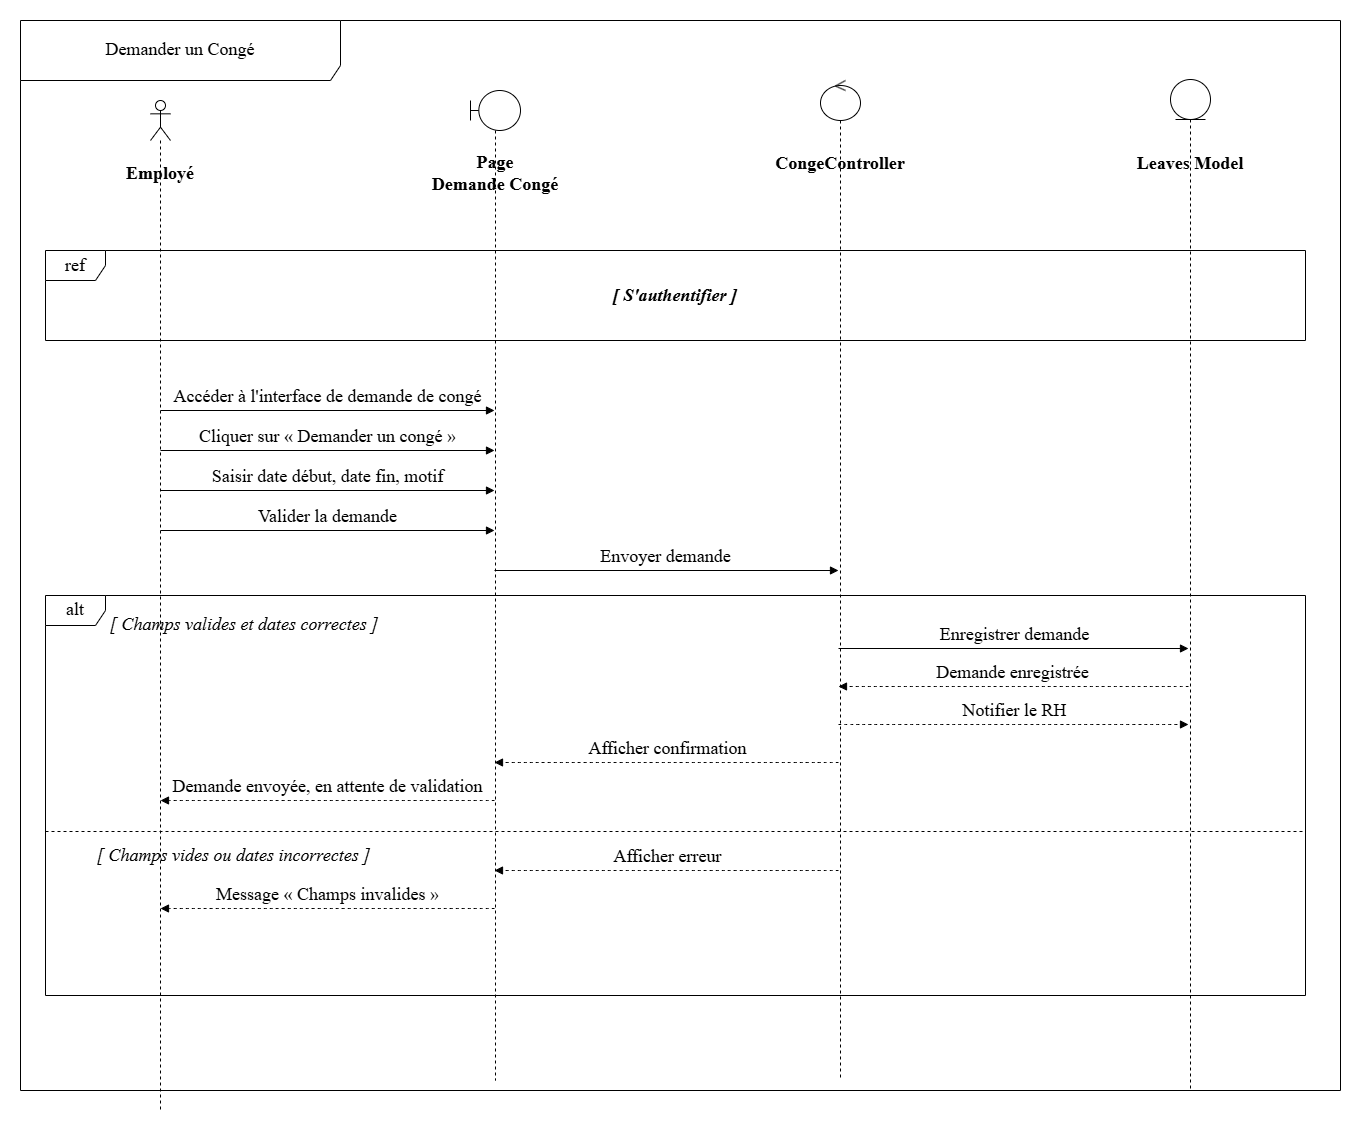
\includegraphics[width=0.9\textwidth]{projet/images/sequence s3/demander conges.drawio.png}
    \caption{Diagramme de séquence du cas d'utilisation «~Faire une demande de congé~»}
\end{figure}

\item[$\bullet$] \textbf{Diagramme de séquence du cas d'utilisation «~Déposer document~»}

Ce diagramme décrit le dépôt d'un document justificatif par l'employé. Il sélectionne le fichier à soumettre, saisit les informations nécessaires et le système enregistre le document avant de notifier le Responsable RH de son arrivée.

\begin{figure}[H]
    \centering
    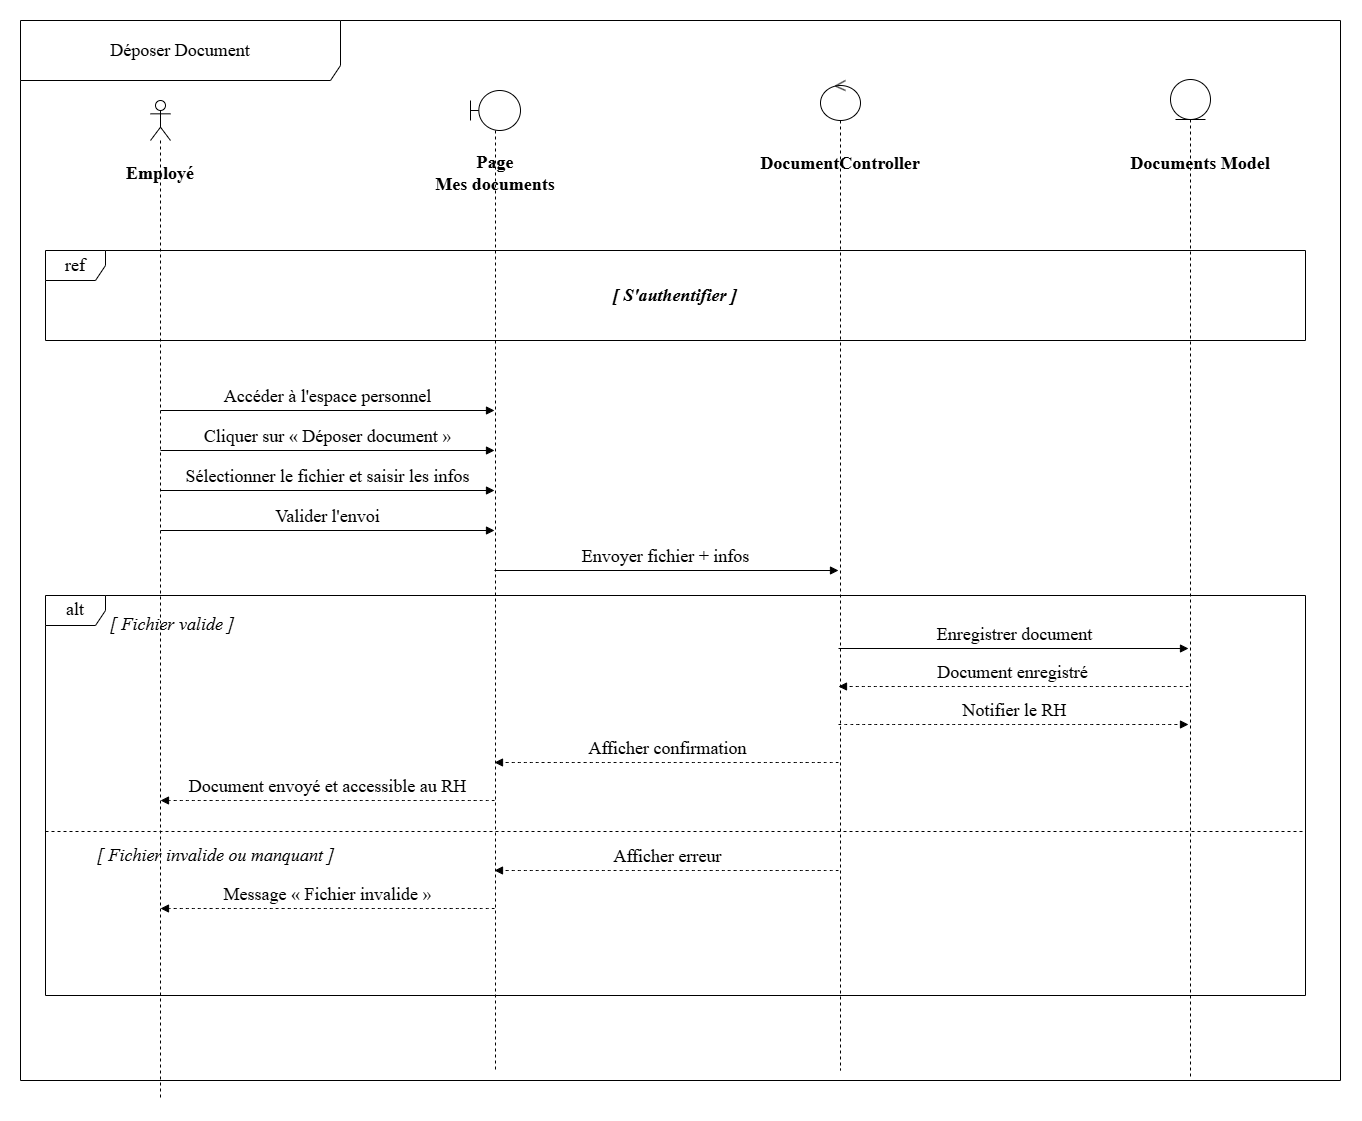
\includegraphics[width=0.9\textwidth]{projet/images/sequence s3/deposer documents.drawio.png}
    \caption{Diagramme de séquence du cas d'utilisation «~Déposer document~»}
\end{figure}

\end{itemize}

\subsubsection{Diagramme de classe de sprint 3}

Le diagramme de classe montre la structure des fonctionnalités de gestion des ressources humaines, notamment les congés, les documents administratifs, les primes, les déductions et les salaires des employés.

\begin{figure}[H]
    \centering
    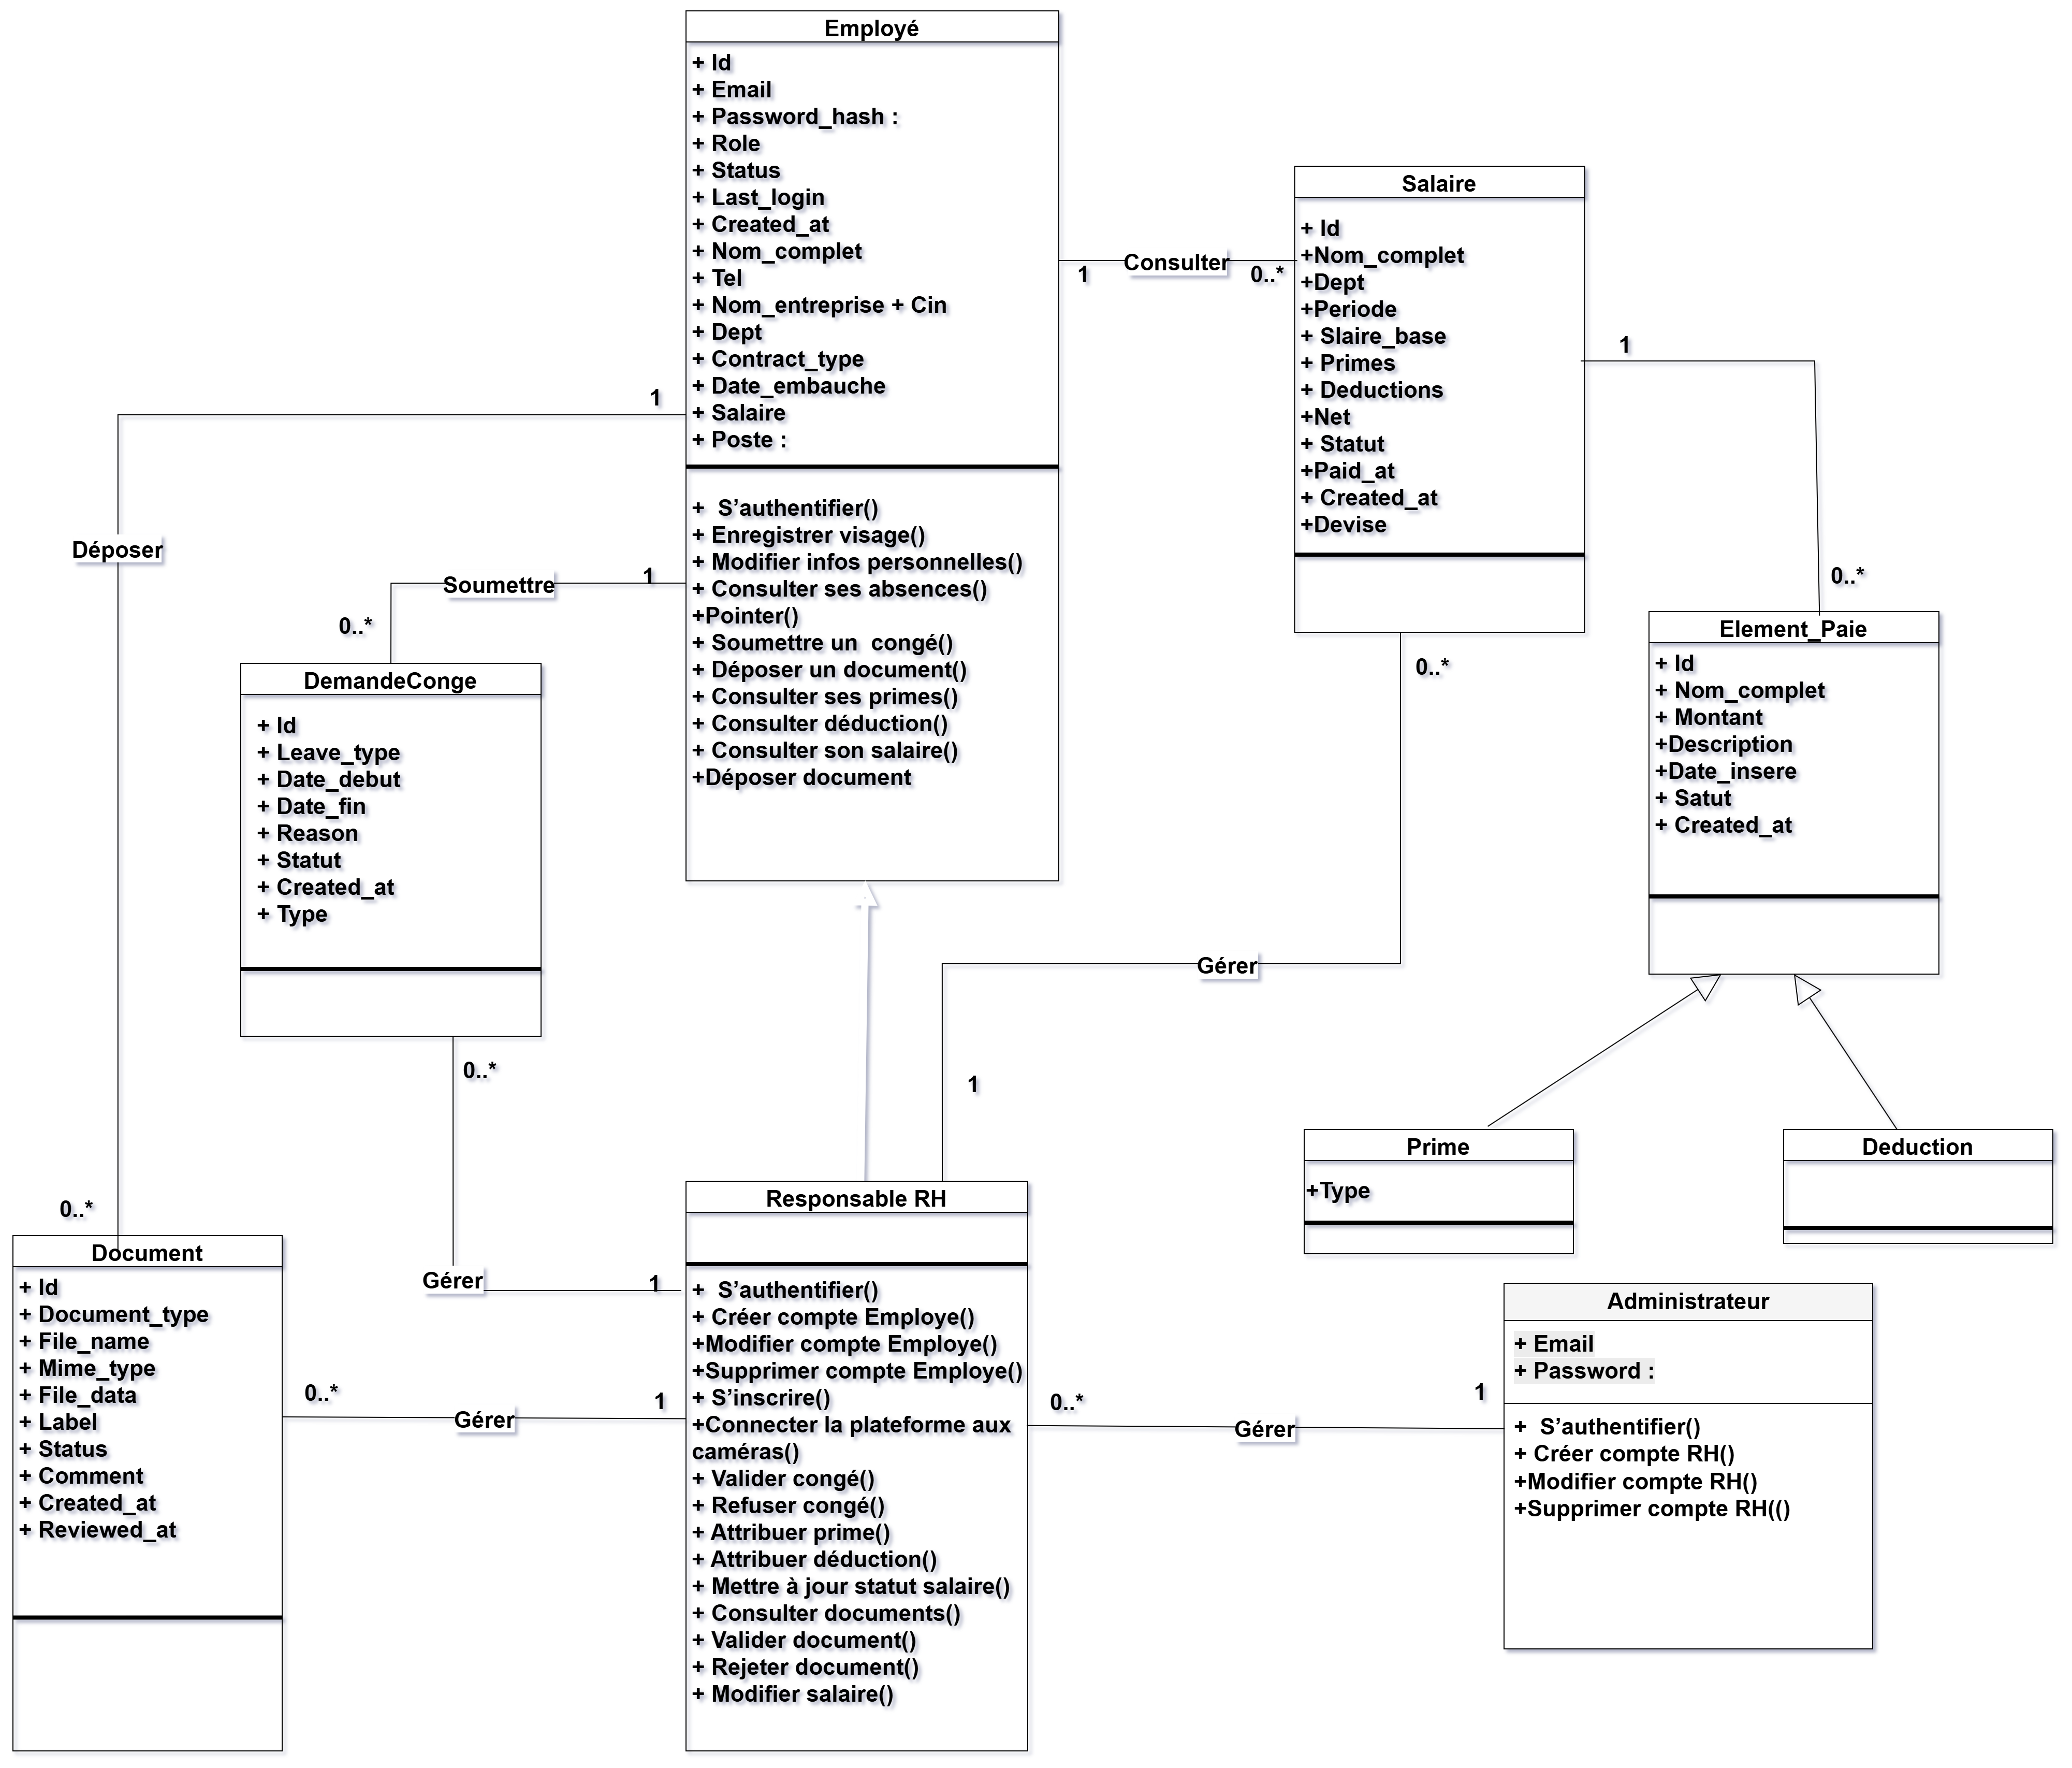
\includegraphics[width=0.9\textwidth]{projet/images/classe finale/s3.png}
    \caption{Diagramme de classe du sprint 3}
    \label{fig:classe_sprint3}
\end{figure}

\subsection{Interfaces réalisées pour le sprint 3}
\begin{itemize}

\item \textbf{Gestion des congés}

Cette interface permet au Responsable RH de consulter les demandes de congé soumises par les employés. Elle offre la possibilité de visualiser les détails de chaque demande, de l’approuver ou de la refuser tout en précisant, si nécessaire, le motif du refus.

\begin{figure}[H]
    \centering
    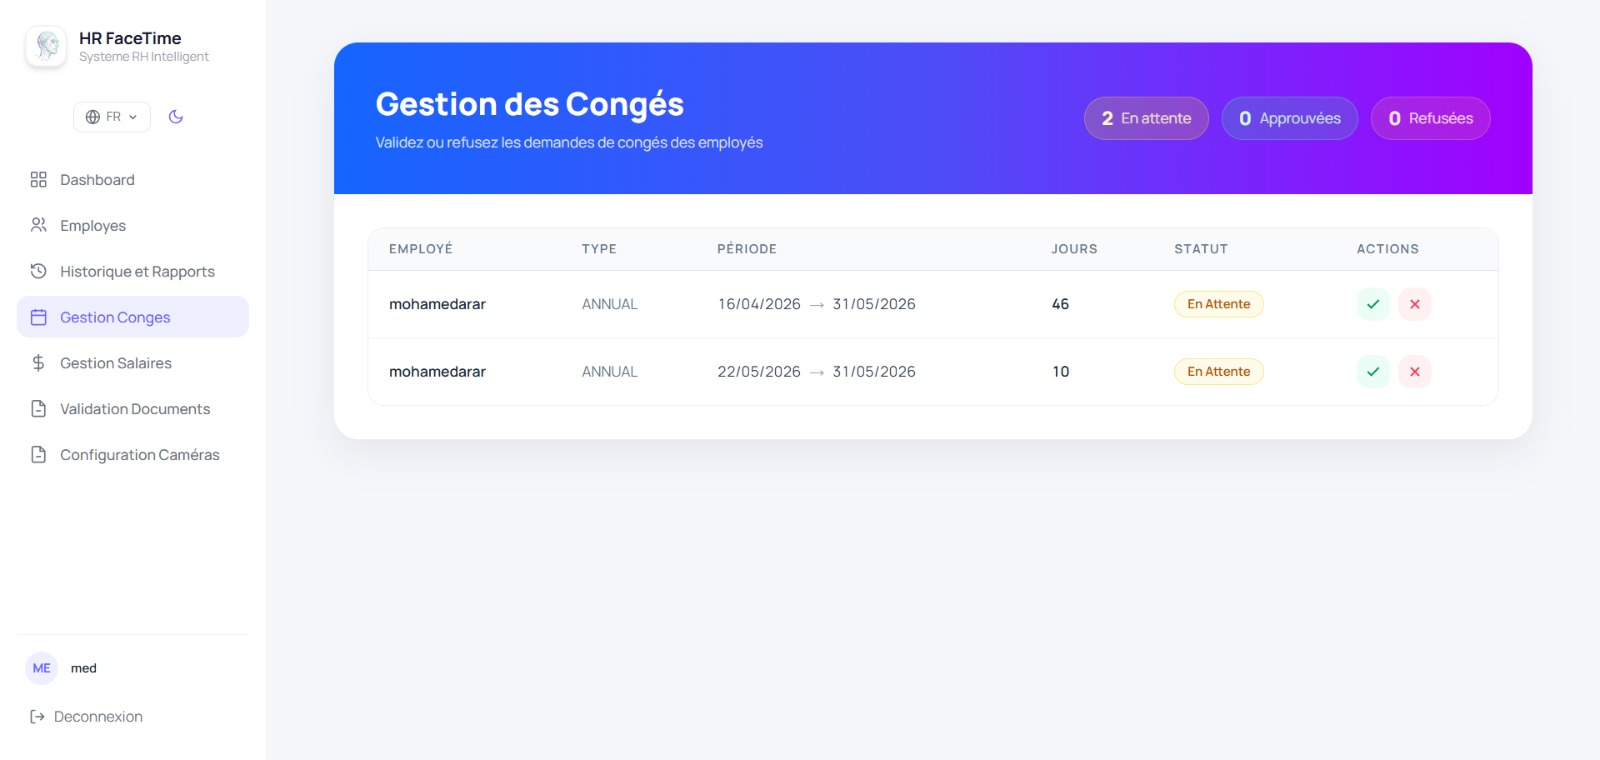
\includegraphics[width=0.9\textwidth]{projet/images/interface/s3/gestion_congee.jpeg}
    \caption{Gestion des congés}
\end{figure}

\item \textbf{Gestion des salaires}
Cette interface permet au Responsable RH de gérer les informations salariales des employés. Elle offre des fonctionnalités de modification du salaire de base, de mise à jour du statut de paiement et de suivi des opérations liées à la paie. Elle permet également l’attribution de primes ainsi que de déductions salariales.

\begin{figure}[H]
    \centering
    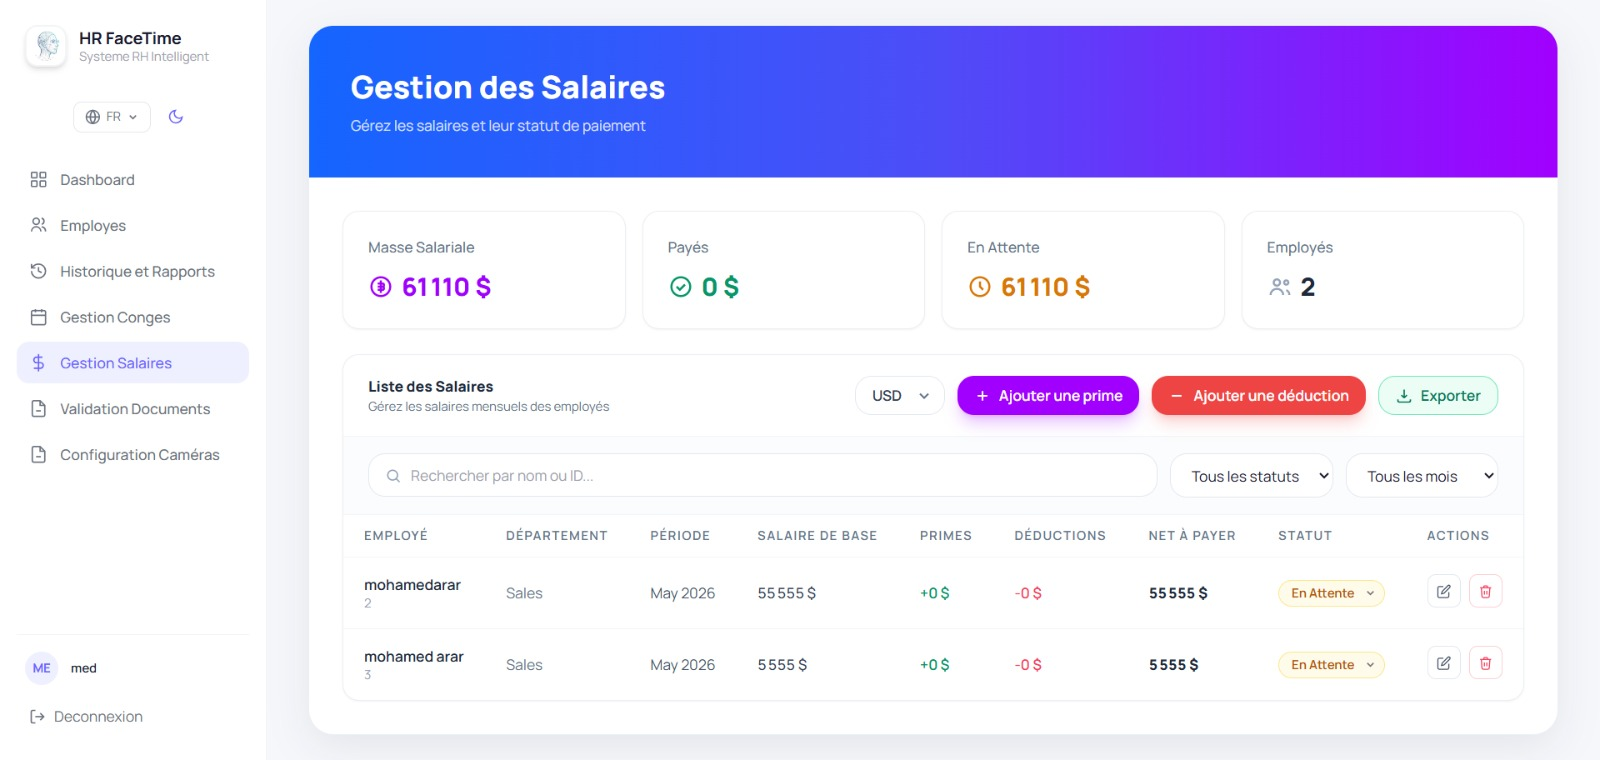
\includegraphics[width=0.9\textwidth]{projet/images/interface/s3/gestion_slaires.jpeg}
    \caption{Gestion des salaires}
\end{figure}



\item \textbf{Gestion des documents administratifs}

Cette interface permet au Responsable RH de consulter les documents déposés par les employés, d’accéder à leurs détails et de les valider ou de les rejeter selon leur conformité.

\begin{figure}[H]
    \centering
    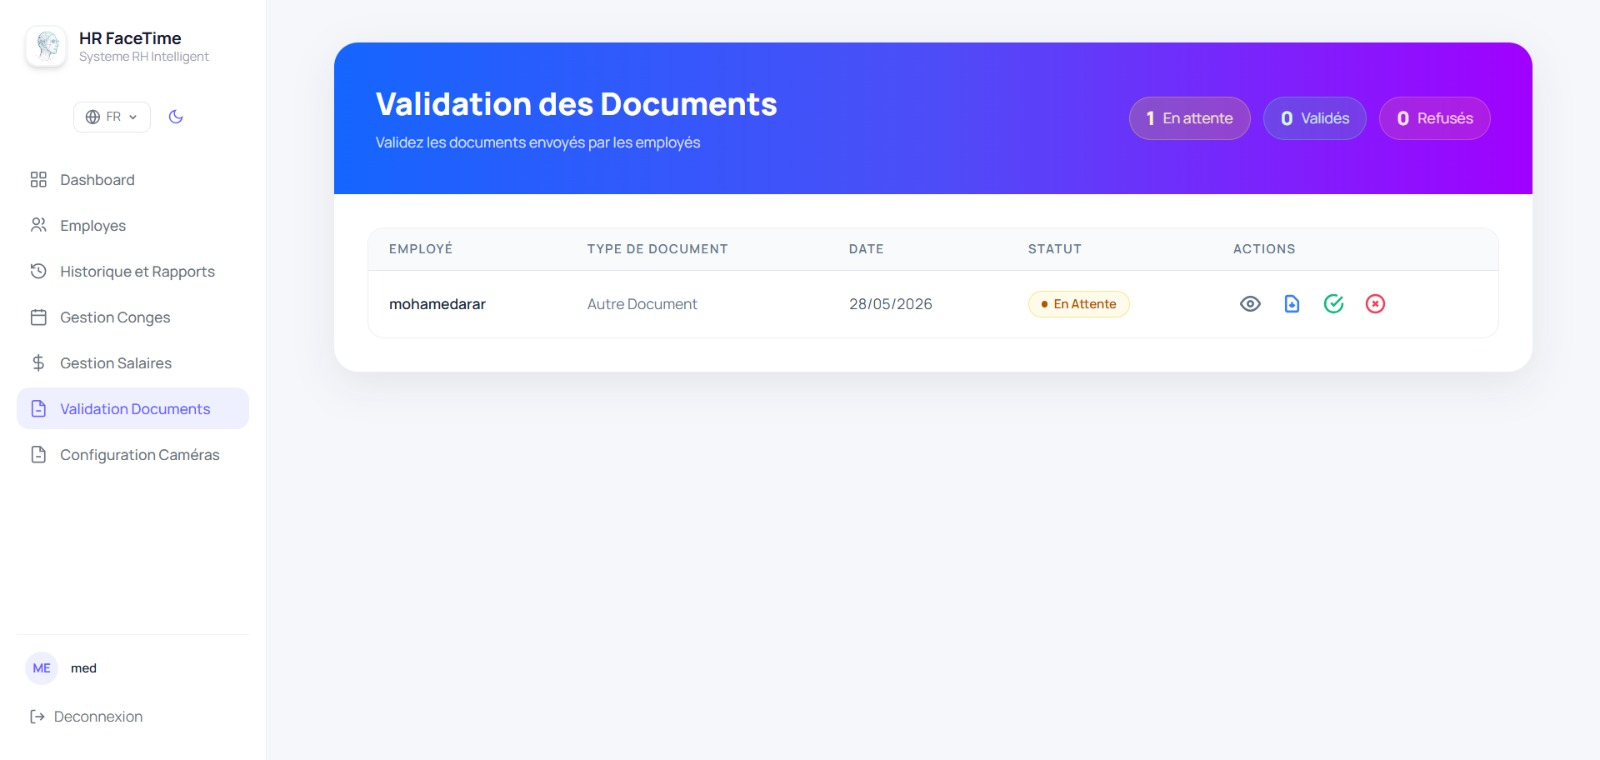
\includegraphics[width=0.9\textwidth]{projet/images/interface/s3/document.jpeg}
    \caption{Gestion des documents administratifs}
\end{figure}

\item \textbf{Mon salaire}

Cette interface permet à l’employé de consulter les informations relatives à sa rémunération, notamment le statut du salaire, les primes et les déductions associées.

\begin{figure}[H]
    \centering
    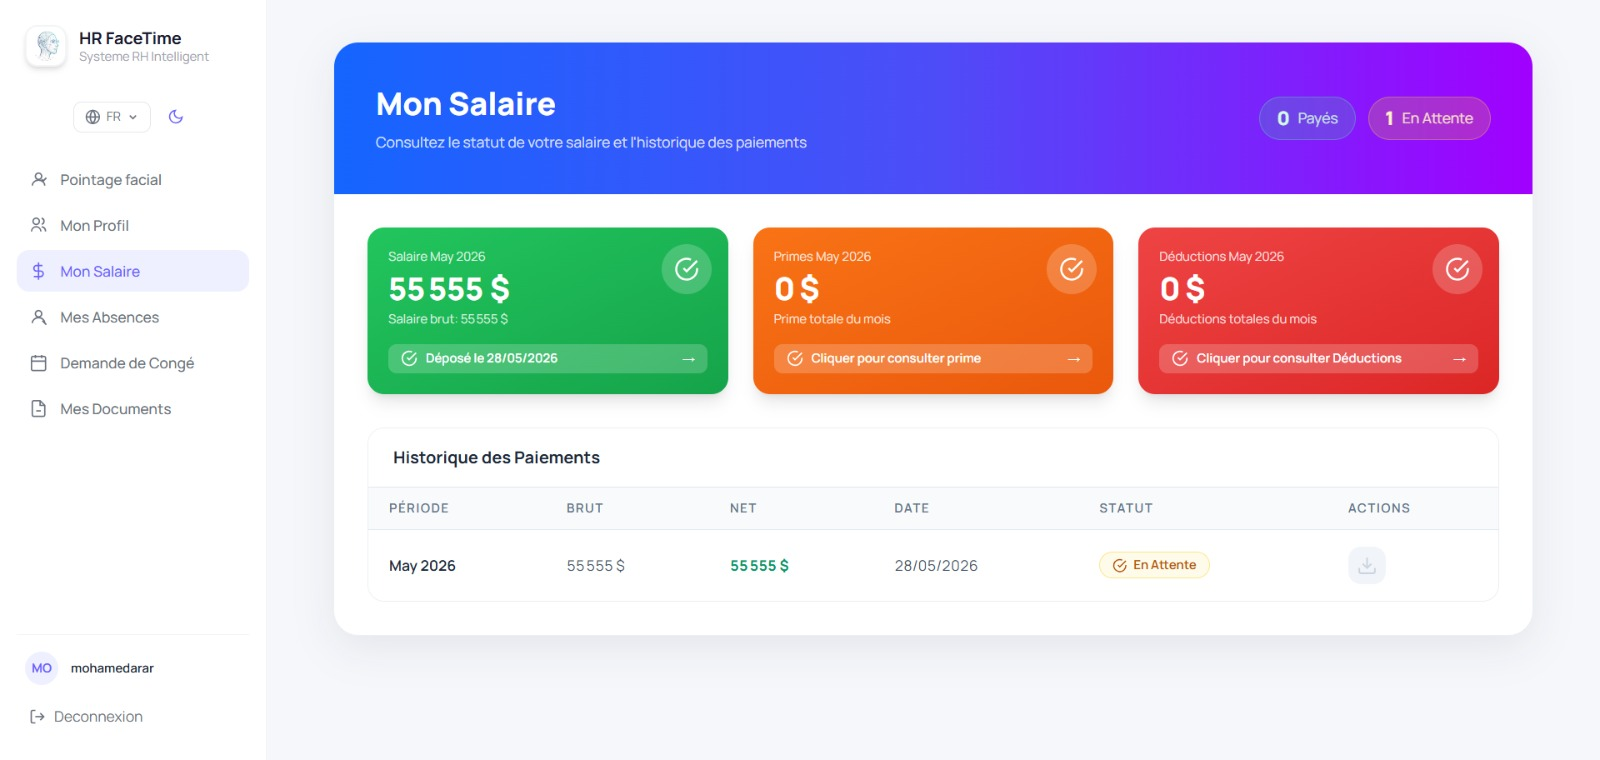
\includegraphics[width=0.9\textwidth]{projet/images/interface/s3/monsalaire.jpeg}
    \caption{Mon salaire}
\end{figure}

\item \textbf{Consultation des primes}

Cette interface permet à l’employé de visualiser l’ensemble des primes qui lui ont été attribuées ainsi que leurs montants et motifs.

\begin{figure}[H]
    \centering
    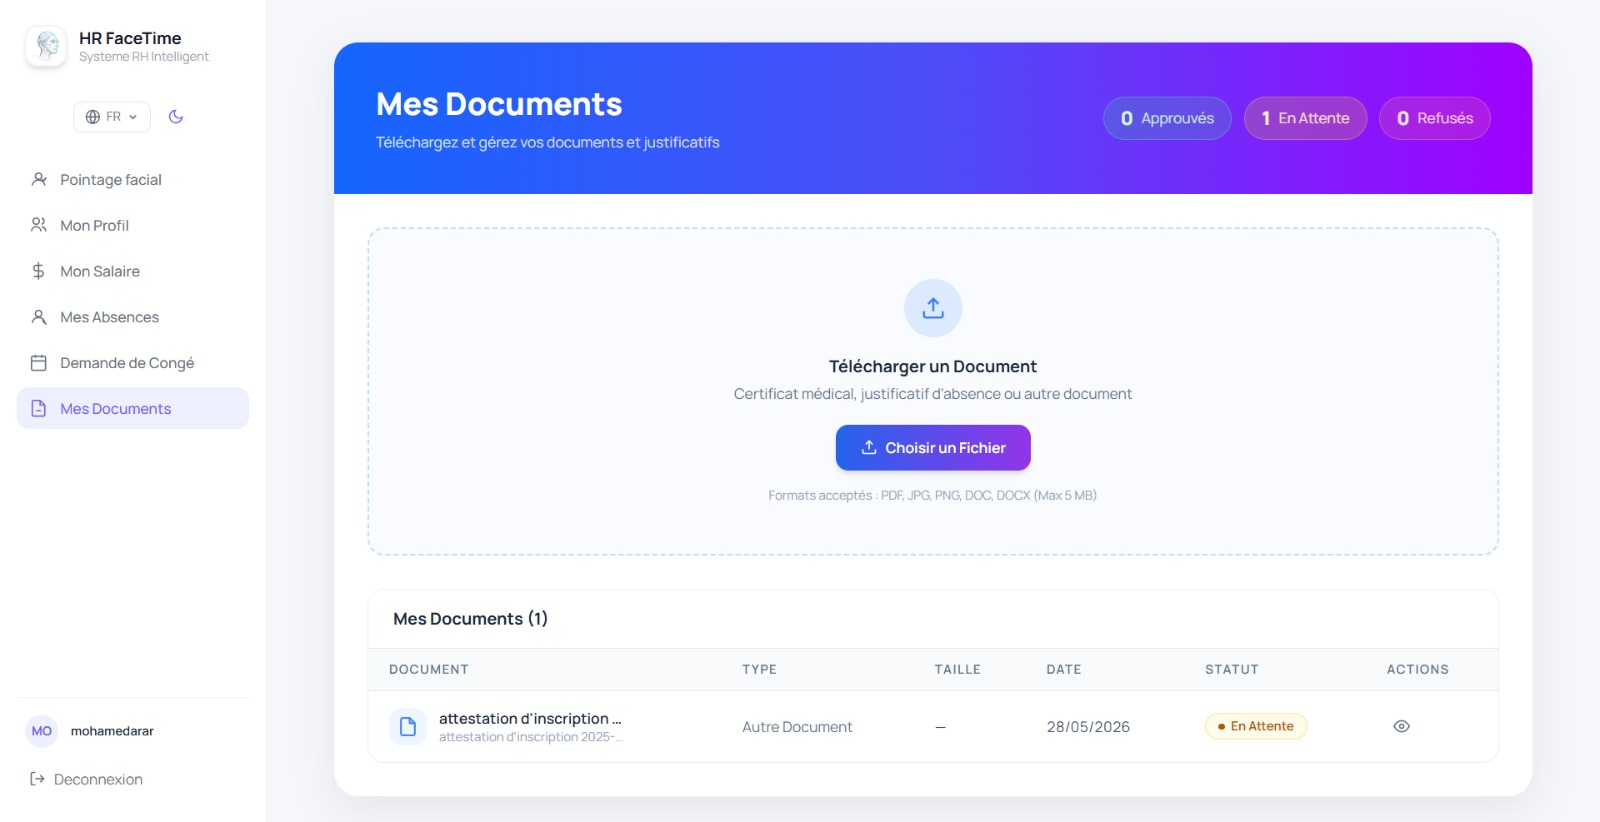
\includegraphics[width=0.9\textwidth]{projet/images/interface/s3/mes_document.jpeg}
    \caption{Consultation des primes}
\end{figure}

\item \textbf{Consultation des déductions}

Cette interface permet à l’employé de consulter les déductions appliquées à son salaire avec les montants et les motifs correspondants.

\begin{figure}[H]
    \centering
    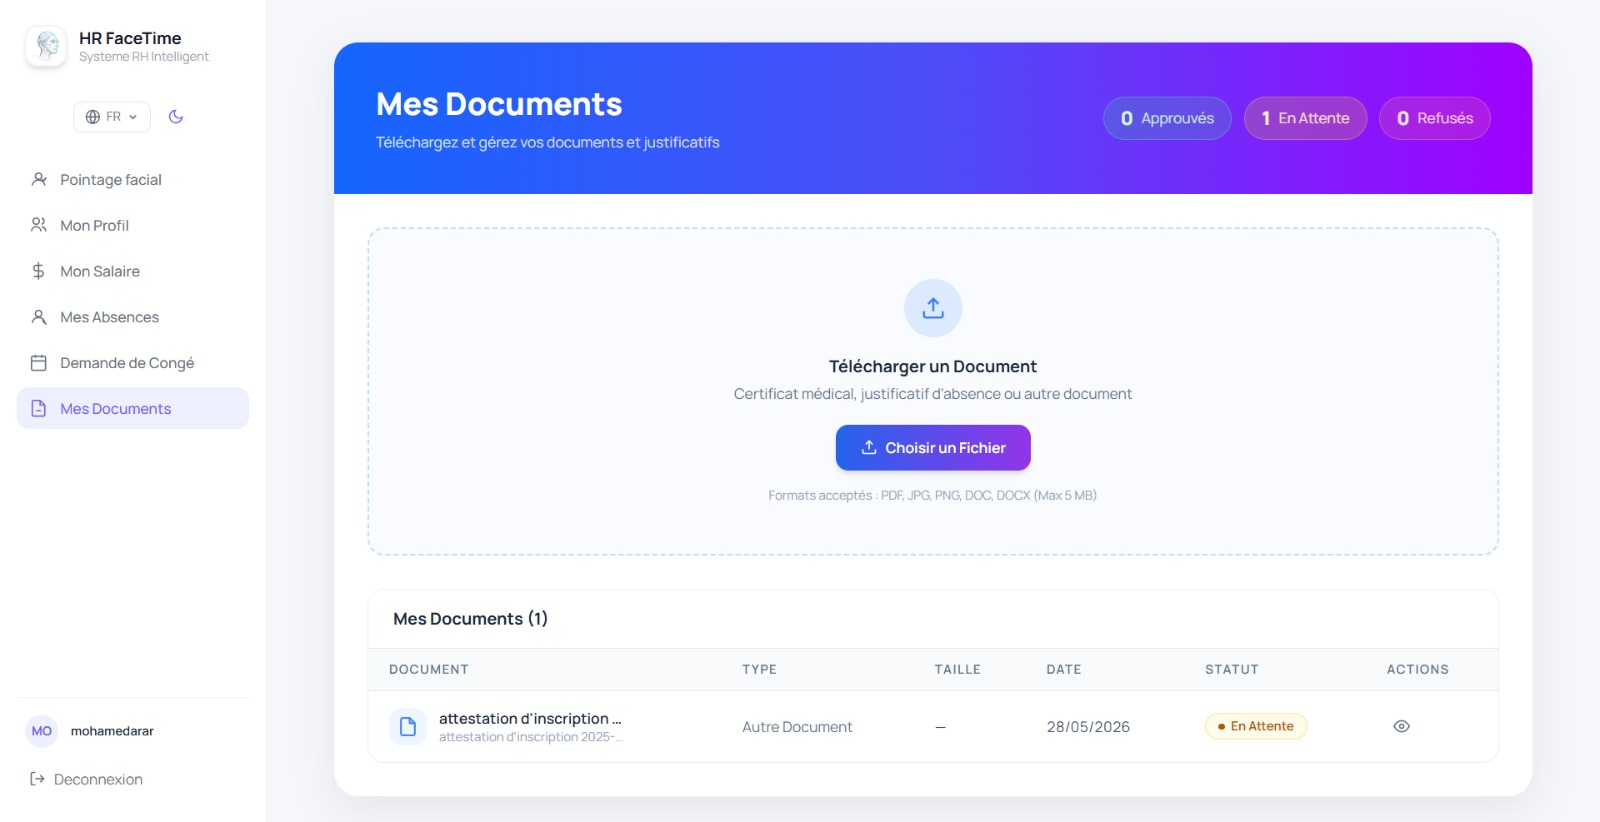
\includegraphics[width=0.9\textwidth]{projet/images/interface/s3/mes_document.jpeg}
    \caption{Consultation des déductions}
\end{figure}

\item \textbf{Demande de congé}

Cette interface permet à l’employé de soumettre une demande de congé en renseignant les dates concernées ainsi que le motif de l’absence.

\begin{figure}[H]
    \centering
    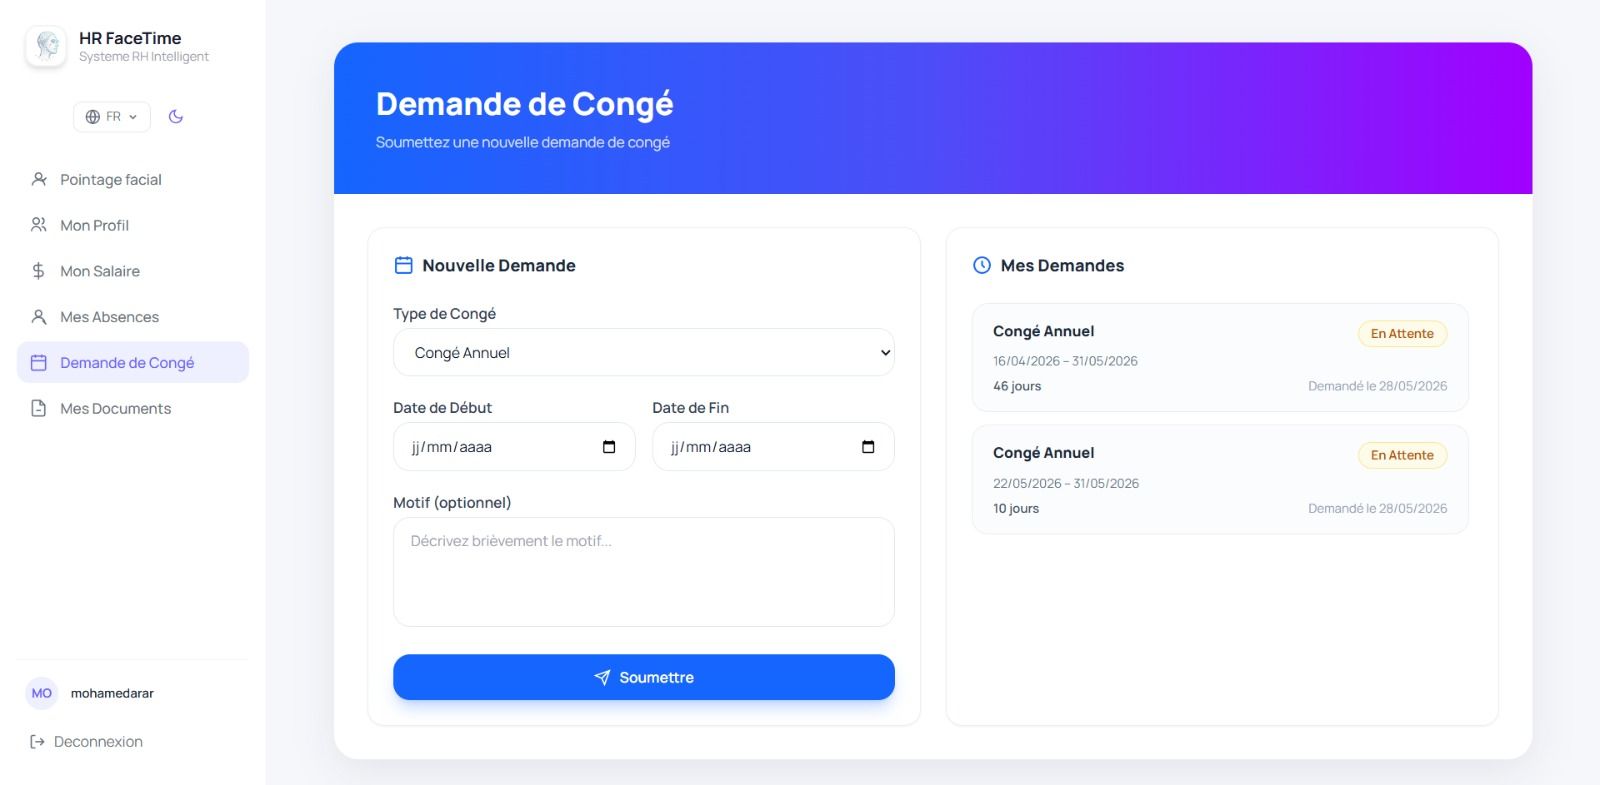
\includegraphics[width=0.9\textwidth]{projet/images/interface/s3/congeé.jpeg}
    \caption{Demande de congé}
\end{figure}

\item \textbf{Dépôt de document}

Cette interface permet à l’employé de déposer des documents administratifs ou justificatifs directement sur la plateforme afin qu’ils soient traités par le Responsable RH.

\begin{figure}[H]
    \centering
    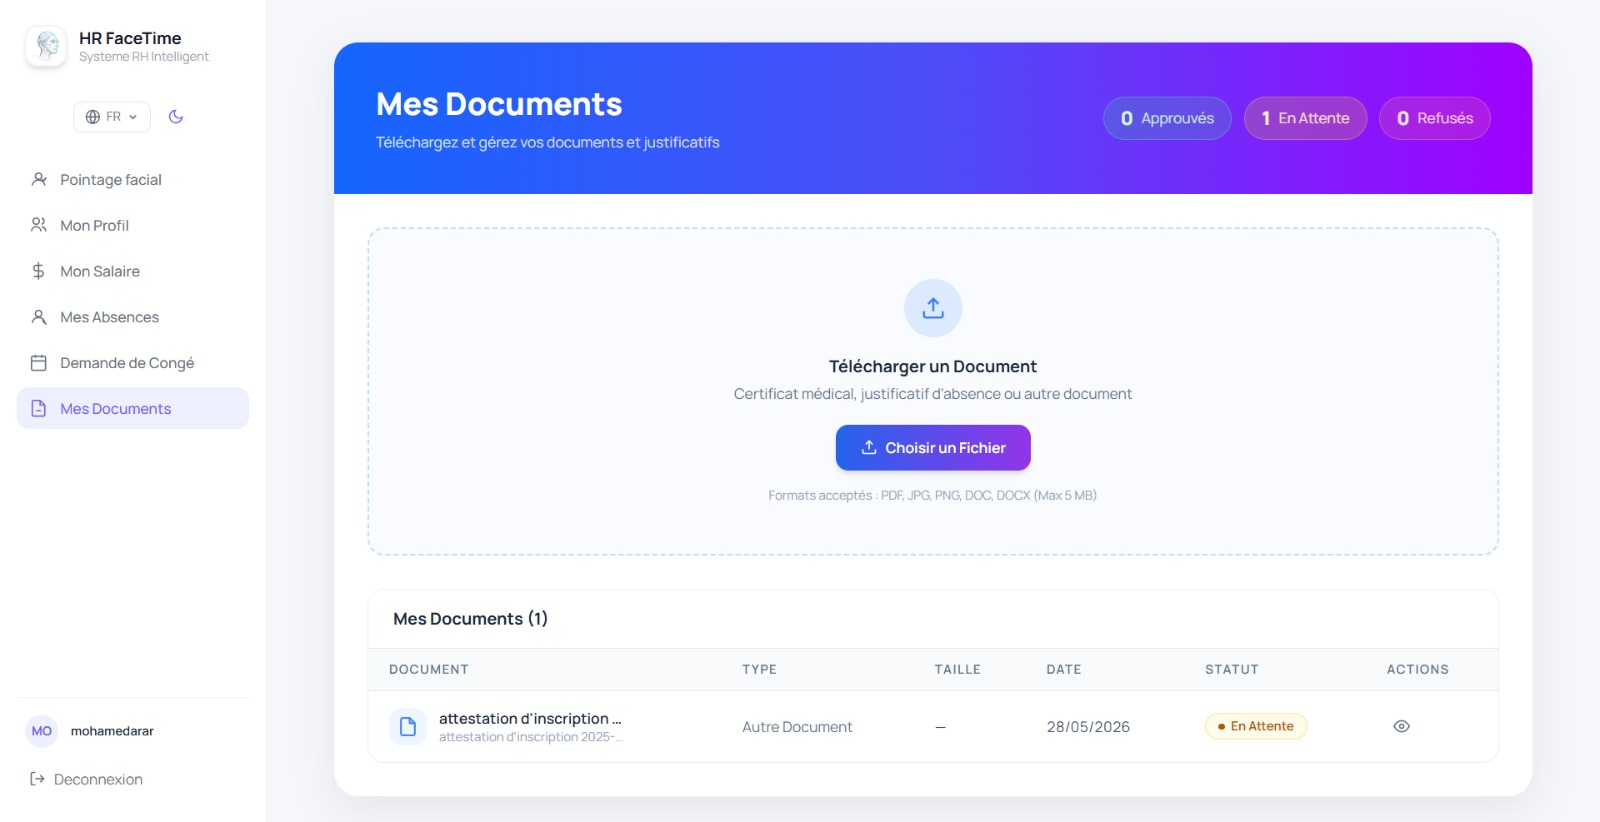
\includegraphics[width=0.9\textwidth]{projet/images/interface/s3/mes_document.jpeg}
    \caption{Dépôt de document}
\end{figure}

\end{itemize}
%==============================================================
\section{Sprint 4: Pilotage RH, Reporting, Paiement et Traçabilité}

Ce sprint a pour objectif de développer les outils de visualisation, paiement de frais permettant un pilotage global du système RH et le suivi des services de la plateforme.

\subsection{Objectif de sprint 4}
L'objectif de ce sprint est l'implémentation des tableaux de bord de l'Administrateur et du Responsable RH, la génération et la mise en export des rapports, ainsi que la gestion de la facturation du service.

\subsection{Durée de sprint 4}
\begin{itemize}
    \item \textbf{Date de début du sprint} : 03/05/2026
    \item \textbf{Date de fin du sprint} : 29/05/2026
\end{itemize}

\subsection{Backlog de sprint 4}
Le sprint backlog relatif à ce sprint est représenté dans le tableau ci-joint.
\begin{longtable}{|>{\centering\arraybackslash}m{0.5cm}|
    >{\centering\arraybackslash}m{3cm}|
    >{\centering\arraybackslash}m{2.5cm}|
    >{\centering\arraybackslash}m{3cm}|
    >{\centering\arraybackslash}m{3cm}|
    >{\centering\arraybackslash}m{0.7cm}|
    >{\centering\arraybackslash}m{0.9cm}|}
\hline
\textbf{ID} & \textbf{User Story} & \textbf{En tant que} & \textbf{Je veux} & \textbf{Afin de} & \textbf{P} & \textbf{C} \\
\hline
4  & Visualiser Dashboard Admin       & Administrateur   & surveiller le système                       & assurer la stabilité          & 5 & 4 \\ \hline
6  & Visualiser Dashboard RH          & Responsable RH   & visualiser les indicateurs RH               & piloter l'activité RH         & 5 & 3 \\ \hline
20 & Générer rapport                 & Responsable RH   & générer des rapports                        & analyser les données RH       & 3 & 3 \\ \hline

21 & Consulter historique             & Responsable RH   & consulter l'historique des actions RH       & assurer la traçabilité        & 4 & 3 \\ \hline


\caption{Backlog Sprint 4 --- Pilotage RH, Reporting \& Gestion des Paiements}
\end{longtable}

\subsection{Spécification fonctionnelle détaillée}

\begin{itemize}

\item \textbf{Diagramme de cas d'utilisation du sprint 4}

\begin{figure}[H]
    \centering
    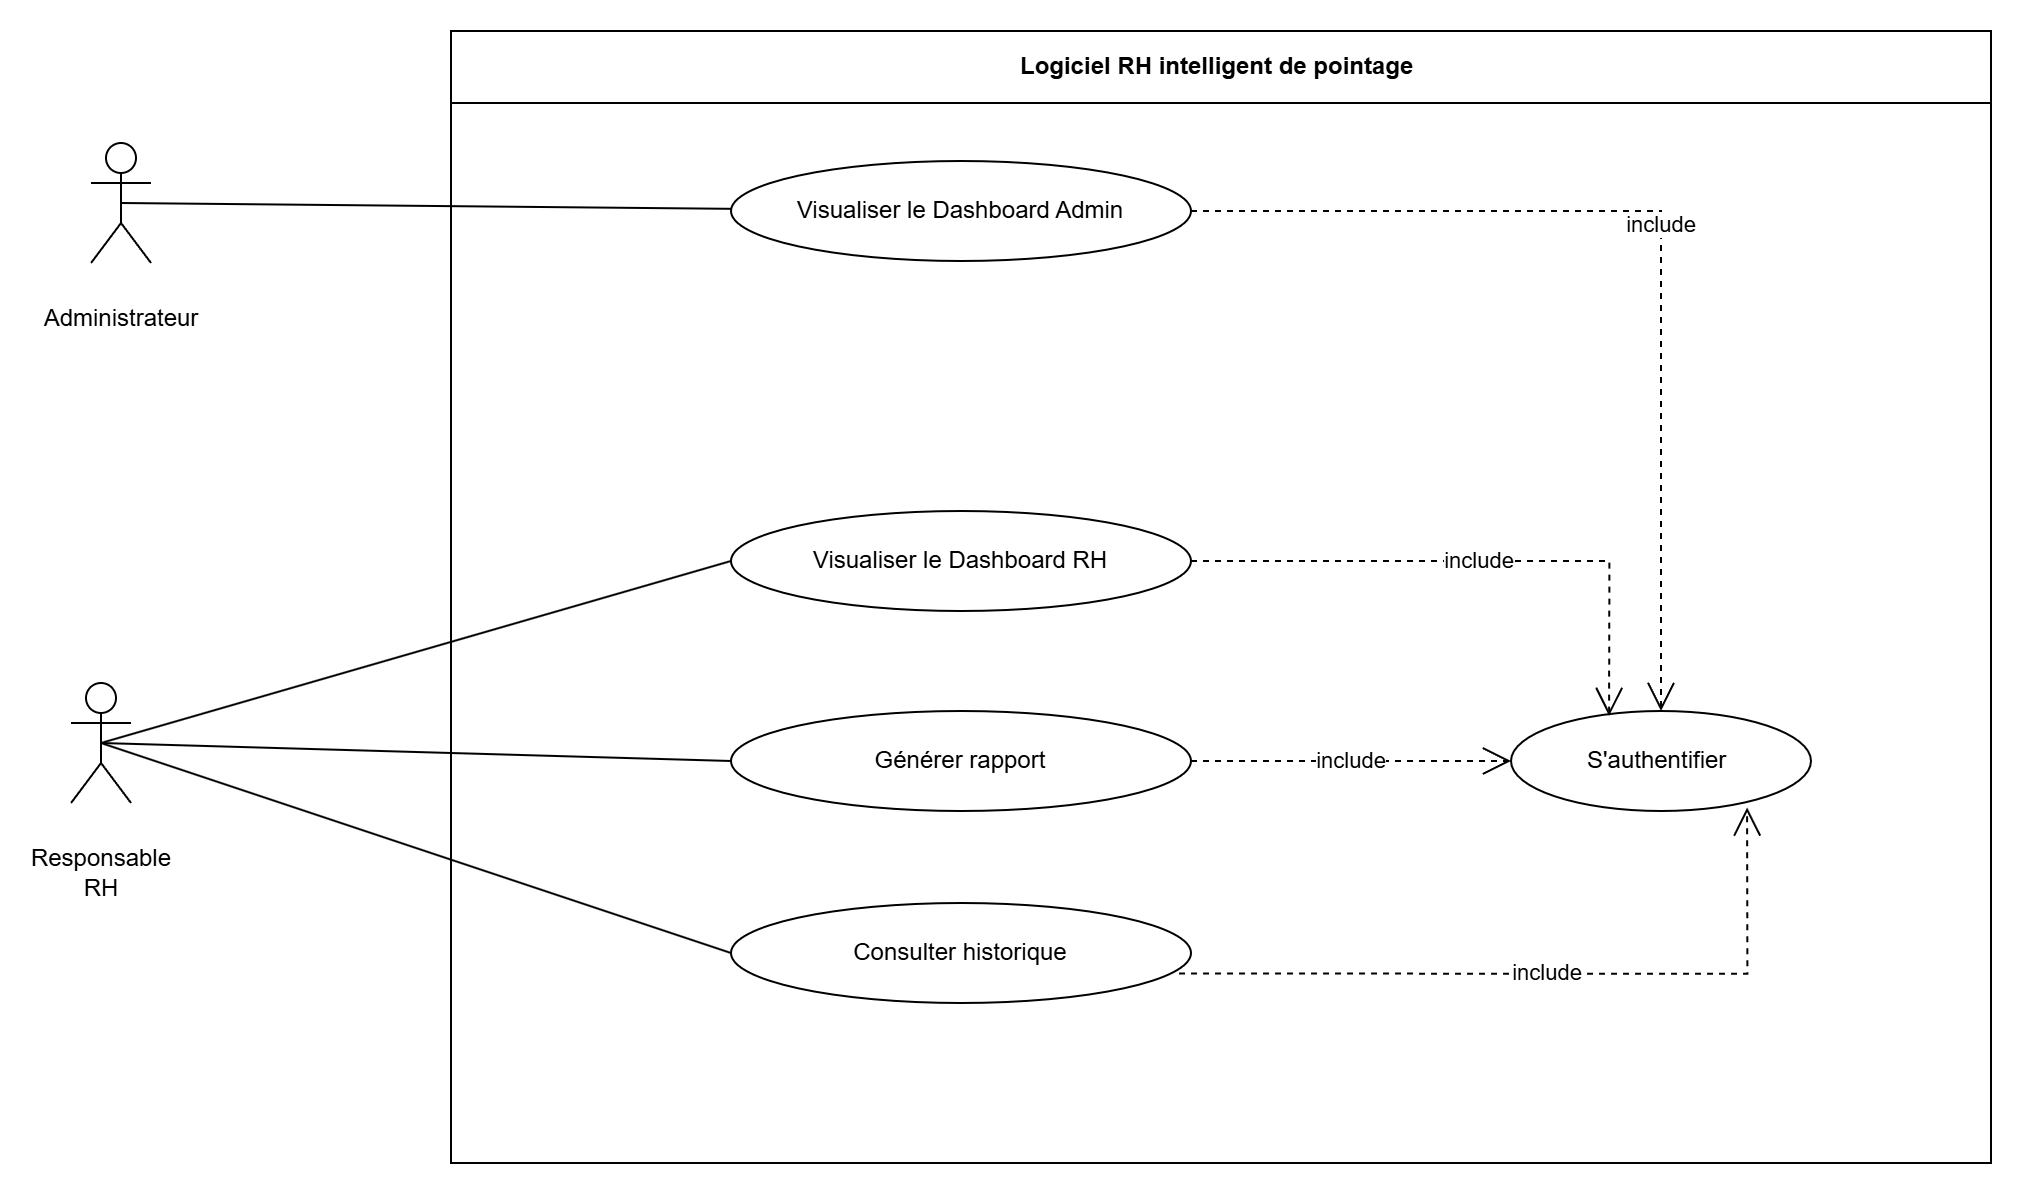
\includegraphics[width=0.9\textwidth]{projet/images/usecase/sprint 4/uses4.drawio.png}
    \caption{Diagramme de Cas d'utilisation du Sprint 4}
    \label{fig:usecase_sprint4}
\end{figure}

\item \textbf{Description textuelle : cas d'utilisation «~Visualiser le Dashboard Administrateur~»}

\begin{center} \begin{longtable}{|p{5cm}|p{11cm}|} \hline \textbf{Nom du cas d'utilisation} & Visualiser tableau de bord administrateur \\ \hline \textbf{Acteurs} & Administrateur \\ \hline \textbf{Objectif} & Permettre à l’administrateur de visualiser le tableau de bord du système \\ \hline \textbf{Préconditions} & L’administrateur est déjà authentifié dans le système \\ \hline \textbf{Scénario nominal} & 1. L’administrateur accède à l’application. \newline 2. Le système détecte une session administrateur active. \newline 3. Le système charge automatiquement les données nécessaires. \newline 4. Le tableau de bord administrateur s’affiche avec les différentes fonctionnalités disponibles. \\ \hline \textbf{Scénario d'exception} & Session inexistante ou expirée $\rightarrow$ redirection vers la page de connexion. \\ \hline \textbf{Post-condition} & Le tableau de bord administrateur est affiché et prêt à être utilisé. \\ \hline \caption{Description textuelle du cas d'utilisation «~Visualiser tableau de bord administrateur~»} \end{longtable} \end{center}


\item \textbf{Description textuelle : cas d'utilisation «~Visualiser le Dashboard RH~»}

\begin{center} \begin{longtable}{|p{5cm}|p{11cm}|} \hline \textbf{Nom du cas d'utilisation} & Visualiser tableau de bord RH \\ \hline \textbf{Acteurs} & Responsable RH \\ \hline \textbf{Objectif} & Permettre au responsable RH de visualiser le tableau de bord des ressources humaines \\ \hline \textbf{Préconditions} & Le responsable RH est déjà authentifié dans le système \\ \hline \textbf{Scénario nominal} & 1. Le responsable RH accède à l’application. \newline 2. Le système détecte une session RH active. \newline 3. Le système charge automatiquement les données et fonctionnalités RH. \newline 4. Le tableau de bord RH s’affiche avec les différentes options disponibles. \\ \hline \textbf{Scénario d'exception} & Session inexistante ou expirée $\rightarrow$ redirection vers la page de connexion. \\ \hline \textbf{Post-condition} & Le tableau de bord RH est affiché et prêt à être utilisé. \\ \hline \caption{Description textuelle du cas d'utilisation «~Visualiser tableau de bord RH~»} \end{longtable} \end{center}



\item \textbf{Description textuelle : cas d'utilisation «~Consulter historique~»}

\begin{center}
\begin{longtable}{|p{5cm}|p{11cm}|}
\hline

\textbf{Nom du cas d'utilisation} & Exporter l'historique \\ \hline

\textbf{Acteurs} & Responsable RH \\ \hline

\textbf{Objectif} & Permettre au responsable RH d’exporter l’historique des absences sous forme de fichier \\ \hline

\textbf{Préconditions} & Responsable RH authentifié et historique déjà consulté \\ \hline

\textbf{Scénario nominal} &
1. Accéder à l’interface de l’historique. \newline
2. Afficher les données sous forme de tableau. \newline
3. Cliquer sur le bouton « Exporter ». \newline
4. Choisir le format (PDF ou Excel). \newline
5. Le système génère le fichier. \newline
6. Téléchargement automatique du fichier. \\ \hline

\textbf{Scénario d'exception} &
Erreur de génération $\rightarrow$ message « Export impossible ». \\ \hline

\textbf{Post-condition} &
Le fichier d’historique est exporté et disponible sur l’appareil. \\ \hline

\caption{Description textuelle du cas d'utilisation «~Exporter l'historique~»}
\end{longtable}
\end{center}

\item \textbf{Description textuelle : cas d'utilisation «~Exporter rapport~»}

\begin{center}
\begin{longtable}{|p{5cm}|p{11cm}|}
\hline

\textbf{Nom du cas d'utilisation} & Exporter rapport \\ \hline

\textbf{Acteurs} & Responsable RH \\ \hline

\textbf{Objectif} & Générer et exporter un rapport RH \\ \hline

\textbf{Préconditions} & Responsable RH authentifié \\ \hline

\textbf{Scénario nominal} &
1. Accéder à l’interface principale. \newline
2. Cliquer sur le menu « Historique ». \newline
3. Accéder à la section « Rapports et Analytics ». \newline
4. Sélectionner le type de rapport et la période souhaitée. \newline
5. Cliquer sur le bouton « Exporter ». \newline
6. Le système génère automatiquement le rapport. \newline
7. Le fichier est téléchargé pour consultation. \\ \hline

\textbf{Scénario d'exception} &
Erreur lors de la génération ou de l’exportation $\rightarrow$ message « Export impossible ». \\ \hline

\textbf{Post-condition} &
Le rapport est généré et disponible pour consultation ou téléchargement. \\ \hline

\caption{Description textuelle du cas d'utilisation «~Exporter rapport~»}
\end{longtable}
\end{center}



\end{itemize}

\subsection{Conception}
\subsubsection{Diagrammes de séquence}

\begin{itemize}

\item[$\bullet$] \textbf{Diagramme de séquence du cas d'utilisation «~Visualiser le Dashboard (Administrateur)~»}



% NOTE: image manquante dans le source original — à compléter
\begin{figure}[H]
    \centering
    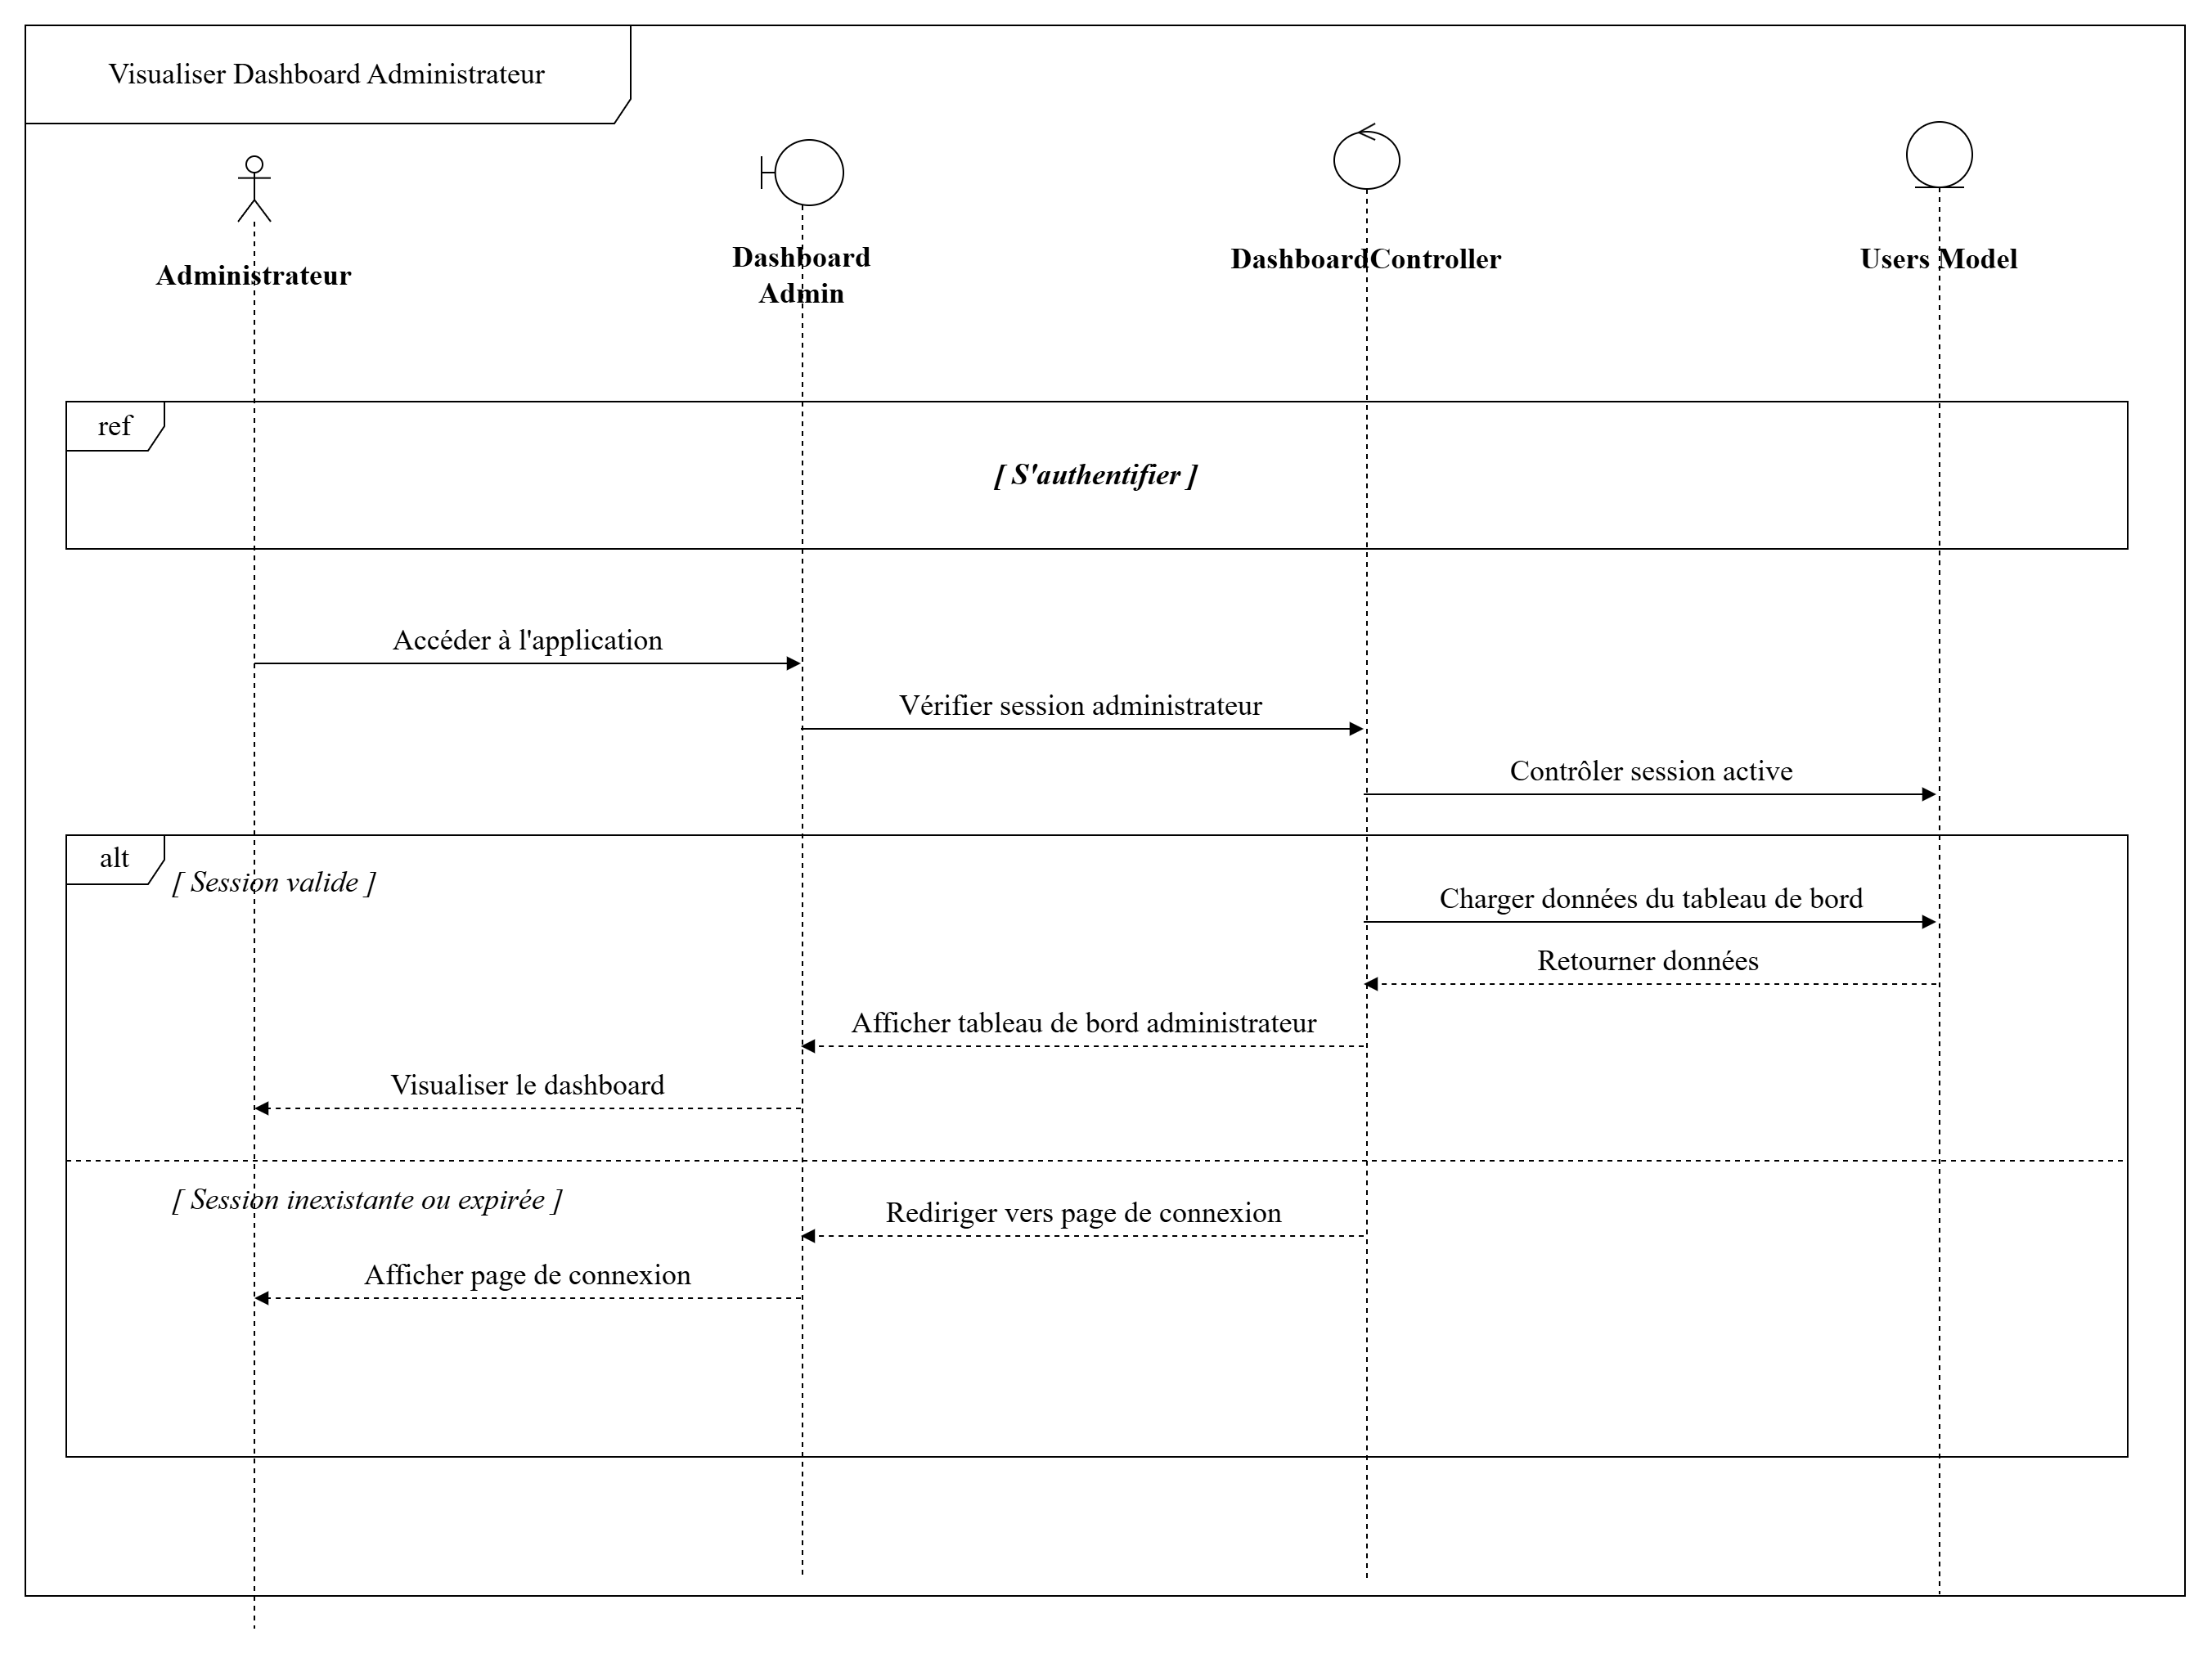
\includegraphics[width=0.9\textwidth]{projet/images/sequence s4/dachbordad.drawio.png}
    \caption{Diagramme de séquence du cas d'utilisation «~Visualiser le Dashboard (Responsable Administrateur )»}
\end{figure}

\item[$\bullet$] \textbf{Diagramme de séquence du cas d'utilisation «~Visualiser le Dashboard (Responsable RH)~»}



\begin{figure}[H]
    \centering
    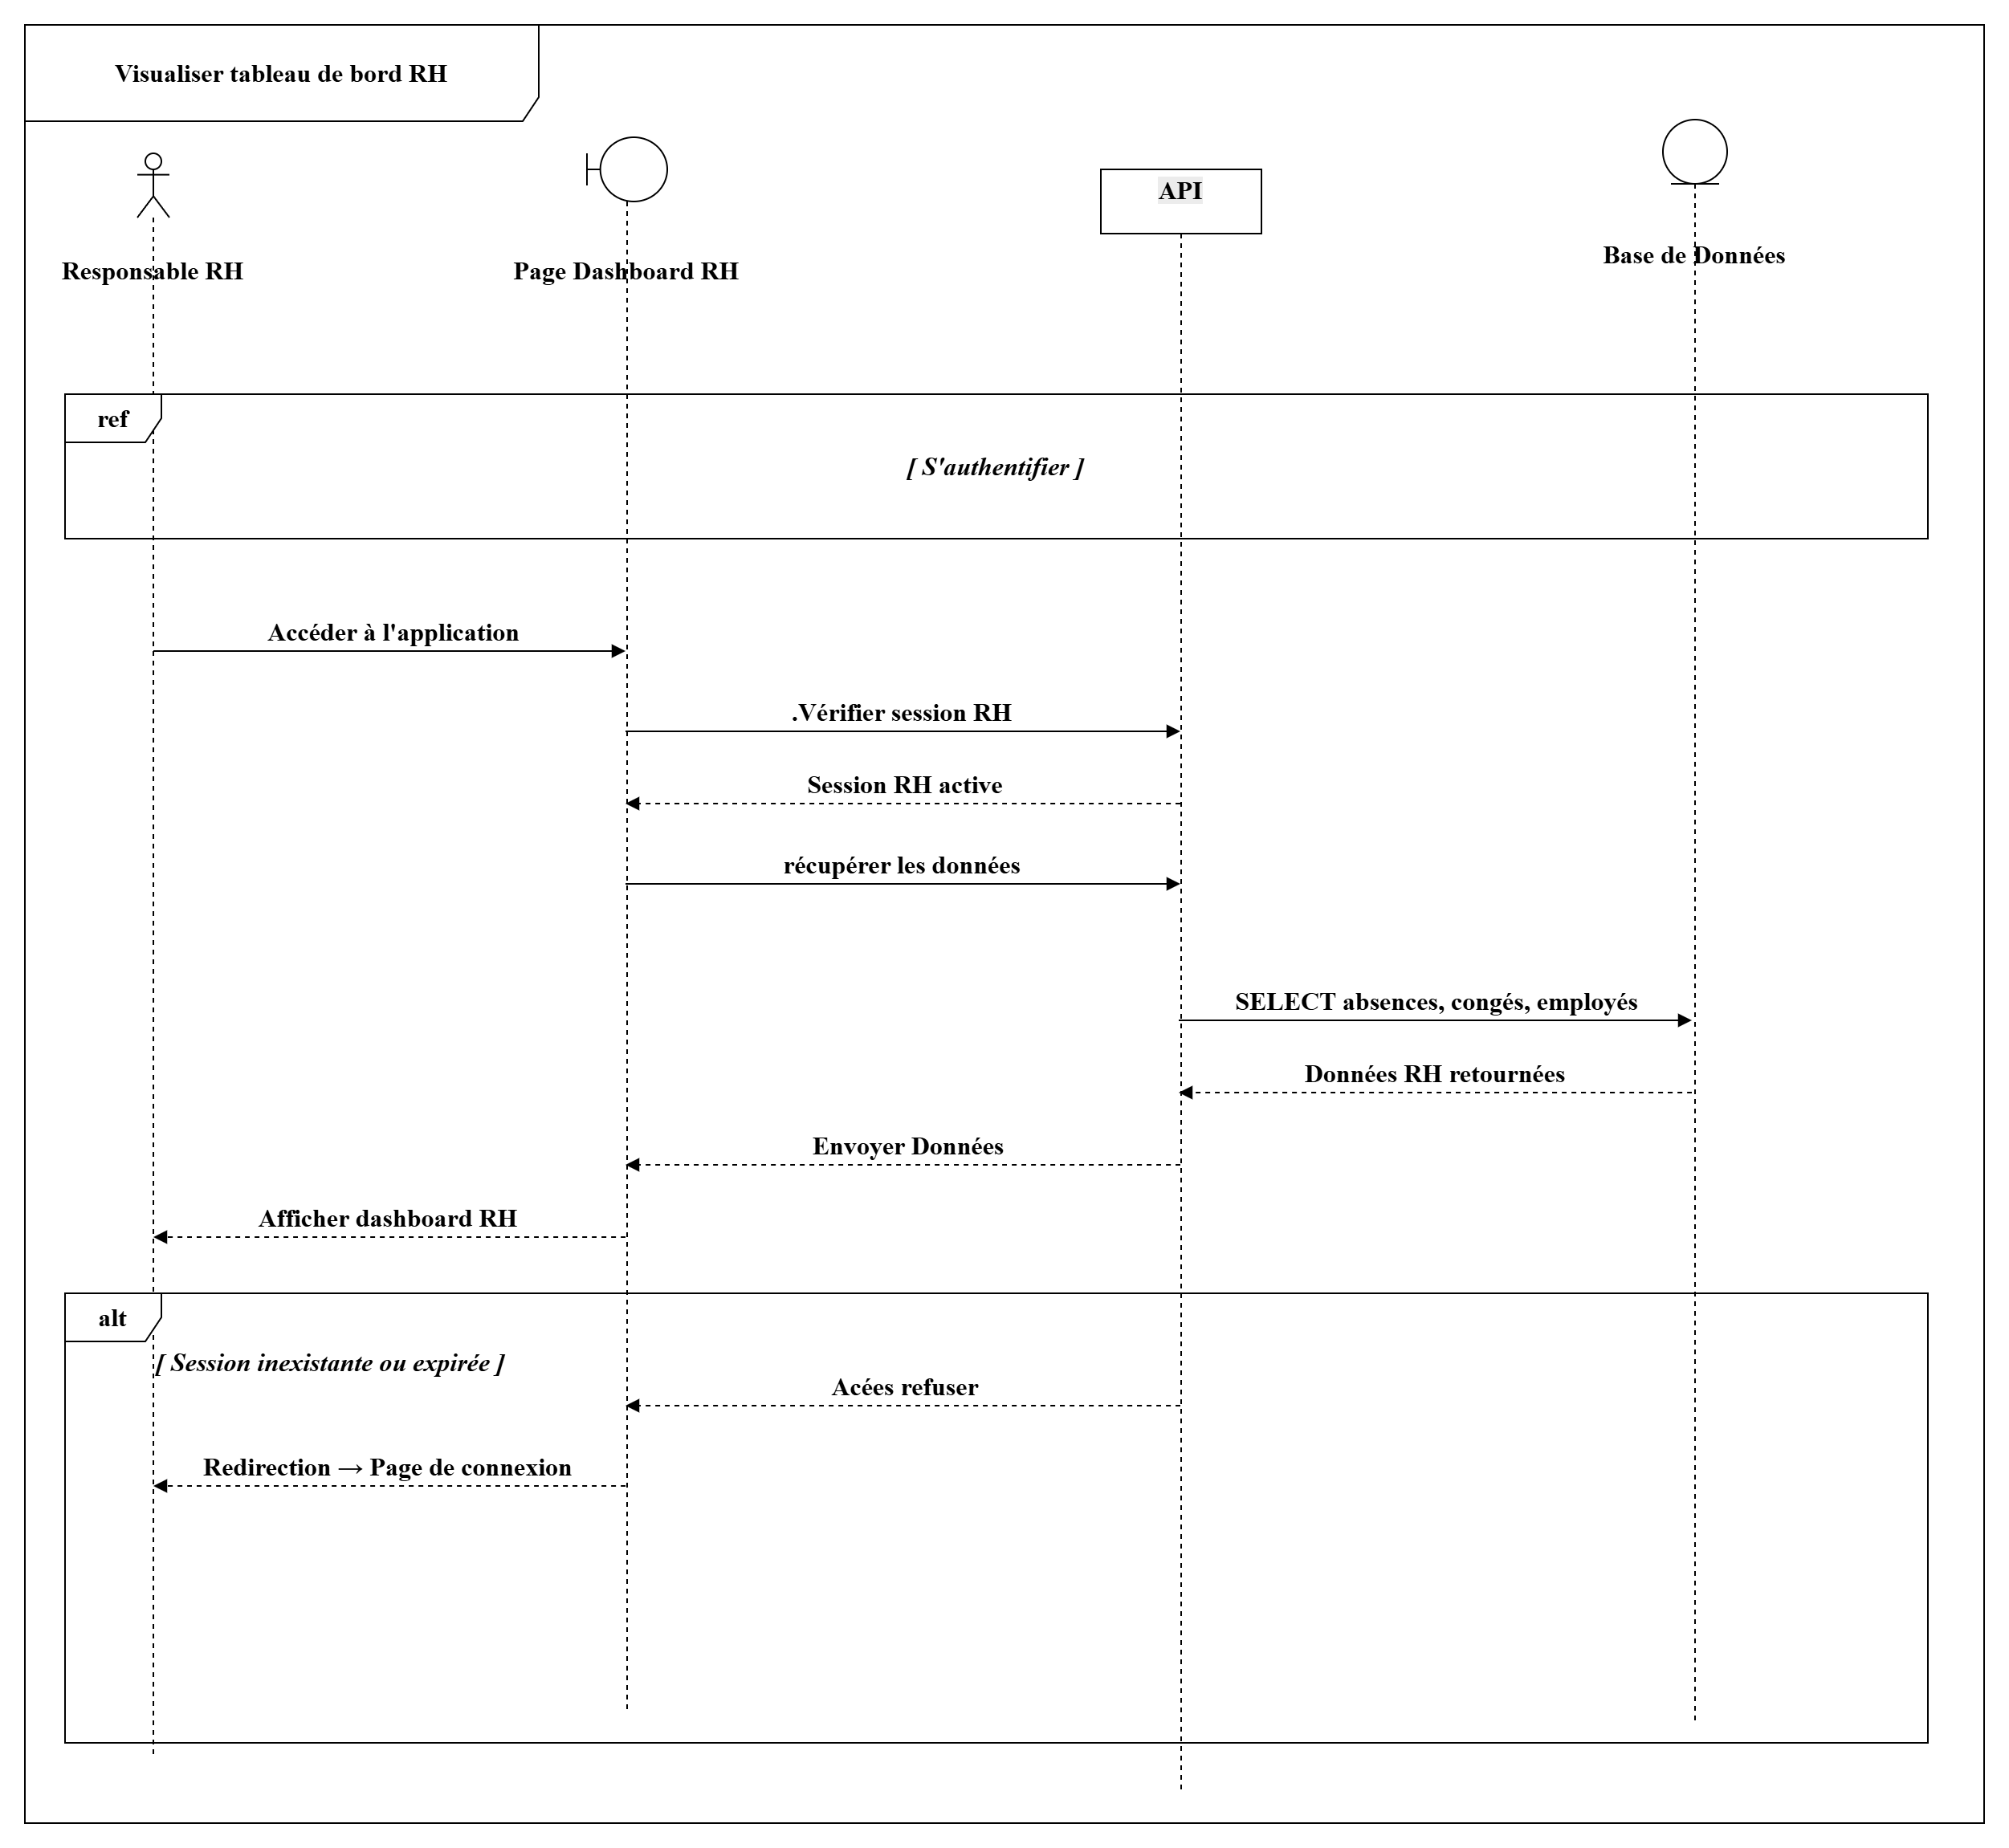
\includegraphics[width=0.9\textwidth]{projet/images/sequence s4/bash rh.drawio.png}
    \caption{Diagramme de séquence du cas d'utilisation «~Visualiser le Dashboard (Responsable RH)~»}
\end{figure}


\item[$\bullet$] \textbf{Diagramme de séquence du cas d'utilisation «Consulter historique »}



\begin{figure}[H]
    \centering
    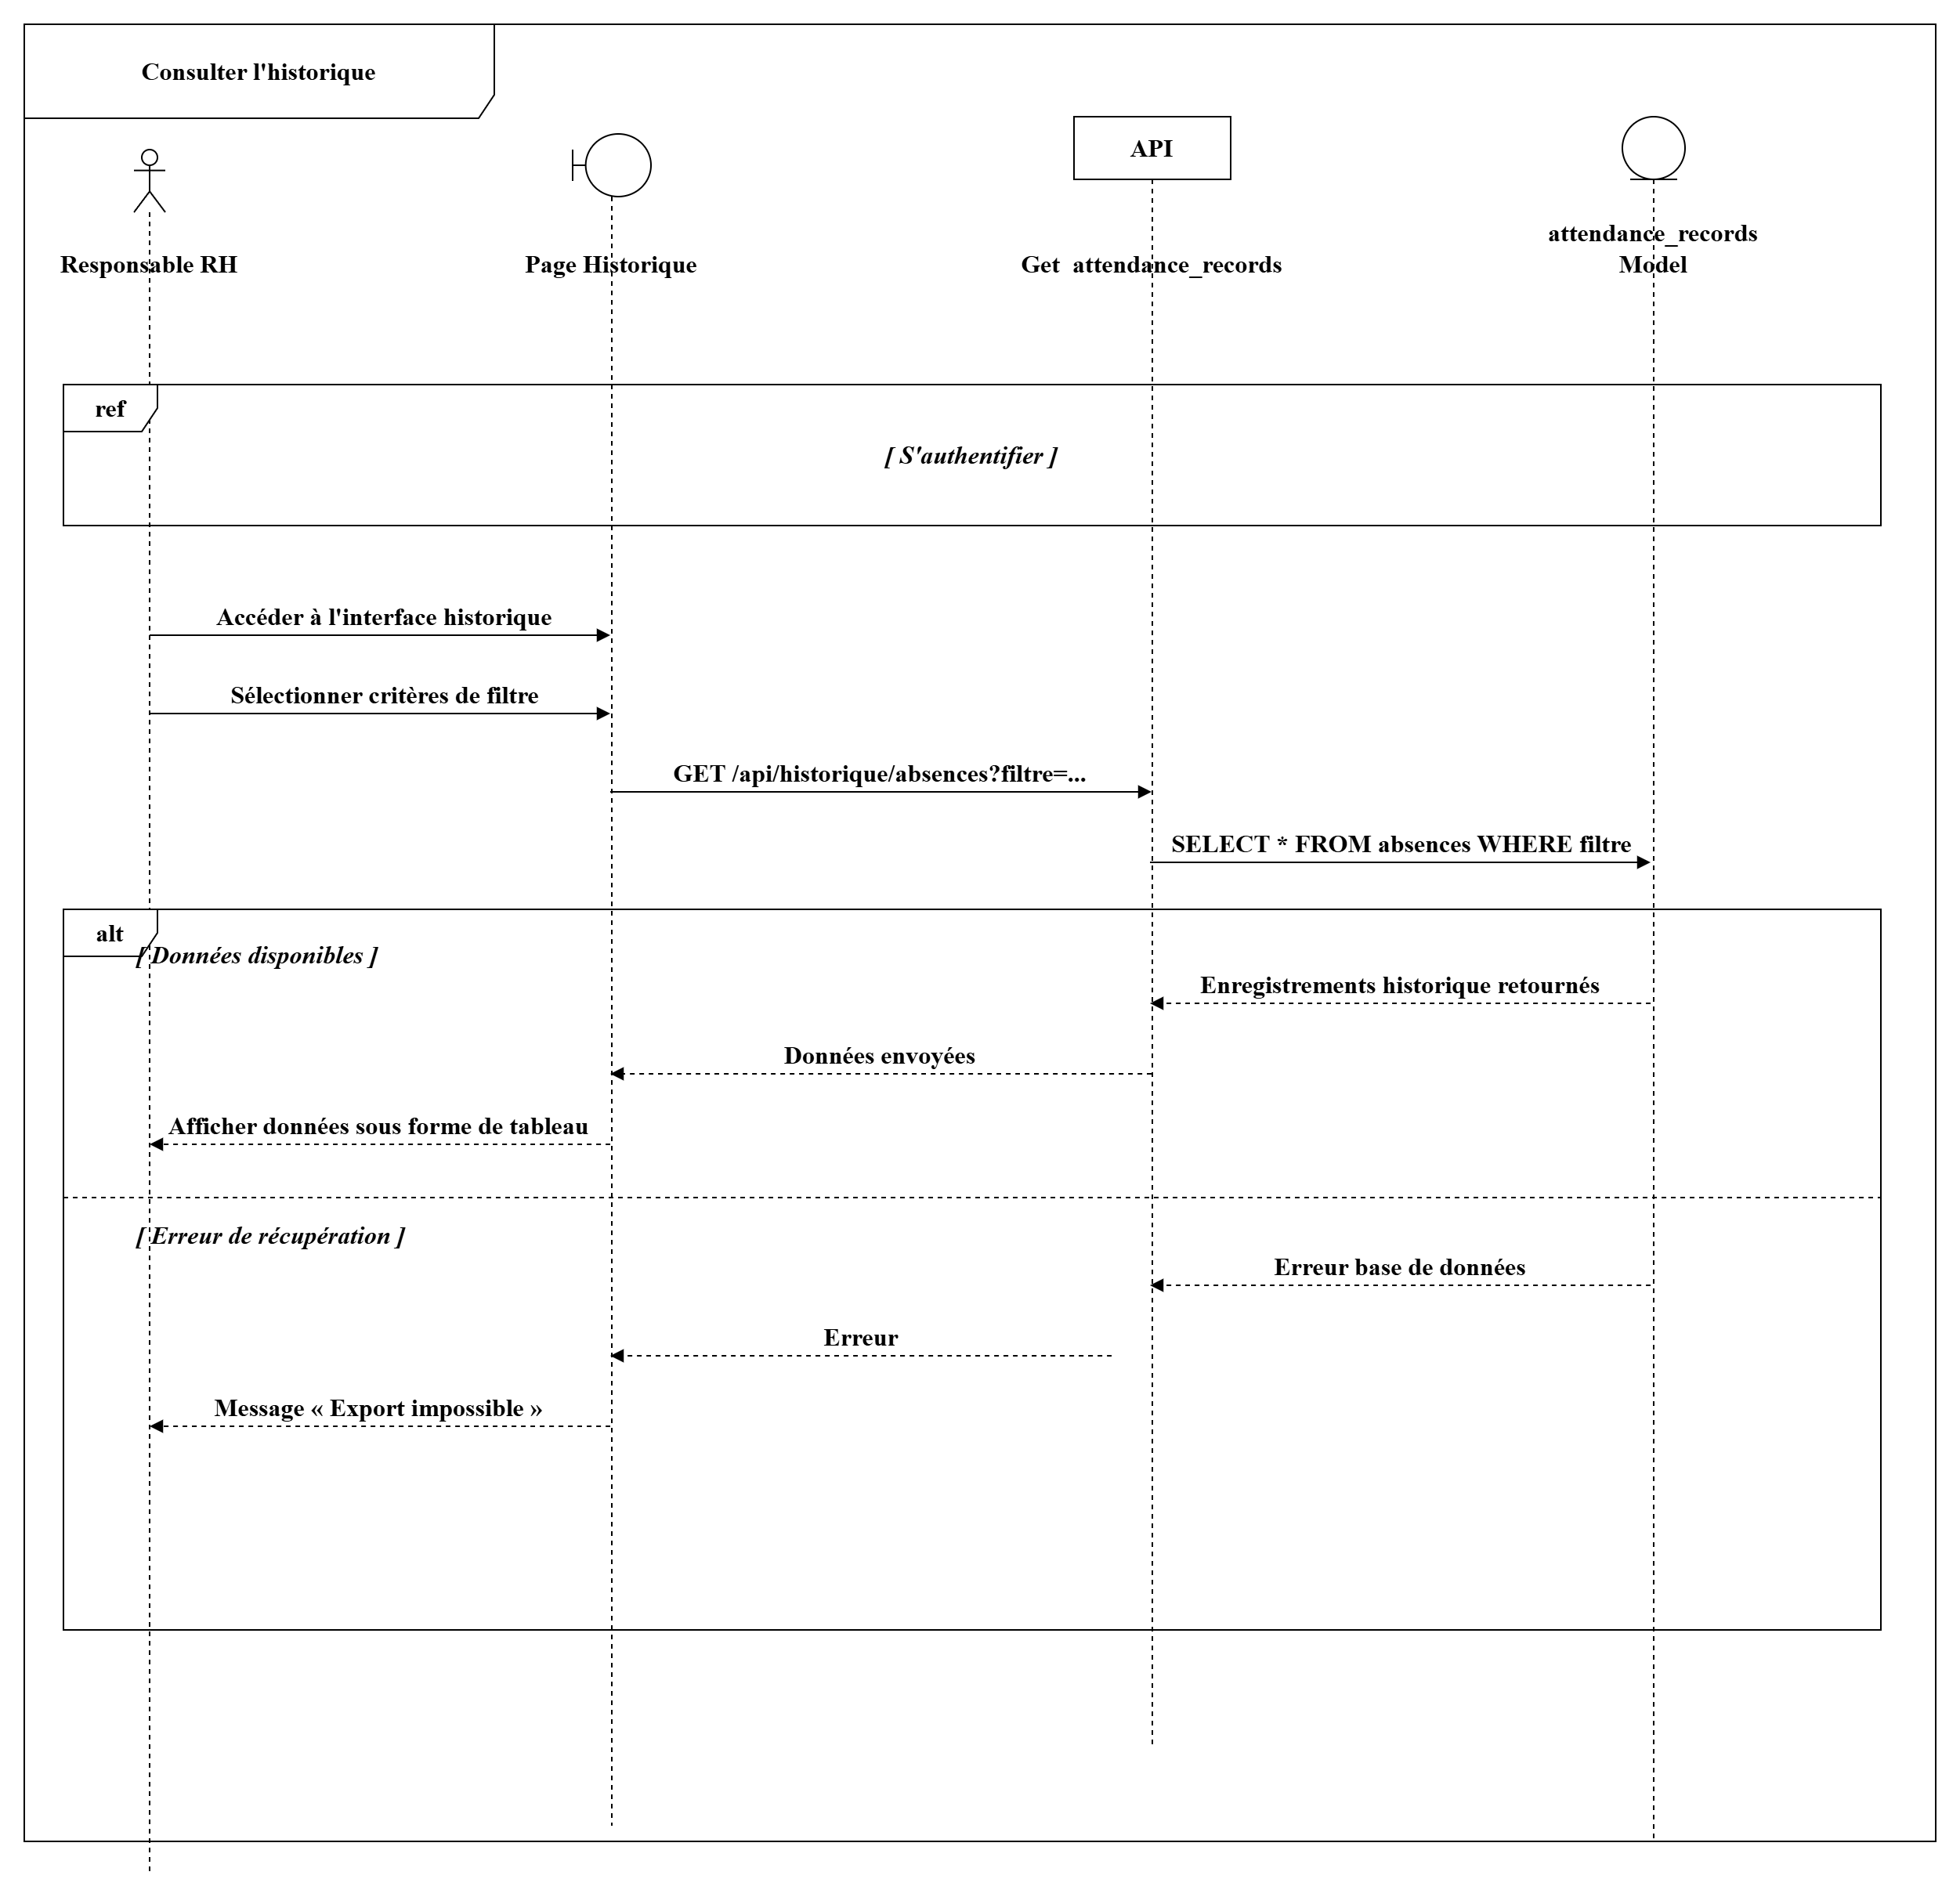
\includegraphics[width=0.9\textwidth]{projet/images/sequence s4/c historique.drawio.png}
    \caption{Diagramme de séquence du cas d'utilisation «~Consulter historique~»}
\end{figure}

\item[$\bullet$] \textbf{Diagramme de séquence du cas d'utilisation «~Exporter rapport~»}



\begin{figure}[H]
    \centering
    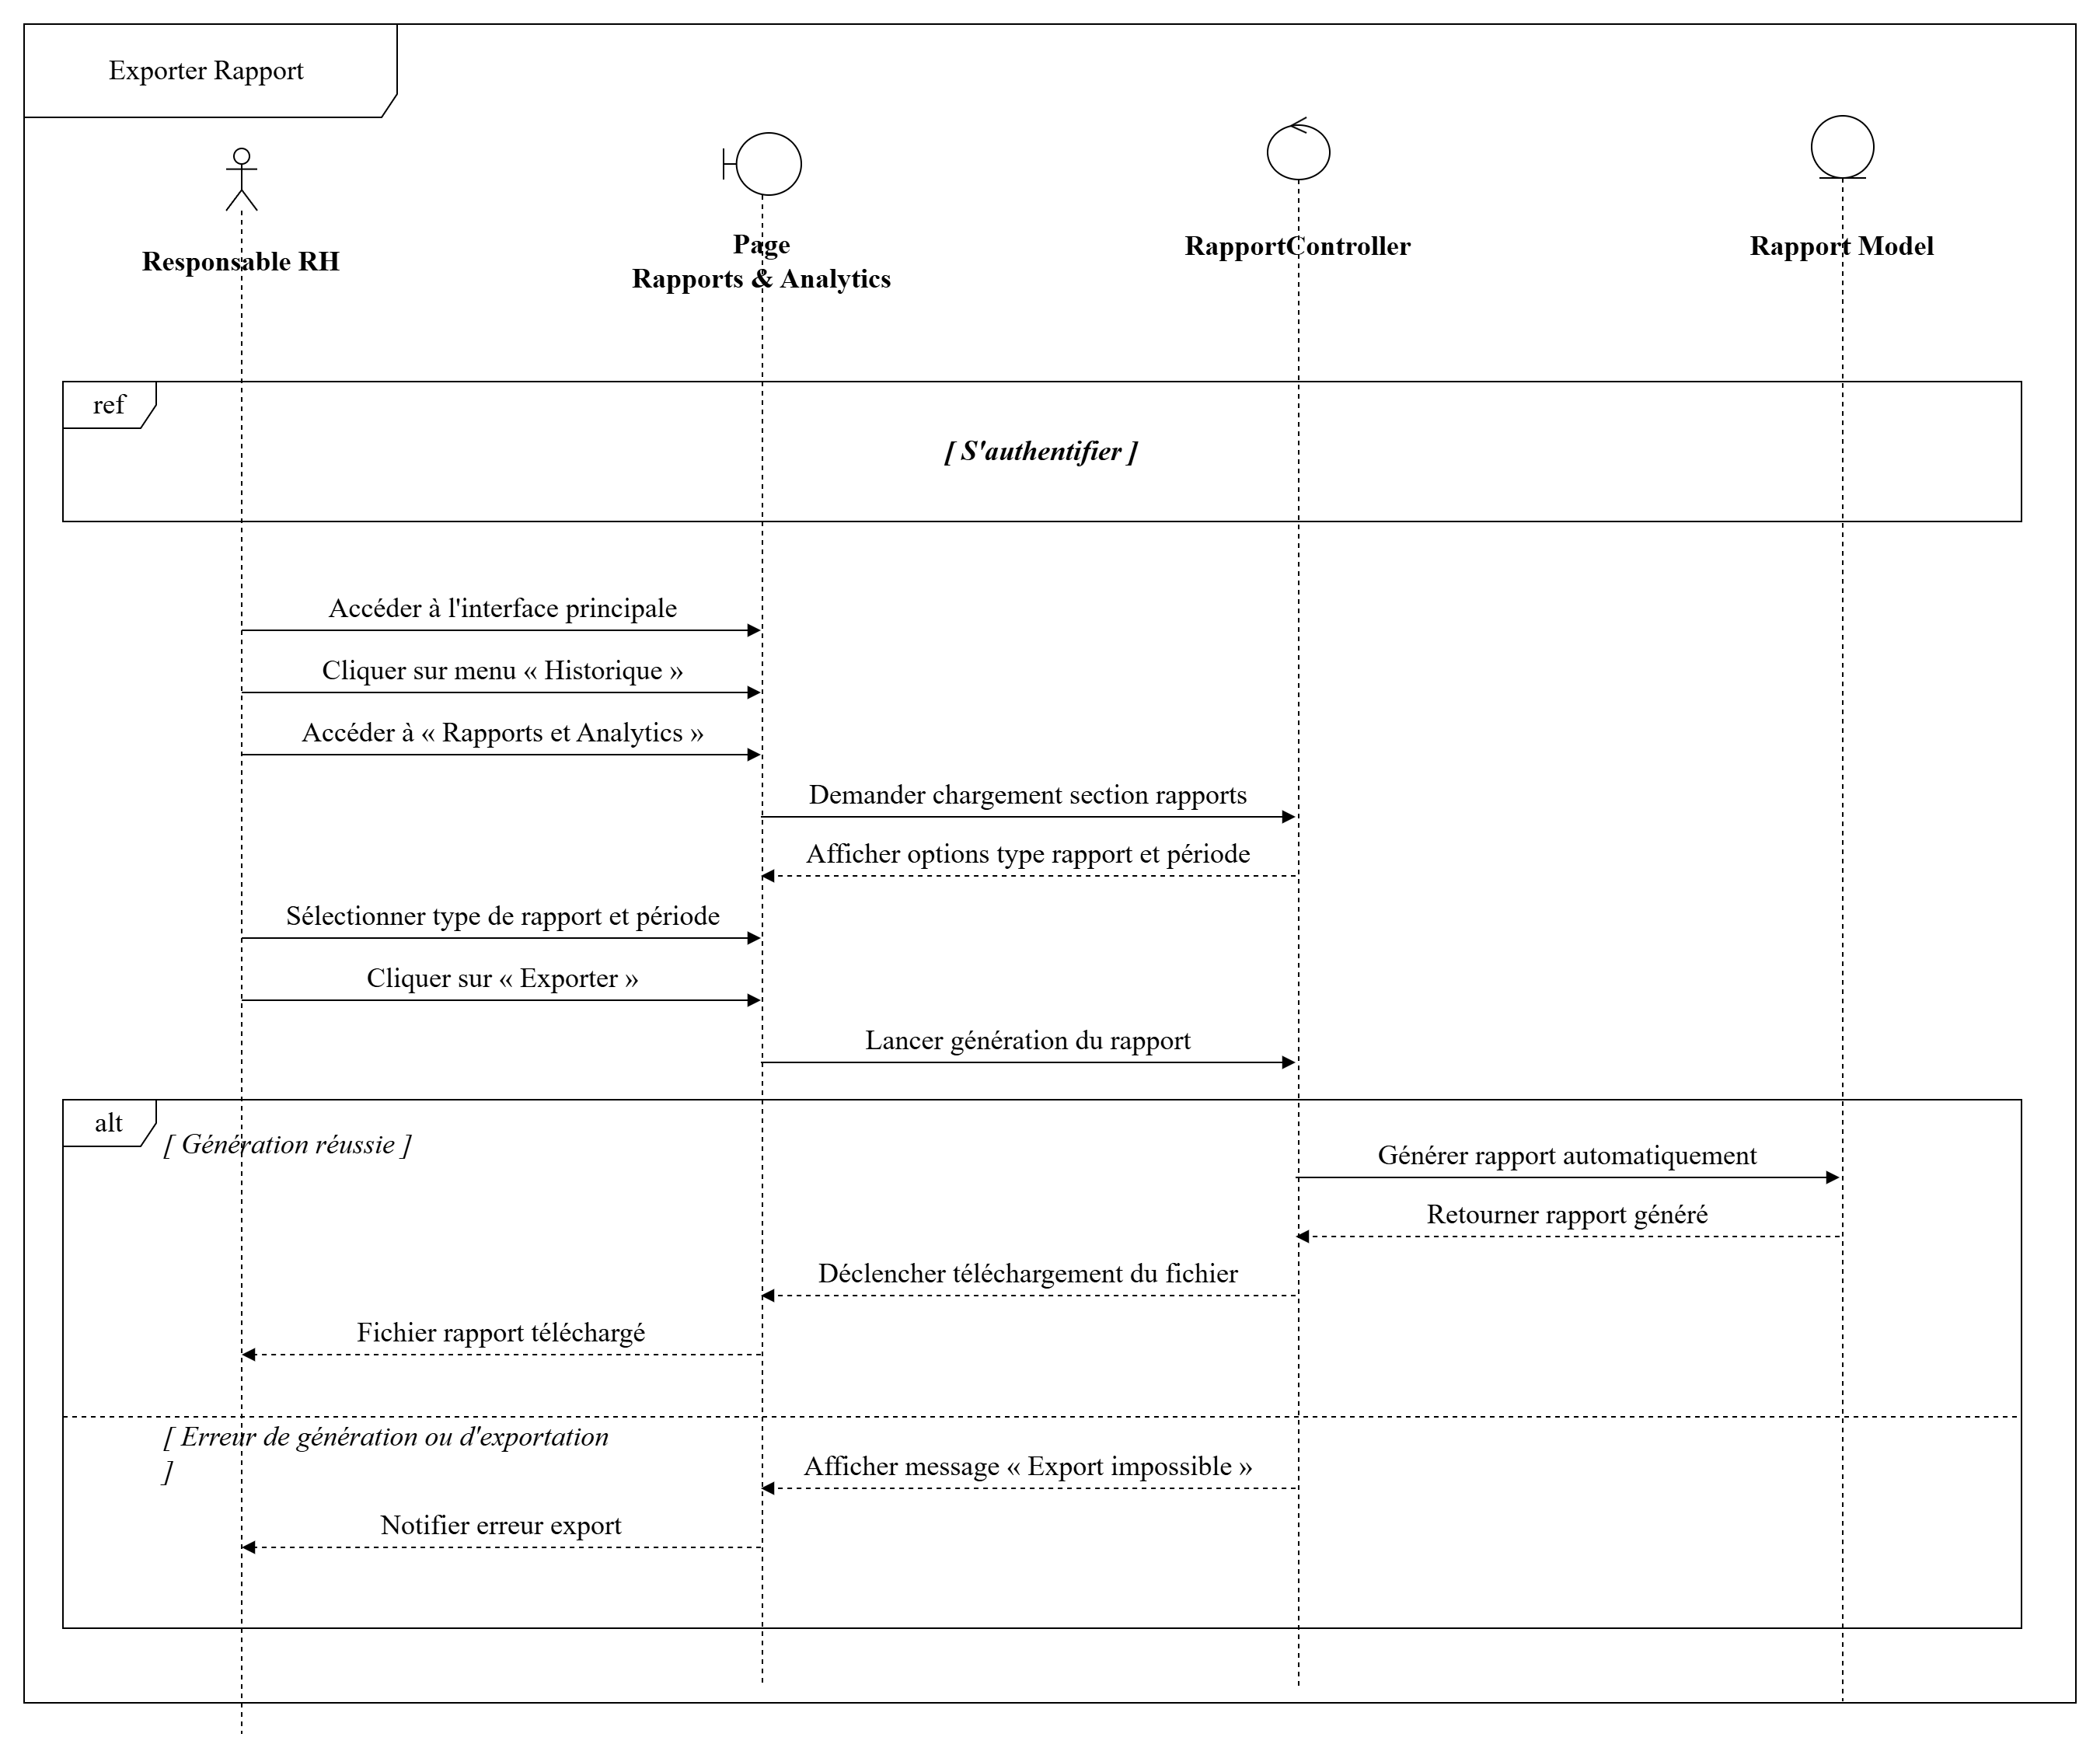
\includegraphics[width=0.9\textwidth]{projet/images/sequence s4/exporte.drawio.png}
    \caption{Diagramme de séquence du cas d'utilisation «~Exporter rapport~»}
\end{figure}

\end{itemize}

\subsection{Interfaces réalisées pour le sprint 4}

\begin{itemize}

\item[$\bullet$] \textbf{Dashboard Administrateur}

Cette page permet à l’administrateur de surveiller le fonctionnement global de la plateforme RH.  
Elle affiche les statistiques principales, les activités récentes et les informations importantes du système afin d’assurer une bonne gestion de la plateforme.

\begin{center}
    \begin{figure}[H]
        \centering
        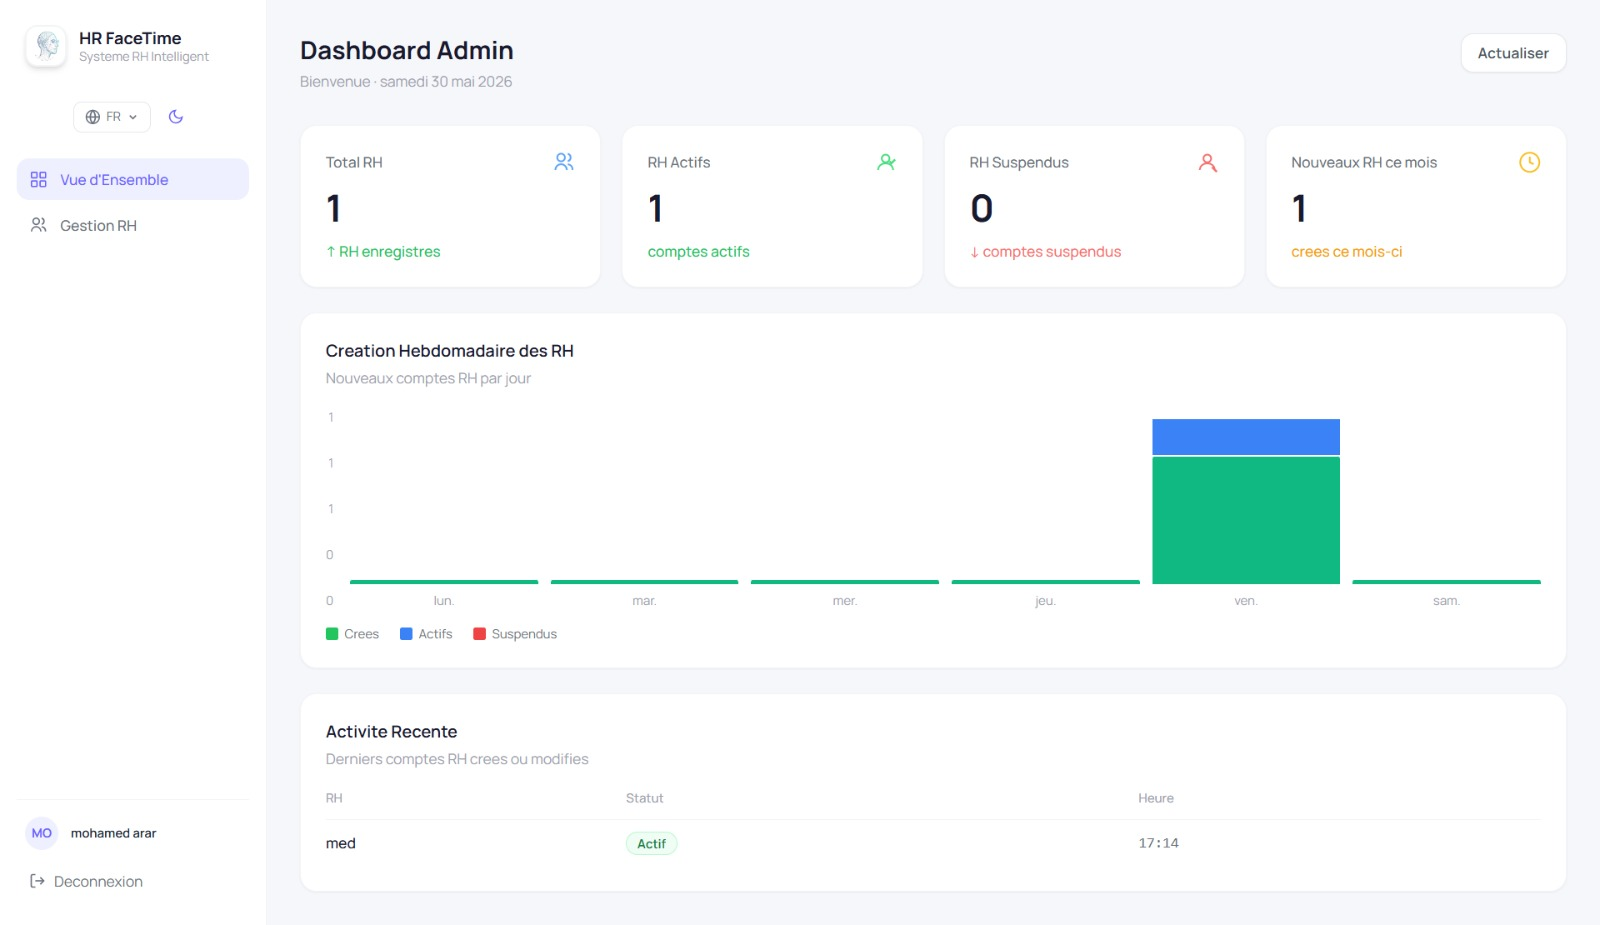
\includegraphics[width=0.9\textwidth]{projet/images/interface/s4/dashbord_admin.jpg}
        \caption{Interface du Dashboard Administrateur}
    \end{figure}
\end{center}

\item[$\bullet$] \textbf{Dashboard Responsable RH}

Cette page permet au responsable RH de visualiser les indicateurs liés aux employés, aux absences, aux congés et aux salaires.  
Elle facilite le suivi et le pilotage des activités RH de l’entreprise.

\begin{center}
    \begin{figure}[H]
        \centering
        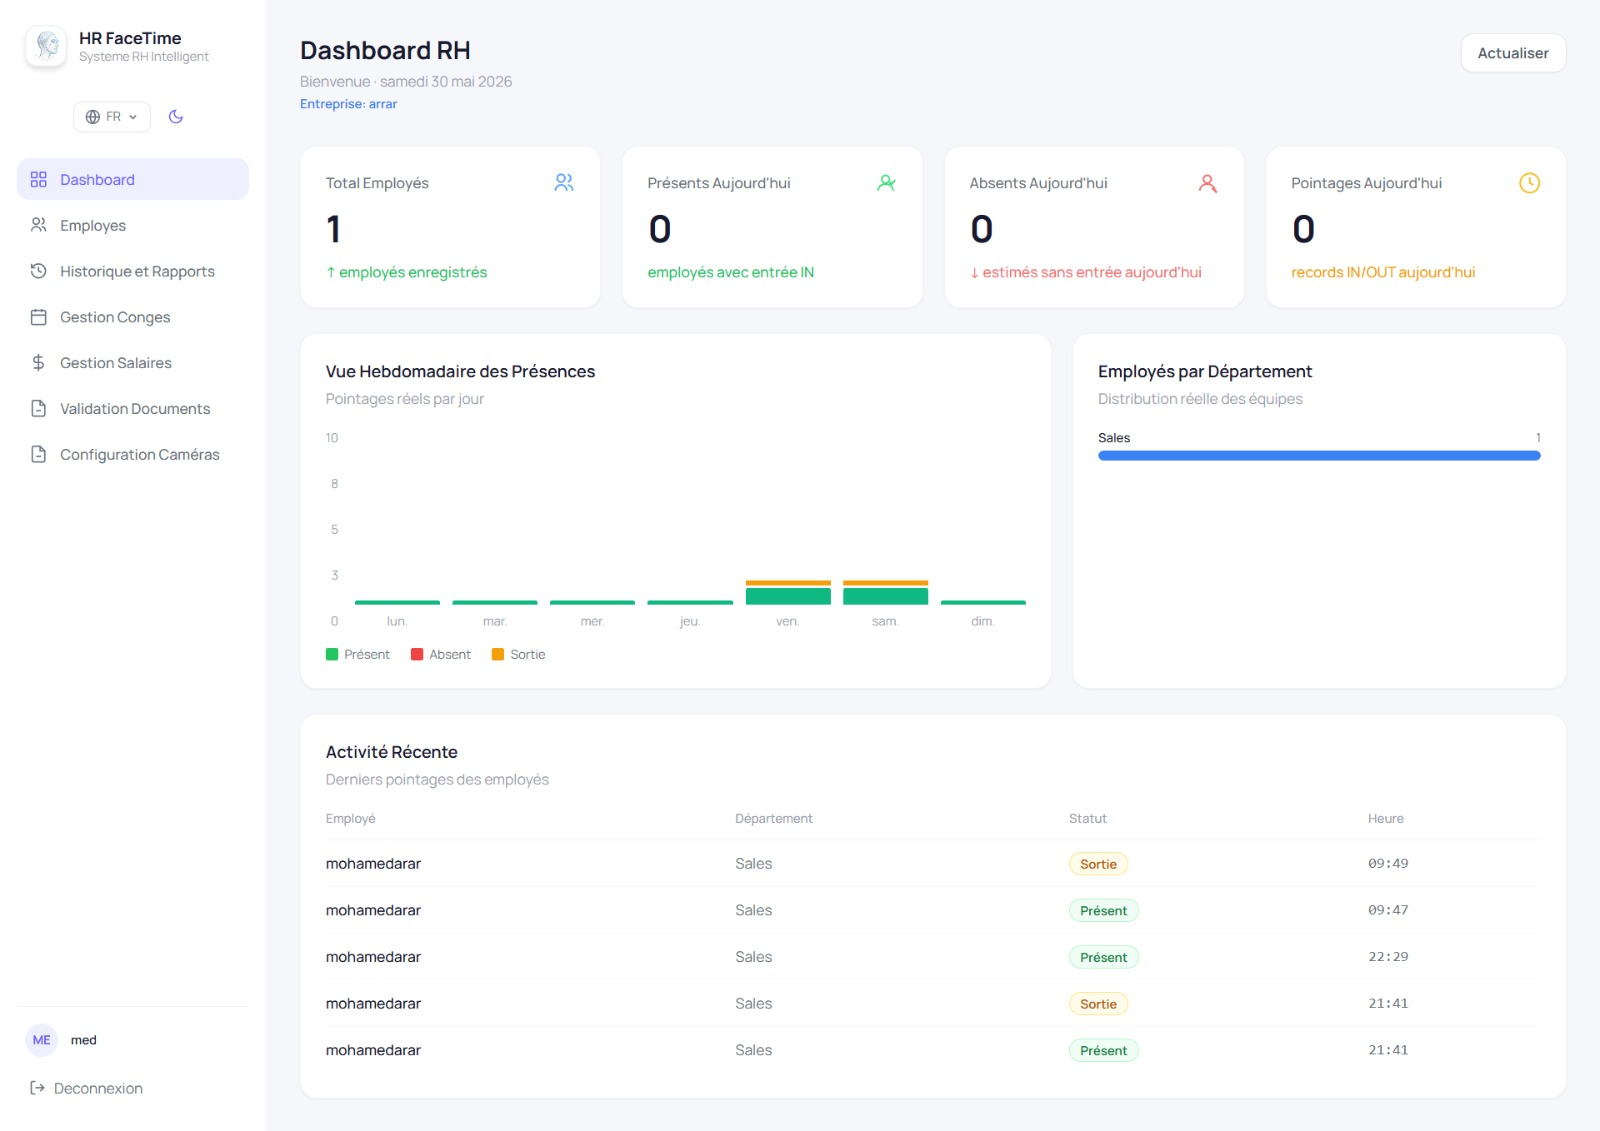
\includegraphics[width=0.9\textwidth]{projet/images/interface/s4/rh.jpeg}
        \caption{Interface du Dashboard Responsable RH}
    \end{figure}
\end{center}

\item[$\bullet$] \textbf{Exportation des Rapports}

Cette page permet de générer et télécharger différents rapports RH sous plusieurs formats.  
Elle aide à analyser les données administratives et à produire des documents de suivi.

\begin{center}
    \begin{figure}[H]
        \centering
        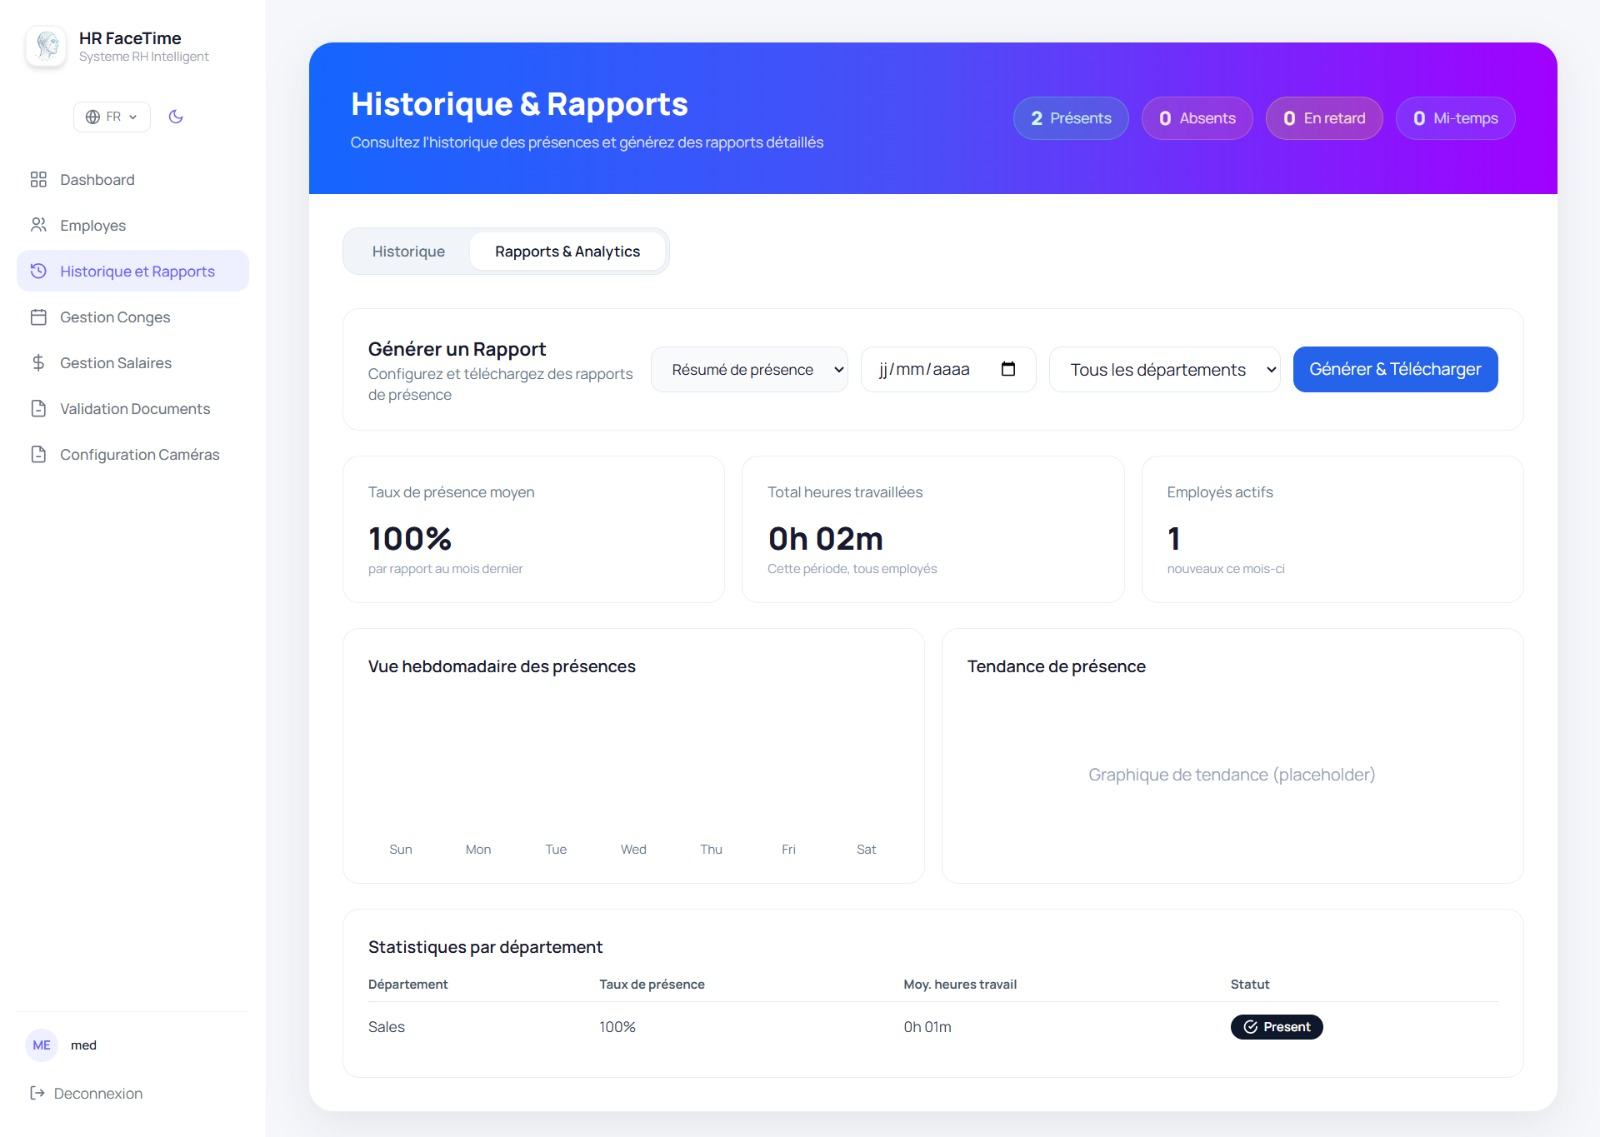
\includegraphics[width=0.9\textwidth]{projet/images/interface/s4/rapport.jpg}
        \caption{Interface d'exportation des rapports}
    \end{figure}
\end{center}


\item[$\bullet$] \textbf{ Consulter historique }

Cette page permet de consulter l’historique des actions effectuées sur la plateforme RH.  
Elle assure la traçabilité et le suivi des opérations réalisées par les utilisateurs.

\begin{center}
    \begin{figure}[H]
        \centering
        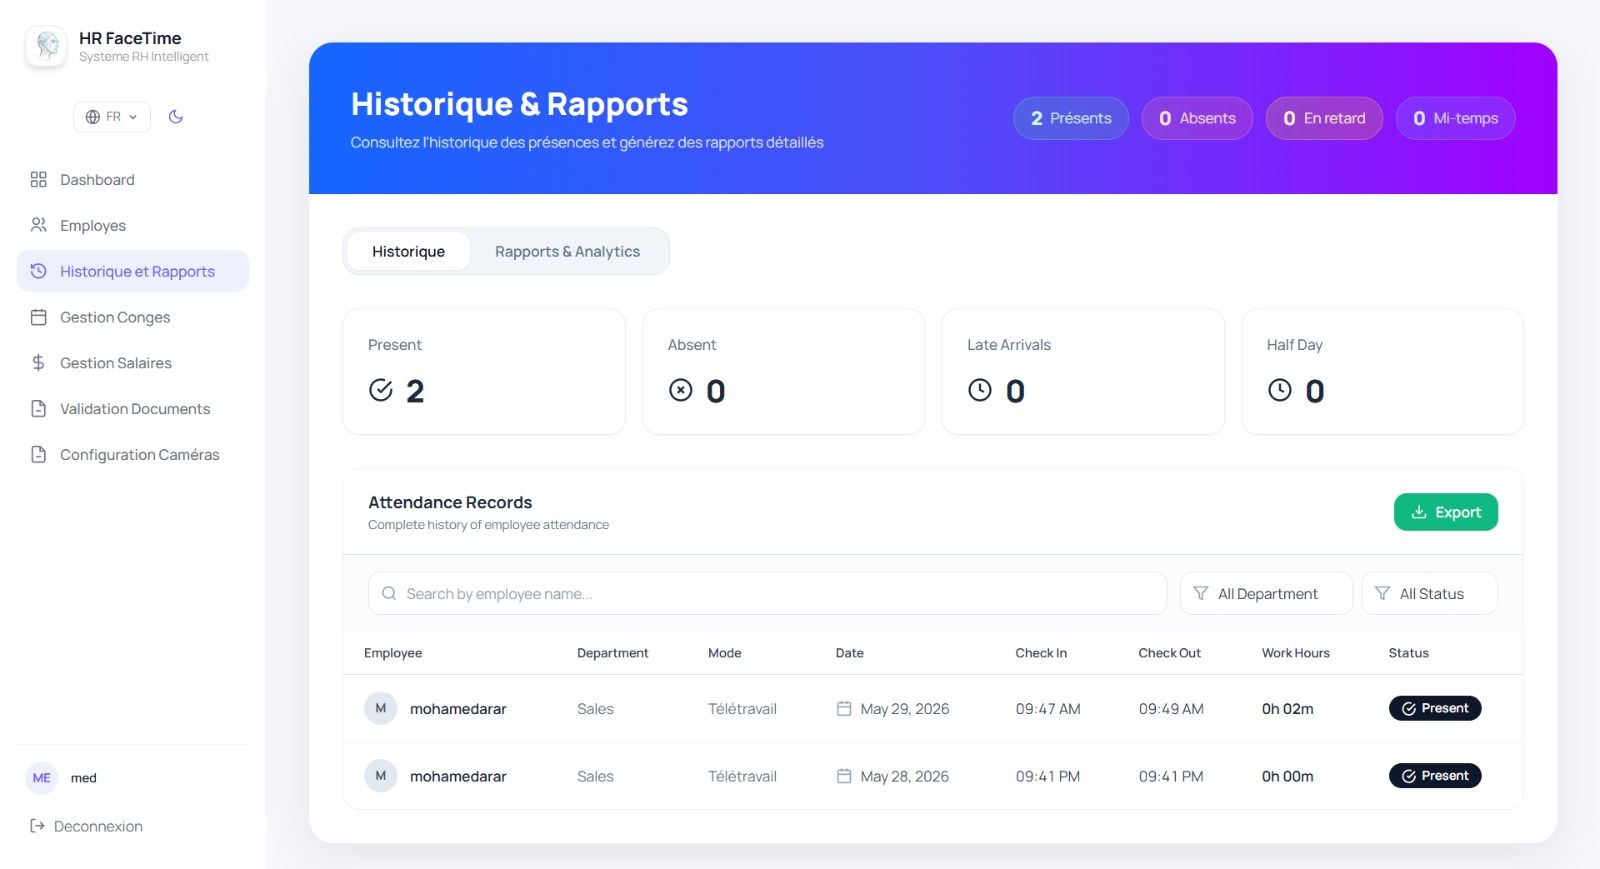
\includegraphics[width=0.9\textwidth]{projet/images/interface/s4/historique.jpg}
        \caption{Interface de Consulter historique}
    \end{figure}
\end{center}

\end{itemize}

\section{Conclusion}
Dans ce chapitre, nous avons présenté les livraisons des sprints 3 et 4, correspondant à la Release 2 du projet. Les fonctionnalités de gestion RH (congés, documents, primes, salaires) ainsi que les modules de statistiques, rapports et abonnement ont été détaillés à travers les backlog, spécifications fonctionnelles, conceptions et interfaces réalisées. Cette release constitue le produit final fonctionnel et complet du projet.

%==============================================================
% CONCLUSION
%==============================================================

\cleardoublepage
\chapter*{Conclusion générale et Perspectives}
%ajouter le titre introduction générale dans la table des matières
\addcontentsline{toc}{chapter}{Conclusion générale et Perspectives}
%définir l'entête de ce chapitre 
\markboth{Conclusion générale et Perspectives}{}
\setlength{\intextsep}{6pt}
\setlength{\textfloatsep}{8pt}
\setlength{\floatsep}{6pt}
\setlength{\abovecaptionskip}{3pt}
\setlength{\belowcaptionskip}{1pt}
\setlength{\LTpre}{3pt}
\setlength{\LTpost}{3pt}

En conclusion, le projet de conception et de développement d’un logiciel RH intelligent de pointage automatique basé sur la reconnaissance faciale met en évidence l’importance de l’intégration des technologies innovantes dans la gestion des ressources humaines. Cette solution permet d’automatiser le processus de pointage, de réduire les erreurs humaines et de renforcer la fiabilité des données liées à la présence des employés.  
Grâce à l’utilisation de technologies modernes telles que \textbf{Next.js}, \textbf{Flask} et \textbf{MySQL}, ainsi que l’intégration de l’intelligence artificielle, le système offre une gestion efficace, sécurisée et optimisée des informations. Il contribue également à améliorer la productivité des entreprises tout en simplifiant les tâches administratives.

En se tournant vers l’avenir, plusieurs perspectives d’amélioration et d’évolution peuvent être envisagées :
\begin{itemize}
    \item \textbf{Amélioration du modèle de reconnaissance faciale} : Augmenter la précision et la robustesse du système dans différentes conditions (éclairage, angles, etc.).
    \item \textbf{Renforcement de la sécurité} : Intégrer des mécanismes avancés tels que l’authentification multi-facteurs et la protection des données biométriques.
    \item \textbf{Développement d’une application mobile} : Permettre aux employés et aux administrateurs d’accéder au système via une application mobile pour faciliter le pointage et la gestion à distance.
    \item \textbf{Déploiement en cloud} : Assurer une meilleure disponibilité, scalabilité et accessibilité du système.
\end{itemize}

En exploitant ces perspectives, ce logiciel pourra évoluer vers une solution complète et intelligente de gestion des ressources humaines, capable de répondre aux besoins croissants des entreprises tout en s’inscrivant dans une démarche d’innovation technologique continue.

%==============================================================
% RÉFÉRENCES
%==============================================================

\cleardoublepage
\bibliographystyle{plain}

\begin{thebibliography}{99}

% FIX chapitre1
\bibitem{ref1}
unibro Inc., \textit{unibro }, \url{https://unibro.net/}, 2024.

\bibitem{scrum_guide}
« Scrum », 2026. Disponible sur : \url{https://www.atlassian.com/fr/agile/scrum} (consulté le 05/02/2026).

% FIX chapitre2 — Outils de conception
\bibitem{figma}
Figma Inc., \textit{Figma — Interface Design Tool}, \url{https://www.figma.com}, 2024.

\bibitem{photoshop}
Adobe Inc., \textit{Adobe Photoshop}, \url{https://www.adobe.com/products/photoshop.html}, 2024.

\bibitem{drawio}
JGraph Ltd., \textit{Draw.io — Diagramming Tool}, \url{https://www.draw.io}, 2024.

\bibitem{overleaf}
Overleaf Documentation, \textit{LaTeX Tutorials}, \url{https://docs.overleaf.com/getting-started/latex-tutorials}, 2024.

% FIX chapitre2 — Outils de développement
\bibitem{Visual Studio Code}
Microsoft, \textit{Visual Studio Code}, \url{https://code.visualstudio.com}, 2024.

\bibitem{GitHub}
GitHub Inc., \textit{GitHub — Code Hosting Platform}, \url{https://github.com}, 2024.

\bibitem{Postman}
Postman Inc., \textit{Postman — API Platform}, \url{https://www.postman.com}, 2024.

% FIX chapitre2 — Langages
\bibitem{HTML}
W3C, \textit{HTML5 Specification}, \url{https://www.w3.org/TR/html52/}, 2017.

\bibitem{CSS}
W3C, \textit{CSS Snapshot}, \url{https://www.w3.org/TR/CSS/}, 2023.

\bibitem{JavaScript}
ECMA International, \textit{ECMAScript 2023 Language Specification}, \url{https://www.ecma-international.org}, 2023.

\bibitem{TypeScript}
Microsoft, \textit{TypeScript Documentation}, \url{https://www.typescriptlang.org}, 2024.

\bibitem{Python}
Python Software Foundation, \textit{Python 3 Documentation}, \url{https://docs.python.org/3/}, 2024.

\bibitem{SQL}
ISO/IEC, \textit{SQL:2016 Standard}, ISO, 2016.

% FIX chapitre2 — Frameworks et bibliothèques
\bibitem{Next.js}
Vercel, \textit{Next.js Documentation}, \url{https://nextjs.org/docs}, 2024.

\bibitem{React}
Meta Open Source, \textit{React Documentation}, \url{https://react.dev}, 2024.

\bibitem{Flask}
Pallets Projects, \textit{Flask Documentation}, \url{https://flask.palletsprojects.com}, 2024.

\bibitem{OpenCV}
OpenCV Team, \textit{OpenCV Documentation}, \url{https://docs.opencv.org}, 2024.

\bibitem{MediaPipe}
Google LLC, \textit{MediaPipe Solutions}, \url{https://developers.google.com/mediapipe}, 2024.

\bibitem{TensorFlow}
Google Brain Team, \textit{TensorFlow Documentation}, \url{https://www.tensorflow.org}, 2024.

\end{thebibliography}

\end{document}
